\documentclass[oneside]{ctexbook}
% \usepackage{lmodern}
\usepackage[margin=2cm]{geometry}
\usepackage[dvipsnames]{xcolor}
\usepackage{caption}

% Create Example enviornment
\usepackage{fontspec}
\usepackage[most]{tcolorbox}
\tcbuselibrary{skins,breakable}
\usepackage{xparse}
\usepackage[colorlinks,linkcolor=blue]{hyperref}
\usepackage{xurl}
\usepackage{cleveref}

% 设置example环境
\newtcolorbox[auto counter, number within=chapter, 
    crefname={example}{examples},
    Crefname={Example}{Examples},
    number freestyle={\noexpand\thechapter.\noexpand\arabic{\tcbcounter}}]
    {example}[2][]{%
    enhanced,
    breakable,
    fonttitle=\bfseries,
    colback=NavyBlue!5!white,
    % opacityback=0,
    % opacityfill=0,
    colbacktitle=OliveGreen!80!white,
    title=示例~\thetcbcounter: #2,    
    #1
}

% 设置代码环境
\newtcolorbox[auto counter, number within=chapter, 
    crefname={code}{codes},
    Crefname={Code}{Codes},
    number freestyle={\noexpand\thechapter.\noexpand\arabic{\tcbcounter}}]
    {code}[2][]{%
    enhanced,
    breakable,
    fonttitle=\bfseries,
    boxrule=0pt,
    frame hidden,
    colback=black!100!white,
    opacityback=0,
    colbacktitle=NavyBlue!80!white,
    title=\textbf{代码~\thetcbcounter} #2,    
    #1
}

% 设置Note环境
\newtcolorbox[auto counter, number within=chapter, 
    crefname={note}{notes},
    Crefname={Note}{Notes},
    number freestyle={\noexpand\thechapter.\noexpand\arabic{\tcbcounter}}]
    {note}[2][]{%
    enhanced,
    breakable,
    fonttitle=\bfseries,
    boxrule=1pt,
    % frame hidden,
    colback=BrickRed!5!white,
    colbacktitle=BrickRed!80!white,
    title=\textbf{#2},    
    #1
}

% Minted Code Highlight
\usepackage{listings}
\usepackage[newfloat]{minted}
\setminted{
    autogobble=true,
    obeytabs=true,
    tabsize=4,
    breaklines, % 自动断行
    frame=leftline, % 加边框
    framesep=2pt, % 边框与代码的间距
    fontsize=\small, % 字体大小
    linenos, % 显示行号
    % bgcolor=black
}
\usemintedstyle{tango}

% \DeclareCaptionFormat{listing}{%
% \colorbox{NavyBlue}{\textcolor{white}{\parbox{\dimexpr\textwidth-2\fboxsep-2\fboxrule\relax}{\textbf{#1}#2 #3}}}
% } 
% % \DeclareCaptionFormat{listing}{\colorbox{NavyBlue}{\textcolor{white}{\textbf{#1 #2 #3}}}}
% \newenvironment{code}{\captionsetup{type=listing}}{}
% \SetupFloatingEnvironment{listing}{name=\textbf{代码}}
% \captionsetup[listing]{format=listing,singlelinecheck=false, margin=0pt, font={sc,color=white}}

\usepackage{longtable}
\usepackage{booktabs}
\usepackage{array} 

\usepackage{graphicx}
\graphicspath{{images/}}

\usepackage{pagenote}
%% 在每章末尾将注释列为一节
\renewcommand*{\notedivision}{\section*{\notesname}}
\renewcommand*{\pagenotesubhead}[1]{}
%%%%%%%%%%%%% 章末注样式设置(可选)不需要的话注释掉
% 每一个注释编号前添加章节号,形如:3-14
% \renewcommand{\thepagenote}{\thechapter-\arabic{pagenote}}
% 正文中注释编号样式调整:上标,小号字,方括号
\renewcommand\notenumintext[1]{\textsuperscript{\footnotesize[#1]}}
% 章节末尾注释编号样式调整:方括号,正常大小
\renewcommand\notenuminnotes[1]{{[#1] }}
% 更换注释一节标题为中文
\renewcommand{\notesname}{注释}
%%%%%%%%%%%%% End customisation
%% !必须要有下面这行!
\makepagenote


\begin{document}

\title{Elixir与OTP精简指南}
\author{原作者:Benjamin Tan Wei Hao \\翻译:林懿伦}
\date{}
\maketitle

\phantomsection
\tableofcontents
\addcontentsline{toc}{chapter}{目录}

\chapter*{欢迎}\label{welcome}
\addcontentsline{toc}{chapter}{欢迎}

感谢您购买《Elixir和OTP精简指南》! 在您阅读这本书的时候,我可能还在为这本书终于出版而和我的妻子击掌庆祝。

为了充分享受这本中级水平的书籍,我假设您是一个聪明的人,并且已经有一些编程经验(最好是Web开发方面的)了。幸运的是,您不必了解Elixir或Erlang,尽管手边有相关文档会有所帮助。

Elixir是一种新的函数式编程语言,建立在传奇的Erlang VM之上。OTP是一个经过实战测试的框架(Erlang伟大之源),使您能够构建具有容错性和可扩展性的应用程序。

这对您意味着什么?这意味着我将向您展示一些您可以使用Elixir和OTP框架构建的令人敬畏的东西。我努力使这本书尽可能地接近读者,并且更重要的是,尽可能地有趣。
通过一系列例子,您将学会编写并发程序,看看将您的应用程序组合起来使其具有容错性是多么容易,以及构建具有实时连接能力的Web应用程序。

在阅读时,我希望您能够利用在线作者论坛。我将阅读您的评论并做出回应,您的反馈对于开发过程非常有帮助。

再次感谢您对我的首次出版的支持。我相信您会喜欢这本书的!

\vspace{2cm} 

\hspace{0.5\textwidth}\textit{Benjamin Tan Wei Hao}


\chapter*{前言}\label{preface}
\addcontentsline{toc}{chapter}{前言}

当我想出这本书的标题时,我认为这是相当聪明的。用``精简''和``指南''这样的词暗示读者可以期待一本相对较薄的书。这意味着我不需要编写太多的内容。这很好,因为Elixir是一种非常新的语言,几乎没有什么社区可以谈论。那是在2014年,Elixir还是0.13版本,Phoenix还只是一个网络套接字库。

两年过去了,三百页的书也随之完成。语言经历了许多变化,社区也在成长。对Elixir的兴奋无疑是明显的,从众多博客文章和推文中可以看出。公司也开始发现并爱上了Elixir。甚至对Erlang也有了重新的兴趣,如果你问我,这绝对是一个奇妙的现象!

这本书是我尝试传播这门语言的谦卑尝试。我最喜欢通过例子来学习,我假设你也是一样。我尽力使例子有趣、贴近生活,但最重要的是,启发性和实用性。

花了两年多的时间写这本书,我非常兴奋终于可以把这本书交到你手上。我希望这本书能给你带来我在使用Elixir编程时所体验到的同样的快乐。你还在等什么呢?

\chapter*{关于本书}\label{about}
\addcontentsline{toc}{chapter}{关于本书}

嗨,欢迎光临!Elixir 是一种构建在 Erlang
虚拟机上的函数式编程语言。它结合了 Ruby 的生产力和表现力以及 Erlang
的并发性和容错性。Elixir 充分利用了 Erlang 强大的 OTP
库,许多开发者认为这是 Erlang
伟大的源泉,因此你可以立即拥有成熟、专业品质的功能。Elixir
对函数式编程的支持使其成为高度分布式的事件驱动应用程序(如物联网系统)的绝佳选择。

本书尊重您的时间,旨在尽最小的麻烦带您快速了解 Elixir 和
OTP。然而,它期望您投入必要的工作量来掌握所有各种概念。因此,当您尝试实例并进行实验时,本书效果最佳。如果您遇到困难,请不要烦恼
- Elixir 社区非常欢迎新手!

\section*{书籍组织方式}

本书分为三部分,共十一章,还有一个附录。第一部分涵盖了 Elixir 和 OTP
的基础知识。

第一章介绍 Elixir,它与其父语言 Erlang
的不同之处,与其他语言的比较,以及 Elixir 和 OTP 的用例。

第二章带您快速了解 Elixir。您将编写您的第一个 Elixir
程序,并熟悉语言基础。

第三章介绍进程,Elixir 的并发单位。您将了解 Actor
并发模型,以及如何使用进程发送和接收消息。然后,您将组装一个示例程序,以查看并发进程的实际操作。

第四章介绍 OTP,这是 Elixir 从 Erlang 继承的杀手级特性之一。您将了解 OTP
的哲学,以及作为 Elixir 程序员将使用的 OTP 中最重要的部分。您将了解 OTP
行为的工作方式,并使用 GenServer 行为构建您的第一个 Elixir/OTP 应用程序
- 一个与第三方服务通信的天气程序。

第二部分涵盖了 Elixir 和 OTP
的容错和分布式方面。第五章查看处理错误的基本原理,特别是在并发环境中。您将了解
Erlang VM
在处理进程崩溃时所采取的独特方法。您还将体验构建自己的监督进程(类似于
Supervisor OTP 行为),然后使用真实的 Supervisor。

第六章全面讨论 Supervisor OTP 行为和容错。您将了解 Erlang
的``让它崩溃''哲学。本章介绍了使用前几章建立的技能的工作池应用程序。

第七章继续讨论工作池,我们在其中添加更多功能,使其成为更全面和现实的工作池应用程序。在此过程中,您将学习如何构建非平凡的监督层次结构,并学习如何动态创建监督和工作进程。

第八章考察分布式及其在负载平衡方面的帮助。它指导您构建一个分布式负载平衡器。同时,您将学习如何在
Elixir 中构建命令行程序。

第九章继续讨论分布式,但这次我们着眼于故障转移和接管。这对于必须对故障具有弹性的任何非琐碎应用程序来说都是绝对关键的。您将构建一个既具有容错性又具有分布式特性的
Chuck Norris 笑话服务。

第三部分涵盖了 Elixir
中的类型规范、基于属性的测试和并发测试。我们将研究三种工具,即
Dialyzer、QuickCheck 和
Concuerror,并查看这些工具如何帮助我们编写更好、更可靠的 Elixir 代码。

附录提供了在您的机器上设置 Erlang 和 Elixir 的说明。

\section*{谁应该阅读这本书}

您手头没有太多时间。您想看看 Elixir 的热闹是什么,尽快动手实践。

我假设您熟悉终端操作并具有一些编程经验。

虽然事先了解 Elixir 和 Erlang
当然有帮助,但绝不是必须的。然而,本书并不打算作为 Elixir
的参考书。您应该知道如何自行查找文档。

您也不排斥变化。Elixir
变化很快。但是,您正在阅读这本书,所以我假设这对您来说不是问题。

\section*{如何阅读这本书}

从前到后。本书的进展是线性的,虽然早期章节或多或少是独立的;但后面的章节是基于前面的章节构建的。一些章节可能需要重读,所以不要认为您应该在第一次阅读时就理解所有概念。

我最喜欢的编程书是那些鼓励您尝试代码的书。概念总是以这种方式更好地沉淀。在这本书中,我也力求达到同样的效果。没有什么比动手实践更有益了。一些章节的结尾有练习。\textbf{做它们!}在头脑清晰、终端打开、渴望学习有趣且有价值的东西的情况下,这本书最有用。

\section*{获取示例代码}

最新的书籍代码托管在GitHub仓库: \url{https://github.com/benjamintanweihao/the-little-elixir-otp-guidebook-code}。

\section*{关于作者}

Benjamin Tan Wei Hao 是新加坡 Pivotal Labs的软件工程师。由于害怕变得无关紧要,他总是试图赶上他不断增长的阅读清单。他喜欢参加Ruby 会议并谈论 Elixir。

他还是 LeanPub 上一本自行出版的书《Ruby 闭包书》的作者。他还为 SitePoint的 Ruby 栏目撰稿,并试图偶尔插入一篇 Elixir文章。在他充裕的空闲时间里,他在 benjamintan.io 上写博客。


% Part 1
% \chapter*{第一部分 开始使用Elixir和OTP}\label{part1}
% \addcontentsline{toc}{chapter}{第一部分 开始使用Elixir和OTP}
\part{开始使用Elixir和OTP}\label{part1}

我们从Elixir的基础开始。我们将回答一些存在的问题,比如我们为什么需要Elixir,它有什么用。然后,我们将直接深入一系列示例,演示各种语言特性。

接下来,我们将探讨进程(processes),Elixir中并发的基本单元。我们将了解Elixir中的进程是如何与Actor并发模型相关的。如果你在其他语言中处理并发时遇到过困难,Elixir将是一股清新的空气。

我们将以介绍OTP结束第一部分,并学习GenServer行为,所有行为中最基本也是最重要的一个。

\chapter{概述}\label{chapt:intro}

本章涵盖内容包括:

\begin{itemize}
\item Elixir 是什么
\item Elixir 与 Erlang 的不同之处
\item 为什么选择 Elixir 而不是其他语言
\item Elixir/OTP 的适用场景
\item 未来的发展方向
\end{itemize}

如果你是因为药用目的购买了这本书 --- 很抱歉,这是本关于编程语言 Elixir的书。没有其他语言(除了Ruby)让我如此兴奋和乐于使用。即使在花了两年多时间写关于 Elixir的内容之后,我仍然热爱用它编程。

参与一个如此年轻而有活力的社区是一件非常特别的事情。我认为没有哪种语言在v1.0版本之前就已经有至少四本关于它的书、一系列的视频教程和一个会议了。我认为我们正在做一些真正有意义的事情。在深入了解Elixir 之前,我想先谈谈 Erlang 和它传奇的虚拟机,因为 Elixir是建立在它之上的。

Erlang是一种擅长构建软实时、分布式和并发系统的编程语言。它最初的用途是为爱立信的电话交换机编程。电话交换机基本上是连接来电者之间通话的机器。

这些交换机必须是并发的、可靠的和可扩展的。它们必须能够同时处理多个电话。它们还必须极其可靠。没有人希望自己的通话中途被切断。此外,由于软件/硬件故障导致的通话中断不应影响交换机上的其他通话。这些交换机必须能够大规模扩展,并与分布式网络中的其他交换机协同工作。

这些生产需求塑造了今天的Erlang。这些需求正是我们在多核和大规模网络环境中所面临的情况。

正如你将在后面的章节中发现的,Erlang虚拟机的调度器会自动在处理器之间分配工作负载。这意味着,如果你在一个拥有更多处理器的机器上运行程序,你几乎可以\emph{免费}获得速度提升。几乎,因为你需要改变你在Erlang 和 Elixir 中编写程序的思维方式,以获得全部好处。

编写分布式程序,即在不同计算机上运行且能够相互通信的程序,几乎不需要什么仪式性的工作。

现在是时候介绍 Elixir 了。Elixir 自称是\textbf{一个在 Erlang虚拟机之上构建的函数式(Functional)、元编程感知(meta-programming aware)的语言}。让我们逐一解析这个定义。

Elixir是一种\textbf{函数式}编程语言。这意味着它具有你可能期望的所有常见特性,如不可变状态、高阶函数、惰性求值和模式匹配。我们将在后面的章节中遇到所有这些特性以及更多。

Elixir也是一种具有元编程能力的语言。元编程可以描述为生成代码的代码(或者说,黑魔法)。这是可能的,因为代码可以用数据表示,数据也可以用代码表示。这些功能使程序员能够向语言添加新的结构(以及其他事物),而其他语言发现这些功能难以实现,甚至根本不可能实现。

这本书还涉及OTP,一个用于构建容错、可扩展和分布式应用程序的框架。与大多数框架不同,OTP附带了很多优秀的东西。OTP自带三种数据库、一套调试工具、性能分析工具、一个测试框架等等。虽然我们只能玩到一小部分,但这本书将让你体验到OTP 的纯粹精彩。

重要的是要意识到,Elixir本质上是免费获得OTP的,因为 OTP 是 Erlang分发的一部分。如果你想知道OTP是什么意思,简短的答案是它曾经被称为\textbf{开放电信平台(Open Telecom Platform)},这暗示了 Erlang的电信传统。这再次展示了计算机科学中命名是一个难题。这是因为OTP是一个通用框架,与电信几乎没有关系。如今,OTP 就是纯粹的 OTP,就像IBM现在只是 IBM 一样。

\section{Elixir和Erlang有什么不同}

在讨论Elixir与Erlang的不同之处之前,我们先来谈谈他们的\textbf{相似点}。Elixir和Erlang都会编译成相同的字节码。这意味着,无论是Elixir还是Erlang编写的程序,在编译后,都会生成在同一虚拟机上运行的指令。

Elixir的另一个优点是,你可以直接从Elixir调用Erlang代码,反之亦然!例如,如果你发现Elixir缺少Erlang中存在的某些功能,你可以直接从Elixir代码中调用Erlang库函数。

Elixir遵循了Erlang的大多数语义,如消息传递。大多数Erlang程序员会觉得使用Elixir非常自然。

这种互操作性也意味着,丰富的Erlang第三方库资源可以供Elixir开发者(也就是你)使用。那么,为什么你要选择使用Elixir而不是Erlang呢?至少有两个原因 - 工具和生态系统。

\section{工具}

开箱即用的,Elixir自带了一些实用工具:

\subsection{交互式Elixir}

交互式Elixir shell,简称为 \texttt{iex},是一个REPL(读取Read-求值Eval-打印Print 循环Loop),类似于Ruby的\texttt{irb}。它有一些非常棒的功能,如语法高亮和漂亮的文档系统,如图1.1所示。

\begin{figure}[htbp]
  \centering
  % 插入图片文件
  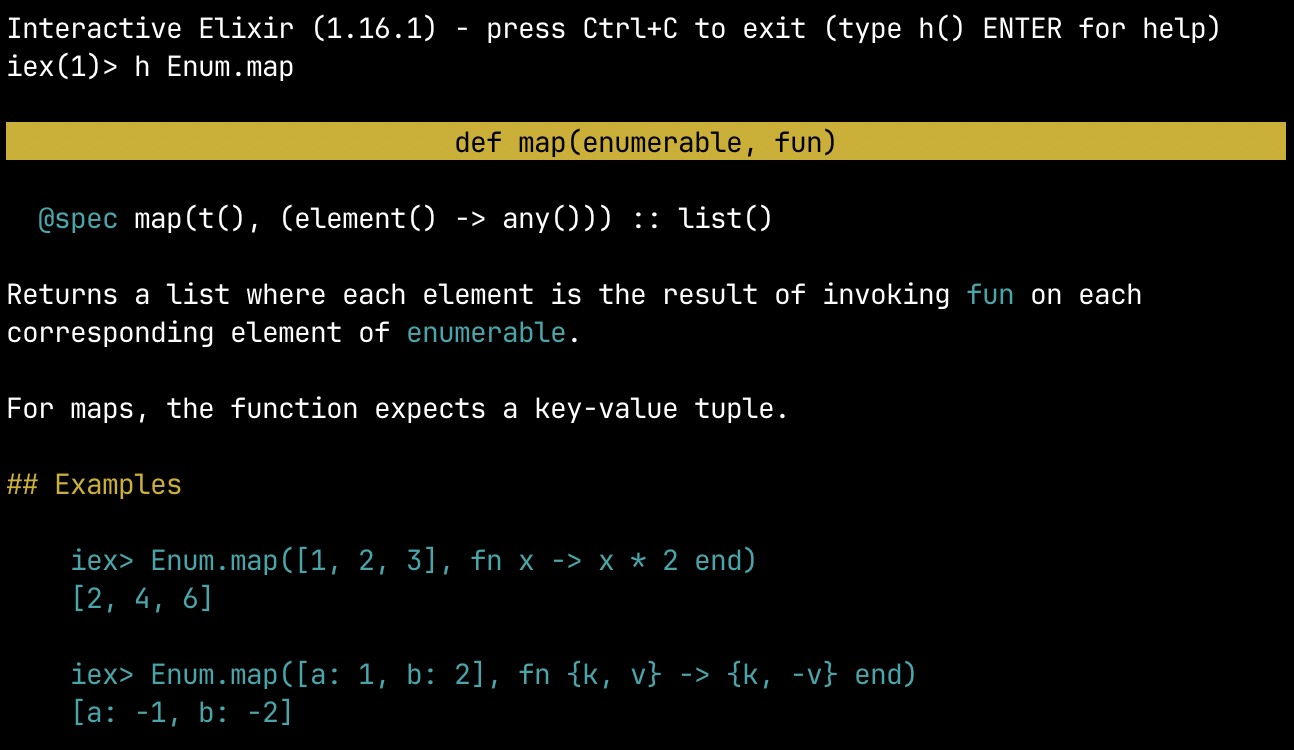
\includegraphics[width=0.8\linewidth]{1_1.png}
  % 添加标题
  \caption{交互式Elixir内置了文档}
  % 添加标签,用于引用
  \label{fig:1_1}
\end{figure}


但\texttt{iex}的功能不止于此!这个工具还允许你连接到\emph{节点},可以理解为可以互相通信的独立Erlang运行时。这些运行时可以存在于同一台计算机、同一局域网或同一网络上。

\texttt{iex}还有一个受Ruby库\texttt{Pry}启发的超能力。如果你之前用过\texttt{Pry},你会知道它是一个允许你深入程序状态的调试器。\texttt{iex}也有一个同名功能,叫做\texttt{IEx.pry}。虽然本书中我们不会使用这个功能,但这是一个非常有价值的工具。以下是如何使用它的简要概述。假设我有这样的代码:

\begin{code}{一个GenServer的示例}
\begin{minted}[linenos]{elixir}
require IEx

defmodule Greeter do
  def ohai(who, adjective) do
    greeting = "Ohai!, #{adjective} #{who}"
    # <--- 这里
    IEx.pry()
  end
end
\end{minted}
\label{lst:genserver_example}
\end{code}

\texttt{IEx.pry}这一行会使解释器暂停,允许我检查传入的变量。首先,我会运行这个函数:

\begin{code}{}\begin{minted}[linenos]{bash}

iex(1)> Greeter.ohai "leader", "glorious"
Request to pry #PID<0.62.0> at ohai.ex:6

    def ohai(who, adjective) do
        greeting = "Ohai!, #{adjective} #{who}"
        IEx.pry
    end
end

Allow? [Yn] Y
\end{minted}
% \caption{Listing Caption}
% \label{lst:id}
\end{code}

一旦我回答 \texttt{Y},我就会进入 \texttt{iex},在那里我可以开始检查传入的变量

\begin{code}{}\begin{minted}[linenos]{bash}
Interactive Elixir (1.2.4) - press Ctrl+C to exit (type h() ENTER for help)
pry(1)> who
"leader"
pry(2)> adjective
"glorious"
\end{minted}
% \caption{Listing Caption}
% \label{lst:id}
\end{code}

在使用\texttt{iex}的过程中,你还会发现其他一些不错的功能,比如\emph{自动补全}。几乎每次Elixir的更新都会给\texttt{iex}带来一些改进和额外的辅助函数,记得跟踪变更日志!

\subsection{使用ExUnit进行测试}

Elixir内置了一个测试框架,名为\texttt{ExUnit}。\texttt{ExUnit}有一些非常好的功能,比如能够\emph{异步}运行,还能产生美观的失败信息,如图1.2所示。ExUnit之所以能够在错误报告方面做出巧妙的处理,主要是因为\emph{宏},我们在本书中不会涉及这个话题。尽管如此,这仍然是一个值得探索的有趣话题。

\begin{figure}[htbp]
  \centering
  % 插入图片文件
  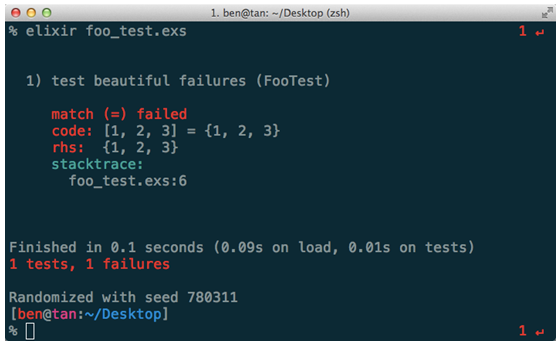
\includegraphics[width=0.8\linewidth]{1_2.png}
  % 添加标题
  \caption{ExUnit 提供了出色的错误信息}
  % 添加标签,用于引用
  \label{fig:1_2}
\end{figure}

\subsection{Mix}\label{mix}

Mix 是一个构建工具,用于创建、编译、测试 Elixir项目。它还用于管理依赖关系等。可以将其类比为 Ruby 中的\texttt{rake} 和 Clojure 中的
\texttt{lein}。事实上,一些最初为\texttt{mix} 做出贡献的开发者也参与了\texttt{lein} 的编写。例如 Phoenix 网络框架就使用 Mix来创建生成器,从而减少编写不必要的样板代码。


\subsection{标准库}

Elixir 自带了一个出色的标准库。数据结构如范围、严格和惰性枚举API,以及合理的字符串操作方式等,都是其中的亮点。

虽然 Elixir可能不是编写脚本的最佳语言,但它包含了一些听起来很熟悉的库,如\texttt{Path} 和\texttt{File}。其文档也非常易用。解释清晰、简洁,并附有如何使用各种库及其函数的示例。

Elixir 拥有一些标准 Erlang 库中没有的模块。我最喜欢的其中之一是\texttt{Stream}。流基本上是可组合的、惰性的枚举。它们通常用于模拟潜在的无限值流。

Elixir 还向 OTP 框架增加了功能。例如,它增加了许多抽象,如\texttt{Agent}来处理状态,\texttt{Task}来处理一次性异步计算。这两者都是基于默认随 OTP 提供的\texttt{GenServer}(代表\emph{通用服务器})构建的。


\subsection{元编程}

Elixir具有类似LISP的宏功能,只是没有括号。宏用于通过用现有构造表达新构造来扩展Elixir语言。语言实现在整个语言中广泛使用宏。库作者也广泛使用它来减少样板代码(Boilerplate code)。

\subsection{生态系统}

作为一种相对较新的编程语言,Elixir建立在一个坚实且经过验证的语言之上,这无疑带来了其优势。


\subsubsection{感谢你,Erlang!}

我认为Elixir最大的收获是来自Erlang社区多年的经验和工具。几乎任何Erlang库都可以轻松地在Elixir中使用。Elixir开发者不必重新发明轮子来构建坚如磐石的应用程序。相反,他们可以高兴地依赖于OTP。他们可以专注于基于现有库构建额外的抽象。


\subsubsection{学习资源}

Elixir的兴奋引发了学习资源的涌现(在这里不是自吹自擂)。已经有多个录像教程、书籍和会议。事实上,一旦你学会了从Elixir到Erlang的转换,你还将受益于众多撰写得很好的Erlang书籍,如《Learn
You Some Erlang for Great Good!》和《Designing for Scalability with
Erlang/OTP》。


\subsubsection{Phoenix}

Phoenix是用Elixir编写的网络框架,它让许多开发者感到非常兴奋,而且理由充分。首先,Phoenix的响应时间可以达到\emph{微秒级}。Phoenix证明了你可以同时拥有一个高性能且简单的框架,并且内置了对WebSockets的支持,还得到了OTP强大功能的支持。


\subsubsection{它仍在发展}

Elixir仍在不断发展和探索新想法。我所看到的最有趣的事情之一是正在研究的并发抽象。更好的是,Elixir核心团队不断寻找来自其他语言的伟大想法。如果你知道在哪里看,Elixir中已经至少有Ruby、Clojure和F\#的DNA。

\section{为什么选择 Elixir 而不是 X?}

在我做关于 Elixir 的演讲或写作时,经常会遇到这样一个问题:我应该学习
Elixir 还是\emph{X}?这里的\emph{X}通常是指 Clojure、Scala 或
Golang。这个问题通常源于两个其他问题。首先,Elixir
是否在获得关注。其次是 Elixir 工作的可用性。以下是我对这些问题的回答:

\begin{itemize}

\item  Elixir  是一种非常年轻的语言(Elixir发布于2012年,本书写作时大约有5年历史),所以它需要时间。你可以把这当作你的优势。
\item  函数式编程正在崛起。大多数函数式编程语言中都有一些或多或少相同的原则。这意味着无论是  Scala、Clojure 还是 Erlang,\emph{这些技能都是可移植的}。
\item  Erlang  似乎又开始受欢迎了。对分布式系统和物联网(IoT)的兴趣也在增加,这些都是  Elixir 的强项。
\end{itemize}

我有种直觉,Elixir 很快就会起飞。就像 Java刚出现的那些日子。最初没多少人关注它。但是,早期的采用者获得了巨大的回报。Ruby的故事也是一样。领先一步绝对有优势。

我太自私了,不能让其他人错过学习和体验这门精彩语言的机会。抛开你的疑虑,有点信心,享受这段旅程吧!


\section{Elixir/OTP有什么用?}

Erlang 所擅长的,对 Elixir 也同样适用。Elixir 和 OTP结合在一起提供了构建并发、可扩展、容错和分布式程序的设施。这些包括但显然不限于:

\begin{itemize}

\item  聊天服务器(WhatsApp, Ejabberd)
\item  游戏服务器(Wooga)
\item  网络框架(Phoenix)
\item  分布式数据库(Riak 和 CouchDB)
\item  实时竞价服务器
\item  视频流服务
\item  长期运行的服务/守护进程
\item  命令行应用程序
\end{itemize}

从这个列表中,你可能会发现 Elixir 非常适合构建服务器端软件 - 你是对的!这些软件有相似的特点。它们必须:

\begin{itemize}

\item  服务于成千上万甚至百万的用户和客户端,同时保持良好的响应水平
\item  即使在失败的情况下也能保持运行,或有优雅的故障转移机制
\item  优雅地扩展,无论是增加更多的 CPU 核心还是额外的机器
\end{itemize}

Elixir并不是万能药(双关梗)。你可能不会想用它来进行图像处理、计算密集型任务或构建GUI 应用程序。你不会用 Elixir 来构建硬实时系统。例如,你不应该用 Elixir编写 F-22 战斗机的软件。

但嘿,别让我告诉你能做什么或不能做什么用Elixir。让你的创造力流淌。这就是编程如此精彩的原因。

\section{前方的路}

现在我们已经介绍了一些关于Elixir、Erlang和OTP框架的背景知识,以下将对未来内容进行高层次的概述。

\subsection{OTP行为的预览}

假设你想要构建一个天气应用程序。你决定获得一些风险投资资金,不知不觉中,你得到了资助。

经过一番思考,你意识到你实际上要构建的是一个简单的客户端-服务器应用程序(当然,你不会告诉你的投资者这一点)。基本上,客户端(例如通过HTTP)会发出请求,你的应用程序必须执行一些计算并及时将结果返回给每个客户端。

于是,你开始实施你的天气应用程序,并将其投入生产。你的天气应用程序突然走红,用户突然遇到了各种问题,比如加载时间慢,甚至更糟,服务中断。你尝试进行一些性能分析,调整这里那里的设置,甚至尝试增加更多的并发处理。

一切看起来暂时还好,但这只是暴风雨前的平静。最终,你的用户再次遇到同样的问题,只不过这次你收到了死锁和其他奇怪错误消息的报告。最后,你放弃了,并写了一篇长篇博客文章,解释为什么你的初创企业失败,为什么你应该用Node.js或Golang来构建你的初创企业。这篇文章在Hacker News上排名第一达一个月之久。

虽然这本书不会向你展示如何获得风险投资资金,但它会向你展示如何使用OTP来构建一个天气服务,以及其他有趣的事情。OTP框架赋予了BEAM语言(Erlang、Elixir等)超能力,并在安装Elixir时捆绑在一起。

我们提到过,OTP用于构建并发、可扩展、容错和分布式程序。在OTP中,最重要的概念之一是\textbf{行为(Behavior)}的概念。行为可以被认为是你和OTP之间的一种契约。

当你使用一个行为时,OTP期望你填充某些函数。作为交换,OTP会处理一系列问题,如消息处理(实现同步或异步)、并发错误(死锁和竞态条件)、容错和失败处理。这些问题是通用的------几乎每个值得尊敬的客户端/服务器程序都必须以某种方式处理它们,而OTP介入并为你处理所有这些。此外,这些通用部分已在生产中使用,并经过多年的实战测试。

在本书中,我们将使用两种最常用的\textbf{行为}:\texttt{GenServer}和\texttt{Supervisor}。当然还有其他行为。一旦你习惯了学习如何使用上述行为,使用其他行为就会变得相当直接。

虽然你完全可以自己实现一个Supervisor行为,但$99.999999999\%$的时间里没有好的理由这样做。实施者们已经深思熟虑了大多数客户端-服务器程序需要包含的功能,并且还考虑了并发错误和各种边缘情况。你如何使用OTP行为?以下是使用GenServer行为的天气服务的最小实现:

\begin{code}{}\begin{minted}[linenos]{elixir}
defmodule WeatherService do
  # <- 引入了GenServer行为 (GenServer behaviour)
  use GenServer

  # 这是一个同步请求
  def handle_call({:temperature, city}, _from, state) do
    # ...
  end

  # 这是一个异步请求
  def handle_cast({:email_weather_report, email}, state) do
    # ...
  end
end
\end{minted}
\end{code}

虽然上面的实现显然不完整,但重要的是要意识到(你在阅读本书时会看到)哪些事情是\emph{不需要}做的。例如,你不必实现如何处理同步或异步请求的具体方式。我现在先不剧透(毕竟这只是一个预览),但我们会分别构建不使用OTP和使用OTP的相同应用程序。

一开始,OTP可能看起来非常复杂和可怕,但当你在书中逐个例子学习时,你会发现事实并非如此。

\emph{了解某样东西如何工作最好的方式就是亲自实现它}。本着这种精神,你将学习如何从零开始实现监督者行为(Supervisor
behaviour)。这样做的目的是为了展示其实并没有太多神奇之处,只是该语言提供了构建这些有用抽象的必要工具。

我们还将从头开始实现一个工作池应用程序,并逐步发展它。这基于前面的GenServer和监督者章节。

\subsection{分布式负载均衡和容错}

Elixir和OTP是构建分布式系统的绝佳选择。在本书中,我们将构建\emph{两个}不同用途的分布式应用程序。

一个创建分布式应用程序的原因是将负载分散到多台计算机上。你将创建一个负载测试器,并了解如何利用分布式处理来扩展应用程序的能力。

你将看到,由于Elixir的消息传递导向性质和可用的分布式原语,与其他语言和平台相比,构建分布式应用程序会是一种更加愉快的体验。

另一个需要分布式的原因是为了\emph{容错}。如果一个节点失败,你会希望另一个节点能代替它。你也将了解如何创建这样的应用程序。

\subsection{使用Dialyzer和类型规范}

由于Elixir是一种动态语言,我们需要警惕在程序中引入类型错误。因此,确保类型安全是可靠性的一个方面。

Dialyzer是OTP中的一个工具,旨在检测这些问题中的一些。你将通过一系列示例学习如何使用Dialyzer。你还将了解Dialyzer的局限性。

最后,你将看到如何通过使用类型规范来帮助Dialyzer克服这些局限性。你还将学习到,除了帮助Dialyzer,类型规范也可作为文档。例如,以下摘自List模块:

\begin{code}{一个使用类型规范注解的函数示例}
\begin{minted}[linenos]{elixir}
@spec foldl([elem], acc, (elem, acc -> acc)) :: acc when elem: var, acc: var
def foldl(list, acc, function) when is_list(list) and is_function(function) do
  :lists.foldl(function, acc, list)
end
\end{minted}
\label{lst:list_docstr}
\end{code}

在学习了Dialyzer(类型检查器)和类型规范之后,你将会开始欣赏类型规范,以及它们如何帮助使你的程序更清晰、更安全。

\subsection{属性和并发测试}

最后两章专门讲述基于属性的测试和并发测试。特别是,我们将学习如何使用QuickCheck(快速检查工具)和Concuerror(并发错误检测工具)。这两个工具不是 Elixir 或 OTP默认提供的。然而,这两种工具在揭示传统单元测试工具无法发现的错误方面非常有用。

我们将学习 QuickCheck以进行基于属性的测试,并了解基于属性的测试是如何颠覆传统单元测试的。与单元测试中考虑特定示例不同,基于属性的测试迫使你提出应该适用于你测试代码的一般性属性。一旦你创建了一个属性,就可以针对成百上千个\emph{生成的}测试输入进行测试。这里有一个示例,说明两次反转列表会得到相同的列表:

\begin{code}{一个属性测试的示例}
\begin{minted}[linenos]{elixir}
@tag numtests: 100
property "reverse is idempotent" do
  forall l <- list(char) do
    ensure(l |> Enum.reverse() |> Enum.reverse() == l)
  end
end
\end{minted}
\label{lst:property_test_example}
\end{code}

这将生成一百个列表,并断言上述属性对每个生成的列表都成立。

我们将要探索的另一个工具是 Concuerror。Concuerror是一个源于学术界但已在现实世界中得到应用的工具。我们将学习 Concuerror是如何揭示难以检测的并发错误,如死锁和竞态条件的。通过一系列故意含有错误的示例,你将使用Concuerror 来揭示这些错误。

\section{总结}

在本章中,我们探讨了Erlang创建的动机,以及它如何完美地适应我们今天的多核心和网络规模现象。然后,我们了解了Elixir的动机,并提出了几个为什么Elixir比Erlang更好的理由,例如Elixir的标准库和工具链。我们还看了一些完美适用于Elixir和OTP的示例。

本章的另一半提供了即将到来内容的概览。我们以OTP的简要介绍和使用OTP实现天气服务的预览开始。然后,我们讨论了负载均衡和分布式的分布。如你将很快看到,Elixir和OTP提供的分布式原语使编写分布式程序比你可能使用的其他语言容易得多。最后,我们探索了一些帮助使你的代码更可靠的工具,即Dialyzer、QuickCheck和Concuerror。

在下一章中,我们将迅速开始学习Elixir的语言特性。你将学习核心数据类型、模式匹配、递归、编写函数等!

\chapter{快速入门}\label{chapt:tour}

本章内容包括:

\begin{itemize}

\item 第一个Elixir程序
\item 使用交互式Elixir(iex)
\item 数据类型
\item 模式匹配
\item 列表与递归
\item 模块与函数
\item 管道(\texttt{|>})运算符
\item Erlang互操作性
\end{itemize}

我认为,与其深入每个语言特性,不如通过一系列示例来呈现它们。对于Java或Ruby程序员来说可能陌生的概念,我会进行更多的阐述。对于某些概念,您可能可以从您已知的任何语言中找到相似之处。这些示例会逐渐变得更有趣,几乎展示了理解本书中Elixir代码所需的所有内容。

\section{设置环境}

Elixir在所有主流编辑器上都得到了很好的支持,比如Vim、Emacs、Spacemacs、Atom、IntelliJ和VisualStudio。例如,专门为Emacs/Spacemacs与Elixir集成开发的Alchemist\pagenote{https://github.com/tonini/alchemist.el},提供了极佳的开发体验。它具有诸如文档查找、智能代码补全、与\texttt{iex}和\texttt{mix}的集成等众多有用的功能。与其他编辑器集成相比,它是支持最广泛、功能最丰富的。

准备好你的终端和编辑器,因为快速入门之旅现在就开始。

\section{第一步}

让我们从简单的开始。由于我曾经的殖民统治者(我来自新加坡),我对英尺、英寸及其亲戚们的度量单位不太熟悉。我们将编写一个长度转换器来解决这个问题。

以下是我们如何在Elixir中定义长度转换器的方法。输入以下内容到你最喜欢的文本编辑器中,并将文件保存为\texttt{length\_converter.ex}。

\begin{code}{Elixir中的长度转换程序}
\begin{minted}[linenos]{elixir}
defmodule MeterToFootConverter do
  def convert(m) do
    m * 3.28084
  end
end
\end{minted}
\label{lst:length_converter}
\end{code}

\texttt{defmodule} 定义一个新模块(即\texttt{MeterToFootConverter}),而\texttt{def} 定义一个新函数(即\texttt{convert})。

\subsection{在交互式Elixir中运行Elixir程序}

交互式Elixir,或简称\texttt{iex},相当于Ruby中的\texttt{irb} 或NodeJS中的\texttt{node}。在你的终端中,使用文件名作为参数启动\texttt{iex}。

\begin{code}{运行长度转换程序(\texttt{iex})}
\centering
\begin{minted}[linenos]{elixir}
% iex length_converter.ex
Erlang/OTP 26 [erts-14.2.1] [source] [64-bit] [smp:8:8] [ds:8:8:10] [async-threads:1] [jit] [dtrace]

Interactive Elixir (1.16.1) - press Ctrl+C to exit (type h() ENTER for help)
iex(1)>
\end{minted}
\label{lst:2-2}
\end{code}

世界上最高的男人的记录是2.72米。那是多少英尺?让我们找出答案:

\begin{code}{}
\begin{minted}[linenos]{elixir}
iex(1) > MeterToFootConverter.convert(2.72)
\end{minted}
% \label{lst:id}
\end{code}

结果是

\begin{code}{}
\begin{minted}[linenos]{elixir}
8.9238848
\end{minted}
% \label{lst:id}
\end{code}

\subsection{停止Elixir程序}

有几种方法可以停止Elixir程序,或者如果你想退出iex。第一种方法是输入\texttt{Ctrl + C}。第一次这样做时,你会看到:

\begin{code}{在iex中停止运行的Elixir程序}
\begin{minted}[linenos]{bash}
BREAK: (a)bort (A)bort with dump (c)ontinue (p)roc info (i)nfo
       (l)oaded (v)ersion (k)ill (D)b-tables (d)istribution
\end{minted}
\label{lst:stop_elixir_program}
\end{code}

你可以选择 \texttt{a)} 输入 \texttt{a}来中止,或者再次输入\texttt{Ctrl + C}。
另一种选择是使用\texttt{System.halt},虽然我个人更喜欢\texttt{Ctrl + C}。

\subsection{获取帮助}

由于\texttt{iex}是与Elixir交互的主要工具,因此学习更多关于它的信息是很有价值的。特别是,\texttt{iex}有一个非常棒的内置文档系统。再次启动\texttt{iex}。假设你想了解\texttt{Dict} 模块。你可以在\texttt{iex} 中输入\texttt{h Dict},输出将类似于图\ref{fig:2_3}。

\begin{figure}[!ht]
    \centering
    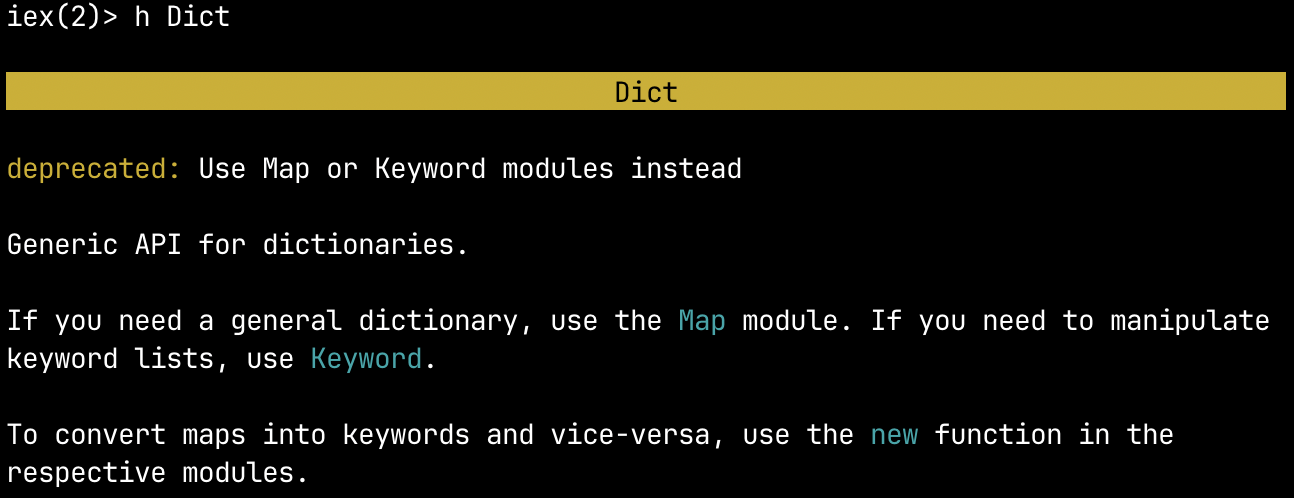
\includegraphics[width=0.8\linewidth]{2_3.png}
    \caption{在iex中显示的Dict模块文档}
    \label{fig:2_3}
\end{figure}


\texttt{Dict} 有哪些可用的函数?输入\texttt{Dict.}(重要的是后面的点\texttt{.}!),然后按你的\texttt{<Tab>} 键。你将看到\texttt{Dict} 模块中可用的函数列表,如图\ref{fig:2_4}所示。

\begin{figure}[!ht]
    \centering
    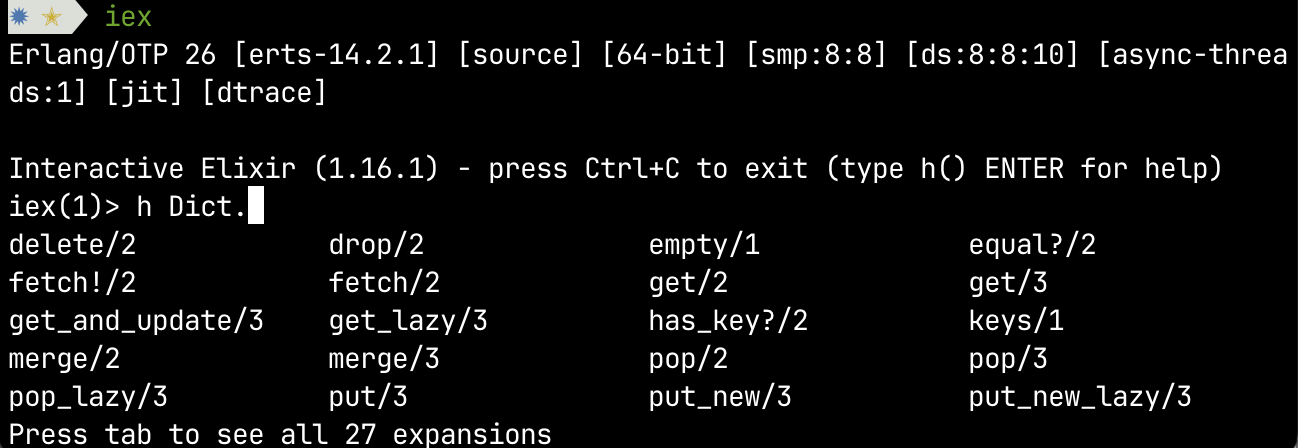
\includegraphics[width=0.8\linewidth]{2_4.png}
    \caption{\texttt{Dict} 模块中可用的函数列表}
    \label{fig:2_4}
\end{figure}


现在,假设你想了解更多关于 \texttt{put/3}函数。我稍后会解释 \texttt{/3}是什么意思。现在,它只意味着这个版本的 \texttt{put}接受3个参数。在 \texttt{iex} 中,输入\texttt{h Dict.put/3}。输出看起来像图\ref{fig:2_5}:

\begin{figure}[!ht]
    \centering
    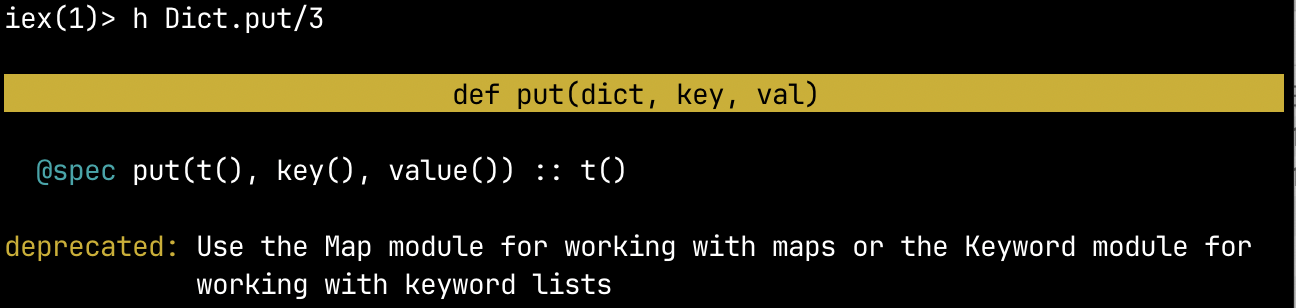
\includegraphics[width=0.8\linewidth]{2_5.png}
    \caption{\texttt{Dict.put/3} 的文档}
    \label{fig:2_5}
\end{figure}


相当整洁,对吧?更好的是,文档还有美观的语法高亮。

\begin{quote}
\textbf{注意}:因为本书成书较早,有许多内容已经过时。例如,你会注意到\texttt{h Dict}的输出中显示了deprecated的字样,表明该模块已被弃用。这是因为在Elixir 1.11中,\texttt{Dict}模块已被弃用。在Elixir1.11中,你应该使用\texttt{Map}模块。
\end{quote}

\section{数据类型}

在本书中,我们将使用以下常见数据类型:

\begin{itemize}

\item  模块(Modules)
\item  函数(Functions)
\item  数字(Numbers)
\item  字符串(Strings)
\item  原子(Atoms)
\item  元组(Tuples)
\item  映射(Maps)
\end{itemize}

\subsection{模块、函数和函数子句}

模块是Elixir用于将函数组合在一起的方式。模块的例子包括\texttt{List}、\texttt{String},当然还有\texttt{MeterToFootConverter}。使用\texttt{defmodule}创建模块。同样,使用\texttt{def}创建函数。


\subsubsection{模块}

让我们编写另一个函数,将米转换为\emph{英寸}。根据我们当前的实现,我们需要做一些更改。首先,我们的模块名太具体了。让我们将其更改为更通用的名称: \texttt{length\_converter.ex}。我们如何添加一个将米转换为英寸的函数?这是一种\emph{可能的}方法:


\begin{code}{\texttt{defmodules}可以嵌套}
\begin{minted}[linenos]{elixir}
defmodule MeterToLengthConverter do
  defmodule Feet do
    def convert(m) do
      m * 3.28084
    end
  end

  defmodule Inch do
    def convert(m) do
      m * 39.3701
    end
  end
end
\end{minted}
\label{lst:defmodules_can_be_nested}
\end{code}

现在,您可以计算最高的男人的身高(以英寸为单位):

\begin{code}{使用点表示法(\texttt{iex})}
\begin{minted}[linenos]{elixir}
iex > MeterToLengthConverter.Inch.convert(2.72)
\end{minted}
\label{lst:use_dot_notation}
\end{code}

返回\texttt{107.08667200000001}。这个例子说明了模块可以嵌套。这里,模块\texttt{Feet}和\texttt{Inch}嵌套在\texttt{MeterToLengthConverter}内。要访问嵌套模块中的函数,使用\emph{点表示法}。通常,要在Elixir中调用函数,使用以下格式:

\begin{code}{扁平化模块层次结构(\texttt{iex})}
\begin{minted}[linenos]{elixir}
Module.function(arg1, arg2, ...)
\end{minted}
\label{lst:flatten_module_hierarchy}
\end{code}

在邮件列表中,这有时被称为``\textbf{MFA}''。它代表\textbf{模块(Module)}、\textbf{函数(Function)}和\textbf{参数(Arguments)}。记住这种格式,因为您将在本书中再次遇到它。

您还可以像这样扁平化模块层次结构:

\begin{code}{}\begin{minted}[linenos]{elixir}
# 1
defmodule MeterToLengthConverter.Feet do
  def convert(m) do
    m * 3.28084
  end
end

# 1
defmodule MeterToLengthConverter.Inch do
  def convert(m) do
    m * 39.3701
  end
end

# 1 您可以使用点表示法来指定嵌套层次结构
\end{minted}
\end{code}


您将以与代码\ref{lst:use_dot_notation} 完全相同的方式调用该函数。


\subsubsection{函数和函数子句}

编写长度转换器的更习惯的方式是使用函数子句。这是我们长度转换器的修订版本:

\begin{code}{函数子句版本的长度转换器}
\begin{minted}[linenos]{elixir}
defmodule MeterToLengthConverter do
  def convert(:feet, m) do
    m * 3.28084
  end

  def convert(:inch, m) do
    m * 39.3701
  end
end
\end{minted}
\label{lst:function_clause_version_of_length_converter}
\end{code}

定义一个函数相当直接。大多数函数都是这样写的:

\begin{code}{函数的例子}
\begin{minted}[linenos]{elixir}
def convert(:feet, m) do
  m * 3.28084
end
\end{minted}
\label{lst:function_example}
\end{code}

单行函数这样写:

\begin{code}{单行函数}
\begin{minted}[linenos]{elixir}
def convert(:feet, m), do: m * 3.28084
\end{minted}
\label{lst:single_line_function}
\end{code}

既然我们提到了,让我们再添加一个将\emph{米}转换为\emph{码}的函数,这次使用单行变体:

\begin{code}{\texttt{length\_converter}的单行函数变体}
\begin{minted}[linenos]{elixir}
defmodule MeterToLengthConverter do
  def convert(:feet, m), do: m * 3.28084
  def convert(:inch, m), do: m * 39.3701
  def convert(:yard, m), do: m * 1.09361
end
\end{minted}
\label{lst:length_converter_single_line_function_variant}
\end{code}

函数按其\emph{元数}(它接受的参数数量)来引用。因此,我们将上述函数称为\texttt{convert/2}。\texttt{convert/2}是\emph{命名函数}的一个例子。Elixir还有\emph{匿名函数}的概念。这是一个匿名函数的常见例子:

\begin{code}{第二个参数是一个匿名函数(\texttt{iex})}
\begin{minted}[linenos]{elixir}
iex > Enum.map([1, 2, 3], fn x -> x * x end)
\end{minted}
\label{lst:second_argument_is_an_anonymous_function}
\end{code}

给出\texttt{[1, 4, 9]}

我们可以定义具有相同名称的多个函数,就像我们的示例中那样。需要注意的重要一点是它们\emph{必须}被分组在一起。因此,下面是一个错误示范:

\begin{code}{始终将相似的函数子句分组在一起}
\begin{minted}[linenos]{elixir}
defmodule MeterToLengthConverter do
  def convert(:feet, m), do: m * 3.28084
  def convert(:inch, m), do: m * 39.3701
  # 1
  def i_should_not_be_here, do: IO.puts("Oops")
  def convert(:yard, m), do: m * 1.09361
end

# 1 不要这样做!
\end{minted}
\label{lst:always_group_similar_function_clauses}
\end{code}


Elixir会相应地抱怨:
\begin{code}{当函数子句未分组在一起时,Elixir会抱怨}
\begin{minted}[linenos]{bash}
% iex length_converter.ex
    warning: clauses with the same name and arity (number of arguments) should be grouped together, "def convert/2" was previously defined (length_converter.ex:2)
    │
  5 │   def convert(:yard, m), do: m * 1.09361
    │       ~
    │
    └─ length_converter.ex:5:7
\end{minted}
\label{lst:elixir_complains_when_function_clauses_are_not_grouped_together}
\end{code}

另一个重要的事情:顺序很重要。每个函数子句都是自上而下匹配的。这意味着一旦Elixir找到一个兼容的函数子句匹配,它就会停止搜索并执行该函数。对于我们当前的长度转换器,移动函数子句不会影响任何事情。当我们稍后探讨递归时,您将开始理解函数子句顺序为何重要。

\subsection{数字(Numbers)}

在 Elixir 中,数字的运作方式和传统编程语言中的类似。

\begin{code}{操作整数、十六进制数和浮点数}
\begin{minted}[linenos]{elixir}
iex(1) > 1 + 0x2F / 3.0
16.666666666666664
\end{minted}
\label{lst:operating_on_integers_hexadecimal_numbers_and_floats}
\end{code}

\begin{code}{除法和余数函数}
\begin{minted}[linenos]{elixir}
iex(1) > div(10, 3)
3

iex(2) > rem(10, 3)
1
\end{minted}
\label{lst:dif_and_rem_functions}
\end{code}

\subsection{字符串(Strings)}

Elixir中的字符串有两种形态。表面上看,字符串看起来很标准。这里有一个展示字符串插值的例子:

\begin{code}{Elixir 支持字符串插值}
\begin{minted}[linenos]{elixir}
iex(1) > "字符串是 #{:great}!"
\end{minted}
\label{lst:elixir_supports_string_interpolation}
\end{code}

将给出:

\begin{code}{对字符串的操作}
\begin{minted}[linenos]{elixir}
"字符串是 great!"
\end{minted}
% \caption{Listing Caption}
% \label{lst:id}
\end{code}

我们还可以对字符串执行各种操作:

\begin{code}{}\begin{minted}[linenos]{elixir}
iex(2) > "字符串是 #{:great}!" |> String.upcase() |> String.reverse()
\end{minted}
% \label{lst:operating_on_strings}
\end{code}

这将返回:

\begin{code}{字符串是二进制数据}
\begin{minted}[linenos]{elixir}
"!TAERG 是串符字"
\end{minted}
% \caption{Listing Caption}
% \label{lst:id}
\end{code}


\subsubsection{字符串是二进制数据(Binaries)。}

如何测试一个字符串?没有 \texttt{is\_string/1}函数可用。这是因为在 Elixir中,字符串是一种\textbf{二进制数据}。二进制数据只是一个字节序列。

\begin{code}{}\begin{minted}[linenos]{elixir}
iex(3) > "字符串是二进制数据" |> is_binary
\end{minted}
% \label{lst:strings_are_binaries}
\end{code}

返回\texttt{true}。

展示字符串的二进制表示的一种方式是使用二进制串联运算符\texttt{<>}来附加一个空字节,\texttt{<<0>>}:

\begin{code}{展示字符串的二进制表示}
\begin{minted}[linenos]{elixir}
iex(4) > "ohai" <> <<0>>
\end{minted}
\label{lst:showing_the_binary_representation_of_a_string}
\end{code}

返回 \mintinline{elixir}|<<111, 104, 97, 105, 0>>|

每个数字代表一个字符:

\begin{code}{字符串不是字符列表}
\begin{minted}[linenos]{elixir}
iex(5) > ?o
111
iex(6) > ?h
104
iex(7) > ?a
97
iex(8) > ?i
105
\end{minted}
% \caption{Listing Caption}
% \label{lst:id}
\end{code}

为了进一步确信二进制表示与原字符串等价:

\begin{code}{}\begin{minted}[linenos]{elixir}
iex(44) > IO.puts(<<111, 104, 97, 105>>)
\end{minted}
% \caption{Listing Caption}
% \label{lst:id}
\end{code}

将给你原始字符串:

\begin{code}{}\begin{minted}[linenos]{elixir}
ohai
:ok
\end{minted}
% \caption{Listing Caption}
% \label{lst:id}
\end{code}


\subsubsection{字符串不是字符列表(Char lists)}

顾名思义,字符列表是字符的列表。它与字符串是完全不同的数据类型,这可能会有些混淆。虽然字符串总是用双引号括起来,字符列表则用单引号括起来。

\begin{code}{}\begin{minted}[linenos]{elixir}
iex(9) > ~c"ohai" == "ohai"
\end{minted}
% \label{lst:strings_are_not_char_lists}
\end{code}

将给出 \texttt{false}。你通常不会使用字符列表,至少在Elixir 中不会。然而,当与某些 Erlang库交互时,你可能需要这样做。例如,在后面的示例中,Erlang 的 http客户端(httpc)接受字符列表作为 URL:\mintinline{elixir}|:httpc.request 'http://www.elixir-lang.org'|
如果我们传入字符串(二进制数据)会发生什么呢?试试看:

\begin{code}{:httpc.request/1 期望 URL 类型为字符列表}
\begin{minted}[linenos]{elixir}
iex(51)> :httpc.request "http://www.elixir-lang.org"
** (ArgumentError) 
:erlang.tl("http://www.elixir-lang.org")
(inets) inets_regexp.erl:80: :inets_regexp.first_match/3
(inets) inets_regexp.erl:68: :inets_regexp.first_match/2
(inets) http_uri.erl:186: :http_uri.split_uri/5
(inets) http_uri.erl:136: :http_uri.parse_scheme/2
(inets) http_uri.e

l:88: :http_uri.parse/2
(inets) httpc.erl:162: :httpc.request/5
\end{minted}
\label{lst:httpc_request_1_expects_the_url_to_be_a_char_list}
\end{code}


我们将在本章后面进一步讨论调用 Erlang 库的内容,但当你处理某些 Erlang库时,这是你需要记住的事情。

 \subsection{原子 (Atoms)}

原子在Elixir中作为常量存在,有点类似于Ruby中的符号。原子总是以冒号开始。创建原子有两种不同的方式:\texttt{:hello\_atom}和\texttt{:"Hello Atom"}都是有效的原子。需要注意的是,原子和字符串并不相同,因为原子和字符串是完全不同的数据类型。

\begin{code}{原子不是字符串}
\begin{minted}[linenos]{elixir}
iex > :hello_atom == "hello_atom"
false
\end{minted}
\label{lst:atoms_are_not_strings}
\end{code}

单独来看,原子并不是非常有趣。然而,当我们将原子放入\emph{元组}中,并在\emph{模式匹配}的上下文中使用它们时,你就会开始理解原子的作用以及Elixir如何利用原子编写声明性代码。我们将在后面几节中讨论模式匹配。现在,让我们转向元组。

 \subsection{元组 (Tuples)}

一个元组可以包含不同类型的数据。例如,一个HTTP客户端可能以元组的形式返回一个成功的请求:
\mintinline{elixir}|{200, "http://www.elixir-lang.org"}|
一个失败的请求可能看起来像这样:
\mintinline{elixir}|{404, "http://www.php-is-awesome.org"}|

元组使用基于零的访问方式,就像在大多数编程语言中访问数组元素一样。因此,如果你想要获取请求结果的URL,你需要传入\texttt{1}给\texttt{elem/2}:

\begin{code}{访问元组中的第二个元素}
\begin{minted}[linenos]{elixir}
iex > elem({404, "http://www.php-is-awesome.org"}, 1)
\end{minted}
\label{lst:accessing_the_second_element_of_a_tuple}
\end{code}

这将返回 \texttt{http://www.php-is-awesome.org}。
你可以使用\texttt{put\_elem/3}来更新一个元组:

\begin{code}{更新一个元组}
\begin{minted}[linenos]{elixir}
iex > put_elem({404, "http://www.php-is-awesome.org"}, 0, 503)
\end{minted}
\label{lst:update_a_tuple}
\end{code}

返回 \mintinline{elixir}|{503, "http://www.php-is-awesome.org"}|

\subsection{映射 (Maps)}

映射本质上是键值对,类似于哈希或字典,具体取决于你所使用的语言。所有映射操作都通过\texttt{Map}模块暴露。

使用映射相当直接,但需要注意一个小问题。看看你是否能在例子中发现它。让我们从一个空映射开始:

\begin{code}{创建一个新的映射}
\begin{minted}[linenos]{elixir}
iex > programmers = Map.new()
%{}
\end{minted}
\label{lst:create_a_new_map}
\end{code}

让我们向映射中添加一些聪明的人:

\begin{code}{向映射中添加元素}
\begin{minted}[linenos]{elixir}
iex > programmers = Map.put(programmers, :joe, "Erlang")
%{joe: "Erlang"}
iex > programmers = Map.put(programmers, :matz, "Ruby")
%{joe: "Erlang", matz: "Ruby"}
iex > programmers = Map.put(programmers, :rich, "Clojure")
%{joe: "Erlang", matz: "Ruby", rich: "Clojure"}
\end{minted}
\label{lst:add_elements_to_a_map}
\end{code}

\textbf{一个非常重要的旁白:不可变性 (Immutability)}

注意到\texttt{programmers}是\texttt{Map.put/3}的一个参数,并且\emph{重新绑定}到\texttt{programmers}上。为什么会这样?

\begin{code}{为额外检查添加守卫}
\begin{minted}[linenos]{elixir}
iex > Map.put(programmers, :rasmus, "PHP")
%{joe: "Erlang", matz: "Ruby", rasmus: "PHP", rich: "Clojure"}
\end{minted}
\label{lst:adding_guards_for_extra_checks}
\end{code}

返回值包含了新的条目。让我们检查一下\texttt{programmers}的内容:

\begin{code}{}\begin{minted}[linenos]{elixir}
iex > programmers
%{joe: "Erlang", matz: "Ruby", rich: "Clojure"}
\end{minted}
% \caption{Listing Caption}
% \label{lst:id}
\end{code}

这个属性被称为\textbf{不可变性}。

Elixir中的\textbf{所有}数据结构都是不可变的,这意味着你无法对其进行任何修改。你所做的任何修改\textbf{总是}保留原始结构\textbf{不变}。相反,返回一个修改过的副本。因此,为了捕获结果,你可以将其重新绑定到同一个变量名,或者将值绑定到另一个变量上。

\section{守卫(Guards)}

让我们再次看看
\texttt{length\_converter.ex}。假设我想确保参数始终是数字。我们可以通过添加守卫子句来修改程序:

\begin{code}{}\begin{minted}[linenos]{elixir}
defmodule MeterToLengthConverter do
  def convert(:feet, m) when is_number(m), do: m * 3.28084 #1
  def convert(:inch, m) when is_number(m), do: m * 39.3701 #1
  def convert(:yard, m) when is_number(m), do: m * 1.09361 #1
end
\#1 在函数子句中添加守卫。
\end{minted}
% \label{lst:id}
\end{code}


所以现在,如果你尝试像\mintinline{elixir}|{MeterToLengthConverter.convert(:feet, "smelly")}|这样有趣的事情,没有任何函数子句会匹配。实际上,Elixir会抛出一个\texttt{FunctionClauseError}:

\begin{code}{尝试执行上述代码会导致 FunctionClauseError}
\begin{minted}[linenos]{elixir}
iex(1)> MeterToLengthConverter.convert (:feet, "smelly")
** (FunctionClauseError) no function clause matching in MeterToLengthConverter.convert/2

    The following arguments were given to MeterToLengthConverter.convert/2:

        # 1
        :feet

        # 2
        "smelly"

    length_converter.ex:2: MeterToLengthConverter.convert/2
    iex:1: (file)
\end{minted}
\label{lst:trying_to_execute_the_above_code_will_result_in_a_functionclauseerror}
\end{code}

负长度没有意义。让我们确保参数是非负的。我们可以通过添加另一个守卫表达式来实现这一点:

\begin{code}{我们可以在守卫中包含简单表达式}
\begin{minted}[linenos]{elixir}
defmodule MeterToLengthConverter do
  # 1
  def convert(:feet, m) when is_number(m) and m >= 0, do: m * 3.28084
  # 1
  def convert(:inch, m) when is_number(m) and m >= 0, do: m * 39.3701
  # 1
  def convert(:yard, m) when is_number(m) and m >= 0, do: m * 1.09361
end

# 1 检查 m 是否为非负数
\end{minted}
\label{lst:we_can_include_simple_expressions_in_guards}
\end{code}


除了\texttt{is\_number/1},当你需要区分不同的数据类型时,还有其他类似的函数会派上用场。要生成这个列表,启动\texttt{iex},然后输入 \texttt{is\_}后跟 \texttt{<Tab>} 键。

\begin{code}{在 iex 中使用自动补全来发现函数名称}
\begin{minted}[linenos]{elixir}
iex(1)> is_
is_atom/1         is_binary/1       is_bitstring/1    is_boolean/1
is_exception/1    is_exception/2    is_float/1        is_function/1
is_function/2     is_integer/1      is_list/1         is_map/1
is_map_key/2      is_nil/1          is_number/1       is_pid/1
is_port/1         is_reference/1    is_struct/1       is_struct/2
Press tab to see all 21 expansions
\end{minted}
\label{lst:using_autocompletion_in_iex_to_discover_function_names}
\end{code}

\texttt{is\_*} 函数应该是非常直观的,除了\texttt{is\_port/1} 和\texttt{is\_reference/1}。我们在这本书中不会使用端口。稍后我们会遇到引用,你将看到它们在为消息赋予唯一身份时是如何有用的。

守卫子句在消除条件语句方面特别有用,正如你所猜测的,它们在确保你的参数是正确类型时也很有用。

\section{模式匹配}

模式匹配是函数式编程语言中最强大的功能之一,而Elixir也不例外。事实上,模式匹配是我最喜欢的Elixir功能之一。一旦你看到模式匹配能做什么,你就会开始渴望在不支持它们的语言中使用它们。

Elixir使用等号(\texttt{=})来执行模式匹配。与大多数语言不同,Elixir不仅使用\texttt{=}操作符进行变量赋值。事实上,\texttt{=}被称为\emph{匹配操作符}。从现在开始,当你看到一个\texttt{=}时,不要想它是等于,而是匹配。我们究竟在匹配什么呢?简而言之,模式匹配用于匹配值和数据结构。在接下来的示例中,你将了解为什么\texttt{=}被称为匹配操作符。更重要的是,你将学会爱上模式匹配,作为一种生成优美代码的强大工具。首先,让我们学习规则:


\subsection{\texttt{=}用于赋值}

匹配操作符的第一个规则是:变量赋值仅在变量位于表达式的\emph{左}侧时发生。

\begin{code}{变量赋值仅在变量位于左侧时发生}
\begin{minted}[linenos]{elixir}
iex > programmers = Map.put(programmers, :jose, "Elixir")
\end{minted}
\label{lst:variable_assignment_only_happens_when_the_variable_is_on_the_left}
\end{code}

将产生:
\texttt{\%\{joe: "Erlang", jose: "Elixir", matz: "Ruby", rich: "Clojure"\}}

这里,我们将\texttt{Map.put/2}的结果赋值给了\texttt{programmers}。预期中,\texttt{programmers}包含:

\begin{code}{}
\begin{minted}[linenos]{elixir}
iex > programmers
%{joe: "Erlang", jose: "Elixir", matz: "Ruby", rich: "Clojure"}
\end{minted}
% \label{lst:id}
\end{code}


\subsection{\texttt{=}也用于匹配}

现在事情变得稍微有趣一些。让我们交换一下我们之前的表达式顺序:

\begin{code}{匹配Map(在左侧)与\texttt{programmers}}
\begin{minted}[linenos]{elixir}
iex > %{joe: "Erlang", jose: "Elixir", matz: "Ruby", rich: "Clojure"} = programmers
%{joe: "Erlang", jose: "Elixir", matz: "Ruby", rich: "Clojure"}
\end{minted}
\label{lst:match_a_map_against_programmers}
\end{code}

在这里,我们调换了顺序。注意这\emph{不是}一个赋值。相反,发生了一次\emph{成功的模式匹配},因为左侧的内容和\texttt{programmers}是相同的。让我们看一个\emph{不成功}的模式匹配:

\begin{code}{一个不成功的模式匹配}
\begin{minted}[linenos]{elixir}
iex> %{tolkien: "Elvish"} = programmers
** (MatchError) no match of right hand side value: %{joe: "Erlang", jose: "Elixir", matz: "Ruby", rich: "Clojure"}
\end{minted}
\label{lst:an_unsuccessful_pattern_match}
\end{code}
当一个不成功的匹配发生时,会抛出一个\texttt{MatchError}。

\subsection{解构}
接下来我们来看看解构,因为我们需要用到它来执行一些模式匹配的酷炫技巧。
解构是模式匹配发挥作用的地方。\emph{the Common Lisp Language}\pagenote{http://www.cs.cmu.edu/Groups/AI/html/cltl/clm/node252.html}中对解构的定义是:

\emph{解构允许你将一组变量绑定到相应的值集合,这可以在任何你能将一个值绑定到单个变量的地方进行。}

用代码来解释的话:

\begin{code}{将左侧的变量绑定到右侧的值}
\begin{minted}[linenos]{elixir}
iex > %{joe: a, jose: b, matz: c, rich: d} =
  %{joe: "Erlang", jose: "Elixir", matz: "Ruby", rich: "Clojure"}
\end{minted}
\label{lst:bind_the_variables_on_the_left_to_the_values_on_the_right}
\end{code}

下面是每个变量的内容:

\begin{code}{仅匹配部分模式}
\begin{minted}[linenos]{elixir}
iex > a
"Erlang"
iex > b
"Elixir"
iex > c
"Ruby"
iex > d
"Clojure"
\end{minted}
% \caption{Listing Caption}
% \label{lst:id}
\end{code}

这里,我们将一组\emph{变量}(\texttt{a}、\texttt{b}、\texttt{c}和 \texttt{d})绑定到相应的一组\emph{值}(\texttt{Erlang}、\texttt{Elixir}、\texttt{ Ruby }和\texttt{Clojure})。如果你只对提取部分信息感兴趣怎么办?没问题,因为你可以进行模式匹配,而不需要指定整个模式:

\begin{code}{}\begin{minted}[linenos]{elixir}
iex > %{jose: most_awesome_language} = programmers
%{joe: "Erlang", jose: "Elixir", matz: "Ruby", rich: "Clojure"}
iex > most_awesome_language
"Elixir"
\end{minted}
% \label{lst:matching_only_part_of_a_pattern}
\end{code}

这在你只对提取少量信息感兴趣时非常方便。这里是Elixir程序中经常使用的另一种有用技术。注意这两个表达式的返回值:

\begin{code}{成功的提取返回\mintinline{elixir}|{:ok, value}|}
\begin{minted}[linenos]{elixir}
iex > Map.fetch(programmers, :rich)
{:ok, "Clojure"}
\end{minted}
\label{lst:successful_fetch_returns_ok_value}
\end{code}

\begin{code}{不成功的提取返回\texttt{:error}}
\begin{minted}[linenos]{elixir}
iex > Map.fetch(programmers, :rasmus)
:error
\end{minted}
\label{lst:unsuccessful_fetch_returns_error}
\end{code}

注意,当找到键时返回一个包含原子 \texttt{:ok}和值的元组,否则返回 \texttt{:error}原子。这里你将看到元组和原子是如何有用的,以及我们如何利用模式匹配来利用这些返回值。通过利用正确路径和异常路径的返回值,我们可以这样表达自己:

\begin{code}{处理正确路径和错误路径}
\begin{minted}[linenos]{elixir}
iex(14)> case Map.fetch(programmers, :rich) do #1
...(14)> {:ok, language} -> IO.puts "#{language} is a legit language."
...(14)> :error -> IO.puts "No idea what language this is."
...(14)> end
\end{minted}
\label{lst:handling_the_happy_path_and_the_error_path}
\end{code}

这将返回

\begin{code}{读取文件}
\begin{minted}[linenos]{elixir}
Clojure is a legit language.
:ok
\end{minted}
% \caption{Listing Caption}
% \label{lst:id}
\end{code}


\begin{example}{读取文件}
\end{example}

这种技术非常适用于在程序中声明前提条件。我的意思是什么?以读取文件为例。如果你的大部分逻辑依赖于文件的\emph{可读性},那么尽早知道文件读取出现错误的情况是有意义的。知道发生了什么类型的错误也会有所帮助。以下是\texttt{File.read/1} 文档的片段:

\begin{figure}[!ht]
    \centering
    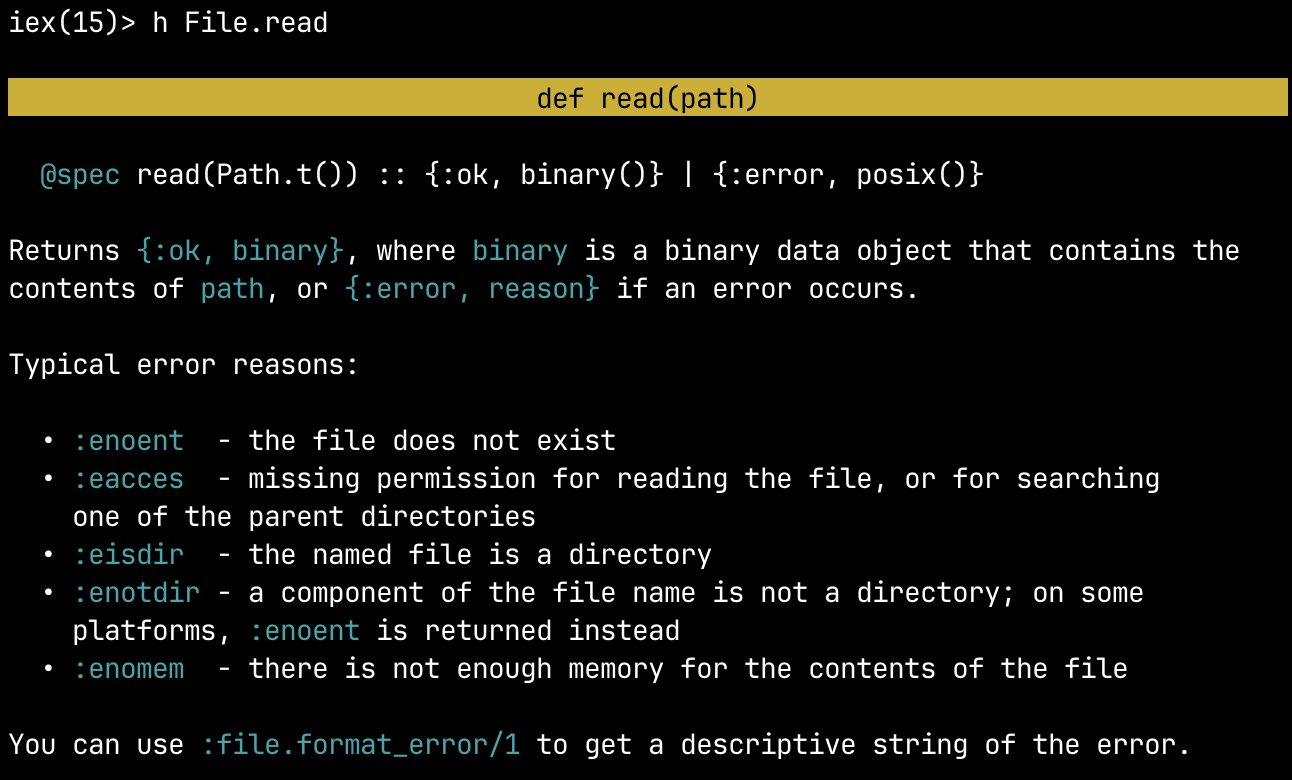
\includegraphics[width=0.8\linewidth]{2_6.png}
    \caption{File.read/1 的文档}
    \label{fig:2_6}
\end{figure}

你会如何编写文件读取部分?更重要的是,从上述文档中我们能学到什么?

\begin{enumerate}
\def\labelenumi{\arabic{enumi}.}

\item
  对于成功的读取,\texttt{File.read/1} 返回一个
  \mintinline{elixir}|{:ok, binary}| 元组。注意
  \texttt{binary} 是读取文件的全部内容。
\item
  否则,将返回 \mintinline{elixir}|{:error, reason}| 元组。变量
  \texttt{reasob}包含错误原因,这是一个原子,如
  \texttt{:enoent} 或
  \texttt{:eacces}。
\end{enumerate}


\begin{code}{}\begin{minted}[linenos]{elixir}
case File.read("KISS - Beth.mp3") do
  {:ok, binary} ->
    IO.puts("KISS rocks!")

  {:error, reason} ->
    IO.puts("No Rock N Roll for anyone today because of #{reason}.")
end
\end{minted}
% \label{lst:reading_a_file}
\end{code}


\begin{example}{井字棋盘}

以下是使用元组的井字棋应用程序的一个示例。在这个例子中,我们有一个\texttt{check\_board/1}函数,它检查井字棋的棋盘配置。棋盘是使用元组表示的。注意我们如何使用元组``绘制''棋盘,以及代码是多么易于理解:

\begin{code}{}% \captionof{listing}{井字棋}
\begin{minted}[linenos]{elixir}
def check_board(board) do
  case board do
    {:x, :x, :x, _, _, _, _, _, _} -> :x_win
    {_, _, _, :x, :x, :x, _, _, _} -> :x_win
    {_, _, _, _, _, _, :x, :x, :x} -> :x_win
    {:x, _, _, :x, _, _, :x, _, _} -> :x_win
    {_, :x, _, _, :x, _, _, :x, _} -> :x_win
    {_, _, :x, _, _, :x, _, _, :x} -> :x_win
    {:x, _, _, _, :x, _, _, _, :x} -> :x_win
    {_, _, :x, _, :x, _, :x, _, _} -> :x_win
    # Player O board patterns omitted ...

    {a, b, c, d, e, f, g, h, i} when a and b and c and d and e and f and g and h and i -> :draw
    _ -> :in_progress
  end
end
\end{minted}
% \label{lst:tictactoe}
\end{code}

`\texttt{\_}' 是 ``不关心'' 或 ``匹配一切''运算符。在本书中你将看到很多这样的例子。在下一节中,我们将看到更多模式匹配的例子,其中我们将讨论\emph{列表}。
\end{example}

\begin{example}{解析MP3文件}
\end{example}

Elixir非常适合解析二进制数据。在这个例子中,我们将从MP3文件中提取元数据。这也是一个很好的练习,以加强你之前学到的一些概念。在解析任何二进制之前,你必须知道文件布局(layout)。我们感兴趣的信息,\emph{ID3标签},位于mp3二进制的\emph{最后128字节}:

\begin{figure}[!ht]
    \centering
    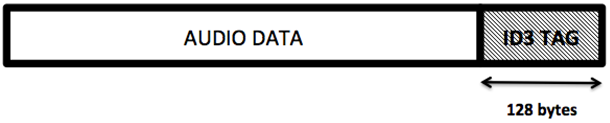
\includegraphics[width=0.8\linewidth]{2_7.png}
    \caption{ID3标签位于MP3二进制的最后128字节。}
    \label{fig:2_7}
\end{figure}

这意味着我们必须以某种方式忽略音频数据部分,只关注ID3标签。下图显示了ID3标签的布局:

\begin{figure}[!ht]
    \centering
    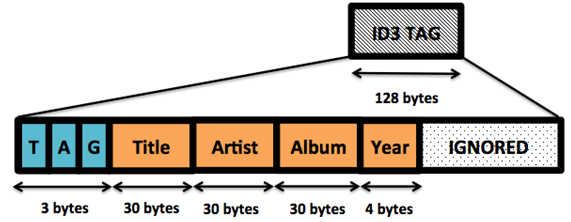
\includegraphics[width=0.8\linewidth]{2_8.png}
    \caption{ID3标签的布局}
    \label{fig:2_8}
\end{figure}

ID3标签的前三个字节称为头部,包含三个字符:``T'',``A''和``G''。接下来的30个字节包含\emph{标题(title)}。然后是30个字节的\emph{艺术家(artist)},接着是另外30个字节的\emph{专辑(album)}。接下来的4个字节是\emph{年份(year)}(例如:``2'',``0'',``1'',``4'')。试想你会如何在其他编程语言中实现这一点。这是Elixir版本的实现,请将此文件保存为\texttt{id3.ex}。

\begin{code}{}
\begin{minted}[linenos]{elixir}
defmodule ID3Parser do
  def parse(file_name) do
    case File.read(file_name) do #1
      {:ok, mp3} -> #2
        mp3_byte_size = byte_size(mp3) – 128 #4
        << _ :: binary-size(mp3_byte_size), id3_tag :: binary >> = mp3 #5 使用模式匹配从MP3二进制数据中捕获ID3标签的字节。
        << "TAG", title   :: binary-size(30),
          artist  :: binary-size(30),
          album   :: binary-size(30),
          year    :: binary-size(4),
          _rest   :: binary >>       = id3_tag #6
        IO.puts "#{artist} - #{title} (#{album}, #{year})"
      _ -> #3
        IO.puts "Couldn't open #{file_name}"
    end
  end
end

#1 读取MP3二进制数据。
#2 成功读取文件返回一个匹配此模式的元组。
#3 文件读取失败则与其他任何内容匹配。
#4 计算MP3音频部分的字节大小。
#5 使用模式匹配从MP3二进制数据中捕获ID3标签的字节。
#6 使用模式匹配从ID3标签中捕获各种ID3字段。
\end{minted}
% \label{lst:id}
\end{code}



程序运行示例:

\begin{code}{}
\begin{minted}[linenos]{elixir}
% iex id3.ex
iex(1)> ID3Parser.parse "sample.mp3"
\end{minted}
% \label{lst:id}
\end{code}

程序运行结果示例:

\begin{code}{}
\begin{minted}[linenos]{elixir}
Lana Del Rey - Ultraviolence (Ultraviolence, 2014)
:ok
\end{minted}
% \label{lst:id}
\end{code}

让我们来回顾一下程序的运行过程。首先,程序读取MP3的二进制数据。正常情况下会返回一个匹配\mintinline{elixir}|{:ok, mp3}|的元组,其中\texttt{mp3}包含文件的二进制内容。否则,通用的\texttt{\_}操作符将匹配文件读取失败的情况。

由于我们只关注ID3标签,因此需要找到一种方法来``跳过''前面的部分。我们首先计算二进制音频部分的\emph{字节大小}。现在我们有了这个信息,就可以告诉Elixir如何解构二进制数据。我们通过在左边声明一个模式,并在右边使用mp3变量来进行模式匹配。请记住,变量赋值在左边,否则尝试进行模式匹配。

\begin{figure}[!ht]
    \centering
    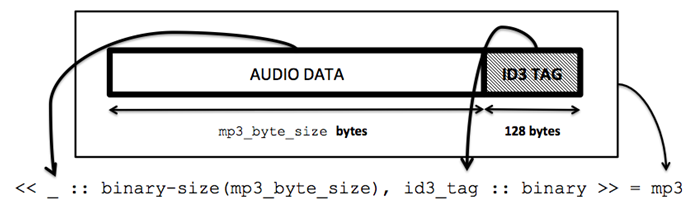
\includegraphics[width=0.8\linewidth]{2_9.png}
    \caption{二进制数据的解构方式}
    \label{fig:2_9}
\end{figure}

你可能认出了\texttt{<< >>}。它用于表示一个二进制数据。然后我们声明我们对音频部分不感兴趣。我们如何做到这一点呢?我们通过指定之前计算出的二进制大小来实现。剩下的就是ID3标签,被捕获到\texttt{id3\_tag}变量中。现在我们可以自由地从ID3标签中提取信息了!

为了做到这一点,我们进行了另一个模式匹配,左边声明了模式,右边是\texttt{id3\_tag}。通过声明适当数量的字节,标题、艺术家和其他信息被捕获到相应的变量中。

\begin{figure}[!ht]
    \centering
    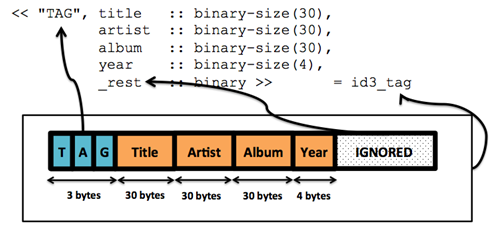
\includegraphics[width=0.8\linewidth]{2_10.png}
    \caption{解构ID3二进制数据}
    \label{fig:2_10}
\end{figure}

\section{列表}

列表是 Elixir
中的另一种数据类型。列表有许多有趣的用途,因此值得单独讨论。列表在某种程度上类似于\emph{链表}\pagenote{http://en.wikipedia.org/wiki/Linked\_list},因为随机访问基本上是一个
O(n) 线性操作。下面是列表的定义:

\begin{quote}
\textbf{一个非空列表由头部和尾部组成。尾部也是一个列表。}
\end{quote}

请注意上述定义的递归性质。转换成代码就是:

\begin{code}{}
\begin{minted}[linenos]{elixir}
iex > [1, 2, 3] == [1 | [2 | [3 | []]]]
true
\end{minted}
% \label{lst:id}
\end{code}

一个图示可能更能说明这一点:

\begin{figure}[!ht]
    \centering
    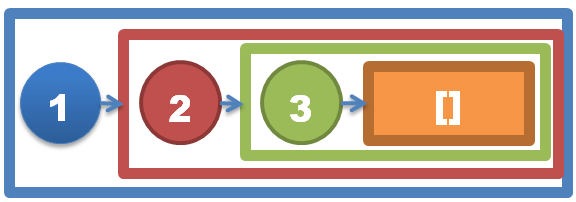
\includegraphics[width=0.8\linewidth]{2_11.png}
    \caption{[1,2,3]的图示表示}
    \label{fig:2_11}
\end{figure}


让我们从最外层的盒子开始理解这幅图。这表明列表的头部是1,随后是列表的尾部。这个尾部,又是另一个列表。这次,这个列表的头部是2,随后是尾部,这个尾部(再次)是另一个列表。

最终,这个列表(从第三个封闭盒子)由一个头部 3和一个尾部组成。这个尾部是一个空列表。实际上,\emph{任何列表的最后一个元素的尾部总是一个空列表}。递归函数利用这一事实来确定列表何时结束。

您还可以使用模式匹配运算符来证明两边确实是同一回事:

\begin{code}{左侧和右侧是等价的}
\begin{minted}[linenos]{elixir}
iex > [1, 2, 3] = [1 | [2 | [3 | []]]]
[1, 2, 3]
\end{minted}
\label{lst:left_and_right_are_equivalent}
\end{code}

由于没有\texttt{MatchError}发生,我们可以确定这两种表示列表的方法是等价的。当然,您不会在日常代码中输入\texttt{[1|[2|[3|[]]]]}。这只是为了强调列表是一种递归数据结构。

我还没有解释`\texttt{|}'是什么。'\texttt{|}'运算符通常被称为\emph{cons}运算符\pagenote{\texttt{construct}的缩写. 参考\url{http://en.wikipedia.org/wiki/Cons}获得更多信息.}。应用于列表时,它用于分隔头部和尾部。也就是说,列表被\emph{解构}了。这是模式匹配的又一个实例。

\begin{code}{使用 cons 运算符解构列表}
\begin{minted}[linenos]{elixir}
iex > [head | tail] = [1, 2, 3]
[1, 2, 3]
\end{minted}
\label{lst:use_the_cons_operator_to_destructure_a_list}
\end{code}

让我们检查 head 和 tail 的内容:

\begin{code}{}
\begin{minted}[linenos]{elixir}
iex > head
1
# A``[2, 3]`
iex > tail
# A 这也是一个列表
\end{minted}
% \label{lst:id}
\end{code}

注意\texttt{tail}也是一个列表,这符合定义。您还可以使用cons 运算符向列表的开头\emph{添加}(或追加):

\begin{code}{使用 cons 运算符向列表中追加}
\begin{minted}[linenos]{elixir}
iex(1) > list = [1, 2, 3]
[1, 2, 3]
iex(2) > [0 | list]
[0, 1, 2, 3]
\end{minted}
\label{lst:use_the_cons_operator_to_append_to_a_list}
\end{code}

我们还可以使用\texttt{++}运算符来连接列表:

\begin{code}{使用 ++ 运算符连接列表}
\begin{minted}[linenos]{elixir}
iex(3) > [0] ++ [1, 2, 3]
[0, 1, 2, 3]
\end{minted}
\label{lst:use_the_++_operator_to_concatenate_lists}
\end{code}

那么单个元素的列表呢?如果您理解了之前的列表图示,那么这将是小菜一碟。

\begin{code}{单元素列表的尾部匹配为空列表}
\begin{minted}[linenos]{elixir}
iex(22) > [head | tail] = [:lonely]
[:lonely]
iex(23) > head
:lonely
iex(24) > tail
[]
\end{minted}
\label{lst:single_element_list_tail_matches_an_empty_list}
\end{code}

这里我们有一个包含单个原子的列表。现在注意我们的\texttt{tail}是一个空列表。起初这可能看起来有些奇怪,但如果您仔细思考,它符合定义。正是这种定义使我们能够用列表和递归做一些有趣的事情,我们接下来会进行探索。


\begin{example}{展平列表}
\end{example}

现在您了解了列表的工作原理,让我们来构建我们自己的\texttt{flatten/1}。\texttt{flatten/1}接受一个可能嵌套的列表,并返回一个展平的版本。展平列表特别有用,尤其是当列表用于表示树\pagenote{http://en.wikipedia.org/wiki/Tree\_\%28data\_structure\%29\#Representations}数据结构时。因此,展平树会返回树中包含的所有元素。让我们看一个例子:

\begin{code}{}
\begin{minted}[linenos]{elixir}
List.flatten([1, [:two], ["three", []]])
\end{minted}
% \label{lst:id}
\end{code}

将返回\texttt{[1, :two, "three"]}。这是\texttt{flatten/1} 的一种可能实现:

\begin{code}{展平列表的可能实现}
\begin{minted}[linenos]{elixir}
defmodule MyList do
  def flatten([]), do: [] #1
  def flatten([ head | tail ]) do  #2
    flatten(head) ++ flatten(tail) #2
  end
  def flatten(head), do: [ head ]  end #3

#1 基本情况,一个空列表
#2 非空列表,有多于 1 个元素
#3 单元素列表
\end{minted}
\label{lst:possible_implementation_of_flattening_a_list}
\end{code}


花点时间消化这段代码,因为它不仅仅是表面看起来那样。需要考虑3种情况:

我们从基本情况(或者如果您上过一些计算机科学课程的话,退化情况)开始------ 空列表:

1. 如果我们得到一个空列表,我们只需返回一个空列表。 

2. 对于非空列表,我们使用 cons运算符将其分解为\texttt{head}和\texttt{tail}。然后我们递归地调用\texttt{flatten/1}处理\texttt{head}和\texttt{tail}。接下来,使用\texttt{++}运算符将结果连接起来。注意\texttt{head}也可能是一个嵌套列表。例如,\texttt{[[1], 2]}意味着\texttt{head}是\texttt{[1]}。

如果我们得到一个非列表参数,我们将其转换成一个列表。现在,考虑(最好在纸上跟踪)对像\texttt{[[1], 2]}
这样的列表的处理。让我们跟踪执行过程:

1. 第一个函数子句 \#1 不匹配。 

2. 第二个函数子句 \#2匹配。在这种情况下,我们对列表进行模式匹配,\texttt{head}是\texttt{[1]},而\texttt{tail}是\texttt{2}。现在,\texttt{flatten([1])}和\texttt{flatten(2)}被递归调用。

3. 处理\texttt{flatten([1])}。它同样不匹配第一个子句\#1。第二个子句 \#2匹配。~\texttt{head}~是\texttt{1},而\texttt{tail}是\texttt{[]}。

4. 现在调用\texttt{flatten(1)},第三个函数子句 \#3匹配,返回\texttt{[1]}。\texttt{flatten[])}匹配第一个子句,返回\texttt{[]}。之前对\texttt{flatten(2)}的调用(见第2步)返回\texttt{[2]}。\texttt{[1] ++ [] ++ [2]}生成了我们的展平列表。

不要灰心,如果你第一次没有完全理解。就像大多数事情一样,多一些练习会有很大的帮助。此外,在接下来的章节中,你将看到许多例子。

\subsection{函数子句(Function Clauses)的排序}

我之前提到过,函数子句(Function Clauses)的\emph{顺序}很重要。这是一个完美的例子来解释为什么:

\begin{code}{函数子句(Function Clauses)的顺序很重要}
\begin{minted}[linenos]{elixir}
defmodule MyList do
  def flatten([head | tail]) do
    flatten(head) ++ flatten(tail)
  end

  def flatten(head), do: [head]

  # 1 这行永远不会运行!
  def flatten([]), do: []
end
\end{minted}
\label{lst:the_order_of_function_clauses_is_important}
\end{code}

我们将基本情况设为了最后一个子句。想一想,当我们尝试\texttt{MyList.flatten([])}时会发生什么?我们期望得到\texttt{[]},但实际上我们得到了\texttt{[[]]}。如果你仔细思考一下,你会意识到\#1从未被执行。原因是第二个函数子句会匹配\texttt{[]},因此第三个函数子句将被忽略。

让我们真正运行一下这个程序:


\begin{code}{Elixir 会有帮助地警告未匹配的子句}
\begin{minted}[linenos]{elixir}
% iex length_converter.ex
warning: this clause cannot match because a previous clause at line 7 always matches
\end{minted}
\label{lst:elixir_will_helpfully_warn_about_unmatched_clauses}
\end{code}

Elixir在背后默默支持我们!像这样的警告值得注意,因为它们可以节省你数小时的调试头痛。而未匹配的条款可能意味着无效代码,或者在更糟糕的情况下,是一个无限循环。

\section{管道运算符\texttt{|>}}

现在,我想介绍编程语言史上最有用的运算符之一 -\texttt{|>} \pagenote{\texttt{|>} 操作符收到了F\#的启发.}。
这个运算符将左边表达式的结果作为右边函数调用的第一个参数。这是我最近写的一个Elixir程序中的代码片段。如果没有管道运算符,我会这样写它:

\begin{code}{没有 \texttt{|>}运算符(或者,大多数语言的做法)}
\begin{minted}[linenos]{elixir}
defmodule URLWorker do
  def start(url) do
    do_request(HTTPoison.get(url))
  end

  # ...
end
\end{minted}
\label{lst:without_the_pipe_operator_or_the_way_most_languages_do_it}
\end{code}

\texttt{HTTPoison} 是一个 HTTP 客户端。它接收一个\texttt{url} 并返回 HTML 页面。然后将页面传递给\texttt{do\_request}函数进行一些解析。注意,在这个版本中,你必须寻找最内层的括号来定位\texttt{url},然后在你脑子里追踪连续的函数调用向外移动。

我向你展示带有管道运算符的版本:

\begin{code}{使用 \texttt{|>} 运算符}
\begin{minted}[linenos]{elixir}
defmodule URLWorker do
  def start(url) do
    result = url |> HTTPoison.get() |> do_request
  end

  # ...
end
\end{minted}
\label{lst:use_pipe_operator}
\end{code}

很清晰对吧?许多例子将广泛使用 \texttt{|>}。你越多使用\texttt{|>},就越会开始看到\emph{数据正在从一种形式转换}到另一种,就像装配线一样。事实上,一旦你经常使用它,当你在其他语言中编程时,你会开始想念它。


\begin{example}{按文件名过滤目录中的文件}
\end{example}

假设我有一个装满电子书的目录,这个目录可能嵌套有文件夹。我想只获取 EPUB的文件名。例如,我只想要文件名以 \texttt{*.epub}
结尾且包含 ``Java'' 的书籍。这是我的做法:

\begin{code}{过滤包含 ``Java'' 的 epub}
\begin{minted}[linenos]{elixir}
# 1
"/Users/Ben/Books"
# 2
|> Path.join("**/*.epub")
# 3
|> Path.wildcard()
# 4
|> Enum.filter(fn fname ->
  String.contains?(Path.basename(fname), "Java")
end)
\end{minted}
\label{lst:filter_epubs_containing_java}
\end{code}

\#1 是目录的字符串表示。在 \#2中,我们构造了一个带通配符的路径。此外,我们指定我们只对 EPUB感兴趣。这个结果传递给\#3。通配符函数读取路径,并返回匹配的文件名列表。这反过来又传递到 \#4中的过滤函数,只选择包含 ``Java''的文件名。阅读如此明确和显而易见地描述其步骤的代码是非常好的。

一个示例输出看起来像:
\begin{minted}[linenos]{bash}
["/Users/Ben/Books/Java/Java_Concurrency_In_Practice.epub",
 "/Users/Ben/Books/Javascript/JavaScript Patterns.epub",
 "/Users/Ben/Books/Javascript/Functional_JavaScript.epub",
 "/Users/Ben/Books/Ruby/Using_JRuby_Bringing_Ruby_to_Java.epub"]
\end{minted}

 \section{Erlang与Elixir互操作性}

由于Elixir和Erlang共享相同的字节码,因此在性能方面调用Erlang代码不会有任何影响。更重要的是,这意味着您可以自由地使用任何Erlang库与您的Elixir代码一起使用。

\subsection{从Elixir调用Erlang函数}

唯一的注意点是\emph{如何}调用代码。例如,您可以像这样在Erlang中生成一个随机数:

\begin{code}{在Erlang中生成随机数}
\begin{minted}[linenos]{erlang}
1> random:uniform(123)
55
\end{minted}
\label{lst:generate_a_random_number_in_erlang}
\end{code}

这个函数是Erlang标准发行版的一部分。我可以在Elixir中用一些语法调整调用相同的Erlang函数:


\begin{code}{将 \texttt{random:uniform().}翻译为Elixir}
\begin{minted}[linenos]{elixir}
iex > :random.uniform(123)
55
\end{minted}
\label{lst:use_the_random_uniform_function_in_elixir}
\end{code}

注意两个代码中冒号和点的位置。这就是全部!在Elixir中使用原生Erlang函数时有一个小注意点。您无法从\texttt{iex}访问Erlang函数的文档:

\begin{code}{在iex中无法获得Erlang文档}
\begin{minted}[linenos]{elixir}
iex(3)> h :random
:random 是一个Erlang模块,因此它没有Elixir风格的文档
\end{minted}
\label{lst:cannot_get_erlang_docs_in_iex}
\end{code}

调用Erlang函数在Elixir中没有相应实现的标准库时非常有用。如果您比较Erlang和Elixir的标准库,可能会得出Erlang的库功能更加丰富的结论。但如果您仔细想想,Elixir实际上免费获得了一切!


\subsubsection{在Elixir中调用Erlang的HTTP客户端}

通常,如果我发现Elixir缺少我想要的某个功能,我会首先检查是否有Erlang标准库函数可以使用,然后才搜索第三方库。例如,我曾想在Elixir中构建一个网络爬虫。构建网络爬虫的第一步之一就是能够下载网页。这需要一个HTTP客户端。Elixir没有内置的HTTP客户端------它不需要,因为Erlang有一个,恰当地命名为\texttt{httpc}\pagenote{http://erlang.org/doc/man/httpc.html\#request-1}。

假设我想下载某个编程语言的网页。我查阅了Erlang文档\pagenote{骗你的,在现实中我可能会首先访问StackOverflow},找到了我需要的内容:

\begin{figure}[!ht]
    \centering
    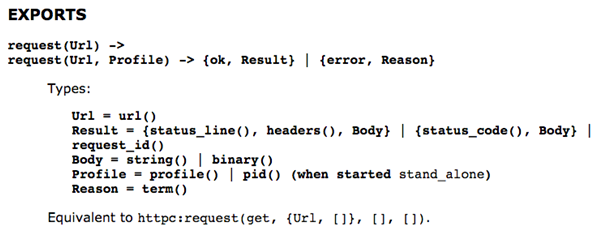
\includegraphics[width=0.8\linewidth]{2_6a.png}
    \caption{Erlang文档中的httpc:request/1}
    \label{fig:2_6a}
\end{figure}

首先,我需要启动\texttt{inets}应用程序(文档中有说明),然后进行实际的请求:


\begin{code}{使用Erlang的httpc库下载网页}
\begin{minted}[linenos]{elixir}
iex(1)> :inets.start
:ok
iex(2)> {:ok, {status, headers, body}} = :httpc.request 'http://www.elixir-lang.org'
{:ok,
 {{'HTTP/1.1', 200, 'OK'},
  [{'cache-control', 'max-age=600'}, {'date', 'Tue, 28 Oct 2014 16:17:24 GMT'},
   {'accept-ranges', 'bytes'}, {'server', 'GitHub.com'},
   {'vary', 'Accept-Encoding'}, {'content-length', '17251'},
   {'content-type', 'text/html; charset=utf-8'},
   {'expires', 'Tue, 28 Oct 2014 16:27:24 GMT'},
   {'last-modified', 'Tue, 21 Oct 2014 23:38:22 GMT'}],
  [60, 33, 68, 79, 67, 84, 89, 80, 69, 32, 104, 116, 109, 108, 62, 10, 60, 104,
   116, 109

, 108, 32, 120, 109, 108, 110, 115, 61, 34, 104, 116, 116, 112, 58, 47, 47, 119, 119, 119, 46, 119, 51, 46, 111, 114, 103, 47, 49, 57, 57, ...]}}
\end{minted}
\label{lst:downloading_a_web_page_with_erlangs_httpc_library}
\end{code}


\subsubsection{还有一件事\ldots\ldots{}}

Erlang还有一个非常整洁的GUI前端,名为\emph{Observer},让您能够检查Erlang虚拟机等内容。调用它很简单:

\begin{code}{调用Observer,一个内置的Erlang工具}
\begin{minted}[linenos]{elixir}
iex(1) > :observer.start()
\end{minted}
\label{lst:use_erlang_observer}
\end{code}

由于您当前没有运行任何计算密集型进程,因此现在不会看到太多动作。图\ref{fig:2_7a}供您预览:

\begin{figure}[!ht]
    \centering
    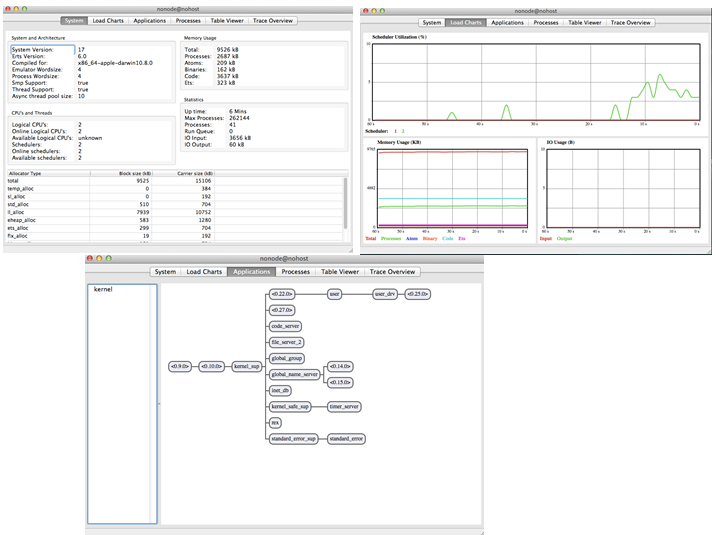
\includegraphics[width=0.8\linewidth]{2_7a.png}
    \caption{Observer的截图}
    \label{fig:2_7a}
\end{figure}

Observer在查看VM承受的负载、监督树的布局(您将在后面的章节学习到这一点)以及查看Erlang提供的内置数据库中存储的数据方面非常有用。

 \section{练习}

这是一个相当长的章节。现在是时候确保你理解了章节中的所有内容。

\begin{enumerate}
\def\labelenumi{\arabic{enumi}.}

\item 实现 \texttt{sum/1}函数。这个函数应该接收一个数字列表,并返回该列表的总和。
\item 探索 \texttt{Enum} 模块。
\item 将 \texttt{[1,[[2],3]]} 转换为\texttt{[9, 4, 1]},分别使用和不使用管道操作符。
\item 将 Erlang 中的\texttt{crypto:md5("Tales from the Crypt").} 翻译为
  Elixir。
\item 探索官方的 Elixir入门指南
	  \pagenote{http://elixir-lang.org/getting\_started/1.html}。
\item
  看看一个 IPV4 数据包。尝试编写一个解析器。
\end{enumerate}

\section{总结}

这结束了我们的快速旅程。如果你坚持到了这里,请给自己一个赞。如果你还没有理解所有内容,不用担心。许多概念会在途中变得清晰,一旦你看到它们的应用,许多编程结构会变得显而易见。作为一个快速回顾,这里是我们刚刚学到的内容:

\begin{itemize}

\item  Elixir 的基本数据类型。
\item  守护子句(Guards),以及它们如何与函数子句很好地协作。
\item  模式匹配,以及它如何导致非常声明式的代码。我们还看了一些模式匹配的实际例子。
\item  列表,另一个基本的数据结构。我们还看到了列表在 Elixir  中如何内部表示,以及这如何促进递归。
\item  Elixir 和 Erlang 如何良好地协同工作。
\end{itemize}

在下一章中,我们将学习 Elixir 中并发的基本单位------进程。这是 Elixir与传统编程语言截然不同的特性之一。

\printnotes*
\chapter{进程101}\label{chapt:processes}

本章内容包括:

\begin{itemize}

\item  Actor并发模型(Actor Concurrency Model)
\item  创建进程
\item  如何使用进程发送和接收消息
\item  使用进程实现并发
\item  如何使进程相互通信
\end{itemize}

理解进程的概念是非常重要的,它理所当然地拥有自己的一章。进程是Elixir中并发的基本单位。实际上,Erlang虚拟机(Erlang VM)支持高达1.34亿个进程,这使得所有的CPU都能愉快地运转。知道我充分利用了硬件资源,总是让我有一种温暖、愉悦的感觉。Erlang虚拟机创建的进程与操作系统无关。这些进程更轻量级,创建它们仅需要几微秒。

我们将开始一个有趣的项目。在本章中,我们将构建一个简单的程序,用于报告特定城市/州/国家的温度。但首先,让我们了解一下actor并发模型。

\section{Actor并发模型}

Erlang(因此也包括Elixir)使用Actor并发模型。这意味着:

\begin{itemize}
	\item 每个\emph{actor}都是一个\emph{进程}。 
  \item 每个进程执行一个\emph{特定任务}。 
  \item 要让进程做某事,你需要\emph{向它发送消息}。进程也可以通过\emph{发送回另一个消息}来回复。
  \item 进程可以处理的消息类型特定于进程本身。换句话说,消息是\emph{模式匹配}的。
  \item 除此之外,进程\emph{不与其他进程共享任何信息}。
\end{itemize}

如果这一切现在看起来还有些模糊,不要担心。如果你做过面向对象编程,你会发现进程在很多方面类似于对象。甚至可以说它是更纯粹的面向对象形式。

这里有一个思考actors的方式。Actors就像人一样。我们通过相互交谈来交流。例如,我的妻子告诉我洗碗。当然,我会通过洗碗来回应——我是个好丈夫。但如果我的妻子告诉我吃蔬菜,她会被忽略——我不会对此作出回应。实际上,我选择只对某些类型的消息做出回应。最后,我不知道她脑海中在想什么,她也不知道我脑海中在想什么。正如你将很快看到的,actor并发模型就像这样——只对某些类型的消息做出回应。

\section{构建天气应用}

从概念上讲,我们的应用程序非常简单。第一个版本接受一个包含位置的单个参数,并报告摄氏温度。这涉及向外部天气服务发出HTTP请求,并解析JSON响应以提取温度。

\begin{figure}[!ht]
    \centering
    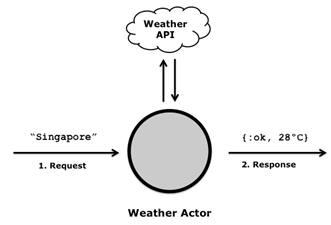
\includegraphics[width=0.8\linewidth]{3_1.png}
    \caption{天气actor处理单个请求}
    \label{fig:3_1}
\end{figure}


进行单个请求是微不足道的。但如果我们想要同时了解100个城市的温度怎么办?假设每个请求需要1秒钟,我们要等待100秒吗?显然不是!我们将看到如何进行并发请求,以便尽快获得结果。

并发的一个特性是,我们永远不知道响应以何种顺序返回。例如,想象一下,我按字母顺序传入一个城市列表。我收到的回应绝对不保证以相同的顺序排列。

我们如何确保响应的顺序是正确的呢?亲爱的读者,继续阅读下去,因为我们现在就开始在Elixir中的气象冒险。

 \subsection{简单版本}

我们从一个简单版本开始。也就是说,不会涉及到并发。另一方面,简单版本将包含所有需要发出请求、解析响应和返回结果的逻辑。在本章的结束时,你将学习如何:

\begin{itemize}

\item  使用mix安装和使用第三方库
\item  向第三方API发出HTTP请求
\item  使用模式匹配解析JSON响应
\item  看看管道如何促进数据转换
\end{itemize}

这将是你要处理的第一个non-trival的程序。但是不用担心,你将在每一步都得到指导。让我们开始吧!

\subsubsection{创建一个新项目}

首要任务是创建一个新项目,更重要的是,给它起一个好名字。既然我是作者,我就来选择名字。在代码\ref{lst:create_new_project}中,我们使用\texttt{mix new <project name>} 来创建一个新项目


\begin{code}{创建一个新项目}
\begin{minted}[linenos]{bash}
% mix new metex
* creating README.md
* creating .gitignore
* creating mix.exs
* creating config
* creating config/config.exs
* creating lib
* creating lib/metex.ex
* creating test
* creating test/test_helper.exs
* creating test/metex_test.exs
Your mix project was created successfully.
You can use mix to compile it, test it, and more:

cd metex
mix test
% cd metex
\end{minted}
\label{lst:create_new_project}
\end{code}

按照指示,进入\texttt{metex}目录。

\subsubsection{安装依赖项}

打开\texttt{mix.exs}。你会看到以下内容:

\begin{code}{ 默认生成的mix.exs文件}
\begin{minted}[linenos]{elixir}
defmodule Metex.Mixfile do
  use Mix.Project

  def project do
    [app: :metex, version: "0.0.1", elixir: "~> 1.0", deps: deps]
  end

  def application do
    [applications: [:logger]]
  end

  defp deps do
    []
  end
end
\end{minted}
\label{lst:defautl_mix_exs}
\end{code}

每个由\texttt{mix}生成的项目都会包含这个文件。它由两个公共函数组成,\texttt{project}和\texttt{application}。这个\texttt{project}函数基本上是设置我们的项目。更重要的是,它通过调用\texttt{deps}私有函数来设置我们项目的依赖项。就目前而言,\texttt{deps}是一个空列表-暂时的。这个\texttt{application}函数用于生成一个应用资源文件。Elixir中的某些依赖项需要以特定的方式启动。像这样的依赖项在此函数中声明。例如,在我们的应用程序启动之前,先启动\texttt{logger}应用程序。

让我们通过修改\texttt{deps}函数来添加两个依赖项,像代码\ref{lst:deps_in_mix_exs}这样:

\textbf{代码3.3 }

\begin{code}{在mix.exs中声明依赖项}
\begin{minted}[linenos]{elixir}
defp deps do
    [
    {:httpoison, "~> 0.9.0"},  #1
    {:json,      "~> 0.3.0"}   #1
    ]
end

#1 声明依赖项并指定相应的版本号
\end{minted}
\label{lst:deps_in_mix_exs}
\end{code}

\

接下来,在\texttt{application}函数中添加一个条目:

\begin{code}{}
\begin{minted}[linenos]{elixir}
def application do
  [applications: [:logger, :httpoison]]
end
\end{minted}
% \label{lst:id}
\end{code}

我怎么知道我应该包括\texttt{:httpoison},而不是说,\texttt{:json}?事实上,我不知道。所以我总是做下一个最好的事情-阅读详细的手册。每次我安装一个库,我首先看一下README。在\texttt{:httpoison}的情况下,README清楚地说明了:

\begin{figure}[!ht]
    \centering
    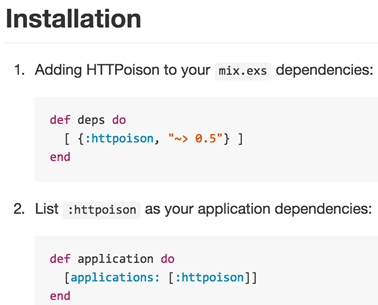
\includegraphics[width=0.8\linewidth]{3_2.png}
    \caption{查看第三方库的README以获取重要的安装指令}
    \label{fig:3_2}
\end{figure}

\subsubsection{依赖项版本号很重要!}

注意你的依赖项的版本号。使用错误的版本号可能会导致令人困惑的错误。另一件需要注意的事情是,这些库中的许多都会指定它们与之兼容的Elixir的最小版本。

确保你在Metex目录中,我们可以使用\texttt{mix deps.get}命令来安装我们的依赖项:

\texttt{\% mix deps.get}
注意到\texttt{mix}也有助于解决依赖项。在这种情况下,它引入了另外两个库,\texttt{hackney}和\texttt{idna}(代码\ref{lst:deps_get}):

\begin{code}{mix 自动解决依赖关系}
\begin{minted}[linenos]{elixir}
% mix deps.get
Running dependency resolution
* Getting httpoison (Hex package)
Checking package (http://s3.hex.pm.global.prod.fastly.net/tarballs/httpoison-0.9.0.tar)
Using locally cached package
* Getting json (Hex package)
Checking package (http://s3.hex.pm.global.prod.fastly.net/tarballs/json-0.3.2.tar)
Using locally cached package
* Getting hackney (Hex package)
Checking package (http://s3.hex.pm.global.prod.fastly.net/tarballs/hackney-1.5.7.tar)
Using locally cached package
* Getting ssl_verify_fun (Hex package)
Checking package (http://s3.hex.pm.global.prod.fastly.net/tarballs/ssl_verify_fun-1.1.0.tar)
Using locally cached package
* Getting mimerl (Hex package)
Checking package (http://s3.hex.pm.global.prod.fastly.net/tarballs/mimerl-1.0.2.tar)
Using locally cached package
* Getting metrics (Hex package)
Checking package (http://s3.hex.pm.global.prod.fastly.net/tarballs/metrics-1.0.1.tar)
Using locally cached package
* Getting idna (Hex package)
Checking package (http://s3.hex.pm.global.prod.fastly.net/tarballs/idna-1.2.0.tar)
Using locally cached package
* Getting certifi (Hex package)
Checking package (http://s3.hex.pm.global.prod.fastly.net/tarballs/certifi-0.4.0.tar)
Using locally cached package
\end{minted}
\label{lst:deps_get}
\end{code}

\section{Worker模块}

在我们开始实现Worker模块之前,我们需要从第三方天气服务OpenWeatherMap获取一个API密钥。请访问\texttt{http://openweathermap.org/}创建一个账户。完成后,你会看到你的API密钥已经为你创建好了:

\begin{figure}[!ht]
    \centering
    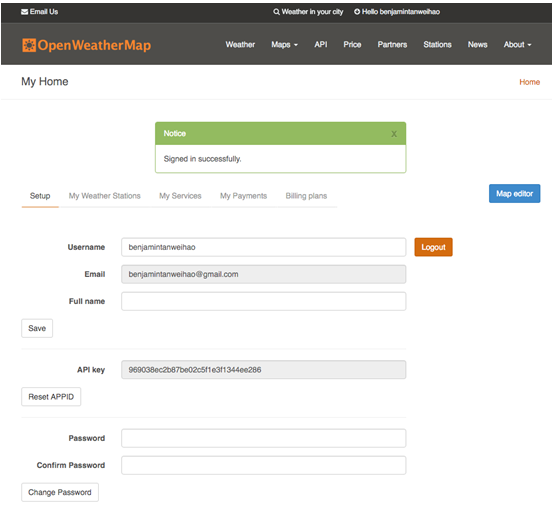
\includegraphics[width=0.8\linewidth]{3_3.png}
    \caption{在OpenWeatherMap创建账户并获取API密钥}
    \label{fig:3_3}
\end{figure}


现在我们可以深入了解Worker模块的实现细节。Worker模块的工作是从OpenWeatherMap获取给定位置的温度,并解析结果。在\texttt{lib} 目录中创建
\texttt{worker.ex}。以下是Worker模块的完整列表(代码\ref{lst:worker_ex_code}):


\begin{code}{worker.ex的完整源码。保存在lib/worker.ex中}
\begin{minted}[linenos]{elixir}
defmodule Metex.Worker do
  def temperature_of(location) do
    result = url_for(location) |> HTTPoison.get() |> parse_response

    case result do
      {:ok, temp} ->
        "#{location}: #{temp}°C"

      :error ->
        "#{location} not found"
    end
  end

  defp url_for(location) do
    location = URI.encode(location)
    "http://api.openweathermap.org/data/2.5/weather?q=#{location}&appid=#{apikey}"
  end

  defp parse_response({:ok, %HTTPoison.Response{body: body, status_code: 200}}) do
    body |> JSON.decode!() |> compute_temperature
  end

  defp parse_response(_) do
    :error
  end

  defp compute_temperature(json) do
    try do
      temp = (json["main"]["temp"] - 273.15) |> Float.round(1)
      {:ok, temp}
    rescue
      _ -> :error
    end
  end

  defp apikey do
    "APIKEY-GOES-HERE"
  end
end
\end{minted}
\label{lst:worker_ex_code}
\end{code}

如果你不完全理解正在发生的事情,不要惊慌。我们将一点一点地浏览程序。现在,让我们看看如何从\texttt{iex}运行这个程序。从项目根目录启动\texttt{iex},如下所示:\mintinline{elixir}|% iex –S mix|

如果这是你第一次运行该命令,你会注意到一系列依赖项正在被编译。下次你运行\texttt{iex}时,除非你修改了依赖项,否则你不会看到这个。现在,让我们找出世界上一些最冷的地方的温度(代码\ref{lst:metex_worker_example_run}):

\begin{code}{Metex.Worker的示例运行}
\begin{minted}[linenos]{elixir}
iex(1) > Metex.Worker.temperature_of("Verkhoyansk, Russia")
"Verkhoyansk, Russia: -37.3°C"
\end{minted}
\label{lst:metex_worker_example_run}
\end{code}

只是为了好玩,让我们再试一个:

\begin{code}{}
\begin{minted}[linenos]{elixir}
iex(2) > Metex.Worker.temperature_of("Snag, Yukon, Canada")
"Snag, Yukon, Canada: -27.6°C"
\end{minted}
% \label{lst:id}
\end{code}

当我们给出一个无意义的位置时会发生什么?

\begin{code}{}
\begin{minted}[linenos]{elixir}
iex(3) > Metex.Worker.temperature_of("Omicron Persei 8")
"Omicron Persei 8 not found"
\end{minted}
% \label{lst:id}
\end{code}

现在我们已经看到了Worker模块的行动,让我们仔细看看并弄清楚它是如何工作的。我们从代码\ref{lst:temperature_of}中的\texttt{temperature\_of/1}函数开始:

\begin{code}{Metex.Worker的核心 -\texttt{temperature\_of/1}函数}
\begin{minted}[linenos]{elixir}
defmodule Metex.Worker do

def temperature_of(location) do
    result = url_for(location) |> HTTPoison.get |>  parse_response #1
    case result do
        {:ok, temp} ->                          #2
        "#{location}: #{temp}°C"              #2
        :error ->                               #3
        "#{location} not found"               #3
    end
end

# ...end

#1 数据转换:从URL到HTTP响应,再到解析该响应
#2 成功解析的响应返回温度和位置
#3 否则,返回一个错误消息
\end{minted}
\label{lst:temperature_of}
\end{code}

整个函数中最重要的一行是
\begin{minted}[linenos]{elixir}
result = location \|> url_for \|> HTTPoison.get \|> parse_response
\end{minted}

如果不使用管道操作符,我们将不得不这样编写我们的函数:\mintinline{elixir}|result = parse_response(HTTPoison.get(url_for(location)))|

\texttt{location |> url\_for}构造了用于调用天气API的URL。例如,新加坡的URL将是(用你自己的替换\texttt{<APIKEY>}):
\texttt{http://api.openweathermap.org/data/2.5/weather?q=Singapore\&appid=<APIKEY>}

一旦我们有了URL,我们就可以使用httpoison,一个HTTP客户端,来发出GET请求:
\begin{minted}[linenos]{elixir}
location \|> url_for \|> HTTPoison.get
\end{minted}

如果你在浏览器中尝试了那个URL,你会得到这样的东西(我已经为了简洁而修剪了JSON):

\begin{code}{}
\begin{minted}[linenos]{elixir}
{
...
"main": {
"temp": 299.86,
"temp_min": 299.86,
"temp_max": 299.86,
"pressure": 1028.96,
"sea_level": 1029.64,
"grnd_level": 1028.96,
"humidity": 100
},
...}
\end{minted}
% \label{lst:id}
\end{code}

让我们仔细看看HTTP客户端的响应。也可以在\texttt{iex}中试试这个。如果你退出了\texttt{iex},记得使用\texttt{iex -S mix}
这样依赖项(如httpoison)就能正确加载。

我们可以试试新加坡的温度URL(代码\ref{lst:use_httpoison_get}):

\begin{code}{使用HTTPoison发出GET请求}
\begin{minted}[linenos]{elixir}
iex(1) >
  HTTPoison.get("http://api.openweathermap.org/data/2.5/weather?q=Singapore&appid=<APIKEY>")
\end{minted}
\label{lst:use_httpoison_get}
\end{code}

看看结果:

\begin{code}{}
\begin{minted}[linenos]{elixir}
{:ok,
 %HTTPoison.Response{
   body:
     "{\"coord\":{\"lon\":103.85,\"lat\":1.29},\"sys\":{\"message\":0.098,\"country\":\"SG\",\"sunrise\":1421795647,\"sunset\":1421839059},\"weather\":[{\"id\":802,\"main\":\"Clouds\",\"description\":\"scattered clouds\",\"icon\":\"03n\"}],\"base\":\"cmc stations\",\"main\":{\"temp\":299.86,\"temp_min\":299.86,\"temp_max\":299.86,\"pressure\":1028.96,\"sea_level\":1029.64,\"grnd_level\":1028.96,\"humidity\":100},\"wind\":{\"speed\":6.6,\"deg\":29.0007},\"clouds\":{\"all\":36},\"dt\":1421852665,\"id\":1880252,\"name\":\"Singapore\",\"cod\":200}\n",
   headers: %{
     "Access-Control-Allow-Credentials" => "true",
     "Access-Control-Allow-Methods" => "GET, POST",
     "Access-Control-Allow-Origin" => "*",
     "Connection" => "keep-alive",
     "Content-Type" => "application/json; charset=utf-8",
     "Date" => "Wed, 21 Jan 2015 15:59:14 GMT",
     "Server" => "nginx",
     "Transfer-Encoding" => "chunked",
     "X-Source" => "redis"
   },
   status_code: 200
 }}
\end{minted}
% \label{lst:id}
\end{code}

如果传入一个不存在的页面的URL会怎样?

\begin{code}{}
\begin{minted}[linenos]{elixir}
iex(2) > HTTPoison.get("http://en.wikipedia.org/phpisawesome")
\end{minted}
% \label{lst:id}
\end{code}

这将返回类似这样的东西:

\begin{code}{}
\begin{minted}[linenos]{elixir}
{:ok,
 %HTTPoison.Response{
   body: "<html>Opps</html>",
   headers: %{
     "Accept-Ranges" => "bytes",
     "Age" => "12",
     "Cache-Control" => "s-maxage=2678400, max-age=2678400",
     "Connection" => "keep-alive",
     "Content-Length" => "2830",
     "Content-Type" => "text/html; charset=utf-8",
     "Date" => "Wed, 21 Jan 2015 16:04:48 GMT",
     "Refresh" => "5; url=http://en.wikipedia.org/wiki/phpisawesome",
     "Server" => "Apache",
     "Set-Cookie" => "GeoIP=SG:Singapore:1.2931:103.8558:v4; Path=/; Domain=.wikipedia.org",
     "Via" => "1.1 varnish, 1.1 varnish, 1.1 varnish",
     "X-Cache" => "cp1053 miss (0), cp4016 hit (1), cp4018 frontend miss (0)",
     "X-Powered-By" => "HHVM/3.3.1",
     "X-Varnish" => "2581642697, 646845726 646839971, 2421023671",
     "X-Wikimedia-Debug" => "prot=http:// serv=en.wikipedia.org loc=/phpisawesome"
   },
   status_code: 404
 }}
\end{minted}
% \label{lst:id}
\end{code}

最后,一个荒谬的URL会产生什么呢?

\begin{code}{使用HTTPoison发出无效的GET请求}
\begin{minted}[linenos]{elixir}
iex(3) > HTTPoison.get("phpisawesome")
{:error, %HTTPoison.Error{id: nil, reason: :nxdomain}}
\end{minted}
\label{lst:use_httpoison_get_invalid}
\end{code}

我们刚刚看到了HTTPoison.get(url)可以返回的至少三种变体。正确路径返回一个类似于
\mintinline{elixir}|{:ok, \%HTTPoison.Response\{status_code: 200, body: content\}\}}|
的模式。上面的模式传达了以下信息:

\begin{itemize}

\item  这是一个两元素元组
\item  元组的第一个元素是一个\texttt{:ok}原子,后面跟着一个表示响应的结构
\item  响应是\texttt{HTTPoison.Response}类型的,包含至少两个字段
\item  \texttt{status\_code}的值是200,表示一个成功的\texttt{HTTP  GET}请求
\item  body的值在content中被\emph{捕获}
\end{itemize}

如你所见,模式匹配非常简洁,是表达你想要的东西的一种美丽的方式。同样,错误元组有以下模式:
\mintinline{elixir}|{:error, \%HTTPoison.Error\{reason: reason\}}|。

让我们再做一次相同的分析:
\begin{itemize}

\item  这是一个两元素元组
\item  元组的第一个元素是一个\texttt{:error}原子,后面跟着一个表示错误的结构
\item  响应是\texttt{HTTPoison.Error}类型的,包含至少一个字段,即reason
\item  错误的原因在\texttt{reason}中被捕获
\end{itemize}

牢记这些,让我们看一下\texttt{parse\_response/1}函数(代码\ref{lst:parse_response}):

\begin{code}{parse\_response/1函数中的模式匹配}
\begin{minted}[linenos]{elixir}
defp parse_response({:ok, %HTTPoison.Response{body: body, status_code: 200}}) do
  body |> JSON.decode!() |> compute_temperature
end

defp parse_response(_) do
  :error
end
\end{minted}
\label{lst:parse_response}
\end{code}

在这里,我们指定了\texttt{parse\_response/1}的两个版本。第一个版本匹配成功的GET请求,因为我们正在匹配一个类型为\texttt{HTTPoison.Response}的响应,并确保\texttt{status\_code}是200。否则,我们将任何其他类型的响应视为错误。现在让我们仔细看看\texttt{parse\_response/1}的第一个版本。

\begin{code}{}
\begin{minted}[linenos]{elixir}
defp parse_response({:ok, %HTTPoison.Response{body: body, status_code: 200}}) do
  # ...
end
\end{minted}
% \label{lst:id}
\end{code}

在成功的模式匹配后,JSON的字符串表示被捕获在body变量中。为了将其转换为''真正''的JSON,我们需要解码它:

\texttt{"body |> JSON.decode!"}
然后我们将这个JSON传递给\texttt{compute\_temperature/1}函数。这是函数的内容:

\begin{code}{}
\begin{minted}[linenos]{elixir}
defp compute_temperature(json) do
  try do
    temp = (json["main"]["temp"] - 273.15) |> Float.round(1)
    {:ok, temp}
  rescue
    _ -> :error
  end
end
\end{minted}
% \label{lst:id}
\end{code}

我们在\texttt{try … rescue … end}块中包装计算。我们试图从给定的JSON中检索温度,然后进行一些算术运算。在这些点中的任何一个都可能发生错误。如果发生错误,我们希望返回结果是一个\texttt{:error}原子。否则,返回一个包含\texttt{:ok}作为第一个元素和温度的两元素元组。具有不同``形状''的返回值非常有用,因为例如调用此函数的代码可以轻松地在成功和失败的情况下进行模式匹配。在接下来的章节中,你将看到更多我们可以利用模式匹配的机会。

在这里,我们减去273.15,因为API以开尔文提供结果。我们还将温度四舍五入到小数点后一位。

如果\texttt{HTTP GET}响应与第一个模式不匹配,会发生什么呢?这就是第二个\texttt{parse\_response/1}函数的工作:

\begin{code}{这个版本的parse\_response/1匹配任何消息}
\begin{minted}[linenos]{elixir}
defp parse_response(_) do
  :error
end
\end{minted}
\label{lst:parse_response_2}
\end{code}

在这里,除了成功的响应之外,任何其他响应都被视为错误。基本上就是这样!你现在应该对\texttt{Worker}的工作方式有了更好的理解。让我们学习一下在Elixir中如何创建进程。

\section{创建进程以实现并发}

假设我们有一份我们想要获取温度的城市列表:

\begin{code}{创建城市列表}
\begin{minted}[linenos]{elixir}
iex > cities = ["Singapore", "Monaco", "Vatican City", "Hong Kong", "Macau"]
\end{minted}
\label{lst:create_city_list}
\end{code}

接下来,我们一次向\texttt{Worker}发送每个请求:

\begin{code}{一次请求查找城市的温度}
\begin{minted}[linenos]{elixir}
iex(2) > cities |> Enum.map(fn city -> Metex.Worker.temperature_of(city) end)
\end{minted}
\label{lst:request_cities_temperature}
\end{code}

结果是:\texttt{["Singapore: 27.5°C", "Monaco: 7.3°C", "Vatican City: 10.9°C", "Hong Kong: 18.1°C", "Macau: 19.5°C"]}
这种方法的问题是它是\emph{浪费的}。随着列表大小的增长,等待所有响应完成所需的时间也会增长。只有在前一个请求完成后,下一个请求才会被处理。我们可以做得更好。

\begin{figure}[!ht]
    \centering
    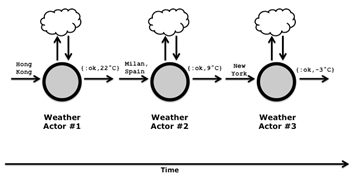
\includegraphics[width=0.8\linewidth]{3_2a.png}
    \caption{没有并发,下一个请求将不得不等待前一个请求完成,这非常低效}
    \label{fig:3_2a}
\end{figure}


需要意识到的一个重要事情是,\emph{每个请求并不依赖于其他请求}。换句话说,我们可以将每个对\texttt{Metex.Worker.temperature\_of/1}的调用打包到一个进程中。让我们教\texttt{Worker}如何响应消息。首先,将\texttt{loop/0}函数添加到\texttt{lib/worker.ex:}

\begin{code}{将loop/0函数添加到\texttt{Worker}中,以便它可以响应消息}
\begin{minted}[linenos]{elixir}
defmodule Metex.Worker do

    def loop do
        receive do
            {sender_pid, location} ->
            send(sender_pid, {:ok, temperature_of(location)})
            _ ->
            IO.puts "don't know how to process this message"
        end
        loop
    end

    defp temperature_of(location) do
    # ...
    end

# ...end
\end{minted}
\label{lst:add_loop_to_worker}
\end{code}

在我们深入了解细节之前,让我们先玩玩这个。如果你已经打开了iex,你可以\emph{重新加载}模块:

\begin{code}{}
\begin{minted}[linenos]{elixir}
iex > r(Metex.Worker)
\end{minted}
% \label{lst:id}
\end{code}

否则,你可以再次运行\texttt{iex -S mix}。首先,我们创建一个运行\texttt{Worker}的循环函数的进程:

\begin{code}{}
\begin{minted}[linenos]{elixir}
iex > pid = spawn(Metex.Worker, :loop, [])
\end{minted}
% \label{lst:id}
\end{code}

内置的spawn函数创建一个进程。spawn有两个版本。第一个版本将一个函数作为参数,第二个版本将一个给定的模块和函数传递给定的参数。两个版本都返回一个\emph{进程id},或者说\emph{pid},作为结果。

\subsection{接收消息}

进程ID(pid)是对进程的\emph{引用},就像在面向对象编程中初始化一个对象会给你一个对该对象的\emph{引用}一样。有了pid,我们就可以向进程发送\emph{消息}。进程可以接收的消息类型在接收块中定义(代码\ref{lst:handlable_message_types}):


\begin{code}{进程可以接收的消息类型在接收块中定义}
\begin{minted}[linenos]{elixir}
receive do
  {sender_pid, location} ->
    send(sender_pid, {:ok, temperature_of(location)})

  _ ->
    IO.puts("don't know how to process this message")
end
\end{minted}
\label{lst:handlable_message_types}
\end{code}

消息是从\emph{上到下}进行模式匹配的。在这种情况下,如果传入的消息是一个两元素元组,那么将执行主体。任何其他消息都将在第二个模式中进行模式匹配。

如果我们将上述代码的函数子句交换顺序,会发生什么呢(代码\ref{lst:message_receive_order_important}):


\begin{code}{模式匹配是从上到下进行的。交换接收到的消息的顺序很重要!}
\begin{minted}[linenos]{elixir}
receive do
_ ->                                  #1
IO.puts "don't know how to process this message"
{sender_pid, location} ->
send(sender_pid, {:ok, temperature_of(location)})
end
#1 这匹配任何消息!
\end{minted}
\label{lst:message_receive_order_important}
\end{code}

如果你试图运行这个,Elixir会有帮助地警告你:
\mintinline{elixir}|{lib/worker.ex:7: warning: this clause cannot match because a previous clause at line 5 always matches}|

换句话说,\mintinline{elixir}|{sender_pid, location}|将\emph{永远不会}被匹配,因为匹配所有操作符(``\texttt{\_"}),顾名思义,将\emph{贪婪地}匹配它所遇到的每一条消息。

一般来说,将匹配所有的情况作为最后一个要匹配的消息是一种好的做法。这是因为未匹配的消息会保留在邮箱中。因此,通过反复向一个不处理未匹配消息的进程发送消息,可能会使虚拟机耗尽内存。

 \subsection{ 发送消息}

消息是使用内置的\texttt{send/2}函数发送的。第一个参数是你想要发送消息的进程的pid。第二个参数是实际的消息。

\begin{code}{\texttt{Worker}可以接收的消息的模式}
\begin{minted}[linenos]{elixir}
receive do
{sender_pid, location} ->               #1
send(sender_pid, {:ok, temperature_of(location)})
end

#1 进入的消息包含发送者pid和位置
\end{minted}
\label{lst:worker_receive_message_pattern}
\end{code}

在这里,我们将请求的结果发送给\texttt{sender\_pid}。我们从哪里得到\texttt{sender\_pid}呢?当然是从进入的消息中!如果你仔细看,我们期望进入的消息由发送者的pid和位置组成。将发送者的pid(或者说任何进程id)放入就像在信封背面放一个\emph{返回地址}一样。它为收件人提供了一个回复的途径。

让我们发送一个消息给我们之前创建的进程(代码\ref{lst:use_send2_send_message}):

\begin{code}{使用send/2向进程发送消息}
\begin{minted}[linenos]{elixir}
iex > send(pid, {self, "Singapore"})
\end{minted}
\label{lst:use_send2_send_message}
\end{code}

结果是\mintinline{elixir}|{#PID<0.125.0>, "Singapore"}|。

等等,除了返回结果,什么都没有发生!让我们稍微分解一下。首先要注意的是,\texttt{send/2}的结果总是\emph{消息}。第二件事是,\texttt{send/2}总是立即返回。换句话说,\texttt{send/2}就像是发射-忘记。所以这就解释了我们是如何得到结果的。但是\emph{为什么}我们没有得到任何结果呢?

我们将什么作为发送者pid传入消息有效载荷?\texttt{self}!\texttt{self}到底是什么?\texttt{self}是调用进程的pid。在这种情况下,它是\texttt{iex}shell会话的pid。我们实际上是告诉\texttt{Worker}将所有的回复发送到shell会话。要从shell会话中获取回复,我们可以使用内置的\texttt{flush/0}函数(代码\ref{lst:useflush0retrieve}):

\begin{code}{使用flush/0检索发送到shell进程的消息}
\begin{minted}[linenos]{elixir}
iex > flush
"Singapore: 27.5°C"
:ok
\end{minted}
\label{lst:useflush0retrieve}
\end{code}

\texttt{flush/0}清除了发送到shell的所有消息并打印它们出来。因此,下次你再做一次\texttt{flush},你只会得到\texttt{:ok}原子。让我们看看这个在实践中是如何工作的。再次,我们有一个城市列表:

\begin{code}{}
\begin{minted}[linenos]{elixir}
iex > cities = ["Singapore", "Monaco", "Vatican City", "Hong Kong", "Macau"]
\end{minted}
% \label{lst:id}
\end{code}

然后,我们遍历每个城市。在每次迭代中,我们生成一个新的\texttt{Worker}。使用新\texttt{Worker}的pid,我们发送一个包含返回地址(\texttt{iex}shell会话)和城市的两元素元组作为消息(\ref{lst:gen_process_each_city}):


\begin{code}{对于每个城市,生成一个进程来查找该城市的温度}
\begin{minted}[linenos]{elixir}
iex >
  cities
  |> Enum.each(fn city ->
    pid = spawn(Metex.Worker, :loop, [])
    send(pid, {self, city})
  end)
\end{minted}
\label{lst:gen_process_each_city}
\end{code}

现在,让我们刷新消息:

\begin{code}{}
\begin{minted}[linenos]{elixir}
iex > flush
{:ok, "Hong Kong: 17.8°C"}
{:ok, "Singapore: 27.5°C"}
{:ok, "Macau: 18.6°C"}
{:ok, "Monaco: 6.7°C"}
{:ok, "Vatican City: 11.8°C"}
:ok
\end{minted}
% \label{lst:id}
\end{code}

太棒了!我们终于得到了我们的结果。注意结果\emph{不是}按任何顺序排列的。这是因为哪个响应先完成就可以在完成后尽快将回复发送回发送者。如果你再次运行迭代,你可能会得到不同顺序的结果。

\begin{figure}[!ht]
    \centering
    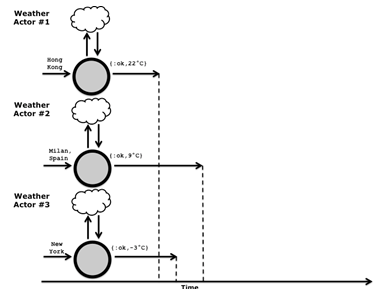
\includegraphics[width=0.8\linewidth]{3_4.png}
    \caption{当进程不必等待彼此时,发送消息的顺序不能保证}
    \label{fig:3_4}
\end{figure}


再看一下 \texttt{loop} 函数。首先要注意的是,它是递归的- 在处理完一条消息后,它会调用自己:

\begin{code}{}
\begin{minted}[linenos]{elixir}
def loop do
  receive do
    {sender_pid, location} ->
      send(sender_pid, {:ok, temperature_of(location)})

    _ ->
      send(sender_pid, "Unknown message")
  end

  # 1
  loop
end

# 1 对loop的递归调用
\end{minted}
% \label{lst:id}
\end{code}

\

你可能会想,为什么我们需要循环。一般来说,进程应该能够处理多于一条的消息。如果我们省略了递归调用,那么进程在处理完第一条(也是唯一的)消息后,就会退出,并被垃圾回收。我们通常希望我们的进程能够处理多于一个的进程!因此,我们需要对消息处理逻辑进行递归调用。

\section{用另一个Actor收集和操作结果}

将结果发送到shell会话对于查看\texttt{Worker}发送的消息很有用,但仅此而已。如果我们想要操作结果,比如说,对它们进行排序,我们需要找到另一种方法。我们可以创建另一个actor来收集结果,而不是使用shell会话作为发送者。

这意味着这个actor必须跟踪\emph{期望的}消息数量。换句话说,actor必须保持状态。我们该如何做呢?

首先,让我们设置actor。创建一个名为\texttt{lib/coordinator.ex}的文件,并按照代码\ref{lst:code_coordinator}中的内容填充它:

\begin{code}{coordinator.ex的完整源代码}
\begin{minted}[linenos]{elixir}
defmodule Metex.Coordinator do
  def loop(results \\ [], results_expected) do
    receive do
      {:ok, result} ->
        new_results = [result | results]

        if results_expected == Enum.count(new_results) do
          send(self, :exit)
        end

        loop(new_results, results_expected)

      :exit ->
        IO.puts(results |> Enum.sort() |> Enum.join(", "))

      _ ->
        loop(results, results_expected)
    end
  end
end
\end{minted}
\label{lst:code_coordinator}
\end{code}

让我们看看我们如何将协调器和\texttt{Worker}一起使用。打开\texttt{lib/metex.ex},并输入以下内容(代码\ref{lst:create_coordinator_worker_process}):


\begin{code}{在lib/metex.ex中创建一个协调器进程和\texttt{Worker}进程的函数}
\begin{minted}[linenos]{elixir}
defmodule Metex do
  def temperatures_of(cities) do
    # 1
    coordinator_pid =
      spawn(Metex.Coordinator, :loop, [[], Enum.count(cities)])

    # 2
    cities
    |> Enum.each(fn city ->
      # 3
      worker_pid = spawn(Metex.Worker, :loop, [])
      # 4
      send(worker_pid, {coordinator_pid, city})
    end)
  end
end

# 1 创建一个协调器进程 
# 2 遍历每个城市 
# 3 创建一个工作进程并执行其循环函数
# 4 向\texttt{Worker}发送一条包含协调器进程pid和城市的消息
\end{minted}
\label{lst:create_coordinator_worker_process}
\end{code}

然后,我们可以通过首先创建一个城市列表来找出城市的温度

\mintinline{elixir}|iex > cities = ["Singapore", "Monaco", "Vatican City", "Hong Kong", "Macau"]|
然后调用Metex.temperatures\_of/1:

\mintinline{elixir}|iex > Metex.temperatures_of(cities)|
结果如预期:

\texttt{Hong Kong: 17.8°C, Macau: 18.4°C, Monaco: 8.8°C, Singapore: 28.6°C, Vatican City: 8.5°C}
这就是\texttt{Metex.temperatures\\\_of/1}的工作原理。首先,我们创建一个协调器进程。协调器进程的循环函数期望两个参数,当前收集的结果和它期望的结果总数。因此,当我们首次创建协调器时,我们用一个初始为空的结果列表和城市数量初始化它:

\mintinline{elixir}|iex > coordinator_pid = spawn(Metex.Coordinator, :loop, [[], Enum.count(cities)])|

现在我们有了等待来自\texttt{Worker}消息的协调器进程。给定一个城市列表,我们遍历每个城市,创建一个\texttt{Worker},然后向\texttt{Worker}发送一条包含协调器pid和城市的消息。

\begin{code}{为每个城市生成工作进程,并将协调器进程设置为\texttt{Worker}消息的接收者}
\begin{minted}[linenos]{elixir}
iex >
  cities
  |> Enum.each(fn city ->
    worker_pid = spawn(Metex.Worker, :loop, [])
    send(worker_pid, {coordinator_pid, city})
  end)
\end{minted}
\label{lst:generate_worker_process_for_each_city}
\end{code}

一旦所有五个\texttt{Worker}完成了请求,协调器将尽职尽责地报告结果:

\texttt{Hong Kong: 16.6°C, Macau: 18.3°C, Monaco: 8.1°C, Singapore: 26.7°C, Vatican City: 9.9°C}
成功!注意结果是按字典顺序排序的。现在是时候深入研究协调器进程,找出它是如何工作的了。

协调器可以从\texttt{Worker}那里接收哪些消息?检查\texttt{receive do ... end}块,我们可以得出至少有两种我们特别感兴趣的消息:

\begin{itemize}
	\item \mintinline{elixir}|{:ok, result}|
  \item \texttt{:exit}
\end{itemize}

其他类型的消息将被忽略。让我们更详细地检查每种消息。

\subsubsection{\{:ok, result\} -顺利进行的消息}

这是我们期望从\texttt{Worker}那里收到的''顺利进行的''消息,如果没有出错的话(代码\ref{lst:successful_message}):


\begin{code}{顺利进行的消息}
\begin{minted}[linenos]{elixir}
def loop(results \\ [], results_expected) do
  receive do
    {:ok, result} ->
      # 1
      new_results = [result | results]
      # 2
      if results_expected == Enum.count(new_results) do
        # 3
        send(self, :exit)
      end

      # 4
      loop(new_results, results_expected)

      # ... 其他模式省略 ...
  end
end

# 1 将结果添加到当前结果列表中
# 2 检查是否已收集到所有结果
# 3 向协调器发送退出消息
# 4 使用新的结果循环。注意,results\_expected保持不变
\end{minted}
\label{lst:successful_message}
\end{code}


当协调器收到符合\mintinline{elixir}|{:ok, result}|模式的消息时,它首先将结果添加到当前的结果列表中。

\begin{figure}[!ht]
    \centering
    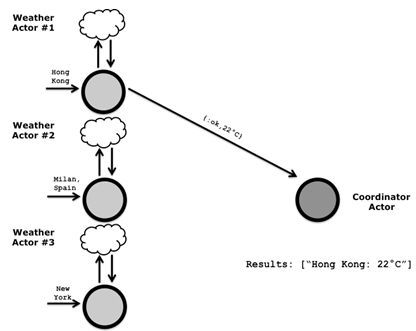
\includegraphics[width=0.8\linewidth]{3_5.png}
    \caption{当第一个结果进入时,actor将结果保存在列表中}
    \label{fig:3_5}
\end{figure}


接下来,我们检查协调器是否已经收到了预期的正确结果数量。假设没有。在这种情况下,循环函数再次调用自己。注意到循环的递归调用的参数。这次我们传入\texttt{new\_results},而\texttt{results\_expected}保持不变。

\begin{figure}[!ht]
    \centering
    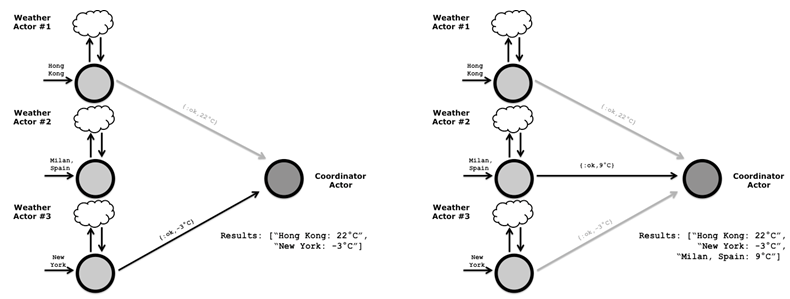
\includegraphics[width=0.8\linewidth]{3_6.png}
    \caption{当协调器收到下一条消息时,它再次将其存储在结果列表中}
    \label{fig:3_6}
\end{figure}

这就是actor中保持状态的方式。参数的\emph{副本}被修改,然后传递到循环函数中,在下一次对自身的函数调用中,它将可用。


\subsection{\texttt{:exit} - 中断信号消息}

当协调器收到所有的消息时,它必须找到一种方法来告诉自己停止,并在必要时报告结果。一种简单的方法是通过一个''中断信号''消息(见代码\ref{lst:break_signal_message})。

\begin{figure}[!ht]
    \centering
    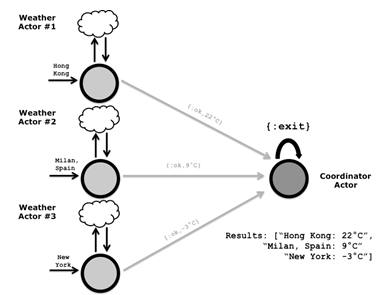
\includegraphics[width=0.8\linewidth]{3_7.png}
    \caption{当协调器收到:exit消息时,它按字母顺序返回结果,然后退出}
    \label{fig:3_7}
\end{figure}

注意,\texttt{:exit}消息本身并不特殊。你可以称之为\texttt{:kill}、\texttt{:self\\\_destruct}或\texttt{:kaboom}。

当协调器收到\texttt{:exit}消息时,它会打印出用逗号分隔的字典顺序的结果。由于我们希望协调器退出,我们不需要调用\texttt{loop}函数。

\begin{code}{中断信号消息}
\begin{minted}[linenos]{elixir}
def loop(results \\ [], results_expected) do
  receive do
    # ... 其他模式省略 ...

    :exit ->
      # 1
      IO.puts(results |> Enum.sort() |> Enum.join(", "))

      # ... 其他模式省略 ...
  end
end

# 1 按字典顺序打印结果,用逗号分隔
\end{minted}
\label{lst:break_signal_message}
\end{code}

\subsection{其他消息}

最后,我们必须处理协调器可能接收到的任何其他类型的消息。我们使用\texttt{\\\_}操作符捕获这些不需要的消息。最后,我们需要记住再次循环,尽管我们保持参数不变(见代码\ref{lst:match_all_other_messages}):

\begin{code}{匹配所有其他消息}
\begin{minted}[linenos]{elixir}
def loop(results \\ [], results_expected) do
  receive do
    # ... 其他模式省略 ...
    # 1
    _ ->
      # 2
      loop(results, results_expected)
  end
end

# 1 匹配所有其他类型的消息

# 2 再次循环,保持参数不变
\end{minted}
\label{lst:match_all_other_messages}
\end{code}


\subsection{宏观视角}

恭喜你 -你刚刚用Elixir编写了你的第一个并发程序!你使用了多个进程来并发地执行计算。在执行计算时,没有一个进程需要等待其他进程,除了协调器进程。

需要强调的一个重要点是,这里没有共享内存。进程内状态的改变只能通过发送消息来实现。这与线程不同,因为线程是共享内存的。这意味着多个线程可以修改同一块内存,这是并发错误(和头痛)的无尽之源。

在设计你自己的并发程序时,决定进程应该接收和发送的消息类型,以及进程之间的交互是很重要的。在我们的示例程序中,我决定使用\mintinline{elixir}|{:ok, result}|和\texttt{:exit}作为协调器进程的消息,使用\mintinline{elixir}|{sender_pid, location}|作为工作进程的消息。我发现,画出各个进程之间的交互以及正在发送和接收的消息是非常有帮助的。抵制直接跳入编码的诱惑,花几分钟时间进行草图绘制。这样做将节省你数小时的挠头和咒骂的时间!

 \section{练习}

进程是Elixir的基础。只有通过运行和实验代码,你才能更好地理解。

\begin{enumerate}
  \item 阅读\texttt{send}和\texttt{receive}的文档。对于\texttt{send},找出你可以发送消息的有效目标。对于\texttt{receive},研究文档提供的示例。\pagenote{http://citeseerx.ist.psu.edu/viewdoc/download?doi=10.1.1.116.1969\&rep=rep1\&type=pdf}
  \item 阅读\texttt{Process}的文档\pagenote{https://www.erlang.org/doc/man/erl\#max\_processes}。
  \item 编写一个程序,生成两个进程。第一个进程,在收到\texttt{ping}消息时,回复一个\texttt{pong}消息。第二个进程,在收到\texttt{pong}消息时,向发送者回复一个\texttt{ping}消息。
\end{enumerate}

 \section{总结}

在本章中,我们介绍了进程这个至关重要的主题。你被介绍到了Actor并发模型。通过示例应用,我们学习了如何:

\begin{enumerate}
  \item 创建进程
  \item 使用进程发送和接收消息
  \item 可以使用多个进程实现并发
  \item 工作进程的消息可以由另一个协调器进程收集和操作
\end{enumerate}

你刚刚尝试了Elixir的并发编程!在做练习的时候玩得开心,一定要给你的大脑稍微休息一下。我们下一章见,我们将学习Elixir的\emph{秘密酱料}
- OTP!

\printnotes*
\chapter{使用GenServer编写服务器应用程序}\label{chapt:genserver}

本章内容包括:

\begin{itemize}

\item  OTP及其使用原因
\item  OTP行为
\item  重写Metex以使用GenServer OTP行为
\item  结构化你的代码以使用GenServer
\item  使用回调处理同步和异步请求
\item  管理服务器状态
\item  干净地停止服务器
\item  为GenServer注册一个名称
\end{itemize}

在本章中,我们首先学习OTP。OTP最初代表Open Telecom Platform。这个名字是由Ericsson的营销天才们创造的(我希望他们不会读到这个!),现在只被称为它的首字母缩写。部分原因是因为这个命名过于短视。OTP提供的工具并不特定于电信领域。然而,这个名字还是被保留下来了,无论好坏。这只是证明了命名确实是计算机科学中最难的问题之一。

我们将学习OTP到底是什么。然后我们将看一下驱动其创建的一些动机。我们还将看到OTP的\emph{行为(Behaviours)}如何帮助我们构建应用程序,减少样板代码,大幅减少潜在的并发错误,并依赖于经过数十年艰苦经验积累的代码。

一旦我们理解了OTP的核心原则,我们将学习一个最重要和最常见的OTP行为 - \texttt{GenServer}。\texttt{GenServer}是Generic Server的简称,\texttt{GenServer}行为是客户端/服务器功能的抽象。我们将把在第3章中构建的温度报告应用程序\texttt{Metex},转变成一个\texttt{GenServer}。到那时,你将对如何实现你自己的\texttt{GenServers}有一个坚实的理解。

 \section{OTP到底是什么?}

OTP有时被称为一个框架,但这并准确。事实上,你应该把OTP看作是一个完整的并发编程开发环境。为了证明我的观点,这里有一个OTP附带功能的非详尽清单:

\begin{itemize}

\item  Erlang解释器和编译器
\item  Erlang标准库
\item  Dialyzer,一个静态分析工具
\item  Mnesia,一个分布式数据库
\item  Erlang Term Storage (ETS),一个内存数据库
\item  一个调试器
\item  一个事件跟踪器
\item  一个发布管理工具
\end{itemize}

我们将在书中的后续部分遇到OTP的各种部分。现在,我们将把注意力转向OTP行为。

 \section{OTP行为}

将OTP行为视为进程的设计模式。这些行为源自经过实战测试的生产代码,并且一直在不断完善。在你的代码中使用OTP行为可以为你提供代码的通用部分,让你只需要实现特定的业务逻辑。

以GenServer为例。GenServer为你提供了开箱即用的客户端/服务器功能。特别是,它提供了所有服务器通用的功能。这些通用功能是什么呢?它们包括:

\begin{itemize}

\item  启动服务器进程
\item  在服务器中维护状态
\item  处理请求并发送回应
\item  停止服务器进程
\end{itemize}

GenServer已经覆盖了通用部分。而你则需要提供业务逻辑。你需要提供的特定逻辑包括:

\begin{itemize}
\item  你想用来初始化服务器的状态
\item  服务器处理的消息类型
\item  何时回复客户端
\item  回复客户端的消息内容
\item  终止后需要清理的资源
\end{itemize}

还有其他的好处。例如,当你正在构建你的服务器应用时,你如何知道你已经覆盖了所有可能出现的必要边缘情况和并发问题呢?此外,理解服务器逻辑的不同实现也不会有趣。

以\texttt{Metex}示例中的\texttt{worker.ex}为例。在我不使用GenServer行为的程序中,我通常将主循环命名为\texttt{loop}。然而,没有人会阻止任何人将其命名为\texttt{await}、\texttt{recur}甚至是像\texttt{while\_1\_true}这样荒谬的名字。使用GenServer行为可以让我(更可能是那些对命名有困难的开发者)免于考虑这些琐事。

\subsection{不同的OTP行为}

下表列出了开箱即用的常见OTP行为。OTP并不限制你只使用这四种。事实上,你可以实现你自己的行为。然而,理解如何正确使用默认的行为是至关重要的,因为它们覆盖了你可能遇到的大多数用例。

\begin{longtable}[]{@{}ll@{}}
\toprule()
行为 & 描述 \\
\midrule()
\endhead
GenServer & 用于实现客户端-服务器关系的服务器的行为模块。 \\
GenEvent & 用于实现事件处理功能的行为模块 \\
Supervisor & 用于实现监督功能的行为模块 \\
Application & 用于处理应用程序和定义应用程序回调的模块。 \\
\bottomrule()
\caption{OTP行为及其提供的功能}
\label{table:otp_behaviours}
\end{longtable}

为了使事情更具体,我们可以亲自看看这些行为是如何组合在一起的。为此,我们需要OTP免费提供的Observer工具。启动\texttt{iex},并启动Observer:

\begin{code}{启动Observer工具}
\begin{minted}[linenos]{elixir}
% iex
iex(1)> :observer.start
:ok
\end{minted}
\label{lst:start_observer}
\end{code}

当窗口弹出时,点击``Applications''选项卡。你应该会看到类似这样的内容:

\begin{figure}[!ht]
    \centering
    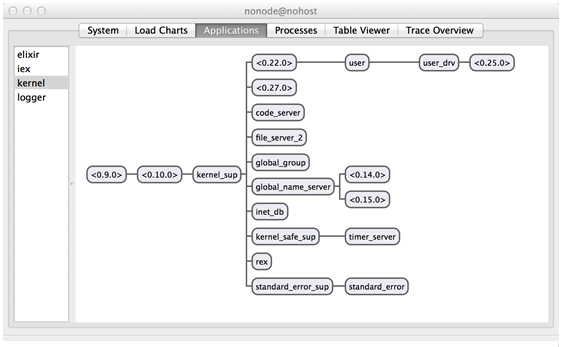
\includegraphics[width=0.8\linewidth]{4_2.png}
    \caption{Observer工具显示Kernel应用的监督器树}
    \label{fig:4_2}
\end{figure}


在左侧列中是一个OTP\emph{应用(Application)}的列表,这些应用在启动iex时已经启动。
我们将在下一章中介绍应用。现在,你可以将它们视为自包含的程序。
点击左列中的每个选项都会显示该应用的\emph{监督器(Supervisor)}层次结构。例如,上图显示了\texttt{kernel}应用的监督器层次结构,这是在\texttt{elixir}应用启动之前就启动的第一个应用。

如果你仔细观察,你会注意到监督器后面都附加了一个\texttt{sup}。例如,\texttt{kernel\_sup}监督了其他十个进程。
这些进程可能是GenServers(例如\texttt{code\_server}和\texttt{file\_server})或者其他的监督器(例如\texttt{kernel\_safe\_sup}和\texttt{standard\_error\_sup})。

像GenServer和GenEvent这样的行为是\emph{工作进程(Worker)} -它们包含了大部分的业务逻辑,并完成了大部分的繁重工作。
随着我们的进展,你将更多地了解它们。
监督器正如它们听起来的那样:它们监督下面的进程,并在发生不好的事情时采取行动。让我们通过从最常用的OTP行为 - GenServer开始,使一切变得更具体。

\section{动手实践OTP:重新审视Metex}

以GenServer为例,我们将实现一个OTP行为。我们将重新实现第\ref{chapt:processes}章中的天气应用\texttt{Metex}。只是这次,我们将使用GenServer行为来实现它。

如果你需要复习一下,\texttt{Metex}会报告给定位置(如城市名称)的摄氏温度。这是通过对第三方天气服务进行HTTP调用来完成的。我们将添加其他的功能,以说明各种GenServer概念,如保持状态和进程注册。例如,我们将跟踪请求的有效位置的频率。

我们将跳过第\ref{chapt:processes}章中讨论的功能部分。换句话说,如果所有这些对你来说都是新的,那么现在将是开始阅读第\ref{chapt:processes}章的最佳时机!
一旦我们完成了应用程序,我们将退一步,比较第\ref{chapt:processes}章和第\ref{chapt:genserver}章的方法。让我们开始吧!

\subsection{创建一个新项目}

像往常一样,创建一个新项目。记住先把你旧版本的\texttt{Metex}放在另一个目录中!

\begin{code}{}
\begin{minted}[linenos]{elixir}
% mix new metex
\end{minted}
% \label{lst:id}
\end{code}

在\texttt{mix.exs}中,填写\texttt{application}和\texttt{deps},如下所示:

\begin{code}{项目设置}
\begin{minted}[linenos]{elixir}
defmodule Metex.Mixfile do
    use Mix.Project

# ...

    def application do
        [applications: [:logger, :httpoison]]
    end

    defp deps do
        [
        {:httpoison, "~> 0.9.0"},
        {:json,      "~> 0.3.0"}
        ]
    end
end
\end{minted}
\label{lst:project_setting_genserver}
\end{code}

然后我们需要获取我们的依赖项。在终端中,使用\texttt{mix deps.get}命令来做到这一点。

\subsection{使Worker符合GenServer}

我们从应用程序的主力,工作进程开始。在\texttt{lib/worker.ex}中,我们首先声明一个新的模块,并指定我们希望使用GenServer行为:

\begin{code}{使用GenServer行为}
\begin{minted}[linenos]{elixir}
defmodule Metex.Worker do
  # 1
  use GenServer
end

# 1 自动定义GenServer所需的所有回调
\end{minted}
\label{lst:use_genserver_behaviour}
\end{code}

只要有\texttt{use GenServer},Elixir就会自动定义GenServer所需的所有回调。这意味着你可以挑选和选择你想要实现的回调。这些回调到底是什么呢?很高兴你问到这个问题。

 \subsection{ 回调}

有六个回调函数会自动为你定义。以下是完整的列表:

\begin{itemize}

\item  \texttt{init(args)}
\item  \texttt{handle\_call(msg, \{from, ref\}, state)}
\item  \texttt{handle\_cast(msg, state)}
\item  \texttt{handle\_info(msg, state)}
\item  \texttt{terminate(reason, state)}
\item  \texttt{code\_change(old\_vsn, state, extra)}
\end{itemize}

在我们进一步讨论之前,有必要提醒自己,我们为什么要费心让工作进程成为一个GenServer,尤其是(如你很快就会看到的)你需要学习各种回调函数和正确的返回值。

使用OTP的最大好处是,当你编写自己的客户端-服务器程序或监督器时,你不必担心的所有事情。例如,你如何编写一个函数来进行异步请求?同步请求呢?GenServer行为为这个确切的用例提供了\texttt{handle\_cast/2}和\texttt{handle\_call/3}。

你的进程必须处理不同类型的消息。随着消息类型的增多,手动编写的进程可能会变得笨重。再次,GenServer的各种\texttt{handle\_*}函数提供了一种整洁的方式来指定你想要处理的不同类型的消息。接收消息只是一半的问题。你还需要一种处理回复的方式。正如预期的那样,回调函数会帮你解决问题,因为它使得访问发送进程的pid变得方便。

现在让我们考虑一下状态管理。每个进程都需要一种初始化状态的方式。它也需要一种在进程终止之前可能进行一些清理的方式。GenServer的\texttt{init/1}和\texttt{terminate/2}就是你需要的回调。

回想一下在上一章中,我们是如何使用递归循环并将(可能)修改过的状态传递给该循环的下一次调用来管理状态的。不同回调的返回值会影响状态。在一个非平凡的进程中手动实现这一点会导致代码看起来很笨拙。

使用GenServer也使得它很容易被插入到比如说,一个监督器中。编写符合OTP行为的程序的好处是,它们看起来往往相似。这意味着,如果你看别人的GenServer,你很可能会很容易地知道它可以处理哪些消息,它可以给出什么回复,以及回复是同步的还是异步的。

现在你知道了只需输入\texttt{use GenServer}就能得到的一些好处。Elixir自动定义了GenServer所需的所有回调。在Erlang中,你需要指定相当多的样板代码。这意味着你可以挑选和选择你想要实现的回调。这些回调到底是什么呢?很高兴你问到这个问题。

\begin{longtable}[]{@{}ll@{}}
\toprule()
GenServer模块调用 & 回调模块(在Metex.Worker中实现) \\
\midrule()
\endhead
\texttt{GenServer.start\_link/3} &
\texttt{Metex.init/1} \\
\texttt{GenServer.call/3} &
\texttt{Metex.handle\_call/3} \\
\texttt{GenServer.cast/2} &
\texttt{Metex.handle\_cast/2} \\
\bottomrule()
\caption{GenServer函数与Metex.Worker的对比}
\label{table:genserver_metex}
\end{longtable}

每个回调都期望一个符合GenServer期望的返回值。下面是一个表格,总结了回调、调用它们的函数以及期望的返回值。当你需要确定每个回调期望的确切返回值时,你会发现这个表格特别有帮助。我发现自己经常参考这个表格。


\begin{longtable}[]{@{}ll@{}}
\toprule()
回调 & 期望的返回值 \\
\midrule()
\endhead
\mintinline{elixir}|init(args)| &
\mintinline{elixir}|{:ok, state}| \\
& \mintinline{elixir}|{:ok, state, timeout}| \\
& \mintinline{elixir}|:ignore| \\
& \mintinline{elixir}|{:stop, reason}| \\
\mintinline{elixir}|handle_call(msg, \{from, ref\},state)| &
\mintinline{elixir}|{:reply, reply, state}| \\
& \mintinline{elixir}|{:reply, reply, state, timeout}| \\
& \mintinline{elixir}|{:reply, reply, state, :hibernate}| \\
& \mintinline{elixir}|{:noreply, state}| \\
& \mintinline{elixir}|{:noreply, state, timeout}| \\
& \mintinline{elixir}|{:noreply, state, hibernate}| \\
& \mintinline{elixir}|{:stop, reason, reply, state}| \\
& \mintinline{elixir}|{:stop, reason, state}| \\
\mintinline{elixir}|handle_cast(msg, state)| &
\mintinline{elixir}|{:noreply, state}| \\
& \mintinline{elixir}|{:noreply, state, timeout}| \\
& \mintinline{elixir}|{:noreply, state, :hibernate}| \\
& \mintinline{elixir}|{:stop, reason, state}| \\
\mintinline{elixir}|handle_info(msg, state)| &
\mintinline{elixir}|{:noreply, state}| \\
& \mintinline{elixir}|{:noreply, state, timeout}| \\
& \mintinline{elixir}|{:stop, reason, state}| \\
\mintinline{elixir}|terminate(reason, state)| &
\mintinline{elixir}|:ok| \\
\mintinline{elixir}|code_change(old_vsn, state, extra)| &
\mintinline{elixir}|{:ok, new_state}| \\
& \mintinline{elixir}|{:error, reason}| \\
\bottomrule()
\caption{GenServer回调及其期望的返回值}
\label{table:genserver_callbacks}
\end{longtable}

当调用\texttt{GenServer.start\_link/3}时,会调用\texttt{init(args)}。让我们在代码中看看:

\begin{code}{用客户端API、服务器回调和辅助函数结构化代码}
\begin{minted}[linenos]{elixir}
defmodule Metex.Worker do
  use GenServer

  ## Client API

  def start_link(opts \\ []) do
    GenServer.start_link(__MODULE__, :ok, opts)
  end

  ## Server Callbacks

  def init(:ok) do
    {:ok, %{}}
  end

  ## Helper Functions
end
\end{minted}
\label{lst:structure_code}
\end{code}

在这里,我通过注释划分了不同的代码部分。你通常会发现野生的Elixir/Erlang程序遵循类似的约定。由于我们还没有引入任何辅助函数,所以``辅助函数''部分被留空。

\subsubsection{\texttt{start\_link/3} 和\texttt{init/1}}

\texttt{GenServer.start\_link/3}接受GenServer实现的模块名,其中定义了\texttt{init/1}回调。它启动进程并将服务器进程链接到父进程。这意味着,如果服务器进程由于某种原因失败,父进程将被通知。

第二个参数是要传递给\texttt{init/1}的参数。由于我们不需要任何参数,所以\texttt{:ok}就足够了。

最后一个参数是要传递给\texttt{GenServer.start\_link/3}的选项列表。这些选项包括定义一个名字来注册进程和启用额外的调试信息。现在,我们可以传入一个空列表。

当调用\texttt{GenServer.start\_link/3}时,它会调用\texttt{Metex.init/1}。它会等待\texttt{Metex.init/1}返回后再返回。\texttt{Metex.init/1}的有效返回值是什么呢?查阅表格,我们得到以下四个值:

\begin{itemize}

\item  \mintinline{elixir}|{:ok, state}|
\item  \mintinline{elixir}|{:ok, state, timeout}|
\item  \texttt{:ignore}
\item  \mintinline{elixir}|{:stop, reason}|
\end{itemize}

现在,我们选择最简单的,\mintinline{elixir}|{:ok state}|。看看我们的实现,这种情况下的\texttt{state}被初始化为一个空的Map,\texttt{\%\{\}}。我们需要这个map来保持请求位置的频率。

让我们试一试!打开你的控制台并启动\texttt{iex}:

\texttt{\% iex -S mix}

现在让我们启动一个服务器进程并将其链接到调用进程。在这种情况下,它是shell进程:

\begin{code}{启动服务器进程}
\begin{minted}[linenos]{elixir}
iex(1)> {:ok, pid} = Metex.Worker.start_link
{:ok, #PID<0.134.0>}
\end{minted}
\label{lst:start_server_process}
\end{code}

结果是一个两元素的元组,和\texttt{:ok}以及新服务器进程的pid。


\subsection{使用 \texttt{handle\_call/3} 处理同步请求}

让我们回到代码。现在,我们希望我们的服务器进程处理请求,这是有服务器进程的全部意义。让我们从客户端API开始,然后向下工作。

\begin{code}{使用 \texttt{GenServer.call/3} 实现同步请求}
\begin{minted}[linenos]{elixir}
defmodule Metex.Worker do
  use GenServer

  ## Client API

  # ...

  def get_temperature(pid, location) do
    GenServer.call(pid, {:location, location})
  end

  ## Server API

  # ...
end
\end{minted}
\label{lst:use_genserver_call}
\end{code}

客户端可能会这样获取新加坡的温度:

\begin{code}{}
\begin{minted}[linenos]{elixir}
Metex.Worker.get_temperature(pid, "Singapore").
\end{minted}
% \label{lst:id}
\end{code}

上述函数包装了对\texttt{GenServer.call/3}的调用,传入pid和一个带有\texttt{:location}标签和实际\texttt{location}的元组。反过来,\texttt{GenServer.call/3}期望在\texttt{Metex.Worker}模块中定义一个\texttt{handle\_call/3}并相应地调用它。

\texttt{GenServer.call/3}向服务器发出\emph{同步}请求。这意味着期望服务器的回复。\texttt{GenServer.call/3}的兄弟是\texttt{GenServer.cast/2},它向服务器发出\emph{异步}请求。我们稍后会看到这个。现在,这是\mintinline{elixir}|{:location, location}|消息的\texttt{handle\_call/3}的实现:


\begin{code}{实现 \texttt{handle\_call} 回调}
\begin{minted}[linenos]{elixir}
defmodule Metex.Worker do
use GenServer

## Client API

# ...

def get_temperature(pid, location) do
GenServer.call(pid, {:location, location})
end

## Server API

# ...

def handle_call(#1{:location, location}, #2_from, #3stats) do
case temperature_of(location) do
{:ok, temp} ->
new_stats = update_stats(stats, location)
{:reply, "#{temp}°C", new_stats}

_ ->
{:reply, :error, stats}
end
end
end

#1: 预期要处理的请求
#2: 这实际上是一个形式为 {pid, tag} 的元组,表示发送者的 pid和消息的唯一引用
#3: GenServer 的当前状态
\end{minted}
\label{lst:use_handle_call}
\end{code}

首先,让我们仔细看一下函数参数:

\begin{code}{}
\begin{minted}[linenos]{elixir}
def handle_call({:location, location}, _from, stats) do
# ...end
\end{minted}
% \label{lst:id}
\end{code}

第一个参数声明了预期要处理的请求。第二个参数返回一个形式为\mintinline{elixir}|{pid, tag}|的元组,其中\texttt{pid}是客户端的pid,\texttt{tag}是消息的唯一引用。第三个参数,\texttt{state},表示服务器的\emph{内部状态}。在我们的情况下,它是当前有效位置的频率计数。

现在,让我们关注\mintinline{elixir}|handle_call({:location, location}, ...)|的主体:

\begin{code}{}
\begin{minted}[linenos]{elixir}
def handle_call({:location, location}, _from, stats) do
    case temperature_of(location) do              #1
        {:ok, temp} ->
            new_stats = update_stats(stats, location) #2
            {:reply, "#{temp}°C", new_stats}          #3

        _ -> {:reply, :error, stats}                   #3
    end
end

#1: 向 API 请求位置的温度 
#2: 使用位置频率更新Map stats  
#3: 返回一个作为响应的三元素元组。
\end{minted}
% \label{lst:id}
\end{code}



\texttt{Metex.Worker.temperature\_of/1}向第三方API发出请求,以获取位置的温度。
如果成功,\texttt{Metex.Worker.update\_stats/2}被调用,返回一个带有更新的位置频率的新Map。
最后,它返回一个任何\texttt{handle\_call/3}都期望返回的三元素元组。

特别是,这个三元组以\texttt{:reply}开始,然后是实际计算的响应,然后是更新的状态,这种情况下是\texttt{new\_stats}。
如果出于某种原因向第三方API的请求失败,那么将返回\mintinline{elixir}|{:reply, :error, stats}|。以下是\texttt{handle\_call/3}的有效响应:

\begin{itemize}

\item  \mintinline{elixir}|{:reply, reply, state}|
\item  \mintinline{elixir}|{:reply, reply, state, timeout}|
\item  \mintinline{elixir}|{:reply, reply, state, :hibernate}|
\item  \mintinline{elixir}|{:noreply, state}|
\item  \mintinline{elixir}|{:noreply, state, timeout}|
\item  \mintinline{elixir}|{:noreply, state, hibernate}|
\item  \mintinline{elixir}|{:stop, reason, reply, state}|
\item  \mintinline{elixir}|{:stop, reason, state}|
\end{itemize}

让我们填补一下缺失的部分,以便让\texttt{Metex.Worker.get\_temperature/2}工作:

\begin{code}{实现辅助函数}
\begin{minted}[linenos]{elixir}
defmodule Metex.Worker do
  use GenServer

  ## Client API and Server API

  ## previously implemented code

  ## Helper Functions

  defp temperature_of(location) do
    url_for(location) |> HTTPoison.get() |> parse_response
  end

  defp url_for(location) do
    "http://api.openweathermap.org/data/2.5/weather?q=#{location}&APPID=#{apikey}"
  end

  defp parse_response({:ok, %HTTPoison.Response{body: body, status_code: 200}}) do
    body |> JSON.decode!() |> compute_temperature
  end

  defp parse_response(_) do
    :error
  end

  defp compute_temperature(json) do
    try do
      temp = (json["main"]["temp"] - 273.15) |> Float.round(1)
      {:ok, temp}
    rescue
      _ -> :error
    end
  end

  def apikey do
    "APIKEY-GOES-HERE"
  end

  defp update_stats(old_stats, location) do
    case Map.has_key?(old_stats, location) do
      true ->
        Map.update!(old_stats, location, &(&1 + 1))

      false ->
        Map.put_new(old_stats, location, 1)
    end
  end
end
\end{minted}
\label{lst:helper_functions}
\end{code}

大部分的实现与第\ref{chapt:processes}章相同,只是对\texttt{Metex.Worker.temperature\_of/1}和\texttt{Metex.Worker.update\_stats/2}做了一些小的修改,这两个函数是全新的。
\texttt{Metex.Worker.update\_stats/2}的实现非常简单:

\begin{code}{更新请求位置的频率}
\begin{minted}[linenos]{elixir}
defp update_stats(old_stats, location) do
  case Map.has_key?(old_stats, location) do
    true ->
      Map.update!(old_stats, location, &(&1 + 1))

    false ->
      Map.put_new(old_stats, location, 1)
  end
end
\end{minted}
\label{lst:update_stats}
\end{code}

这个函数接收\texttt{old\_stats}和请求的\texttt{location}。我们首先检查\texttt{old\_stats}是否包含位置的键。如果是,我们可以简单地获取值并增加计数器。否则,我们放入一个由\texttt{location}表示的新键,并将其设置为\texttt{1}。如果\texttt{\&(\&1 + 1)}的匿名函数写法看起来让人困惑,你可以在你的脑海中进行语法``去糖化'':

\begin{code}{}
\begin{minted}[linenos]{elixir}
Map.update!(old_stats, location, fn val -> val + 1 end)
\end{minted}
% \label{lst:id}
\end{code}

让我们再次尝试一下\texttt{Metex.Worker}。再次启动\texttt{iex},然后使用\texttt{Metex.Worker.start\_link/1}启动服务器:

\begin{code}{}
\begin{minted}[linenos]{elixir}
% iex -S mix
iex(1)> {:ok, pid} = Metex.Worker.start_link
{:ok, #PID<0.125.0>}
\end{minted}
% \label{lst:id}
\end{code}

现在,让我们从一些著名的地点获取温度:

\begin{code}{}
\begin{minted}[linenos]{elixir}
iex(2) > Metex.Worker.get_temperature(pid, "Babylon")
"12.7°C"
iex(3) > Metex.Worker.get_temperature(pid, "Amarillo")
"5.3°C"
iex(4) > Metex.Worker.get_temperature(pid, "Memphis")
"7.3°C"
iex(5) > Metex.Worker.get_temperature(pid, "Rio")
"23.5°C"
iex(6) > Metex.Worker.get_temperature(pid, "Philadelphia")
"12.5°C"
\end{minted}
% \label{lst:id}
\end{code}


\subsection{访问服务器状态}

成功了!但等一下,我如何查看\texttt{stat}的内容呢?换句话说,我们如何访问\emph{服务器状态}?事实证明,这并不难。让我们首先实现面向客户端的API:

\begin{code}{}
\begin{minted}[linenos]{elixir}
def get_stats(pid) do
  GenServer.call(pid, :get_stats)
end
\end{minted}
% \label{lst:id}
\end{code}

由于我们期望服务器的回复,我们需要服务器的同步回复。因此,我们应该调用\texttt{GenServer.call/3}。在这里,我们说服务器应该处理一个同步的\texttt{:get\_stats}消息。注意,消息可以是任何有效的Elixir项的形式。这意味着元组、列表和原子都是合法的返回值。这是回调函数:

\begin{code}{}
\begin{minted}[linenos]{elixir}
def handle_call(:get_stats, _from, stats) do
  {:reply, stats, stats}
end
\end{minted}
% \label{lst:id}
\end{code}

由于我们对\texttt{stats}感兴趣,我们可以在第二个参数中简单地返回\texttt{stats}作为回复。由于我们只是访问\texttt{stats},而不是修改它,我们简单地将其保持不变作为第三个参数。

在我们继续之前,这里有一个温馨的提醒,要\emph{将所有的\texttt{handle\_call}(以及稍后的\texttt{handle\_cast})分组在一起}!这很重要,因为Erlang虚拟机依赖于这个进行模式匹配。例如,如果我''误放''了\texttt{handle\_call},就像这样:

\begin{code}{注意 \texttt{handle\_calls} 没有分组在一起}
\begin{minted}[linenos]{elixir}
defmodule Metex.Worker do
  use GenServer

  ## Client API

  # ...

  ## Server Callbacks

  # 1
  def handle_call(:get_stats, _from, stats) do
    # ...
  end

  def init(:ok) do
    # ...
  end

  def handle_call({:location, location}, _from, stats) do
    # ...
  end

  ## Helper Functions

  # ...
end

# 1: handle_calls 和 handle_casts 应该分组在一起
\end{minted}
\label{lst:note_handle_calls}
\end{code}

然后,编译器会发出一个友好的警告:

\begin{code}{}
\begin{minted}[linenos]{elixir}
% iex -S mix
lib/worker.ex:29: warning: clauses for the same def should be grouped together, def handle_call/3 was previously defined (lib/worker.ex:20)
\end{minted}
% \label{lst:id}
\end{code}


\subsection{使用 \texttt{handle\_cast/2} 处理异步请求}

异步请求不需要服务器的回复。这也意味着\texttt{GenServer.cast/2}会立即返回。对于\texttt{GenServer.cast/2}来说,什么是一个好的用例呢?一个很好的例子是向服务器发出一个命令,这个命令会在服务器的状态中产生一些副作用。在这种情况下,发出命令的客户端不应该关心回复。

让我们构造这样一个命令。这个命令叫做\texttt{reset\_stats},它将把stats重新初始化为一个空的Map:

\begin{code}{处理重置统计}
\begin{minted}[linenos]{elixir}
# Client API

# ...

def reset_stats(pid) do
  GenServer.cast(pid, :reset_stats)
end

# Server Callbacks

# handle_calls go here

def handle_cast(:reset_stats, _stats) do
  {:noreply, %{}}
end
\end{minted}
\label{lst:hangle_reset_stats}
\end{code}

\texttt{Metex.Worker.stats/1}将调用\texttt{GenServer.cast/2}。这反过来又调用了\texttt{handle\_cast(:reset\_stats, \_stats)}回调。由于我们不关心服务器的当前状态(毕竟,我们正在重置它),我们在\texttt{stats}前面加上一个下划线。

返回值是一个两元素的元组,第一个元素是\texttt{:noreply},第二个元素是一个空的Map,也就是响应。再次注意,响应是有效的\texttt{handle\_cast/2}响应之一。

让我们看看我们的成果!再次启动\texttt{iex -S mix},然后尝试一些位置:

\begin{code}{}
\begin{minted}[linenos]{elixir}
iex(1)> {:ok, pid} = Metex.Worker.start_link
{:ok, #PID<0.134.0>}
iex(2)> Metex.Worker.get_temperature pid, "Singapore"
"29.0°C"
iex(3)> Metex.Worker.get_temperature pid, "Malaysia"
"22.7°C"
iex(4)> Metex.Worker.get_temperature pid, "Brunei"
"24.2°C"
iex(5)> Metex.Worker.get_temperature pid, "Singapore"
"29.0°C"
iex(6)> Metex.Worker.get_temperature pid, "Cambodia"
"27.7°C"
iex(7)> Metex.Worker.get_temperature pid, "Brunei"
"24.2°C"
iex(8)> Metex.Worker.get_temperature pid, "Singapore"
"29.0°C"
\end{minted}
% \label{lst:id}
\end{code}

现在我们可以尝试一下 \texttt{get\_stats/1} 函数:

\begin{code}{}
\begin{minted}[linenos]{elixir}
iex(9) > Metex.Worker.get_stats(pid)
%{"Brunei" => 2, "Cambodia" => 1, "Malaysia" => 1, "Singapore" => 3}
\end{minted}
% \label{lst:id}
\end{code}

它工作了!你可以清楚地看到由Map表示的请求位置的频率。现在,让我们试着重置\texttt{stats}:

\begin{code}{}
\begin{minted}[linenos]{elixir}
iex(10) > Metex.Worker.reset_stats(pid)
:ok
iex(11) > Metex.Worker.get_stats(pid)
%{}
\end{minted}
% \label{lst:id}
\end{code}

完美!它按预期工作了。


\subsection{停止服务器并清理}

有时,我们需要在服务器停止之前释放资源,或者进行一些其他的清理任务。这就是\texttt{GenServer.terminate/2}的作用。

那么我们如何停止服务器呢?如果你查看回调表,在\texttt{handle\_call/handle\_cast}列下,你会发现两个以\texttt{:stop}开头的有效响应:

\begin{itemize}
\item  \mintinline{elixir}|{:stop, reason, new_state}|
\item  \mintinline{elixir}|{:stop, reason, reply, new_state}|
\end{itemize}

这是一个信号,告诉GenServer服务器将被终止。因此,我们需要做的就是提供一个返回上述响应的任意一个的回调(来自\texttt{handle\_call/3}或\texttt{handle\_cast/2}),并在\texttt{GenServer.terminate/2}回调中包含清理逻辑。我们首先在客户端API下写一个\texttt{stop/1}函数:

\begin{code}{}
\begin{minted}[linenos]{elixir}
def stop(pid) do
  GenServer.cast(pid, :stop)
end
\end{minted}
% \label{lst:id}
\end{code}

再次,我选择了\texttt{GenServer.cast/2},因为我并不真正关心任何返回值。另一个原因可能是服务器可能需要时间来正确地清理所有资源,而我不想等待。相应的回调非常简单:

\begin{code}{}
\begin{minted}[linenos]{elixir}
def handle_cast(:stop, stats) do
  {:stop, :normal, stats}
end
\end{minted}
% \label{lst:id}
\end{code}

我们没有任何资源可以说的,但你可以想象我们可能会例如将\texttt{stats}写入文件或数据库。在我们的例子中,让我们在停止服务器之前打印当前状态:

\begin{code}{终止回调在服务器终止之前被调用}
\begin{minted}[linenos]{elixir}
def terminate(reason, stats) do
  # 我们可以写入文件、数据库等
  IO.puts("server terminated because of #{inspect(reason)}")
  inspect(stats)
  :ok
end
\end{minted}
\label{lst:stop_callback_before_server_terminates}
\end{code}

\texttt{GenServer.terminate/2}有两个参数。第一个参数提供了服务器终止的原因。在正常终止时,原因将是\texttt{:normal}。\texttt{:normal}来自早期定义的\texttt{handle\_cast/2}的响应。对于错误,例如由于捕获到的异常,你可以包含其他原因。最后,\texttt{GenServer.terminate/2}必须始终返回\texttt{:ok}。让我们看看我们如何在iex中终止一个服务器。

\begin{code}{}
\begin{minted}[linenos]{elixir}
% iex -S mix
iex(1)> {:ok, pid} = Metex.Worker.start_link
{:ok, #PID<0.152.0>}
iex(2)> Process.alive? pid
true
iex(3)> Metex.Worker.stop pid
server terminated because of :normal
:ok
iex(4)> Process.alive? pid
false
\end{minted}
% \label{lst:id}
\end{code}


\subsection{当回调返回无效响应时会发生什么?}

让我们稍微修改一下\texttt{handle\_cast(:stop, stats)}的返回值:

\begin{code}{}
\begin{minted}[linenos]{elixir}
def handle_cast(:stop, stats) do
  {:stop, :normal, :ok, stats}
end
\end{minted}
% \label{lst:id}
\end{code}

如果你再看一下表格,这对应于一个有效的\texttt{handle\_call/3}响应,而不是\texttt{handle\_cast/2}!多余的\texttt{:ok}是为了回复客户端。由于\texttt{handle\_cast/2}并不是为了回复客户端(至少,不是直接回复),所以这显然是错误的。让我们看看当我们重复停止服务器的过程时会发生什么:


\begin{code}{当回调没有返回预期的响应时,GenServer会报错}
\begin{minted}[linenos]{elixir}
% iex -S mix
iex(1)> {:ok, pid} = Metex.Worker.start_link
{:ok, #PID<0.152.0>}
iex(2)> Metex.Worker.stop pid
iex(2)>
10:59:15.906 [error] GenServer #PID<0.134.0> terminating #1
Last message: {:"$gen_cast", :stop}                      #1
State: %{}                                               #1
** (exit) bad return value: {:stop, :normal, :ok, %{}}   #1
#1 GenServer在收到回调处理器的无效响应时报告错误
\end{minted}
\label{lst:invalid_response}
\end{code}

首先,注意到这里\emph{没有}编译时错误。只有当我们试图停止服务器时,错误才会浮出水面,GenServer会抛出一个
\mintinline{elixir}|{bad return value: {:stop, :normal, :ok, %{}}}|。
每当你看到这样的东西,你的第一反应应该是仔细检查你的回调处理器的返回值。有时候很容易忽略一些小细节,而且错误信息一开始可能并不那么明显。


\subsection{接收其他类型的消息}

可能会有来自其他进程的消息,这些消息可能没有在\texttt{handle\_call/3}/\texttt{handle\_cast/2}中定义。这就是\texttt{handle\_info/2}的作用。它被调用来处理进程接收到的任何其他消息,有时被称为``带外''消息。你不需要为\texttt{handle\_info/2}提供一个客户端API对应项。这个回调接收两个参数,接收到的消息和当前的状态:

\begin{code}{}
\begin{minted}[linenos]{elixir}
def handle_info(msg, stats) do
  IO.puts("received #{inspect(msg)}")
  {:noreply, stats}
end
\end{minted}
% \label{lst:id}
\end{code}

让我们看看这个在实践中的应用:


\begin{code}{有了 \texttt{handle\_info},服务器进程可以处理任何类型的意外消息}
\begin{minted}[linenos]{elixir}
iex(1)> {:ok, pid} = Metex.Worker.start_link
{:ok, #PID<0.134.0>}
iex(2)> send pid, "It's raining men"
received "It's raining men"
\end{minted}
\label{lst:handle_info_can_handle_any_type_of_message}
\end{code}

我们将在后面的章节中看到更多有趣的\texttt{handle\_info/2}的用途。主要要记住的是,\texttt{handle\_info/2}用于处理任何其他不被\texttt{handle\_call/3}/\texttt{handle\_cast/2}覆盖的消息。

 \subsection{进程注册}

不断通过pid引用GenServer可能会很痛苦。幸运的是,还有另一种方法可以做到这一点。\texttt{GenServer.start\_link/3}接受一个选项列表作为它的第三个参数。

有两种常见的方式可以用一个名字注册一个GenServer,区别在于名字应该在本地还是全局可见。
如果名字被全局注册,那么名字在连接的节点集群(你将很快了解到分布式集群)中是唯一的。
另一方面,本地注册的名字只在本地节点内可见。

对于单例GenServer来说,有一个注册的名字是很好的。也就是说,只应该在一个节点或集群中存在一个。我们将让\texttt{Metex.Worker}在\texttt{MW}下注册。当我们选择为GenServer注册一个名字时,我们就不再需要使用它的pid来引用进程。幸运的是,我们只需要改变客户端API中对\texttt{GenServer.call/3}和\texttt{GenServer.cast/2}的调用:

\begin{code}{有了一个明确的名字,就不再需要将pid传递给客户端API}
\begin{minted}[linenos]{elixir}
defmodule Metex.Worker do
  use GenServer

  # 1
  @name MW

  ## Client API

  def start_link(opts \\ []) do
    # 2
    GenServer.start_link(__MODULE__, :ok, opts ++ [name: MW])
  end

  def get_temperature(location) do
    # 3
    GenServer.call(@name, {:location, location})
  end

  def get_stats do
    # 3
    GenServer.call(@name, :get_stats)
  end

  def reset_stats do
    # 3
    GenServer.cast(@name, :reset_stats)
  end

  def stop do
    # 3
    GenServer.cast(@name, :stop)
  end

  # The rest of the code remains unchanged.
  # ...
end

# 1 存储名字
# 2 用一个注册的名字初始化服务器
# 3 注意我们传递的是 @name 而不是 pid
\end{minted}
\label{lst:with_a_named_server_we_no_longer_need_to_pass_pids_to_the_client_api}
\end{code}


现在,再次启动\texttt{iex -S mix}。这次,我们不需要显式地捕获pid。然而,这是一个好主意,因为我们通常想知道服务器是否正确启动,因此我们希望确保匹配到\texttt{:ok}。

现在,我们可以这样与\texttt{Metex.Worker}交互:

\begin{code}{}
\begin{minted}[linenos]{elixir}
% iex -S mix
iex(1)> Metex.Worker.start_link
{:ok, #PID<0.134.0>}
iex(2)> Metex.Worker.get_temperature "Singapore"
"29.3°C"
iex(3)> Metex.Worker.get_temperature "London"
"2.0°C"
iex(4)> Metex.Worker.get_temperature "Hong Kong"
"24.0°C"
iex(5)> Metex.Worker.get_temperature "Singapore"
"29.3°C"
iex(6)> Metex.Worker.get_stats
%{"Hong Kong" => 1, "London" => 1, "Singapore" => 2}
iex(7)> Metex.Worker.stop
server terminated because of :normal
:ok
\end{minted}
% \label{lst:id}
\end{code}


\subsection{回顾第3章的Metex}

再看一下我们在第\ref{chapt:processes}章中构建的\texttt{Metex}。试着想象一下我们需要添加什么才能获得与本章中构建的\texttt{Metex}相同的功能。另外,试着想象一下你会把所有这些功能放在哪里。

你可能会意识到,有些功能并不容易实现。例如,你如何实现同步和异步调用?停止服务器呢?在这种情况下,我们必须特别处理停止消息,而不是运行循环。那么我们应该在哪里放置清理资源的逻辑呢?

在早期版本的\texttt{Metex.Worker}中,我们必须在循环中使用通配符操作符(即下划线)显式处理意外消息。在OTP中,这是通过\texttt{handle\_info/2}回调处理的。服务器的停止也没有被处理。

考虑到所有这些问题,你很快就会意识到循环函数的大小会开始膨胀。当然,你总是可以把所有的东西抽象出来,放在漂亮的小函数中,但这只能做到一定程度。

希望你能开始看到OTP的好处。使用OTP行为可以帮助你在代码中获得一致的结构。它使你能够轻松地看到客户端API在哪里,服务器回调是如何定义的,以及辅助方法在哪里。

除了提供一致性,OTP还提供了许多对所有类似服务器的程序都有用的功能。例如,使用GenServer管理状态非常简单。你不再需要将你的状态放在一个循环中。能够在回调中决定何时改变你的状态也非常有用。

 \section{练习}

编写一个GenServer,可以存储任何有效的Elixir项,给定一个键。以下是一些可以让你开始的操作:

\begin{itemize}
\item  \texttt{Cache.write(:stooges, ["Larry", "Curly", "Moe"])}
\item  \texttt{Cache.read(:stooges)}
\item  \texttt{Cache.delete(:stooges)}
\item  \texttt{Cache.clear}
\item  \texttt{Cache.exist?(:stooges)}
\end{itemize}

按照我们在本章中的方式来构造你的程序。特别注意上述哪些操作应该是\texttt{handle\_call}或\texttt{handle\_cast}。

\section{总结}

当我第一次学习GenServer时,我需要接受很多信息------这还是轻描淡写的说法。下面的表格可以帮助你将所有相关的函数分组在一起。

我缩写了一些函数名,将\texttt{Metex.Worker}缩写为\texttt{MW},将\texttt{GenServer}缩写为\texttt{GS}。\texttt{state}被缩短为\texttt{st},\texttt{from}被缩短为\texttt{fr}。最后,\texttt{pid}是\texttt{p}。


\begin{longtable}[]{@{}
  >{\raggedright\arraybackslash}p{(\columnwidth - 4\tabcolsep) * \real{0.3333}}
  >{\raggedright\arraybackslash}p{(\columnwidth - 4\tabcolsep) * \real{0.3333}}
  >{\raggedright\arraybackslash}p{(\columnwidth - 4\tabcolsep) * \real{0.3333}}@{}}
\toprule()
\begin{minipage}[b]{\linewidth}\raggedright
Metex.Worker 客户端API
\end{minipage} & \begin{minipage}[b]{\linewidth}\raggedright
GenServer
\end{minipage} & \begin{minipage}[b]{\linewidth}\raggedright
Metex.Worker 回调
\end{minipage} \\
\midrule()
\endhead
\mintinline{elixir}|MW.start_link(:ok)| &
\mintinline{elixir}|GS.start_link| &
\mintinline{elixir}|MW.init(:ok)| \\
\mintinline{elixir}|MW.get_temp(p,"NY")| &
\mintinline{elixir}|GS.call(p,{:loc,"NY"})| &
\mintinline{elixir}|MW.handle_call({:loc, "NY"}, fr, st)| \\
\mintinline{elixir}|MW.reset(p)| &
\mintinline{elixir}|GS.cast(p, :reset)| &
\mintinline{elixir}|MW.handle_cast(:reset, st)| \\
\mintinline{elixir}|MW.stop(p)| &
\mintinline{elixir}|GS.cast(p, :stop)| &
\mintinline{elixir}|MW.handle_cast(:stop, st)| \\
& & 如果上述返回\mintinline{elixir}|{:stop, :normal, st}| \\
& & 那么 \\
& & \mintinline{elixir}|MW.terminate(:normal, st)| 将被调用 \\
\bottomrule()
\caption{客户端API、GenServer和回调函数之间关系的总结}
\label{table:summary_of_the_relationship_between_the_client_api_genserver_and_the_callbacks}
\end{longtable}

让我们看一下最后一行。假设我想停止工作进程,我调用\texttt{Metex.Worker.stop/1}。这将反过来调用\texttt{GenServer.cast/2},传入\texttt{pid}和\texttt{:stop}作为参数。触发的回调将是\texttt{Metex.Worker.handle\_cast(:stop, state)}。如果回调返回一个形如\mintinline{elixir}|{:stop, :normal, state}|的元组,那么就会调用\texttt{Metex.Worker.terminate/2}。

在本章中,我们涵盖了很多内容。以下是一些重点:

\begin{itemize}

\item  OTP是什么,以及其背后的原则和动机
\item  可用的不同类型的OTP行为
\item  将Metex转换为使用GenServer
\item  GenServer提供的各种回调
\item  在GenServer中管理状态
\item  按照约定结构化你的代码
\item  进程注册
\end{itemize}

还有一个好处,我一直故意没有告诉你。使用GenServer行为可以让你将GenServers放入一个监督树中。如果你的GenServer崩溃了会发生什么?它将如何影响你系统的其他部分,你如何确保你的系统保持功能?

请继续阅读,亲爱的读者,因为接下来是监督器------这恰好是我最喜欢的OTP特性之一!


%Part 2
\part{容错、监督与分布式处理}\label{part2}

我们现在进入了大多数语言和平台难以处理的领域,即容错和分布式处理。我们将学习Erlang虚拟机(Erlang VM)提供的基本工具,用于检测进程何时崩溃。

接着,我们将学习第二种OTP行为------监督器(Supervisor),以及如何管理进程的层级结构,并在进程崩溃时自动采取行动。我们专门用两章来构建一个功能完备的工作池应用程序,该程序利用了通用服务器(GenServers)和监督器。

在接下来的两章中,我们将通过负载平衡和容错的视角来研究分布式处理。在这两章的学习结束时,你将构建出一个分布式的负载测试器,一个分布式且具备容错能力的Chuck Norris笑话服务。更重要的是,你将掌握如何有效使用OTP。

\chapter{并发错误处理和容错性:链接、监视器和进程}\label{chapt:concurrent}

本章内容包括:

\begin{itemize}

\item  以 Elixir 风格处理错误
\item  链接、监视器和捕获退出
\item  实现一个监督器
\end{itemize}

是否看过阿诺德·施瓦辛格主演的《终结者》?那部关于未来的刺客机器人的电影?无论终结者受到多少枪击,它总能不屈不挠地一次又一次地复原。在本章结束时,你将熟悉容错性功能,能够构建能够优雅处理错误并采取纠正措施解决问题的程序。当然,你至少目前还无法构建天网。

在顺序程序中,通常只有一个主进程在做所有繁重的工作。如果这个进程崩溃了怎么办?通常,这意味着整个程序都崩溃了。常见的处理方法是进行\emph{防御性编程}。这通常意味着在程序中加入\texttt{try}、 \texttt{catch} 和\texttt{if err != nil}。

但在构建并发程序时,情况就不同了。由于有不止一个进程在运行,所以有可能\emph{另一个}进程\emph{检测到崩溃}并随后\emph{处理错误}。这是一个非常解放性的概念。

你可能听说过或读过 Erlang 的非官方座右铭------``让它崩溃''------Erlang程序员非常喜欢这么说。因为这是 Erlang VM中处理事务的方式。事实证明,这么做有几个很好的理由,我们很快就会了解到。这种独特的错误处理方式可能会让习惯了防御性编程的程序员不由自主地抽搐。

在本节中,我们将首先了解\emph{链接}、\emph{监视器}、\emph{捕获退出}和\emph{进程},以及它们如何共同构成构建容错系统的基础构建块。然后我们将开始构建一个简单版本的监督器,其唯一的工作是管理工作进程。这将是进入下一章的完美过渡,在那里我们可以更充分地欣赏
OTP 监督器行为所提供的便利和附加功能。

\section{链接 ---直到死亡将我们分开}

当一个进程链接到另一个进程时,它创建了一个双向关系。链接的进程有一个\emph{链接集},其中包含它所链接的所有进程的集合。如果任一进程因任何原因终止,一个\emph{退出信号}会传播到所有与它链接的进程。此外,如果这些进程中的任何一个链接到不同的进程集,那么\emph{相同}的退出信号也会沿着传播。

\begin{figure}[!ht]
    \centering
    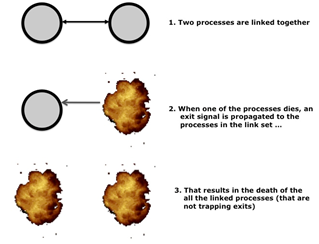
\includegraphics[width=0.8\linewidth]{5_1.png}
    \caption{当一个进程死亡时,所有链接到它的其他进程也将死亡(假设它们没有捕获退出)}
    \label{fig:5_1}
\end{figure}


如果你现在在挠头并想知道为什么这是件好事,请考虑以下示例,一群进程在进行map-reduce作业。如果这些进程中的任何一个崩溃并死亡,让其余进程继续工作就没有意义了。事实上,让进程相互链接将简化剩余进程的清理工作,因为其中一个进程的失败会自动导致其余链接的进程崩溃。


\subsection{将进程链接在一起}

为了理解这一点,需要一个示例。使用\texttt{Process.link/1}创建链接,唯一的参数是要\emph{链接到}的进程的进程 ID。这意味着\texttt{Process.link/1} 必须在现有进程中调用。

\texttt{Process.link/1} 和\texttt{Process.monitor/1} 都是在进程的上下文中调用的

注意 \texttt{Process.link/1}必须在现有的进程中调用,因为没有\texttt{Process.link(link\_from, link\_to)}这样的东西。\texttt{Process.monitor/1} 也是如此。

打开一个 \texttt{iex} 会话。我们将创建一个与\texttt{iex} shell 进程链接的进程。由于我们处于 shell进程的上下文中,所以每当我们调用\texttt{Process.link/1} 时,我们都将 shell进程链接到我们指向的任何进程。

我们要创建的进程将在接收到 \texttt{:crash}消息时崩溃。观察它崩溃时会发生什么。首先,让我们记录下当前 shell 进程的pid:

\begin{code}{}\begin{minted}[linenos]{elixir}
iex > self
# PID<0.119.0>
\end{minted}
% \caption{Listing Caption}
% \label{lst:id}
\end{code}

我们可以检查当前 shell 进程的链接集:

\begin{code}{}
\begin{minted}[linenos]{elixir}
iex > Process.info(self, :links)
{:links, []}
\end{minted}
% \label{lst:id}
\end{code}

\texttt{Process.info/1}包含有关进程的许多其他有用信息。我们使用\texttt{Process.info(self, :links)}是因为我们现在只对链接集感兴趣。其他有趣的信息包括邮箱中的消息总数、堆大小以及进程启动时的参数。

正如预期的那样,它是空的,因为我们还没有链接任何进程。接下来,让我们创建一个只对\texttt{:crash} 消息作出响应的进程:

\begin{code}{}
\begin{minted}[linenos]{elixir}
iex > pid =
  spawn(fn ->
    receive do
      :crash -> 1 / 0
    end
  end)

# PID<0.133.0>
\end{minted}
% \label{lst:id}
\end{code}

现在,我们将 shell 进程链接到我们刚刚创建的进程:

\begin{code}{}
\begin{minted}[linenos]{elixir}
iex > Process.link(pid)
\end{minted}
% \label{lst:id}
\end{code}

\texttt{<0.133.0>} 现在在\texttt{self} 的链接集中:

\begin{code}{}
\begin{minted}[linenos]{elixir}
iex> Process.info(self, :links)
{:links, [#PID<0.133.0>]}
\end{minted}
% \label{lst:id}
\end{code}

反过来,\texttt{self}(\texttt{<0.119.0>}) 也在\texttt{<0.133.0>} 的链接集中:

\begin{code}{}
\begin{minted}[linenos]{elixir}
iex> Process.info(pid, :links)
{:links, [#PID<0.119.0>]}
\end{minted}
% \label{lst:id}
\end{code}

现在应该很清楚了,从 shell 进程中调用\texttt{Process.link/1} 创建了一个双向链接,将 shell进程和我们刚刚产生的进程链接在一起。

现在,我们一直在等待的时刻到了------让我们结束这个进程,看看会发生什么:

\begin{code}{}
\begin{minted}[linenos]{elixir}
iex > send(pid, :crash)
\end{minted}
% \label{lst:id}
\end{code}

\begin{code}{}
\begin{minted}[linenos]{elixir}
11:39:40.961 [error] Error in process <0.133.0> with exit value: {badarith,[{erlang,'/',[1,0],[]}]}
 
** (EXIT from #PID<0.119.0>) an exception was raised:
** (ArithmeticError) bad argument in arithmetic expression: erlang./(1, 0)
\end{minted}
% \label{lst:id}
\end{code}

错误消息告诉我们,我们在 \texttt{<0.133.0>}中执行了一些糟糕的数学计算,导致了\texttt{ArithmeticError}。此外,请注意,\emph{相同}的错误也使
shell 进程 \texttt{<0.119.0>}崩溃。为了让我们确信之前的 shell 进程确实已经消失:

\begin{code}{}
\begin{minted}[linenos]{elixir}
iex > self
# PID<0.145.0>
\end{minted}
% \label{lst:id}
\end{code}

\texttt{self} 的 pid 不再是\texttt{<0.119.0>}。

 \subsection{连锁反应的退出信号}

在前一个例子中,我们建立了两个进程之间的链接。在这个例子中,我们将创建一个链接进程的环,以便你亲自看到错误是如何被传播并重新传播到所有链接中的。在终端中,创建一个新项目:

\mintinline{elixir}|% mix new ring|

打开 \texttt{lib/ring.ex},并添加以下内容:

\begin{code}{\texttt{ring.ex} 创建链接进程组成的环}
\begin{minted}[linenos]{elixir}
defmodule Ring do
  def create_processes(n) do
    1..n |> Enum.map(fn _ -> spawn(fn -> loop end) end)
  end

  def loop do
    receive do
      {:link, link_to} when is_pid(link_to) ->
        Process.link(link_to)
        loop

      :crash ->
        1 / 0
    end
  end
end
\end{minted}
\label{lst:create_processes_ring}  
\end{code}

上述内容应该很直接。\texttt{Ring.create\_processes/1}创建 \texttt{n} 个进程,每个进程都运行之前定义的\texttt{loop}函数。\texttt{Ring.create\_processes/1}的返回值是一个生成的 pids 列表。

循环函数定义了进程可以接收的两种类型的消息,这些消息是:

\begin{itemize}
\item  \mintinline{elixir}|{:link, link_to}| - 链接到由  \texttt{link\_to} 指定的进程。
\item  \texttt{:crash} - 故意崩溃进程。
\end{itemize}

\subsection{设置环}

设置链接环更有趣。特别注意我们如何使用模式匹配和递归来设置环:

\begin{code}{}  \captionof{listing}{\texttt{ring.ex} 使用递归设置链接环}
\begin{minted}[linenos]{elixir}
defmodule Ring do
  # ...

  def link_processes(procs) do
    link_processes(procs, [])
  end

  def link_processes([proc_1, proc_2 | rest], linked_processes) do
    send(proc_1, {:link, proc_2})
    link_processes([proc_2 | rest], [proc_1 | linked_processes])
  end

  def link_processes([proc | []], linked_processes) do
    first_process = linked_processes |> List.last()
    send(proc, {:link, first_process})
    :ok
  end

  # ...
end
\end{minted}
% \label{lst:use_recursion_to_set_up_linked_ring}
\end{code}

第一个函数子句 \texttt{link\_processes/1} 是\texttt{link\_processes/2}的入口点。\texttt{link\_processes/2}函数将第二个参数初始化为空列表。\texttt{link\_processes/2}的第一个参数是一系列进程(最初未链接):

\begin{code}{ring.ex - 使用模式匹配链接前两个进程}
\begin{minted}[linenos]{elixir}
def link_processes([proc_1, proc_2 | rest], linked_processes) do
  send(proc_1, {:link, proc_2})
  link_processes([proc_2 | rest], [proc_1 | linked_processes])
end
\end{minted}
\label{lst:use_pattern_matching_to_link_first_two_processes}
\end{code}

我们可以使用模式匹配来获取列表中的前两个进程。然后,通过发送\mintinline{elixir}|{:link, link_to}|消息,告诉第一个进程链接到第二个进程。

接下来,递归调用\texttt{link\_processes/2}。这次,输入进程\emph{不包括}第一个进程。相反,它被添加到第二个参数中,表示已向该进程发送
\mintinline{elixir}|{:link, link_to}| 消息。

不久,输入进程列表中将只剩下一个进程。这并不难看出。那是因为我们每次递归调用\texttt{link\_processes/2},输入列表的大小就减少一个。我们可以通过模式匹配\texttt{[proc|[]]} 来检测这种情况:

\begin{code}{ring.ex - 只剩下一个进程时的终止条件}
\begin{minted}[linenos]{elixir}
def link_processes([proc | []], linked_processes) do
  first_process = linked_processes |> List.last()
  send(proc, {:link, first_process})
  :ok
end
\end{minted}
\label{lst:termination_condition_when_only_one_process_is_left}
\end{code}

最后,为了完成环,我们需要将 \texttt{proc}链接到第一个进程。因为进程按照 LIFO(后进先出)的顺序被添加到\texttt{linked\_processes}列表中,这意味着第一个进程是最后一个元素。一旦我们从最后一个进程创建了到第一个进程的链接,我们就完成了环。让我们试一试吧:

\texttt{\% iex -S mix}

让我们创建五个进程:
\begin{minted}[linenos]{elixir}
iex(1)> pids = Ring.create_processes(5)
[#PID<0.84.0>, #PID<0.85.0>, #PID<0.86.0>, #PID<0.87.0>, #PID<0.88.0>]
\end{minted}

接下来,我们将它们全部链接起来:
\begin{minted}[linenos]{elixir}
iex(2) > Ring.link_processes(pids)
:ok
\end{minted}

这些进程的链接集是什么?让我们找出来:

\mintinline{elixir}|iex > pids |> Enum.map(fn pid -> "\#\{inspect pid\}: \#\{inspect Process.info(pid, :links)\}" end)|

这给了我们:

\begin{code}{}
\begin{minted}[linenos]{elixir}
[
  "#PID<0.84.0>: {:links, [#PID<0.85.0>, #PID<0.88.0>]}",
  "#PID<0.85.0>: {:links, [#PID<0.84.0>, #PID<0.86.0>]}",
  "#PID<0.86.0>: {:links, [#PID<0.85.0>, #PID<0.87.0>]}",
  "#PID<0.87.0>: {:links, [#PID<0.86.0>, #PID<0.88.0>]}",
  "#PID<0.88.0>: {:links, [#PID<0.87.0>, #PID<0.84.0>]}"
]
\end{minted}
% \label{lst:id}
\end{code}

\begin{figure}[!ht]
    \centering
    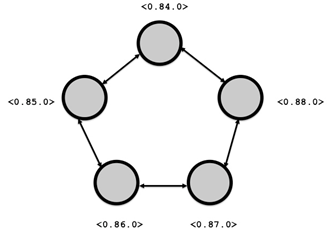
\includegraphics[width=0.8\linewidth]{5_2.png}
    \caption{链接进程的环。注意每个进程在其链接集中有两个其他进程}
    \label{fig:5_2}
\end{figure}

让我们崩溃一个随机进程!我们从 \texttt{pids}列表中随机选择一个 pid 并向它发送 \texttt{:crash}消息:

\begin{code}{}
\begin{minted}[linenos]{elixir}
iex(6) > pids |> Enum.shuffle() |> List.first() |> send(:crash)
:crash
\end{minted}
% \label{lst:id}
\end{code}

现在我们可以检查这些进程是否都没有幸存:

\begin{code}{}
\begin{minted}[linenos]{elixir}
iex(8) > pids |> Enum.map(fn pid -> Process.alive?(pid) end)
[false, false, false, false, false]
\end{minted}
% \label{lst:id}
\end{code}

\subsection{截获退出信号}

到目前为止,我们所做的只是看到链接将所有链接的进程一起带下来。如果我们不希望进程在接收到错误信号时死亡怎么办?我们需要使进程\emph{截获退出信号}。
要使进程截获退出信号,需要调用\texttt{Process.flag(:trap\_exit, true)}。这样做将进程从普通进程转变为系统进程。

普通进程与系统进程有何区别?当系统进程收到错误信号时,它不会像普通进程那样崩溃,而是将信号转换为普通消息,
格式为\mintinline{elixir}|{:EXIT, pid, reason}|,其中\texttt{pid}是被终止的进程,\texttt{reason}是终止的原因。

这样,系统进程可以对被终止的进程采取纠正措施。让我们看看这是如何与两个进程一起工作的,类似于本节中的第一个示例。

首先,我们注意到当前的shell进程:

\begin{code}{}
\begin{minted}[linenos]{elixir}
iex > self
# PID<0.58.0>
\end{minted}
% \label{lst:id}
\end{code}

接下来,通过使其截获退出来将shell进程转变为系统进程:

\begin{code}{}
\begin{minted}[linenos]{elixir}
iex > Process.flag(:trap_exit, true)
false
\end{minted}
% \label{lst:id}
\end{code}

请注意,就像\texttt{Process.link/1}一样,这必须在调用进程内部调用。然后,我们创建一个将要崩溃的进程:

\begin{code}{}
\begin{minted}[linenos]{elixir}
iex > pid =
  spawn(fn ->
    receive do
      :crash -> 1 / 0
    end
  end)

# PID<0.62.0>
\end{minted}
% \label{lst:id}
\end{code}

然后将新创建的进程链接到shell进程:

\begin{code}{}
\begin{minted}[linenos]{elixir}
iex > Process.link(pid)
true
\end{minted}
% \label{lst:id}
\end{code}

现在,如果我们尝试崩溃新创建的进程会发生什么?

\begin{code}{}
\begin{minted}[linenos]{elixir}
iex> send(pid, :crash)
:crash
14:37:10.995 [error] Error in process <0.62.0> with exit value: {badarith,[{erlang,’/‘,[1,0],[]}]}
\end{minted}
% \label{lst:id}
\end{code}

首先,让我们检查shell进程是否存活:

\begin{code}{}
\begin{minted}[linenos]{elixir}
iex > self
# PID<0.58.0>
\end{minted}
% \label{lst:id}
\end{code}

是的!它与之前的进程相同。现在,让我们看看shell进程收到了什么消息:

\begin{code}{}
\begin{minted}[linenos]{elixir}
iex> flush
{:EXIT, #PID<0.62.0>, {:badarith, [{:erlang, :/, [1, 0], []}]}}
\end{minted}
% \label{lst:id}
\end{code}

正如预期的,因为shell进程以\mintinline{elixir}|{:EXIT, pid, reason}|的形式接收到消息。我们稍后在学习如何创建我们自己的监督者进程时会利用这一点。

\subsection{链接已终止/不存在的进程}

让我们尝试链接一个已死的进程,看看会发生什么。首先,我们创建一个很快就退出的进程:

\begin{code}{}\begin{minted}[linenos]{elixir}
iex> pid = spawn(fn -> IO.puts "Bye, cruel world." end)
Bye, cruel world.
#PID<0.80.0>
\end{minted}
% \caption{Listing Caption}
% \label{lst:id}
\end{code}

我们确保这个进程真的死了:

\begin{code}{}
\begin{minted}[linenos]{elixir}
iex > Process.alive?(pid)
false
\end{minted}
% \label{lst:id}
\end{code}

然后我们尝试链接一个已死的进程:

\begin{code}{}
\begin{minted}[linenos]{elixir}
iex> Process.link(pid)
** (ErlangError) erlang error: :noproc:erlang.link(#PID<0.62.0>)
\end{minted}
% \label{lst:id}
\end{code}

\texttt{Process.link/1}确保你正在链接到一个未终止的进程,并且如果你尝试链接到一个已终止或不存在的进程,它会报错。

\subsection{\texttt{spawn\_link/3}:在一个原子步骤中产生和链接}

大多数时候,当生成一个进程时,你会想使用\texttt{spawn\_link/3}。
但它是否只是\texttt{spawn/3}和\texttt{link/1}的简单封装?
换句话说,执行\mintinline{elixir}|spawn_link(Worker, :loop, [])|是否与执行以下操作相同:

\begin{code}{}
\begin{minted}[linenos]{elixir}
pid = spawn(Worker, :loop, [])
Process.link(pid)
\end{minted}
% \label{lst:id}
\end{code}

事实证明,这个故事比这更复杂。\texttt{spawn\_link/3}在一个原子操作中完成生成和链接。为什么这很重要?这是因为当\texttt{link/1}给出一个已终止或不存在的进程时,它会抛出一个错误。由于\texttt{spawn/3}和\texttt{link/1}是两个单独的步骤,\texttt{spawn/3}很可能失败,导致后续调用\texttt{link/1}引发异常。

\subsection{退出消息}

有三种类型的\texttt{:EXIT}消息。你已经看到了第一种,其中返回的终止原因描述了异常。

\subsubsection{正常终止}

进程在正常终止时发送\texttt{:EXIT}消息。这意味着进程没有更多的代码要运行。例如,给出这个进程,其唯一的任务是接收\texttt{:ok}消息然后退出:

\begin{code}{}
\begin{minted}[linenos]{elixir}
iex > pid =
  spawn(fn ->
    receive do
      :ok -> :ok
    end
  end)

# PID<0.73.0>
\end{minted}
% \label{lst:id}
\end{code}

记得链接这个进程:

\begin{code}{}
\begin{minted}[linenos]{elixir}
iex > Process.link(pid)
true
\end{minted}
% \label{lst:id}
\end{code}

然后我们发送\texttt{:ok}消息给这个进程,使其正常退出:

\begin{code}{}
\begin{minted}[linenos]{elixir}
iex > send(pid, :ok)
:ok
\end{minted}
% \label{lst:id}
\end{code}

现在,让我们揭示shell进程收到的消息:

\begin{code}{}
\begin{minted}[linenos]{elixir}
iex> flush
{:EXIT, #PID<0.73.0>, :normal}
\end{minted}
% \label{lst:id}
\end{code}

请注意,对于\emph{正常}链接到刚刚正常退出(即以\texttt{:normal}为原因)的进程的进程,前者进程\emph{不会}被终止。

\subsubsection{强制杀死进程}

进程死亡还有一种方式,那就是使用\texttt{Process.exit(pid, :kill)}。这会向目标进程发送一个\emph{无法截获}的退出信号。这意味着即使进程可能正在截获退出,这也是它无法截获的一个信号。让我们设置shell进程来截获退出:

\begin{code}{}
\begin{minted}[linenos]{elixir}
iex > self
# PID<0.91.0>

iex > Process.flag(:trap_exit, true)
false
\end{minted}
% \label{lst:id}
\end{code}

当我们尝试使用\texttt{:kill}以外的原因使用\texttt{Process.exit/2}杀死它时:

\begin{code}{}
\begin{minted}[linenos]{elixir}
iex> Process.exit(self, :whoops)
true

iex> self
#PID<0.91.0>

iex> flush
{:EXIT, #PID<0.91.0>, :whoops}

iex> self
#PID<0.91.0>
\end{minted}
% \label{lst:id}
\end{code}

在这里,我们已经显示了shell进程已成功截获该信号,因为它在其邮箱中收到了\mintinline{elixir}|{:EXIT, pid, reason}|消息。

现在,让我们尝试\texttt{Process.exit(self, :kill)}:

\begin{code}{}
\begin{minted}[linenos]{elixir}
iex> Process.exit(self, :kill)
** (EXIT from #PID<0.91.0>) killed

iex> self
#PID<0.103.0>
\end{minted}
% \label{lst:id}
\end{code}

这次,请注意shell进程重新启动,进程id不再是我们之前的那个。

\subsection{重新设计环形链}

再次考虑环形链。只有两个进程设置了退出陷阱。我们想创建的是这样的:

\begin{figure}[!ht]
    \centering
    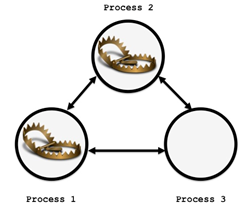
\includegraphics[width=0.8\linewidth]{5_3.png}
    \caption{当进程 2 被终止时会发生什么?}
    \label{fig:5_3}
\end{figure}

再次打开\texttt{lib/ring.ex},添加消息来让进程设置退出陷阱并处理
\mintinline{elixir}|{:EXIT, pid, reason}|:

\begin{code}{ring.ex - 让进程处理 :EXIT 和 :DOWN 消息}
\begin{minted}[linenos]{elixir}
defmodule Ring do
  # …

  def loop do
    receive do
      {:link, link_to} when is_pid(link_to) ->
        Process.link(link_to)
        loop

      :trap_exit ->
        # 1 处理设置退出陷阱的消息
        Process.flag(:trap_exit, true)
        loop

      :crash ->
        1 / 0

      # 2 处理检测 :DOWN 消息
      {:EXIT, pid, reason} ->
        IO.puts("#{inspect(self)} received {:EXIT, #{inspect(pid)}, #{reason}}")
        loop
    end
  end
end
\end{minted}
\label{lst:trap_exit_and_handle_exit_messages}
\end{code}

进程 1 和进程 2 设置了退出陷阱。所有进程彼此链接。现在,当 2 被终止时会发生什么?我们可以创建三个进程来找出答案:

\begin{code}{}
\begin{minted}[linenos]{elixir}
iex> [p1, p2, p3] = Ring.create_processes(3)
[#PID<0.97.0>, #PID<0.98.0>, #PID<0.99.0>]
\end{minted}
% \label{lst:id}
\end{code}

并将它们链接起来:

\begin{code}{}
\begin{minted}[linenos]{elixir}
iex > [p1, p2, p3] |> Ring.link_processes()
\end{minted}
% \label{lst:id}
\end{code}

我们设置前两个进程来设置退出陷阱。

\begin{code}{}
\begin{minted}[linenos]{elixir}
iex > send(p1, :trap_exit)
iex > send(p2, :trap_exit)
\end{minted}
% \label{lst:id}
\end{code}

观察我们终止 \texttt{p2} 时会发生什么:

\begin{code}{}
\begin{minted}[linenos]{elixir}
iex > Process.exit(p2, :kill)

# PID<0.97.0> received {:EXIT, #PID<0.98.0>, killed}#PID<0.97.0> received {:EXIT, #PID<0.99.0>, killed}
\end{minted}
% \label{lst:id}
\end{code}

最后检查,只有 \texttt{p1} 存活:

\begin{code}{}
\begin{minted}[linenos]{elixir}
iex > [p1, p2, p3] |> Enum.map(fn p -> Process.alive?(p) end)
[true, false, false]
\end{minted}
% \label{lst:id}
\end{code}

这里是教训:

如果一个进程设置了退出陷阱,并且它被使用\texttt{Process.exit(pid, :kill)}目标终止,它还是会被终止。
当它死亡时,它会向它的链接集中的进程传播一个\mintinline{elixir}|{:EXIT, \#PID<0.98.0>, :killed}|消息,这\emph{可以}被陷阱捕获。

下面是一个表格,总结所有不同的情况:

\begin{longtable}[]{@{}
  >{\raggedright\arraybackslash}p{(\columnwidth - 4\tabcolsep) * \real{0.3974}}
  >{\raggedright\arraybackslash}p{(\columnwidth - 4\tabcolsep) * \real{0.1795}}
  >{\raggedright\arraybackslash}p{(\columnwidth - 4\tabcolsep) * \real{0.4231}}@{}}
\toprule()
\begin{minipage}[b]{\linewidth}\raggedright
当链接集中的进程\ldots{}
\end{minipage} & \begin{minipage}[b]{\linewidth}\raggedright
设置退出陷阱?
\end{minipage} & \begin{minipage}[b]{\linewidth}\raggedright
那么会发生什么?
\end{minipage} \\
\midrule()
\endhead
正常退出 & 是 & 接收
\mintinline{elixir}|{:EXIT, pid, :normal}| \\
& 否 & 无任何反应 \\
使用 \texttt{Process.exit(pid, :kill)} & 是 & 接收
\mintinline{elixir}|{:EXIT, pid, :normal}| \\
终止 & 否 & 以 \texttt{:killed} 终止 \\
使用 \texttt{Process.exit(pid, other)} & 是 & 接收
\mintinline{elixir}|{:EXIT, pid, other }| \\
终止 & 否 & 以 \texttt{other} 终止 \\
\bottomrule()
\caption{链接集中的进程退出时可能发生的不同情况}
\label{table:5_1}
\end{longtable}

\section{监视器}

有时候,您不需要双向链接。您只是想让一个进程知道另一个进程是否已经宕机,而不影响监视进程本身。
例如,在客户端-服务器架构中,如果客户端由于某种原因宕机,服务器不应该随之宕机。

这就是\emph{监视器}的用途。它们在监视进程和被监视的进程之间建立单向链接。让我们来做一些监视工作!我们创建一个我们最喜欢的可崩溃进程:

\begin{code}{}
\begin{minted}[linenos]{elixir}
iex > pid =
  spawn(fn ->
    receive do
      :crash -> 1 / 0
    end
  end)

# PID<0.60.0>
\end{minted}
% \label{lst:id}
\end{code}

然后,我们告诉shell去监视这个进程:

\begin{code}{}
\begin{minted}[linenos]{elixir}
iex > Process.monitor(pid)
# Reference<0.0.0.80>
\end{minted}
% \label{lst:id}
\end{code}

注意返回值是一个对监视器的\emph{引用}。

引用是独一无二的,可以用来识别消息的来源,尽管这是后面章节的主题。

现在,让进程崩溃并看看会发生什么:

\begin{code}{}
\begin{minted}[linenos]{elixir}
iex> send(pid, :crash)
:crash

iex>
18:55:20.381 [error] Error in process <0.60.0> with exit value: {badarith,[{erlang,’/‘,[1,0],[]}]}`nil
\end{minted}
% \label{lst:id}
\end{code}

让我们检查shell进程的邮箱:

\begin{code}{}
\begin{minted}[linenos]{elixir}
iex> flush
{:DOWN, #Reference<0.0.0.80>, :process, #PID<0.60.0>,{:badarith, [{:erlang, :/, [1, 0], []}]}}
\end{minted}
% \label{lst:id}
\end{code}

注意引用与\texttt{Process.monitor/1}返回的引用相匹配。

\subsection{监视已终止/不存在的进程}

当您尝试监视一个已终止/不存在的进程时会发生什么?继续我们之前的例子,我们首先确信\texttt{pid}确实已经死亡:

\begin{code}{}
\begin{minted}[linenos]{elixir}
iex > Process.alive?(pid)
false
\end{minted}
% \label{lst:id}
\end{code}

然后让我们再次尝试监视:

\begin{code}{}
\begin{minted}[linenos]{elixir}
iex(11) > Process.monitor(pid)
# Reference<0.0.0.114>
\end{minted}
% \label{lst:id}
\end{code}

\texttt{Process.monitor/1}正常处理,不像\texttt{Process.link/1},它会抛出一个\texttt{:noproc}错误。shell进程收到什么消息?

\begin{code}{}
\begin{minted}[linenos]{elixir}
iex(12)> flush
{:DOWN, #Reference<0.0.0.114>, :process, #PID<0.60.0>, :noproc}
\end{minted}
% \label{lst:id}
\end{code}

我们得到一个看起来类似的\texttt{:noproc}消息,不过它不是错误,而是一个平常的消息存在于邮箱中。因此,这个消息可以从邮箱中通过模式匹配得到。

\section{实现一个监督器}

一个监督器是一个负责监视一个或多个进程的进程。被监视的进程可以是工作进程(Worker),甚至是其他监督器。

\begin{figure}[!ht]
    \centering
    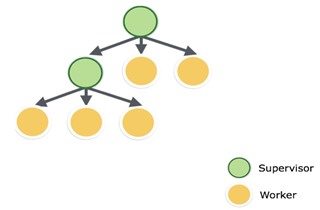
\includegraphics[width=0.8\linewidth]{5_4.png}
    \caption{一个监督树可以与其他监督树层叠。监督器和工作进程都可以被监督}
    \label{fig:5_4}
\end{figure}


监督器和工作进程被安排在一个监督树中。如果任何工作进程死亡,监督器可以重启死掉的工作进程,并且可能根据特定的\emph{重启策略}重启监督树中的其他工作进程。什么是工作进程?它们通常是实现了GenServer,GenFSM或GenEvent行为的进程。

到目前为止,您已经拥有了构建自己的监督器所需的所有构件。一旦您完成了这个部分,监督器将不再显得神奇,尽管这并不意味着它们不再令人敬畏。

\subsection{监督器API}

下表列出了监督器的API以及简要描述:


\begin{longtable}[]{@{}
  >{\raggedright\arraybackslash}p{(\columnwidth - 2\tabcolsep) * \real{0.5000}}
  >{\raggedright\arraybackslash}p{(\columnwidth - 2\tabcolsep) * \real{0.5000}}@{}}
\toprule()
\begin{minipage}[b]{\linewidth}\raggedright
API
\end{minipage} & \begin{minipage}[b]{\linewidth}\raggedright
描述
\end{minipage} \\
\midrule()
\endhead
\texttt{start\_link(child\_spec\_list)} &
给定一个可能为空的子进程规范列表,启动监督器进程和相应的子进程 \\
\texttt{start\_child(supervisor, child\_spec)} &
给定一个监督器pid和一个子进程规范,启动子进程并将其链接到监督器 \\
\texttt{terminate\_child(supervisor, pid)} &
给定一个监督器pid和一个子pid,终止子进程 \\
\texttt{restart\_child(supervisor, pid, child\_spec)} &
给定一个监督器pid、子pid和一个子进程规范,重启子进程并用子进程规范初始化子进程 \\
\texttt{count\_children(supervisor)} &
给定监督器pid,返回子进程的数量 \\
\texttt{which\_children(supervisor)} &
给定监督器pid,返回监督器的状态 \\
\bottomrule()
\caption{我们将实现的API总结}
\label{table:5_2}
\end{longtable}

实现上述API将使我们对实际OTP监督器在底层如何工作有一个非常好的理解。

\subsection{构建我们自己的监督器}

像往常一样,我们从一个新的\texttt{mix}项目开始。由于叫它\texttt{Supervisor}不够原创,而\texttt{MySupervisor}又太无聊,让我们给它一些古英语的风格,称之为\texttt{ThySupervisor}:

\begin{code}{}
\begin{minted}[linenos]{elixir}
% mix new thy_supervisor
\end{minted}
% \label{lst:id}
\end{code}

作为一种复习,我们将使用GenServer行为构建我们的监督器。您可能会惊讶地发现,监督器行为实际上实现了GenServer行为。

\begin{code}{}
\begin{minted}[linenos]{elixir}
defmodule ThySupervisor do
  use GenServer
end
\end{minted}
% \label{lst:id}
\end{code}

\subsection{\texttt{start\_link(child\_spec\_list)}}

首先实现 \texttt{start\_link/1}。

\begin{code}{}
\begin{minted}[linenos]{elixir}
defmodule ThySupervisor do
  use GenServer

  def start_link(child_spec_list) do
    GenServer.start_link(__MODULE__, [child_spec_list])
  end
end
\end{minted}
% \label{lst:id}
\end{code}

这是创建监督进程的主要入口点。在这里,我们调用\texttt{GenServer.start\_link/2},传入模块的名称和包含\texttt{child\_spec\_list}的列表。
\texttt{child\_spec\_list}指定了(可能为空的)\emph{子进程规范}列表。

这是一种告诉监督者它应该管理哪些\emph{类型}的进程的方式。
两个(相似)工作进程的子进程规范可能看起来像这样:\texttt{[\{ThyWorker, :start\_link, []\}, \{ThyWorker, :start\_link, []\}]}。

回想一下,\texttt{GenServer.start\_link/2} 期望实现\texttt{ThySupervisor.init/1}回调。
它将第二个参数(列表)传递给\texttt{:init/1}。让我们来做:


\begin{code}{\texttt{thy\_supervisor.ex} - \texttt{start\_link/1} 和 \texttt{init callback/1}。注意,在\texttt{init/1 callback}中捕获了退出}
\begin{minted}[linenos]{elixir}
defmodule ThySupervisor do
  use GenServer

  #######
  # API #
  #######

  def start_link(child_spec_list) do
    GenServer.start_link(__MODULE__, [child_spec_list])
  end

  ######################
  # 回调函数 #
  ######################

  def init([child_spec_list]) do
    Process.flag(:trap_exit, true)                      #1
    state = child_spec_list
    |> start_children
    |> Enum.into(HashDict.new)

    {:ok, state}
  end
end

#1 让监督进程捕获退出
\end{minted}
\label{lst:start_link_and_init_callback}
\end{code}


我们在这里做的第一件事就是让监督进程捕获退出。这样,它就可以接收来自其子进程的退出信号作为正常消息。

接下来的几行中有很多事情发生。\texttt{child\_spec\_list}被输入到\texttt{start\_children/1}。
很快您将看到,此函数生成子进程并返回一个元组列表。每个元组都是一对,包含新生成子进程的pid 和子进程规范。例如:

\texttt{[\{<0.82.0>, \{ThyWorker, :init, []\}\}, \{<0.84.0>, \{ThyWorker, :init, []\}\}]}

然后这个列表被输入到 \texttt{Enum.into/2}。通过将\texttt{HashDict.new}作为第二个参数传递,我们实际上将元组列表转换为\texttt{HashDict},子进程的 pid 作为键,子进程规范作为值。

\subsubsection{使用 \texttt{Enum.into} 将可枚举类转换为可收集类}

\texttt{Enum.into/2}(和接受额外转换函数的\texttt{Enum.into/3})将一个可枚举(如\texttt{List})插入到一个可收集的对象中(如\texttt{HashDict})。这很有帮助,因为 HashDict知道如果它得到一个元组,第一个元素将成为键,第二个元素将成为值:

\begin{code}{}
\begin{minted}[linenos]{elixir}
iex > h =
  [{:pid1, {:mod1, :fun1, :arg1}}, {:pid2, {:mod2, :fun2, :arg2}}] |> Enum.into(HashDict.new())
\end{minted}
% \label{lst:id}
\end{code}

这将返回一个 HashDict:

\texttt{\#HashDict<[pid2: \{:mod2, :fun2, :arg2\}, pid1: \{:mod1, :fun1, :arg1\}]>}

可以这样检索键:

\begin{code}{}
\begin{minted}[linenos]{elixir}
iex > HashDict.fetch(h, :pid2)
{:ok, {:mod2, :fun2, :arg2}}
\end{minted}
% \label{lst:id}
\end{code}

生成的 \texttt{HashDict} 包含 pid和子进程规范映射,构成了监督进程的\emph{状态},我们以\mintinline{elixir}|{:ok, state}| 元组返回,这是\texttt{init/1} 所期望的。

\subsubsection{\texttt{start\_child(supervisor, child\_spec)}}

我还没有描述在 \texttt{init/1} 中使用的私有函数\texttt{start\_children/1}中发生的事情。让我们稍微跳过一点,先看看\texttt{start\_child/2}。这个函数接收监督者 pid和子进程规范,并将子进程附加到监督者:

\begin{code}{thy\_supervisor.ex - 启动单个子进程}
\begin{minted}[linenos]{elixir}
defmodule ThySupervisor do
  use GenServer

  #######
  # API #
  #######

  def start_child(supervisor, child_spec) do
    GenServer.call(supervisor, {:start_child, child_spec})
  end

  ######################
  # 回调函数 #
  ######################

  def handle_call({:start_child, child_spec}, _from, state) do
    case start_child(child_spec) do
      {:ok, pid} ->
        new_state = state |> HashDict.put(pid, child_spec)
        {:reply, {:ok, pid}, new_state}

      :error ->
        {:reply, {:error, "error starting child"}, state}
    end
  end

  #####################
  # 私有函数 #
  #####################

  defp start_child({mod, fun, args}) do
    case apply(mod, fun, args) do
      pid when is_pid(pid) ->
        Process.link(pid)
        {:ok, pid}

      _ ->
        :error
    end
  end
end
\end{minted}
\label{lst:start_single_child}
\end{code}

\texttt{start\_child/2} API调用向监督者发出同步调用请求。请求包含一个包含\texttt{:start\_child} 原子和子进程规范的元组。
请求由\texttt{handle\_call(\{:start\_child, child\_spec\}, \_, \_)}回调处理。
它尝试使用 \texttt{start\_child/1}私有函数启动一个新的子进程。

成功后,调用进程接收到\mintinline{elixir}|{:ok, pid}|,监督者的状态更新为\texttt{new\_state}。
否则,调用进程接收到带有\texttt{:error} 标签的元组,并提供原因。

\subsubsection{监督者和使用 spawn\_link 生成子进程}

这里有一个重要的点,我们在这里做了一个很大的假设。假设是我们假设创建的进程链接到监督进程。这意味着什么?这意味着我们假设进程是使用
\texttt{spawn\_link} 生成的。事实上,在 OTP监督者行为中假设进程是使用 \texttt{spawn\_link}创建的。

\subsubsection{启动子进程}

现在,我们可以看看 \texttt{start\_children/1}函数,它在 \texttt{init/1} 中使用:

\begin{code}{thy\_supervisor.ex - 启动子进程}
\begin{minted}[linenos]{elixir}
defmodule ThySupervisor do
  # …

  #####################
  # 私有函数 #
  #####################

  defp start_children([child_spec | rest]) do
    case start_child(child_spec) do
      {:ok, pid} ->
        [{pid, child_spec} | start_children(rest)]

      :error ->
        :error
    end
  end

  defp start_children([]), do: []
end
\end{minted}
\label{lst:start_child}
\end{code}

\texttt{start\_children/1}函数接收子进程规范列表,并将子进程规范交给\texttt{start\_child/1},同时累积一个元组列表。
如前所述,每个元组都是一对,包含\texttt{pid} 和子进程规范。

\texttt{start\_child/1}是如何工作的?事实证明,没有太多复杂的机制涉及。
每当我们看到一个\texttt{pid},我们会将其链接到监督进程:

\begin{code}{}
\begin{minted}[linenos]{elixir}
defp start_child({mod, fun, args}) do
  case apply(mod, fun, args) do
    pid when is_pid(pid) ->
      Process.link(pid)
      {:ok, pid}

    _ ->
      :error
  end
end
\end{minted}
% \label{lst:id}
\end{code}

\subsubsection{\texttt{terminate\_child(supervisor, pid)}}

监督器需要一种方法来终止其子进程。以下是API,回调和私有函数的实现:


\begin{code}{ thy\_supervisor.ex -- 终止单个子进程}
\begin{minted}[linenos]{elixir}
defmodule ThySupervisor do
  use GenServer

  #######
  # API #
  #######

  def terminate_child(supervisor, pid) when is_pid(pid) do
    GenServer.call(supervisor, {:terminate_child, pid})
  end

  ######################
  # Callback Functions #
  ######################

  def handle_call({:terminate_child, pid}, _from, state) do
    case terminate_child(pid) do
      :ok ->
        new_state = state |> HashDict.delete(pid)
        {:reply, :ok, new_state}

      :error ->
        {:reply, {:error, "error terminating child"}, state}
    end
  end

  #####################
  # Private Functions #
  #####################

  defp terminate_child(pid) do
    Process.exit(pid, :kill)
    :ok
  end
end
\end{minted}
\label{lst:stop_single_child}
\end{code}

我们使用 \texttt{Process.exit(pid, :kill)}来终止子进程。
还记得我们如何设置监督器来捕获退出吗?当一个子进程被强制杀死使用\texttt{Process.exit(pid, :kill)},监督器将收到一个形式为\mintinline{elixir}|{:EXIT, pid, :killed}|的消息。为了处理这个消息,使用 \texttt{handle\_info/3}回调:

\begin{code}{thy\_supervisor.ex -- :EXIT 消息通过 handle\_info/3 回调处理}
\begin{minted}[linenos]{elixir}
def handle_info({:EXIT, from, :killed}, state) do
  new_state = state |> HashDict.delete(from)
  {:no_reply, new_state}
end
\end{minted}
\label{lst:handle_exit_message}
\end{code}

我们需要做的就是更新监督器状态,通过在\texttt{HashDict}中删除其条目,并在回调中返回适当的元组。

\subsubsection{\texttt{restart\_child(pid, child\_spec)}}

有时手动重启一个子进程是有帮助的。当我们想要重启一个子进程时,我们需要提供进程id和子进程规范。
为什么我们需要将子进程规范与进程id一起传入?原因是你可能想要添加更多的参数,这必须进入子进程规范。

\texttt{restart\_child/2} 私有函数是\texttt{terminate\_child/1} 和\texttt{start\_child/1} 的组合。

\begin{code}{thy\_supervisor.ex -- 重启一个子进程}
\begin{minted}[linenos]{elixir}
defmodule ThySupervisor do
  use GenServer

  #######
  # API #
  #######

  def restart_child(supervisor, pid, child_spec) when is_pid(pid) do
    GenServer.call(supervisor, {:restart_child, pid, child_spec})
  end

  ######################
  # Callback Functions #
  ######################

  def handle_call({:restart_child, old_pid}, _from, state) do
    case HashDict.fetch(state, old_pid) do
      {:ok, child_spec} ->
        case restart_child(old_pid, child_spec) do
          {:ok, {pid, child_spec}} ->
            new_state =
              state
              |> HashDict.delete(old_pid)
              |> HashDict.put(pid, child_spec)

            {:reply, {:ok, pid}, new_state}

          :error ->
            {:reply, {:error, "error restarting child"}, state}
        end

      _ ->
        {:reply, :ok, state}
    end
  end

  #####################
  # Private Functions #
  #####################

  defp restart_child(pid, child_spec) when is_pid(pid) do
    case terminate_child(pid) do
      :ok ->
        case start_child(child_spec) do
          {:ok, new_pid} ->
            {:ok, {new_pid, child_spec}}

          :error ->
            :error
        end

      :error ->
        :error
    end
  end
end
\end{minted}
\label{lst:restart_single_child}
\end{code}

\subsubsection{\texttt{count\_children(supervisor)}}

这个函数返回与监督器链接的子进程的数量。实现很直接:

\begin{code}{thy\_supervisor.ex -- 计算子进程的数量}
\begin{minted}[linenos]{elixir}
defmodule ThySupervisor do
  use GenServer

  #######
  # API #
  #######

  def count_children(supervisor) do
    GenServer.call(supervisor, :count_children)
  end

  ######################
  # Callback Functions #
  ######################

  def handle_call(:count_children, _from, state) do
    {:reply, HashDict.size(state), state}
  end
end
\end{minted}
\label{lst:count_children}
\end{code}

\subsubsection{\texttt{which\_children(supervisor)}}

这与 \texttt{count\_children/1}的实现类似。因为我们的实现很简单,所以完全可以返回整个状态:

\begin{code}{thy\_supervisor.ex -- which\_children/1的简单实现,返回监督器的整个状态}
\begin{minted}[linenos]{elixir}
defmodule ThySupervisor do
  use GenServer

  #######
  # API #
  #######

  def which_children(supervisor) do
    GenServer.call(supervisor, :which_children)
  end

  ######################
  # Callback Functions #
  ######################

  def handle_call(:which_children, _from, state) do
    {:reply, state, state}
  end
end
\end{minted}
\label{lst:which_children_simple}
\end{code}

\subsubsection{\texttt{terminate(reason, state)}}

这个回调被用来关闭监督器进程。在我们终止监督器进程之前,我们需要终止所有与其链接的子进程,这是由\texttt{terminate\_children/1} 私有函数处理的:

\begin{code}{thy\_supervisor.ex -- 终止监督器涉及到首先终止子进程}
\begin{minted}[linenos]{elixir}
defmodule ThySupervisor do
  use GenServer

  ######################
  # Callback Functions #
  ######################

  def terminate(_reason, state) do
    terminate_children(state)
    :ok
  end

  #####################
  # Private Functions #
  #####################

  defp terminate_children([]) do
    :ok
  end

  defp terminate_children(child_specs) do
    child_specs |> Enum.each(fn {pid, _} -> terminate_child(pid) end)
  end

  defp terminate_child(pid) do
    Process.exit(pid, :kill)
    :ok
  end
end
\end{minted}
\label{lst:terminate_supervisor}
\end{code}

 \subsection{ 处理崩溃}

我把最好的留到了最后。当其中一个子进程崩溃时会发生什么?
如果你注意的话,监督器会收到一个看起来像\mintinline{elixir}|{:EXIT, pid, reason}| 的消息。
我们再次使用\texttt{handle\_info/3} 回调来处理退出消息。

有两种情况需要考虑(除了 \texttt{:killed},我们在\texttt{terminate\_child/1} 中处理了)。

第一种情况是进程正常退出。在这种情况下,监督器不需要做任何事情,只需更新其状态:

\begin{code}{thy\_supervisor.ex -- 当一个子进程正常退出时,不做任何操作}
\begin{minted}[linenos]{elixir}
def handle_info({:EXIT, from, :normal}, state) do
  new_state = state |> HashDict.delete(from)
  {:no_reply, new_state}
end
\end{minted}
\label{lst:handle_normal_exit}
\end{code}

第二种情况是进程异常退出并且没有被强制杀死。在这种情况下,监督器应该自动重启失败的进程:

\begin{code}{thy\_supervisor.ex -- 如果一个子进程因为异常原因退出,自动重启它}
\begin{minted}[linenos]{elixir}
def handle_info({:EXIT, old_pid, _reason}, state) do
  case HashDict.fetch(state, old_pid) do
    {:ok, child_spec} ->
      case restart_child(old_pid, child_spec) do
        {:ok, {pid, child_spec}} ->
          new_state =
            state
            |> HashDict.delete(old_pid)
            |> HashDict.put(pid, child_spec)

          {:no_reply, new_state}

        :error ->
          {:no_reply, state}
      end

    _ ->
      {:no_reply, state}
  end
end
\end{minted}
\label{lst:handle_abnormal_exit}
\end{code}

以上的函数并不新鲜。它几乎与 \texttt{restart\_child/2}的实现相同,只是子进程规范是\emph{重用}的。

\subsection{完整的源代码}

以下是我们手动实现的监督器的完整源代码:

\begin{code}{thy\_supervisor.ex 的完整实现}
\begin{minted}[linenos]{elixir}
defmodule ThySupervisor do
  use GenServer

  #######
  # API #
  #######

  def start_link(child_spec_list) do
    GenServer.start_link(__MODULE__, [child_spec_list])
  end

  def start_child(supervisor, child_spec) do
    GenServer.call(supervisor, {:start_child, child_spec})
  end

  def terminate_child(supervisor, pid) when is_pid(pid) do
    GenServer.call(supervisor, {:terminate_child, pid})
  end

  def restart_child(supervisor, pid, child_spec) when is_pid(pid) do
    GenServer.call(supervisor, {:restart_child, pid, child_spec})
  end

  def count_children(supervisor) do
    GenServer.call(supervisor, :count_children)
  end

  def which_children(supervisor) do
    GenServer.call(supervisor, :which_children)
  end

  ######################
  # Callback Functions #
  ######################

  def init([child_spec_list]) do
    Process.flag(:trap_exit, true)

    state =
      child_spec_list
      |> start_children
      |> Enum.into(HashDict.new())

    {:ok, state}
  end

  def handle_call({:start_child, child_spec}, _from, state) do
    case start_child(child_spec) do
      {:ok, pid} ->
        new_state = state |> HashDict.put(pid, child_spec)
        {:reply, {:ok, pid}, new_state}

      :error ->
        {:reply, {:error, "error starting child"}, state}
    end
  end

  def handle_call({:terminate_child, pid}, _from, state) do
    case terminate_child(pid) do
      :ok ->
        new_state = state |> HashDict.delete(pid)
        {:reply, :ok, new_state}

      :error ->
        {:reply, {:error, "error terminating child"}, state}
    end
  end

  def handle_call({:restart_child, old_pid}, _from, state) do
    case HashDict.fetch(state, old_pid) do
      {:ok, child_spec} ->
        case restart_child(old_pid, child_spec) do
          {:ok, {pid, child_spec}} ->
            new_state =
              state
              |> HashDict.delete(old_pid)
              |> HashDict.put(pid, child_spec)

            {:reply, {:ok, pid}, new_state}

          :error ->
            {:reply, {:error, "error restarting child"}, state}
        end

      _ ->
        {:reply, :ok, state}
    end
  end

  def handle_call(:count_children, _from, state) do
    {:reply, HashDict.size(state), state}
  end

  def handle_call(:which_children, _from, state) do
    {:reply, state, state}
  end

  def handle_info({:EXIT, from, :normal}, state) do
    new_state = state |> HashDict.delete(from)
    {:no_reply, new_state}
  end

  def handle_info({:EXIT, from, :killed}, state) do
    new_state = state |> HashDict.delete(from)
    {:no_reply, new_state}
  end

  def handle_info({:EXIT, old_pid, _reason}, state) do
    case HashDict.fetch(state, old_pid) do
      {:ok, child_spec} ->
        case restart_child(old_pid, child_spec) do
          {:ok, {pid, child_spec}} ->
            new_state =
              state
              |> HashDict.delete(old_pid)
              |> HashDict.put(pid, child_spec)

            {:no_reply, new_state}

          :error ->
            {:no_reply, state}
        end

      _ ->
        {:no_reply, state}
    end
  end

  def terminate(_reason, state) do
    terminate_children(state)
    :ok
  end

  #####################
  # Private Functions #
  #####################

  defp start_children([child_spec | rest]) do
    case start_child(child_spec) do
      {:ok, pid} ->
        [{pid, child_spec} | start_children(rest)]

      :error ->
        :error
    end
  end

  defp start_children([]), do: []

  defp start_child({mod, fun, args}) do
    case apply(mod, fun, args) do
      pid when is_pid(pid) ->
        Process.link(pid)
        {:ok, pid}

      _ ->
        :error
    end
  end

  defp terminate_children([]) do
    :ok
  end

  defp terminate_children(child_specs) do
    child_specs |> Enum.each(fn {pid, _} -> terminate_child(pid) end)
  end

  defp terminate_child(pid) do
    Process.exit(pid, :kill)
    :ok
  end

  defp restart_child(pid, child_spec) when is_pid(pid) do
    case terminate_child(pid) do
      :ok ->
        case start_child(child_spec) do
          {:ok, new_pid} ->
            {:ok, {new_pid, child_spec}}

          :error ->
            :error
        end

      :error ->
        :error
    end
  end
end
\end{minted}
\label{lst:thy_supervisor_complete}
\end{code}

\section{一个样例运行(或者:它真的能工作吗?)}

在我们开始测试我们的监督器之前,创建一个新文件\texttt{lib/thy\_worker.ex}:

\begin{code}{lib/thy\_worker.ex -- 一个用于 ThySupervisor 的示例 worker}
\label{lst:thy_worker_for_demo}
\begin{minted}[linenos]{elixir}
defmodule ThyWorker do
  def start_link do
    spawn(fn -> loop end)
  end

  def loop do
    receive do
      :stop ->
        :ok

      msg ->
        IO.inspect(msg)
        loop
    end
  end
end
\end{minted}
\end{code}

我们首先创建一个 worker:
\begin{minted}[linenos]{elixir}
iex > {:ok, sup_pid} = ThySupervisor.start_link([])
  {:ok, #PID<0.86.0>}
\end{minted}


让我们创建一个进程并将其添加到监督器中。我们保存新生成的子进程的 pid。
\begin{minted}[linenos]{elixir}
iex > \{:ok, child_pid\} = ThySupervisor.start\_child(sup\_pid, \{ThyWorker, :start\_link, []\})
\end{minted}

让我们看看监督器中存在哪些链接:
\begin{minted}[linenos]{elixir}
iex(3)> Process.info(sup\_pid, :links)
{:links, [\#PID<0.82.0>, \#PID<0.86.0>]}
\end{minted}

有趣的是,有两个进程链接到了监督器进程。第一个显然是我们刚刚生成的子进程。那么另一个是什么呢?
\begin{minted}[linenos]{elixir}
iex > self
# PID<0.82.0>
\end{minted}

经过一些思考,我们应该能发现,由于监督器进程是由 shell进程生成并链接的,所以它的链接集中会有 shell 的 pid。

让我们杀死子进程:

\mintinline{elixir}|iex > Process.exit(child_pid, :crash)|

当我们再次检查监督器的链接集时会发生什么?

\begin{minted}[linenos]{elixir}
|iex > Process.info(sup_pid, :links)
  {:links, [#PID<0.82.0>, #PID<0.90.0>]}
\end{minted}

太棒了!监督器自动负责生成和链接新的子进程。为了说服我们自己,我们可以查看监督器的状态:

\begin{minted}[linenos]{elixir}
iex > ThySupervisor.which_children(sup_pid)
# HashDict<[{#PID<0.90.0>, {ThyWorker, :start_link, []}}]>
\end{minted}

\section{总结}

在本章中,我们通过几个例子强调了以下几点:

\begin{itemize}

\item  \emph{让它崩溃}的哲学意味着将错误检测和处理委托给另一个进程,而不是过度防御性编程
\item  链接建立了进程之间的双向关系,当其中一个进程发生崩溃时,它们会传播退出信号
\item  监视器在进程之间建立了单向关系,所以当被监视的进程死亡时,监视进程只会收到通知
\item  退出信号可以被所谓的系统进程捕获,这些进程将退出信号转换为普通消息
\item  使用进程和链接实现一个简单的监督器进程
\end{itemize}

在下一章中,我们准备深入研究 OTP Supervisor 行为。我们将学习最重要的Supervisor 特性,并通过构建一个 worker pooler来实验它们。有趣的时刻即将到来!

\chapter{使用监督器实现容错}\label{chapt:fault-tolerent}

本章内容包括:
\begin{enumerate}
\item  如何使用 OTP Supervisor 行为
\item  学习如何使用 ETS,Erlang Term Storage
\item  如何将监督器与普通进程和其他 OTP 行为一起使用
\item  实现一个非常基础的 worker pool 应用
\end{enumerate}

在上一章中,我们使用语言提供的基本元素,即监视器、链接和进程,构建了一个简单的监督器。这应该让你对监督器的内部工作有了很好的理解。

在上一章中我们对你进行了一些挑逗,现在我们终于要使用真正的东西:\emph{OTP
Supervisor 行为}(以下简称为
Supervisor)。监督器的唯一责任是观察和检查一个附加的子进程是否崩溃,并在发生这种情况时采取一些行动。

OTP版本提供了比我们之前的实现更多的功能。例如,\emph{重启策略},它规定了如果出现问题,监督器应该如何重启子进程。
它还提供了在特定时间范围内限制重启次数的选项。这对于防止无限重启特别有用。

要\emph{真正}理解监督器,重要的是要亲自尝试一下。因此,我们将构建这个应用程序(由\emph{Observer}应用程序提供的全部展示):

\begin{figure}[!ht]
    \centering
    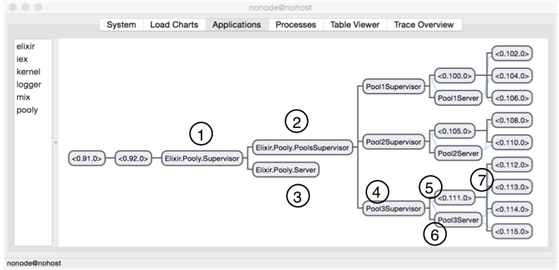
\includegraphics[width=0.8\linewidth]{6_1.png}
    \caption{完成的 worker pool 应用程序}
    \label{fig:6_1}
\end{figure}

图\ref{fig:6_1}显示了完成的 worker pool 应用程序。\#1 是顶级的\texttt{Supervisor}。
它监督 \#2,另一个\texttt{Supervisor}(\texttt{PoolsSupervisor}),
和一个\texttt{GenServer}(\texttt{Pooly.Server}),\#3。
\texttt{PoolsSupervisor}又监督了其他三个\texttt{PoolSupervisor}。
其中一个被标记为\#4。这些监督器都有唯一的名称。
每个\texttt{PoolSupervisor} 又监督了一个 worker supervisor\#5(由其进程 id 表示)和一个 GenServer \#6。
最后,\#7是实际的\texttt{Worker},他们将完成实际的工作。
如果你想知道\texttt{GenServer}是用来做什么的,它们主要是用来为``同一级别''的监督器维护状态。
例如,位于\#6 的 \texttt{GenServer} 帮助监督器 \#5 维护状态。

\section{实现 Pooly -- 一个 Worker Pool 应用}

我们将在两章的过程中构建一个 worker pool。你说什么是 worker
pool?它是管理一池(惊喜!)\texttt{Worker}的东西。你可能需要这个是为了管理对稀缺资源的访问。它可以是任何东西,从
Redis 连接池、web socket 连接池,甚至是 GenServer \texttt{Worker}池。

例如,如果你生成了一百万个进程,每个进程都需要连接到数据库。打开一百万个数据库连接是不切实际的。为了解决这个问题,创建了一个数据库连接池。每次进程需要数据库连接时,它会向池发出请求。一旦进程完成了数据库连接,它就会返回到池中。实际上,资源分配被委托给了
worker pool 应用。

我们将要构建的 worker pool 应用\emph{一点都不}简单。事实上,如果你熟悉
Poolboy,那么很多设计都是为了这个例子而改编的。如果你没有听说过或者没有使用过
Poolboy,也没关系,它不是先决条件。

我相信这是一个非常有益的练习,因为它让你思考那些在简单的例子中不会出现的概念和问题。
你也将亲手使用Supervisor API。

因此,这个例子可能比迄今为止的例子稍微有些挑战性。一些代码/设计可能不是很明显,但主要是因为你没有事后诸葛亮的好处。
但是不用担心,亲爱的读者,因为你将在每一步都得到指导。
我只要求你通过在电脑上输入代码来完成这个代码,然后在下一章的结束时期待启示。

\subsection{计划}

我们将通过四个版本来演进 Pooly 的设计。本章将介绍 Supervisor
的基础知识,并帮助你构建一个非常基础的版本(版本 1)的
Pooly。下一章将完全专注于构建 Pooly 的各种功能。

表\ref{tab:pooly-versions} 列出了 Pooly 的每个版本的特性:

\begin{longtable}[]{@{}ll@{}}
\toprule()
版本 & 特性 \\
\midrule()
\endhead
1 & 支持\emph{单个}池 \\
& 支持\emph{固定}数量的 worker \\
& 当消费者和/或 worker 进程失败时,不进行恢复 \\
2 & 与版本 1 相同 \\
& 当消费者和/或 worker 进程失败时,进行恢复 \\
3 & 支持\emph{多个}池 \\
& 支持\emph{可变}数量的 worker \\
4 & 与版本 3 相同 \\
& 允许 worker 溢出的可变大小的池 \\
& 当所有 worker 都忙时,为消费者进程排队 \\
\bottomrule()
\caption{Pooly 将在四个版本中经历的不同变化}
\label{tab:pooly-versions}
\end{longtable}


为了了解设计将如何演变,版本 1 和版本 2 的样子如下:

\begin{figure}[!ht]
    \centering
    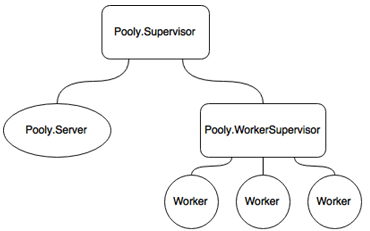
\includegraphics[width=0.8\linewidth]{6_2.png}
    \caption{Pooly 的版本 1 和版本 2}
    \label{fig:6_2}
\end{figure}

矩形代表 \texttt{Supervisor},椭圆代表\texttt{GenServer},圆圈代表 worker 进程。
在版本 3和版本 4 中,设计将如下所示演变:

\begin{figure}[!ht]
    \centering
    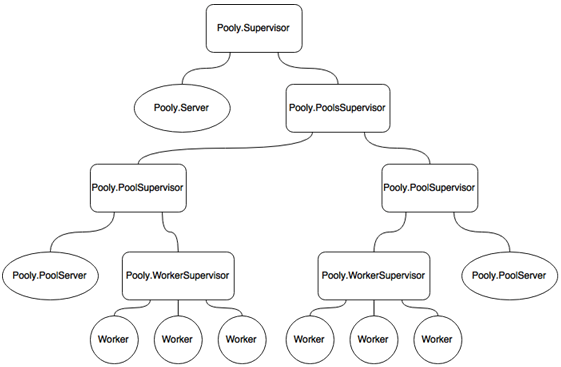
\includegraphics[width=0.8\linewidth]{6_3.png}
    \caption{Pooly 的版本 3 和版本 4}
    \label{fig:6_3}
\end{figure}

从图中,应该很明显为什么它被称为监督\emph{树}。

\subsection{Pooly 的样例运行}

在我们开始实际编码之前,看一下如何使用 Pooly 是很有指导意义的。这将涵盖
Pooly 的第一个版本。


\subsubsection{启动一个池}

为了启动一个池,必须给出一个\emph{池配置}。它提供了 Pooly
初始化池所需的信息。它看起来是这样的:

\begin{code}{}
\begin{minted}[linenos]{elixir}
pool_config = [
  mfa: {SampleWorker, :start_link, []},
  size: 5
]
\end{minted}
% \label{lst:id}
\end{code}

这告诉池创建五个\texttt{SampleWorker}。要启动池:

\begin{code}{}
\begin{minted}[linenos]{elixir}
Pooly.start_pool(pool_config)
\end{minted}
% \label{lst:id}
\end{code}


\subsubsection{检出 Workers}

在 Pooly 的术语中,\emph{检出} workers 意味着从池中请求并获取一个worker。
返回值是一个可用 worker 的 pid。

\begin{code}{}
\begin{minted}[linenos]{elixir}
worker_pid = Pooly.checkout()
\end{minted}
% \label{lst:id}
\end{code}

一旦\emph{消费者进程}获得了一个\texttt{worker\_pid},它可以随意使用它。
如果没有更多的worker 可用会发生什么?
目前,返回\texttt{:noproc}。
我们将在后续版本中提供更复杂的处理方式。


\subsubsection{将 Workers检入回池}

一旦消费者进程完成了 worker 的使用,它必须将其返回到池中,也称为检入worker。
检入 worker 是直接的:

\begin{code}{}
\begin{minted}[linenos]{elixir}
Pooly.checkin(worker_pid)
\end{minted}
% \label{lst:id}
\end{code}


\subsubsection{获取池的状态}

从池中获取一些有用的信息是很有用的。

\begin{code}{}
\begin{minted}[linenos]{elixir}
Pooly.status()
\end{minted}
% \label{lst:id}
\end{code}

目前,这返回一个元组,如\mintinline{elixir}|{3, 2}|。
这意味着有三个空闲的 worker和两个忙碌的 worker。
这就结束了 API 的简短介绍。

\subsection{深入 Pooly,版本 1:奠定基础}

转到你的目录,并使用 \texttt{mix}创建一个新项目:

\begin{code}{}
\begin{minted}[linenos]{elixir}
% mix new pooly
\end{minted}
% \label{lst:id}
\end{code}


\begin{note}{关于源代码的注意事项}
本章的这个项目的不同版本已经分成了不同的分支。
例如,要检出版本3,\texttt{cd} 进入项目文件夹,然后执行\texttt{git checkout version-3}。
\end{note}

\begin{note}{mix 和 --sup 选项}
你可能知道 \texttt{mix} 包含一个叫做\texttt{--sup} 的选项。
这个选项生成一个包含监督树的 OTP应用骨架。
如果省略了这个选项,应用将\emph{没有}监督器和应用回调生成。例如,你可能会想这样创建
Pooly:

\begin{code}{}
\begin{minted}[linenos]{elixir}
% mix new pooly --sup
\end{minted}
% \label{lst:id}
\end{code}

然而,由于我们正在学习,我们将选择无标志版本。
\end{note}

Pooly 的第一个版本只支持一个固定 worker 的单个池。
此外,当消费者或worker 进程失败时,不会进行恢复处理。
在这个版本结束时,Pooly将看起来像这样:

\begin{figure}[!ht]
    \centering
    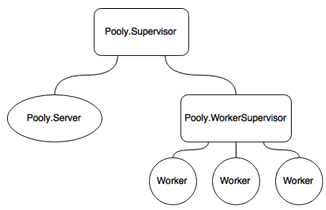
\includegraphics[width=0.8\linewidth]{6_4.png}
    \caption{Pooly 的版本 1}
    \label{fig:6_4}
\end{figure}


如你所见,应用程序由一个顶级监督器(\texttt{Pooly.Supervisor})组成,
它监督两个其他进程,一个GenServer 进程(\texttt{Pooly.Server})和一个 worker监督器(\texttt{Pooly.WorkerSupervisor})。
你可能会记得,从上一章开始,监督器可以自己被监督,因为监督器本身就是进程。

\begin{note}{我该如何开始?}
每当我设计可能有许多监督层次的 Elixir程序时,我总是先画一个草图。这是因为(你很快就会发现)你需要在脑海中保持相当多的东西。
可能比其他语言更多,你必须已经在脑海中有一个粗略的设计,这迫使你稍微提前思考。
\end{note}

当 Pooly 首次启动时,只有 \texttt{Pooly.Server} 附加到\texttt{Pooly.Supervisor}。
当使用池配置启动池时,\texttt{Pooly.Server}首先验证池配置是否有效。

之后,它向 \texttt{Pooly.Supervisor} 发送一个\texttt{:start\_worker\_supervisor}。
这个消息指示\texttt{Pooly.Supervisor} 启动\texttt{Pooly.WorkerSupervisor}。
最后,根据池配置中指定的\texttt{size},告诉\texttt{Pooly.WorkerSupervisor} 启动一定数量的 worker进程。

图\ref{fig:6_2a}说明了 Pooly 版本 1 的工作方式:

\begin{figure}[!ht]
    \centering
    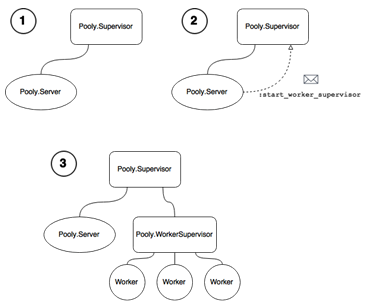
\includegraphics[width=0.8\linewidth]{6_2a.png}
    \caption{Pooly 的各个组件如何初始化}
    \label{fig:6_2a}
\end{figure}

\section{实现 Worker Supervisor}

我们首先将创建一个 worker supervisor。
这个 supervisor将负责监控池中生成的所有 worker。
在 \texttt{lib/pooly}中创建 \texttt{worker\_supervisor.ex}。
就像 GenServer行为(或者说\emph{任何}其他 OTP 行为),这就是如何使用 Supervisor 行为:

\begin{code}{}
\begin{minted}[linenos]{elixir}
defmodule Pooly.WorkerSupervisor do
  use Supervisor
end
\end{minted}
% \label{lst:id}
\end{code}

在代码\ref{lst:worker-supervisor}中,我们定义了老朋友 \texttt{start\_link/1}函数,它作为创建 supervisor 进程的主要入口点。
我们定义的\texttt{start\_link/1} 函数是一个包装函数,它调用\texttt{Supervisor.start\_link/2},并传入模块名和参数。

就像 GenServer 一样,当你定义\texttt{Supervisor.start\_link/2}时,你应该接着实现相应的 \texttt{init/1}回调函数。
传递给 \texttt{Supervisor.start\_link/2}的任何参数都会被传递给 \texttt{init/1} 回调。

\begin{code}{lib/pooly/worker\_supervisor.ex -- 使用模式匹配来验证和解构参数}
\begin{minted}[linenos]{elixir}
defmodule Pooly.WorkerSupervisor do
  use Supervisor

  #######
  # API #
  #######

  # 1
  def start_link({_, _, _} = mfa) do
    Supervisor.start_link(__MODULE__, mfa)
  end

  #############
  # Callbacks #
  #############

  # 2
  def init({m, f, a}) do
    # …
  end
end

# 1 模式匹配参数以确保参数确实是包含三个元素的元组。

# 2 从三元素元组中模式匹配各个元素。
\end{minted}
\label{lst:worker-supervisor}
\end{code}

在 \#1 中,我们声明 \texttt{start\_link}接受一个三元素元组,这将是 worker 进程的模块、函数和参数列表。

注意这里模式匹配的美妙之处。\texttt{\{\_,\_,\_\} = mfa}本质上做了\emph{两件}事。
首先,它断言输入参数必须是一个三元素元组。
其次,输入参数由\texttt{mfa} 引用。
我们可以把它写成\mintinline{elixir}|{m,f,a}|。
然而,由于我们没有使用单个元素,我们使用\texttt{mfa} 传递整个元组。

然后,\texttt{mfa} 被传递给\texttt{init/1}回调。
这次,我们需要使用元组的单个元素,因此在 \#2中我们断言预期的输入参数是\mintinline{elixir}|{m,f,a}|。
\texttt{init/1}回调是实际初始化发生的地方。

\subsection{初始化 Supervisor}

让我们仔细看看 \texttt{init/1} 回调,在 supervisor中,大部分有趣的部分都发生在这里:

\begin{code}{lib/pooly/worker\_supervisor.ex -- 使用子进程和 supervisor规范初始化 supervisor}
\begin{minted}[linenos]{elixir}
defmodule Pooly.WorkerSupervisor do
  #############
  # Callbacks #
  #############

  def init({m, f, a} = x) do
    worker_opts = [restart: :permanent, function: f]

    children = [worker(m, a, worker_opts)]

    opts = [strategy: :simple_one_for_one, max_restarts: 5, max_seconds: 5]

    supervise(children, opts)
  end
end
\end{minted}
\label{lst:worker-supervisor-init}
\end{code}

让我们学习如何解读代码\ref{lst:worker-supervisor-init}。
为了让 supervisor初始化其子进程,你必须给它一个\emph{子进程规范}。
子进程规范(我们在上一章简要介绍过)是supervisor 生成其子进程的配方。

子进程规范是用 \texttt{Supervisor.Spec.worker/3}创建的。
\texttt{Supervisor.Spec} 模块默认被 Supervisor行为导入,所以不需要提供完全限定的版本。

\texttt{init/1}回调的返回值必须是一个\emph{监督器规范}。
为了构造一个监督器规范,我们使用\texttt{Supervisor.Spec.supervise/2} 函数。

\texttt{supervise/2}接受两个参数。
第一个参数是\emph{子列表}。
第二个参数是\emph{选项的关键字列表}。
在上面的代码代码中,这分别由\texttt{children} 和 \texttt{opts}表示。

在我们定义子进程之前,让我们讨论一下\texttt{supervise/2} 的\emph{第二个}参数。

 \subsection{ 监督选项}

我们的示例将 \texttt{supervise/2} 的选项定义如下:

\begin{code}{}
\begin{minted}[linenos]{elixir}
opts = [strategy: :simple_one_for_one, max_restarts: 5, max_seconds: 5]
\end{minted}
% \label{lst:id}
\end{code}

这里可以设置一些选项。最重要的一个是\emph{重启策略},我们接下来会看到。

 \subsection{ 重启策略}

重启策略决定了当出现问题时,监督器如何重启子进程/子进程。为了定义重启策略,需要在重启策略中包含一个
\texttt{strategy} 键。有四种重启策略:

\begin{itemize}

\item
  \texttt{:one\_for\_one}
\item
  \texttt{:rest\_for\_one}
\item
  \texttt{:one\_for\_all}
\item
  \texttt{:simple\_one\_for\_one}
\end{itemize}

让我们快速看一下所有的策略。


\subsubsection{\texorpdfstring{\texttt{:one\_for\_one}}{:one\_for\_one}}

如果该进程死亡,只有该进程会被重启。所有其他进程都不受影响。


\subsubsection{\texorpdfstring{\texttt{:one\_for\_all}}{:one\_for\_all}}

就像三个火枪手一样,如果\emph{任何}进程死亡,监督树下的所有进程都会随之死亡。然后,所有的进程都会再次重启。如果监督树下的所有进程都相互依赖,这种策略就很有用。


\subsubsection{\texorpdfstring{\texttt{:rest\_for\_one}}{:rest\_for\_one}}

如果其中一个进程死亡,那么在该进程之后启动的其他进程都会被终止。然后,死亡的进程和剩余的子进程会被重启。可以把它想象成以圆形方式排列的多米诺骨牌。


\subsubsection{\texorpdfstring{\texttt{:simple\_one\_for\_one}}{:simple\_one\_for\_one}}

前三种策略用于构建静态监督树。这意味着,worker 是通过子进程规范预先指定的。

在 \texttt{:simple\_one\_for\_one}
中,你只需要在子进程规范中指定\emph{一个}条目。从这个监督器生成的每个子进程都会是\emph{同种}类型的进程。

理解 \texttt{:simple\_one\_for\_one}
策略的最好方式就像是一个工厂方法(或者说是 OOP
语言中的构造函数),其中``生产''的 worker
都是相似的。\texttt{:simple\_one\_for\_one}
用于我们想动态创建 worker 的情况。

监督器最初是以空 worker 开始的。然后,worker
动态地附加到监督器上。接下来,我们将看一下允许我们对监督器的行为进行微调的其他选项。


\subsection{最大重启次数和最大秒数}

\texttt{max\_restarts} 和
\texttt{max\_seconds}
转换为监督器在放弃并终止之前可以容忍的最大重启次数和最大秒数。

首先,为什么要有这样的东西呢?主要原因是你不希望你的监督器在真正出现问题时(程序员的错误?)无限制地重启其子进程。因此,你可能希望为监督器放弃的阈值指定一个值。注意,默认情况下,\texttt{max\_restarts}
和 \texttt{max\_seconds} 分别设置为 3 和 5。

在上面的代码代码中,我们指定如果在五秒内有超过五次重启,监督器应该放弃。

 \subsection{ 定义子进程}

现在是时候学习如何定义子进程了。在我们的代码中,子进程是在一个列表中指定的:

\begin{code}{}
\begin{minted}[linenos]{elixir}
children = [worker(m, a, worker_opts)]
\end{minted}
% \label{lst:id}
\end{code}

这告诉我们什么呢?它表示这个监督器有一个子进程,或者在
\texttt{:simple\_one\_for\_one}
重启策略的情况下,有一种\emph{类型}的子进程。(当我们通常不知道在使用
\texttt{:simple\_one\_for\_one} 重启策略时想生成多少个
worker 时,定义多个 worker 是没有意义的。)

\texttt{worker/3}
函数为\emph{worker}创建一个子进程规范,与其兄弟
\texttt{supervisor/3}
相反。这意味着,如果子进程\emph{不是}一个监督器,使用
\texttt{worker/3}。如果你正在监督一个监督器,那么使用
\texttt{supervise/3}。你很快就会使用这两种变体。

这两种变体都接受模块、参数和选项。前两个正如你所期望的那样。第三个参数更有趣。


\subsubsection{子进程规范默认选项}

默认情况下,当你像这样省略选项

\begin{code}{}
\begin{minted}[linenos]{elixir}
children = [worker(m, a)]
\end{minted}
% \label{lst:id}
\end{code}

Elixir 将提供以下选项作为默认值:

\begin{code}{}
\begin{minted}[linenos]{elixir}
[id: module, function: :start_link, restart: :permanent, shutdown: :infinity, modules: [module]]
\end{minted}
% \label{lst:id}
\end{code}


\subsubsection{function:Worker
的启动函数}

\texttt{function} 应该很明显 - 它是
\texttt{mfa} 的
\texttt{f}。有时,worker 的主要入口点是
\texttt{start\_link}
以外的其他函数。这是指定自定义函数要被调用的地方。

restart:重启值

我们将在整个 Pooly 应用中使用两个重启值:

· \texttt{:permanent} - 子进程总是被重启

· \texttt{:temporary} - 子进程永远不会被重启。

在 \texttt{worker\_opts} 中,我们指定了
\texttt{:permanent}。这意味着任何崩溃的 worker
总是会被重启。


\subsubsection{创建一个样例
Worker}

为了测试这个,我们需要一个样例 worker。在
\texttt{lib/pooly} 中创建
\texttt{sample\_worker.ex}。用以下内容填充它:

\begin{code}{lib/pooly/sample\_worker.ex -- 用于测试 Pooly 的 worker}

\begin{minted}[linenos]{elixir}
defmodule SampleWorker do
  use GenServer

  def start_link(_) do
    GenServer.start_link(__MODULE__, :ok, [])
  end

  def stop(pid) do
    GenServer.call(pid, :stop)
  end

  def handle_call(:stop, _from, state) do
    {:stop, :normal, :ok, state}
  end
end
\end{minted}
\label{lst:worker_to_test_supervisor}
\end{code}

\texttt{SampleWorker} 是一个非常简单的GenServer,除了有控制其生命周期的函数外,基本上什么都不做。

\begin{code}{}
\begin{minted}[linenos]{elixir}
iex > {:ok, worker_sup} = Pooly.WorkerSupervisor.start_link({SampleWorker, :start_link, []})
\end{minted}
% \label{lst:id}
\end{code}

现在,我们可以创建一个子进程:

\begin{code}{}
\begin{minted}[linenos]{elixir}
iex > Supervisor.start_child(worker_sup, [[]])
\end{minted}
% \label{lst:id}
\end{code}

返回值是一个看起来像 \mintinline{elixir}|{:ok, \#PID<0.132.0>}|
的两元素元组。向监督器添加更多的子进程。现在,让我们看一下 worker
supervisor 正在监督的所有子进程,使用
\texttt{Supervisor.which\_children/1}:

\begin{code}{}
\begin{minted}[linenos]{elixir}
iex > Supervisor.which_children(worker_sup)
\end{minted}
% \label{lst:id}
\end{code}

结果是一个看起来像这样的列表:

\begin{code}{}
\begin{minted}[linenos]{elixir}
[{:undefined, #PID<0.98.0>, :worker, [SampleWorker]},
{:undefined, #PID<0.101.0>, :worker, [SampleWorker]}]
\end{minted}
% \label{lst:id}
\end{code}

我们也可以计算子进程的数量:

\begin{code}{}
\begin{minted}[linenos]{elixir}
iex > Supervisor.count_children(worker_sup)
\end{minted}
% \label{lst:id}
\end{code}

返回结果应该是不言自明的:

\begin{code}{}
\begin{minted}[linenos]{elixir}
%{active: 2, specs: 1, supervisors: 0, workers: 2}
\end{minted}
% \label{lst:id}
\end{code}

现在来看看监督器的行动!创建另一个子进程,但这次,保存对它的引用:

\begin{code}{}
\begin{minted}[linenos]{elixir}
iex > {:ok, worker_pid} = Supervisor.start_child(worker_sup, [[]])
Supervisor.which_children(worker_sup)
\end{minted}
% \label{lst:id}
\end{code}

应该看起来像这样

\begin{code}{}
\begin{minted}[linenos]{elixir}
[{:undefined, #PID<0.98.0>, :worker, [SampleWorker]},
{:undefined, #PID<0.101.0>, :worker, [SampleWorker]},
{:undefined, #PID<0.103.0>, :worker, [SampleWorker]}]
\end{minted}
% \label{lst:id}
\end{code}

现在,让我们停止刚刚创建的 worker:

\begin{code}{}
\begin{minted}[linenos]{elixir}
iex > SampleWorker.stop(worker_pid)
\end{minted}
% \label{lst:id}
\end{code}

让我们检查一下 worker supervisor 的子进程的状态:

\begin{code}{}
\begin{minted}[linenos]{elixir}
iex(8)> Supervisor.which_children(worker_sup)
[{:undefined, #PID<0.98.0>, :worker, [SampleWorker]},
{:undefined, #PID<0.101.0>, :worker, [SampleWorker]},
{:undefined, #PID<0.107.0>, :worker, [SampleWorker]}]
\end{minted}
% \label{lst:id}
\end{code}

哇哦!监督器自动重启了停止的
worker!每当监督器自动重启失败的子进程时,我仍然会有一种温暖的感觉。在其他语言中获得类似的东西通常需要更多的工作。接下来,我们将看一下如何实现
\texttt{Pooly.Server}。

\section{实现服务器:操作的大脑}

现在,我们将处理操作的大脑。一般来说,你希望让监督器尽可能少的逻辑,因为代码越少,出错的可能性就越小。

因此,我们引入了一个 GenServer
进程,它将处理应用程序的大部分有趣的逻辑。服务器进程必须与顶级监督器和
worker 监督器进行通信。一种方法是使用\emph{命名进程}:

\begin{figure}[!ht]
    \centering
    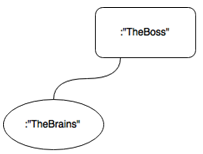
\includegraphics[width=0.8\linewidth]{6_3a.png}
    \caption{命名进程允许其他进程通过它们的名称引用它们}
    \label{fig:6_3a}
\end{figure}


在这种情况下,两个进程可以通过各自的名称相互引用。然而,更一般的解决方案是让服务器进程将对顶级监督器和worker 监督器的引用作为其\emph{状态}的一部分。

服务器将从哪里获得对两个监督器的引用呢?当顶级监督器启动服务器时,监督器可以将其自己的
pid 传递给服务器。事实上,这正是我们在实现顶级监督器时要做的事情。

\begin{figure}[!ht]
    \centering
    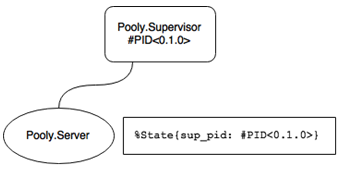
\includegraphics[width=0.8\linewidth]{6_3b.png}
    \caption{监督器的引用存储在 Pooly.Server 的状态中}
    \label{fig:6_3b}
\end{figure}


现在,由于服务器有了对顶级监督器的引用,它可以告诉它使用
\texttt{Pooly.WorkerSupervisor}
模块启动一个子进程,传入池配置的相关部分,然后
\texttt{Pooly.WorkerSupervisor} 将处理剩下的部分。

服务器进程还维护着池的状态。我们已经知道,服务器必须存储对顶级监督器和
worker
监督器的引用。它还应该存储什么呢?首先,它需要存储关于池的详细信息,比如要创建什么样的
worker,以及要创建多少个。池配置提供了这些信息。

 \subsection{ 池配置}

服务器接受一个以关键字列表形式的池配置。在这个版本中,一个示例池配置可能是这样的:

\begin{code}{}
\begin{minted}[linenos]{elixir}
[mfa: {SampleWorker, :start_link, []}, size: 5]
\end{minted}
% \label{lst:id}
\end{code}

键 \texttt{mfa} 代表要创建的 worker 池的
\texttt{m}odule(模块)、\texttt{f}unction(函数)和
\texttt{a}rguments(参数)列表。\texttt{size}
是要创建的 worker 进程的数量。

说了这么多,让我们看一些代码!创建一个名为\texttt{server.ex} 的文件,并将其放在\texttt{lib/pooly} 中。

目前,我们将使 \texttt{Pooly.Server}成为一个\emph{命名进程},
这意味着我们可以使用模块名(即\texttt{Pooly.Server.status} 而不是\texttt{Pool.Server.status(pid)})引用服务器进程。
代码\ref{lst:server-start-link} 展示了如何做到这一点:


\begin{code}{lib/pooly/server.ex --将对顶级监督器和池配置的引用传递给初始化服务器进程}

\begin{minted}[linenos]{elixir}
defmodule Pooly.Server do
  use GenServer
  import Supervisor.Spec

  #######
  # API #
  #######

  def start_link(sup, pool_config) do
    GenServer.start_link(__MODULE__, [sup, pool_config], name: __MODULE__)
  end
end
\end{minted}
\label{lst:server-start-link}
\end{code}

服务器进程需要对顶级监督器进程和池配置的引用,我们将其作为\texttt{[sup, pool\_config]} 传入。

现在,我们需要实现 \texttt{init/1}回调。
\texttt{init/1}回调有两个职责。
第一个是验证池配置。第二个是初始化状态,就像所有好的\texttt{init} 回调一样。

 \subsection{ 验证池配置}

有效的池配置看起来像这样:

\begin{code}{}
\begin{minted}[linenos]{elixir}
[mfa: {SampleWorker, :start_link, []}, size: 5]
\end{minted}
% \label{lst:id}
\end{code}

这是一个带有两个键 \texttt{mfa} 和\texttt{size}的关键字列表。任何其他键都将被忽略。
当函数遍历池配置关键字列表时,状态会逐渐建立起来:

\begin{code}{lib/pooly/server.ex -- 使用多个 init/2 函数子句设置服务器的状态}

\begin{minted}[linenos]{elixir}
defmodule Pooly.Server do
  use GenServer

  # 1
  defmodule State do
    defstruct sup: nil, size: nil, mfa: nil
  end

  #############
  # Callbacks #
  #############

  # 2
  def init([sup, pool_config]) when is_pid(sup) do
    init(pool_config, %State{sup: sup})
  end

  # 3
  def init([{:mfa, mfa} | rest], state) do
    init(rest, %{state | mfa: mfa})
  end

  # 4
  def init([{:size, size} | rest], state) do
    init(rest, %{state | size: size})
  end

  # 5
  def init([_ | rest], state) do
    init(rest, state)
  end

  # 6
  def init([], state) do
    # 7
    send(self, :start_worker_supervisor)
    {:ok, state}
  end
end
\end{minted}
% \label{lst:id}
\end{code}

代码 6.5 设置了服务器的状态。\#1 声明了一个
\texttt{struct},它作为服务器状态的容器。\#2 是当
\texttt{GenServer.start\_link/3} 被调用时的回调。

\texttt{init/1} 回调接收顶级监督器的 pid
和池配置。然后它调用
\texttt{init/2},它接收池配置和包含顶级监督器 pid
的新状态。

关键字列表中的每个元素都由一个两元素元组表示,其中第一个元素是键,第二个元素是值。

目前,我们对记住池配置的 \texttt{mfa} 和
\texttt{size} 值感兴趣。\#3 和 \#4
正是这样做的。如果我们想向状态添加更多字段,我们只需要添加更多具有适当模式的函数子句。\#5
忽略了我们不关心的任何选项。

最后,一旦我们像 \#6
那样遍历了整个列表,我们期望状态已经被初始化。记住,\texttt{init/1}
的有效返回值之一是 \mintinline{elixir}|{:ok, state}|。由于
\texttt{init/1} 调用
\texttt{init/2},并且在 \#6
中的空列表情况将是最后被调用的函数子句,因此它应该返回
\mintinline{elixir}|{:ok, state}|。

\#7 上的那行奇怪的代码是什么呢?一旦我们到达
\#6,我们就确信状态已经建立。这时我们可以启动我们之前实现的 worker
supervisor。发生的事情是,服务器进程向自己发送了一条消息。因为
\texttt{send/2} 立即返回,所以
\texttt{init/1} 回调不会被阻塞。你不希望
\texttt{init/1} 超时,对吧?

虽然 \texttt{init/1}
函数的数量可能看起来有些多,但不用担心。单独来看,每个函数都尽可能小。如果没有在函数参数中进行模式匹配,我们需要编写一个大的条件语句来捕获所有的可能性。


\subsection{启动 WorkerSupervisor}

当服务器进程使用 \texttt{send/2}向自己发送消息时,该消息将使用 \texttt{handle\_info/2}进行处理:

\begin{code}{lib/pooly/server.ex -- 启动 worker supervisor 的回调处理器}

\begin{minted}[linenos]{elixir}
defmodule Pooly.Server do
  defstruct sup: nil, worker_sup: nil, size: nil, workers: nil, mfa: nil

  #############
  # Callbacks #
  #############

  def handle_info(:start_worker_supervisor, state = %{sup: sup, mfa: mfa, size: size}) do
    # 1
    {:ok, worker_sup} = Supervisor.start_child(sup, supervisor_spec(mfa))
    # 2
    workers = prepopulate(size, worker_sup)
    # 3
    {:noreply, %{state | worker_sup: worker_sup, workers: workers}}
  end

  #####################
  # Private Functions #
  #####################

  defp supervisor_spec(mfa) do
    opts = [restart: :temporary]
    # 4
    supervisor(Pooly.WorkerSupervisor, [mfa], opts)
  end
end
\end{minted}
% \label{lst:id}
\end{code}

代码 6.6 中有很多事情正在进行。由于服务器进程的状态包含顶级监督器 pid(\texttt{sup}),我们使用监督器 pid 和监督器规范调用\texttt{Supervisor.start\_child/2}。
之后,我们传递新创建的worker 监督器 pid(\texttt{worker\_sup}),并使用它来启动\texttt{size} 数量的 worker。
最后,我们用 worker 监督器pid 和新创建的 worker 更新状态。

\#1 返回一个元组,其中 worker 监督器 pid 作为第二个元素。
在 \#4中,监督器规范由一个 worker监督器作为子进程组成。
注意,我们使用监督器变体,而不是

\begin{code}{}
\begin{minted}[linenos]{elixir}
worker(Pooly.WorkerSupervisor, [mfa], opts)
\end{minted}
% \label{lst:id}
\end{code}

我们使用监督器变体:

\begin{code}{}
\begin{minted}[linenos]{elixir}
supervisor(Pooly.WorkerSupervisor, [mfa], opts)
\end{minted}
% \label{lst:id}
\end{code}

这里,我们在 \#4 中作为监督器规范传入
\texttt{restart: :temporary}。这意味着顶级监督器不会自动重启
worker
监督器。这似乎有点奇怪。为什么呢?原因是我们想做的不仅仅是让监督器重启子进程。因为我们想要一些自定义的恢复规则,我们用
\texttt{restart: :temporary}
``关闭''了监督器自动重启失败的 worker 的默认行为。

请注意,这个版本并没有处理任何 worker
应该发生崩溃时的恢复。后续的版本将修复这个问题。接下来让我们处理 worker
的预填充。


\subsection{预填充 Worker Supervisor 的Worker}

给定池配置中的 \texttt{size} 选项,worker
监督器可以预填充自己的一组 worker。代码 6.7 中的
\texttt{prepopulate/2} 函数接收一个大小和 worker 监督器
pid,并构建一个 \texttt{size} 数量的 worker 列表,如
\#1 所示:

\begin{code}{lib/pooly/server.ex -- 预填充 worker supervisor 的 worker}

\begin{minted}[linenos]{elixir}
defmodule Pooly.Server do
  #####################
  # Private Functions #
  #####################

  defp prepopulate(size, sup) do
    prepopulate(size, sup, [])
  end

  defp prepopulate(size, _sup, workers) when size < 1 do
    workers
  end

  defp prepopulate(size, sup, workers) do
    # 1
    prepopulate(size - 1, sup, [new_worker(sup) | workers])
  end

  defp new_worker(sup) do
    # 2
    {:ok, worker} = Supervisor.start_child(sup, [[]])
    worker
  end
end

# 1 创建了一个附加到 worker 监督器的 worker 列表。 
# 2 动态创建一个worker 进程并将其附加到监督器。
\end{minted}
% \label{lst:id}
\end{code}




\subsection{创建新的 Worker进程}

代码 6.7 中的 \texttt{new\_worker/1}
函数值得一看。在这里,我们再次使用
\texttt{Supervisor.start\_child/2} 来生成 worker
进程。我们传入的是一个\emph{参数列表},而不是一个子进程规范。

Supervisor.start\_child/2 的两种形式

\texttt{Supervisor.start\\\_child/2}
有两种形式。第一种接受一个子进程规范:

\begin{code}{}
\begin{minted}[linenos]{elixir}
{:ok, sup} = Supervisor.start\_child(sup, supervisor\_spec(mfa))
\end{minted}
% \label{lst:id}
\end{code}

另一种形式接受一个参数列表:

\begin{code}{}
\begin{minted}[linenos]{elixir}
{:ok, worker} = Supervisor.start\_child(sup, [[]])
\end{minted}
% \label{lst:id}
\end{code}

你应该使用哪种形式呢?\texttt{Pooly.WorkerSupervisor}
使用的是 \texttt{:simple\\\_one\\\_for\\\_one}
重启策略。这意味着子进程规范已经被预定义了。这意味着第一种形式是不行的 -
你需要的是第二种形式。

第二种版本允许你向 worker 传递\emph{额外}的参数。在底层,当创建
\texttt{Pooly.WorkerSupervisor}
时在子进程规范中定义的参数会与传入
\texttt{Supevisor.start\\\_child/2}
的列表\emph{连接},然后结果会在初始化期间传递给 worker 进程。

\texttt{new\_worker/2} 的返回结果是新创建的 worker 的
pid。我们还没有实现从池中\emph{取出} worker,以及其对应的\emph{将 worker
放回}池中的方法。这两个操作也被分别称为\emph{取出}和\emph{归还}
worker。但在我们做这个之前,我们需要稍作改道,讨论一下下一节的 ETS。


\subsection{ETS初探}

在本章和下一章中,我们将使用 ETS,也称为 Erlang Term Storage。
本节将为你提供足够的背景知识,以理解本章和下一章中的 ETS相关代码。


\subsubsection{什么是 ETS}

它本质上是一个非常高效的内存数据库,专门用于存储 Erlang/Elixir
数据。它能够存储大量的数据而不会出现问题。数据访问也是在常数时间内完成的。它是
Erlang 的免费功能,这意味着我们必须使用 \texttt{:ets}
从 Elixir 中访问它。


\subsubsection{创建新的 ETS 表}

使用 \texttt{:ets.new/2}
创建表。让我们创建一个表来存储我妈妈最喜欢的艺术家,他们的出生日期和流派:

\begin{code}{}
\begin{minted}[linenos]{elixir}
iex > :ets.new(:mum_faves, [])
12308
\end{minted}
% \label{lst:id}
\end{code}

最基本的形式接受一个表示表名的原子和一个空的选项列表。\texttt{:ets.new/2}
的返回值是一个表 ID,类似于 pid。创建 ETS
表的进程被视为\emph{所有者进程}。在这种情况下,\texttt{iex}
进程是所有者。最常见的选项与 ETS
表的\emph{类型}、\emph{访问权限}以及是否\emph{命名}有关。


\subsubsection{ETS 表类型}

ETS 表有四种不同的形式:

\begin{itemize}

\item  \texttt{:set}

  \begin{itemize}
  
  \item
    这是默认的。它的特性与你在 CS101
    中可能学过的集合数据结构完全相同(无序,每个唯一键映射到一个元素)。
  \end{itemize}
\item  \texttt{:ordered\_set}

  \begin{itemize}
  
  \item    \texttt{:set} 的排序版本。
  \end{itemize}
\item  \texttt{:bag}

  \begin{itemize}
  
  \item    允许具有相同键的行,但行必须不同。
  \end{itemize}
\item  \texttt{:duplicate\_bag}

  \begin{itemize}
  
  \item    与 \texttt{:bag} 相同,但没有行唯一性的限制。
  \end{itemize}
\end{itemize}

在本章和下一章中,我们将使用\texttt{:set},这本质上意味着我们不需要在选项列表中指定表类型。
如果我们想要具体化,我们会这样创建表:

\begin{code}{}
\begin{minted}[linenos]{elixir}
iex > :ets.new(:mum_faves, [:set])
\end{minted}
% \label{lst:id}
\end{code}


\subsubsection{访问权限}

访问权限控制哪个进程可以从 ETS 表中读取和写入。有三个选项:

\begin{itemize}

\item  \texttt{:protected} -  所有者进程具有完全的读写权限。所有其他进程只能从中读取。这是默认设置。
\item  \texttt{:public} - 对读写没有限制。
\item  \texttt{:private} -  只有所有者进程可以从表中读取和写入。
\end{itemize}

在本章中,我们将使用 \texttt{:private}表,因为我们将存储其他池无权知道的与池相关的数据。
所以,假设我的妈妈对她的折衷音乐品味非常害羞,想要将表设为私有:

\begin{code}{}\begin{minted}[linenos]{elixir}
iex > :ets.new(:mum_faves, [:set, :private])
\end{minted}
% \label{lst:id}
\end{code}


\subsubsection{命名表}

注意,当我们创建 ETS
表时,我们提供了一个原子。这有些误导,因为我们\emph{不能}在不提供\texttt{:named\_table} 选项的情况下使用\texttt{:mum\_faves} 来引用表。
因此,要使用\texttt{:mum\_faves} 而不是像\texttt{12308} 这样的无法理解的引用,你可以这样做:

\begin{code}{}\begin{minted}[linenos]{elixir}
iex > :ets.new(:mum_faves, [:set, :private, :named_table])
\end{minted}
% \label{lst:id}
\end{code}

\texttt{:mum\_faves}
注意,如果你再次尝试运行上面的行,你会得到:

\begin{code}{}\begin{minted}[linenos]{elixir}
iex> :ets.new(:mum_faves, [:set, :private, :named_table])
** (ArgumentError) argument error
(stdlib) :ets.new(:mum_faves, [:set, :private, :named_table])
\end{minted}
% \label{lst:id}
\end{code}

这是因为名称应该是 ETS 表的\emph{唯一}引用。


\subsubsection{插入和删除数据}

使用 \texttt{:ets.insert/2}函数插入数据。
第一个参数是表标识符(数字或名称),第二个参数是数据。
数据以元组的形式出现,其中第一个元素是键,第二个可以是\emph{任何}、\emph{任意嵌套}的项。
这里有一些我妈妈的最爱:

\begin{code}{}\begin{minted}[linenos]{elixir}
iex > :ets.insert(:mum_faves, {"Michael Bolton", 1953, "Pop"})
true
iex > :ets.insert(:mum_faves, {"Engelbert Humperdinck", 1936, "Easy Listening"})
true
iex > :ets.insert(:mum_faves, {"Justin Beiber", 1994, "Teen"})
true
iex > :ets.insert(:mum_faves, {"Jim Reeves", 1923, "Country"})
true
iex > :ets.insert(:mum_faves, {"Cyndi Lauper", 1953, "Pop"})
true
\end{minted}
% \label{lst:id}
\end{code}

我们可以使用 \texttt{:ets.tab2list/1} 查看表中的内容:

\begin{code}{}\begin{minted}[linenos]{elixir}
iex > :ets.tab2list(:mum_faves)

[
  {"Michael Bolton", 1953, "Pop"},
  {"Cyndi Lauper", 1953, "Pop"},
  {"Justin Beiber", 1994, "Teen"},
  {"Engelbert Humperdinck", 1936, "Easy Listening"},
  {"Jim Reeves", 1923, "Country"}
]
\end{minted}
% \label{lst:id}
\end{code}

注意返回结果是一个列表,列表中的元素是无序的。好吧,我撒谎了。
我的妈妈其实并不是Justin Beiber的粉丝\pagenote{她也不是Cyndi Lauper 的粉丝,但我在写这篇文章的时候正在听 ``Girls just want to have fun''。}。
让我们纠正这一点:

\begin{code}{}\begin{minted}[linenos]{elixir}
iex > :ets.delete(:mum_faves, "Justin Beiber")
true
\end{minted}
% \label{lst:id}
\end{code}


\subsubsection{查找数据}
如果我们不能检索数据,那么表就没有用。最简单的方法是使用键。迈克尔·博尔顿的出生年份是什么?让我们找出来:

\begin{code}{}\begin{minted}[linenos]{elixir}
iex > :ets.lookup(:mum_faves, "Michael Bolton")
[{"Michael Bolton", 1953, "Pop"}]
\end{minted}
% \label{lst:id}
\end{code}

为什么结果是一个列表?回想一下,ETS 支持其他类型,比如\texttt{:duplicate\_bag},它允许重复的行。
因此,表示这个的最通用的数据结构就是简单的列表。

如果你想按\emph{年份}进行搜索怎么办?我们可以使用\texttt{:ets.match/2}:

\begin{code}{}\begin{minted}[linenos]{elixir}
iex > :ets.match(:mum_faves, {:"$1", 1953, :"$2"})
[["Michael Bolton", "Pop"], ["Cyndi Lauper", "Pop"]]
\end{minted}
% \label{lst:id}
\end{code}

我们传入一个\emph{模式},乍一看可能有点奇怪。
由于我们只是使用年份进行查询,我们使用\texttt{\$N} 作为占位符,其中\texttt{N}是一个整数。
这些数字对应于每个匹配结果中元素的顺序。让我们交换占位符:

\begin{code}{}
\begin{minted}[linenos]{elixir}
iex(20) > :ets.match(:mum_faves, {:"$2", 1953, :"$1"})
[["Pop", "Michael Bolton"], ["Pop", "Cyndi Lauper"]]
\end{minted}
% \label{lst:id}
\end{code}

你现在可以清楚地看到,流派在艺术家名字之前。如果你只关心返回艺术家呢?我们可以使用下划线来省略流派,就像这样:

\begin{code}{}
\begin{minted}[linenos]{elixir}
iex(25) > :ets.match(:mum_faves, {:"$1", 1953, :_})
[["Michael Bolton"], ["Cyndi Lauper"]]
\end{minted}
% \label{lst:id}
\end{code}

关于 ETS 还有更多的知识要学,但这就是你需要理解代码中 ETS部分的所有信息。
让我们回到从池中取出 worker 的问题。

 \subsection{ 检出 Worker}

当消费者进程从池中检出一个 worker时,有一些关键的物流问题需要处理,比如:

\begin{itemize}

\item  消费者进程的 pid 是什么?
\item  消费者进程正在使用哪个 worker pid?
\end{itemize}

服务器需要\emph{监控}消费者进程,因为如果它死掉,服务器进程需要知道并采取恢复行动。再次强调,我们还没有实现恢复代码,但正在打下基础。

我们还需要知道消费者进程使用的是哪个worker,这样我们就可以确定哪个消费者进程使用了哪个 workerpid。下面是检出 worker 的实现:

\begin{code}{lib/pooly/server.ex -- 检出 worker}

\begin{minted}[linenos]{elixir}
defmodule Pooly.Server do
  #######
  # API #
  #######

  def checkout do
    GenServer.call(__MODULE__, :checkout)
  end

  #############
  # Callbacks #
  #############

  # 1
  def handle_call(:checkout, {from_pid, _ref}, %{workers: workers, monitors: monitors} = state) do
    # 2
    case workers do
      [worker | rest] ->
        # 3
        ref = Process.monitor(from_pid)
        # 4
        true = :ets.insert(monitors, {worker, ref})
        {:reply, worker, %{state | workers: rest}}

      [] ->
        {:reply, :noproc, state}
    end
  end
end
\end{minted}
% \label{lst:id}
\end{code}

我们将使用 ETS表来存储监视器。
回调函数的实现很有趣。有两种情况需要处理。
要么我们还有剩余的worker 可以检出,要么我们没有。
在后一种情况下,我们返回\mintinline{elixir}|{:reply, :noproc, state}|,表示没有可用的进程。
在大多数关于GenServers 的例子中,你会看到 \texttt{from}参数通常被忽略:

\begin{code}{}
\begin{minted}[linenos]{elixir}
def handle_call(:checkout, _from, state) do
  # …
end
\end{minted}
% \label{lst:id}
\end{code}

在这种情况下,\texttt{from}是\emph{非常}有用的。
注意,\texttt{from}实际上是一个由客户端 pid 和标签(引用)组成的两元素元组。
在 \#1中,我们只关心客户端的 pid。
我们使用客户端的 pid(\texttt{from\_pid}) 并让服务器进程监控它。
然后在 \#4中我们使用生成的引用并将其添加到 ETS 表中。
最后,状态更新为少一个worker。

现在我们需要更新 \texttt{init/1}回调,因为我们引入了一个新的 \texttt{monitors}字段来存储监视器 ETS 表:
\begin{code}{lib/pooly/server.ex -- 将监视器 ETS表的引用存储到服务器的状态中}
\begin{minted}[linenos]{elixir}
defmodule Pooly.Server do
  #############
  # Callbacks #
  #############

  def init([sup, pool_config]) when is_pid(sup) do
    # 1
    monitors = :ets.new(:monitors, [:private])
    # 1
    init(pool_config, %State{sup: sup, monitors: monitors})
  end
end

# 1 更新状态以存储监视器表
\end{minted}
% \label{lst:id}
\end{code}



 \subsection{ 检入 Worker}

检出 worker 的反向操作是(等待)检入。事实上,代码 6.10 中的实现与代码是相反的:
\begin{code}{lib/pooly/server.ex -- 检入 worker}

\begin{minted}[linenos]{elixir}
defmodule Pooly.Server do
  #######
  # API #
  #######

  def checkin(worker_pid) do
    GenServer.cast(__MODULE__, {:checkin, worker_pid})
  end

  #############
  # Callbacks #
  #############

  def handle_cast({:checkin, worker}, %{workers: workers, monitors: monitors} = state) do
    case :ets.lookup(monitors, worker) do
      [{pid, ref}] ->
        true = Process.demonitor(ref)
        true = :ets.delete(monitors, pid)
        {:no_reply, %{state | workers: [pid | workers]}}

      [] ->
        {:no_reply, state}
    end
  end
end
\end{minted}
% \label{lst:id}
\end{code}

给定一个 worker pid (\texttt{worker}),在
\texttt{monitors} ETS
表中搜索条目。如果没有找到条目,什么也不做。如果找到了条目,那么消费者进程将被取消监控,从
ETS 表中删除条目,并用 worker 的 pid 更新服务器状态的
\texttt{workers} 字段。


\subsection{获取池的状态}

我们希望对我们的池有一些了解。这是很容易实现的:

\begin{code}{lib/pooly/server.ex -- 获取池的状态}

\begin{minted}[linenos]{elixir}
defmodule Pooly.Server do
  #######
  # API #
  #######

  def status do
    GenServer.call(__MODULE__, :status)
  end

  #############
  # Callbacks #
  #############

  def handle_call(:status, _from, %{workers: workers, monitors: monitors} = state) do
    {:reply, {length(workers), :ets.info(monitors, :size)}, state}
  end
end
\end{minted}
% \label{lst:id}
\end{code}

这提供了一些关于可用 worker 的数量和已检出(忙碌)worker 的数量的信息。

\section{实现顶级监督器}

在我们可以宣布版本 1 功能完整之前,还有最后一部分。在
\texttt{lib/pooly} 中创建
\texttt{supervisor.ex}。这将是顶级监督器。下面是完整的实现:

\begin{code}{lib/pooly/supervisor.ex -- 顶级监督器}

\begin{minted}[linenos]{elixir}
defmodule Pooly.Supervisor do
  use Supervisor

  def start_link(pool_config) do
    Supervisor.start_link(__MODULE__, pool_config)
  end

  def init(pool_config) do
    children = [
      worker(Pooly.Server, [self, pool_config])
    ]

    opts = [strategy: :one_for_all]

    supervise(children, opts)
  end
end
\end{minted}
% \label{lst:id}
\end{code}

你可以看到,\texttt{Pooly.Supervisor} 的结构与
\texttt{Pooly.WorkerSupervisor}
非常相似。\texttt{start\_link/1} 函数接受一个
\texttt{pool\_config}。\texttt{init/1}
回调接收池配置。

\texttt{children} 列表由
\texttt{Pooly.Server}
组成。回想一下,\texttt{Pooly.Server.start\_link/2}
接受两个参数,首先是顶级监督器进程的 pid(我们现在正在处理的)和池配置。

那么 worker
监督器呢?为什么我们不监督它?现在应该很清楚,因为是\emph{服务器}启动了
worker 监督器,所以一开始它并没有被包含在这里。

我们在这里使用的重启策略是
\texttt{:one\_for\_all}。为什么不说,\texttt{:one\_for\_one}?想一想。

当服务器崩溃时会发生什么?它会丢失所有的状态。当服务器进程重启时,状态基本上是一片空白。因此,服务器的状态与实际池状态不一致。

如果 worker 监督器崩溃会发生什么?那么 worker 监督器的 pid
将会不同,worker 进程也是如此。再次,服务器的状态将与实际池状态不一致。

服务器进程和 worker
监督器之间存在一个\emph{依赖关系}。如果其中任何一个崩溃,它应该将另一个也带下去
- 因此采用 \texttt{:one\_for\_all} 重启策略。

 \section{使 Pooly 成为 OTP应用程序}

在 \texttt{lib} 中创建一个名为
\texttt{pooly.ex} 的文件。我们将创建一个 OTP
应用程序,它作为 Pooly 的入口点。它还包含一些方便的函数,比如
\texttt{start\_pool/1},这样客户端可以说
\texttt{Pooly.start\_pool/2} 而不是
\texttt{Pooly.Server.start\_pool/2}。首先,将以下内容添加到
\texttt{pooly.ex} 中:

\begin{code}{13 lib/pooly.ex -- Pooly 应用程序}

\begin{minted}[linenos]{elixir}
defmodule Pooly do
  use Application

  def start(_type, _args) do
    pool_config = [mfa: {SampleWorker, :start_link, []}, size: 5]
    start_pool(pool_config)
  end

  def start_pool(pool_config) do
    Pooly.Supervisor.start_link(pool_config)
  end

  def checkout do
    Pooly.Server.checkout()
  end

  def checkin(worker_pid) do
    Pooly.Server.checkin(worker_pid)
  end

  def status do
    Pooly.Server.status()
  end
end
\end{minted}
% \label{lst:id}
\end{code}

\texttt{Pooly} 使用了一个 OTP \emph{Application}
行为。我们在这里做的是指定 \texttt{start/2},它是在
\texttt{Pooly}
初始化时首先被调用的。我们预定义了一个池配置,以及对
\texttt{start\_pool/1} 的调用,仅仅是为了方便。

 \section{运行 Pooly}

首先,打开 \texttt{mix.exs} 并修改
\texttt{application/0}:

\begin{code}{}
\begin{minted}[linenos]{elixir}
defmodule Pooly.Mixfile do
  use Mix.Project

  def project do
    [
      app: :pooly,
      version: "0.0.1",
      elixir: "~> 1.0",
      build_embedded: Mix.env() == :prod,
      start_permanent: Mix.env() == :prod,
      deps: deps
    ]
  end

  def application do
    [
      applications: [:logger],
      # 1
      mod: {Pooly, []}
    ]
  end

  defp deps do
    []
  end
end

# 1 启动 Pooly 应用程序
\end{minted}
% \label{lst:id}
\end{code}


接下来,转到项目目录并启动 \texttt{iex}:

\begin{code}{}
\begin{minted}[linenos]{elixir}
% iex -S mix
\end{minted}
% \label{lst:id}
\end{code}

接下来,启动 Observer:

\begin{code}{}
\begin{minted}[linenos]{elixir}
iex > :observer.start()
\end{minted}
% \label{lst:id}
\end{code}

选择 \emph{Applications} 标签,你会看到类似这样的内容:

\begin{figure}[!ht]
    \centering
    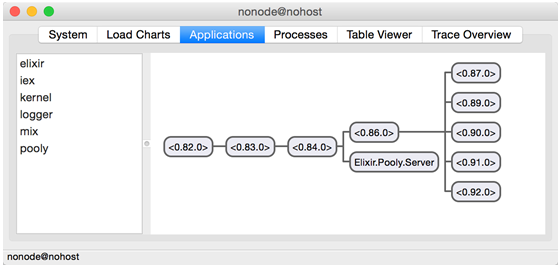
\includegraphics[width=0.8\linewidth]{6_4a.png}
    \caption{从 Observer 看到的 Pooly 的版本 1}
    \label{fig:6_4a}
\end{figure}


让我们开始杀死一个
worker。(我希望你没有大声朗读这本书)。你可以通过右键点击一个 worker
进程并选择 \emph{Kill process} 来做到这一点:

\begin{figure}[!ht]
    \centering
    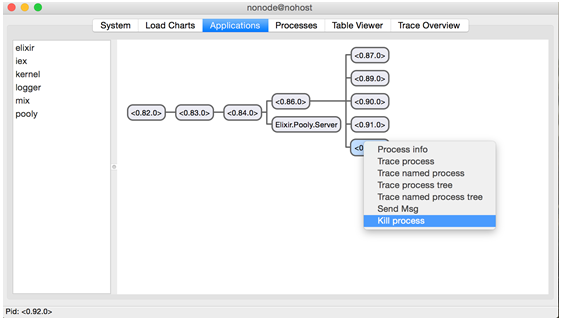
\includegraphics[width=0.8\linewidth]{6_5.png}
    \caption{从 Observer 杀死 worker}
    \label{fig:6_5}
\end{figure}

你会发现,监督器在被杀死的进程的位置生成了一个新的 worker。

更重要的是,单个 worker
的崩溃/退出并没有影响到监督树的其余部分。换句话说,那个单独的 worker
的崩溃只影响到\emph{那个} worker,而没有影响到其他任何东西。

\begin{figure}[!ht]
    \centering
    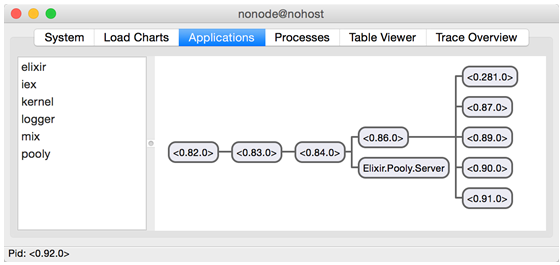
\includegraphics[width=0.8\linewidth]{6_6.png}
    \caption{监督器用新生成的 worker 替换了被杀死的 worker}
    \label{fig:6_6}
\end{figure}

现在,如果我们杀死 \texttt{Pooly.Server}
会发生什么呢?再次,右键点击 \texttt{Pooly.Server}
并选择 \emph{Kill process},就像这样:

\begin{figure}[!ht]
    \centering
    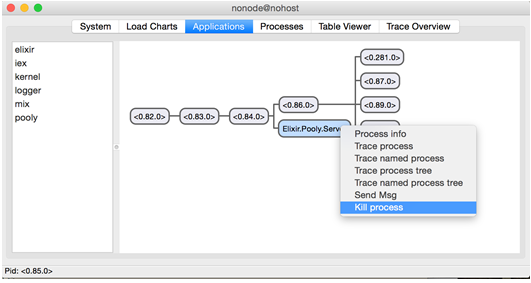
\includegraphics[width=0.8\linewidth]{6_7.png}
    \caption{从 Observer 杀死 Server 进程}
    \label{fig:6_7}
\end{figure}


这次,\emph{所有}的进程都被杀死,顶级监督器重新启动了\emph{所有}的子进程:

\begin{figure}[!ht]
    \centering
    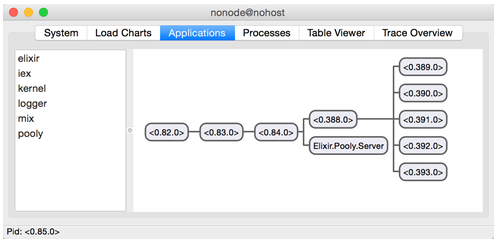
\includegraphics[width=0.8\linewidth]{6_8.png}
    \caption{杀死 Server 重新启动了顶级监督器下的所有进程}
    \label{fig:6_8}
\end{figure}


刚刚发生了什么?为什么杀死 \texttt{Pooly.Server}
会导致顶级监督器下的所有东西都死掉?仅仅是效果的描述就应该已经给出了一个重要的线索。顶级监督器的重启策略是什么?

让我们稍微回忆一下:

\begin{code}{}
\begin{minted}[linenos]{elixir}
defmodule Pooly.Supervisor do
  def init(pool_config) do
    # …
    opts = [strategy: :one_for_all]

    supervise(children, opts)
  end
end
\end{minted}
% \label{lst:id}
\end{code}

\texttt{:one\_for\_all} 重启策略完全解释了为什么杀死
\texttt{Pooly.Server}
会导致(并重新启动)其余的所有子进程。

 \section{练习}

\begin{enumerate}
\def\labelenumi{\arabic{enumi}.}
\item
  当你在 Observer 中杀死 \texttt{WorkerSupervisor}
  进程时会发生什么?你能解释发生了什么吗?
\item
  关闭和重启值。尝试使用各种关闭和重启值。例如,在
  \texttt{Pooly.WorkerSupervisor} 中,尝试将
  \texttt{opts} 从
\end{enumerate}

\begin{code}{}
\begin{minted}[linenos]{elixir}
opts = [strategy: :simple_one_for_one, max_restarts: 5, max_seconds: 5]
\end{minted}
% \label{lst:id}
\end{code}

改为类似于

\begin{code}{}
\begin{minted}[linenos]{elixir}
opts = [strategy: :simple_one_for_one, max_restarts: 0, max_seconds: 5]
\end{minted}
% \label{lst:id}
\end{code}

接下来,尝试将 \texttt{worker\_opts} 从

\begin{code}{}
\begin{minted}[linenos]{elixir}
worker_opts = [restart:  :permanent, function: f]
\end{minted}
% \label{lst:id}
\end{code}

改为

\begin{code}{}
\begin{minted}[linenos]{elixir}
worker_opts = [restart:  :temporary, function: f]
\end{minted}
% \label{lst:id}
\end{code}

记住要将 \texttt{opts} 设置回原始值。

 \section{总结}

在本章中,我们学习了:

\begin{itemize}

\item
  OTP Supervisor 行为
\item
  不同的监督器重启策略
\item
  使用 ETS 存储状态
\item
  如何构建监督器层次结构,包括静态和动态
\item
  各种监督器和子进程规范选项
\item
  实现一个非常基础的 worker 池应用程序
\end{itemize}

我们已经看到,通过使用不同的重启策略,监督器可以决定其子进程如何重启。更重要的是,再次依赖于重启策略,监督器能够将崩溃隔离到仅受影响的进程。

尽管 Pooly
的第一个版本很简单,但它让我们有机会尝试构建静态和动态的监督器层次结构。在前一种情况中,我们在
\texttt{Pooly.Supervisor} 的监督规范中声明
\texttt{Pooly.Server}
应该被监督。在后一种情况中,只有当
\texttt{Pooly.Server}
初始化时,\texttt{Pooly.WorkerSupervisor}
才会被添加到监督树中。

在接下来的章节中,我们将继续发展 Pooly
的设计,同时为其添加更多功能。同时,我们将探索 Supervisor 的更高级用法。

\protect\hyperlink{u7YNvHigi67GoJPRzPXBQf4}{****{[}1{]}****} 这是以 Mr.T的口气写的。
\protect\hyperlink{unZsK4dstzhrpK6CA9DbDs8}{****{[}2{]}****} 
\protect\hyperlink{u5UHZe9erUMjrZtCEGXEoxG}{****{[}3{]}****}
这在软件行业是很少见的。

/printnotes
\chapter{完成工作池应用程序}\label{chapt:worker-pool}

本章内容包括:

\begin{enumerate}
	\item 实现完整的工作池应用程序
  \item 构建多个监督层级
  \item 动态创建监督者和工作者
\end{enumerate}

在本章中,我们将继续发展在第 6 章开始的 \texttt{Pooly}的设计。
到本章结束时,我们将拥有一个完整且功能齐全的工作池应用程序。
我们将更深入地探索Supervisor API,并探讨更高级(也就是更有趣!)的监督者主题。

在第\ref{chapt:fault-tolerent}章中,我们停留在一个非常基础的工作池应用程序阶段,如果可以这样说的话。
在接下来的部分中,我们将为\texttt{Pooly}添加一些智能。
例如,目前还没有办法优雅地处理崩溃和重启。\texttt{Pooly}的当前版本只能处理单个池和固定数量的工作者。
第 3 版本的\texttt{Pooly}将实现对多个池的支持,以及对可变数量的工作进程的支持。

有时池需要处理意外负载。当请求太多时会发生什么?当所有工作者都忙时会发生什么?
在第4 版中,我们使池具有可变大小,允许工作者的\emph{溢出}。
我们还实现了在所有工作者都忙时对消费者进程的排队。

\section{版本3:错误处理、多个池和工作者}

我们如何知道一个进程崩溃了?我们可以监视或链接它。这引出了下一个问题,我们应该选择哪一个?为了回答这个问题,我们必须思考当进程崩溃时应该发生什么。有两种情况需要考虑。崩溃可能发生在:

· 服务器进程和消费者进程之间

· 服务器进程和工作者进程之间


\subsection{情况1:服务器和工作者之间的崩溃}

服务器进程的崩溃不应该影响消费者进程。事实上,反之亦然!当消费者进程崩溃时,它不应该使服务器进程崩溃。因此,\emph{监视器}
是正确的选择。

每次工作者检出时,我们已经在监视消费者进程。剩下的就是处理消费者进程的\texttt{:DOWN} 消息:

\begin{code}{lib/pooly/server.ex – 处理消费者进程的 :DOWN 消息}

\begin{minted}[linenos]{elixir}
defmodule Pooly.Server do
  #############
  # Callbacks #
  #############

  def handle_info({:DOWN, ref, _, _, _}, state = %{monitors: monitors, workers: workers}) do
    case :ets.match(monitors, {:"$1", ref}) do
      [[pid]] ->
        true = :ets.delete(monitors, pid)
        # 1
        new_state = %{state | workers: [pid | workers]}
        {:no_reply, new_state}

      [[]] ->
        {:no_reply, state}
    end
  end
end

# 1 将工作者返回到池中
\end{minted}
\label{lst:worker-pool-handle-info}
\end{code}

当消费者进程崩溃时,我们在 \texttt{monitors} ETS表中匹配引用,删除监视器,并将工作者添加回状态中。


\subsection{情况2:服务器和工作者之间的崩溃}

如果服务器崩溃,它应该带下工作者进程吗?应该,因为否则,服务器的状态将与池的实际状态不一致。
另一方面,当工作者进程崩溃时,它应该使服务器进程崩溃吗?当然不是!这对我们意味着什么?
嗯,由于双向依赖,我们应该使用\emph{链接}。然而,由于服务器在工作者进

程崩溃时 \emph{不应} 崩溃,服务器进程应该捕获退出:

\begin{code}{}
\begin{minted}[linenos]{elixir}
defmodule Pooly.Server do
  #############
  # Callbacks #
  #############
  def init([sup, pool_config]) when is_pid(sup) do
    # 1
    Process.flag(:trap_exit, true)
    monitors = :ets.new(:monitors, [:private])
    init(pool_config, %State{sup: sup, monitors: monitors})
  end
end

# 1 设置服务器进程以捕获退出。
\end{minted}
% \label{lst:id}
\end{code}

现在服务器进程已经开始捕获退出,我们应该处理来自工作者的
\texttt{:EXIT} 消息:

\begin{code}{}
\begin{minted}[linenos]{elixir}
defmodule Pooly.Server do
  #############
  # Callbacks #
  #############

  def handle_info(
        {:EXIT, pid, _reason},
        state = %{monitors: monitors, workers: workers, worker_sup: worker_sup}
      ) do
    case :ets.lookup(monitors, pid) do
      [{pid, ref}] ->
        true = Process.demonitor(ref)
        true = :ets.delete(monitors, pid)
        new_state = %{state | workers: [new_worker(worker_sup) | workers]}
        {:noreply, new_state}

      [[]] ->
        {:noreply, state}
    end
  end
end
\end{minted}
% \label{lst:id}
\end{code}

当工作者进程意外退出时,在 \texttt{monitors} ETS
表中查找其条目。如果条目不存在,则无需执行任何操作。否则,不再监视消费者进程,并从
\texttt{monitors}
表中删除其条目。最后,创建一个新的工作者并将其添加回服务器状态的工作者字段中。

 \subsection{ 处理多个池}

在第 2
版之后,我们有了一个非常基本的工作池。然而,任何自尊的工作池应用程序都应该能够处理多个池。在我们开始编码之前,让我们先考虑一些可能的设计。最直接的方法是这样设计监督树:

\begin{figure}[!ht]
    \centering
    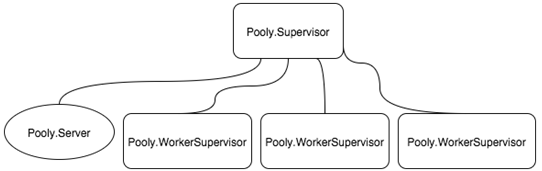
\includegraphics[width=0.8\linewidth]{7_1.png}
    \caption{处理多个池的可能设计}
    \label{fig:7_1}
\end{figure}


你看到问题了吗?我们实际上是在
\texttt{Pooly.Supervisor} 中添加更多的
\texttt{WorkerSupervisor}。这是一个糟糕的设计。问题在于
\emph{错误核心},或者说缺乏错误核心。

请允许我详细说明。任何 \texttt{WorkerSupervisor}
的问题都不应该影响
\texttt{Pooly.Server}。思考当一个进程崩溃时会发生什么,以及谁会受到影响是值得的。一个潜在的修复方法可能是添加另一个监督者来处理所有工作者监督者,比如
\texttt{Pooly.WorkersSupervisor}(\emph{只是}
另一个间接层!)。现在它可能是这样的:

\begin{figure}[!ht]
    \centering
    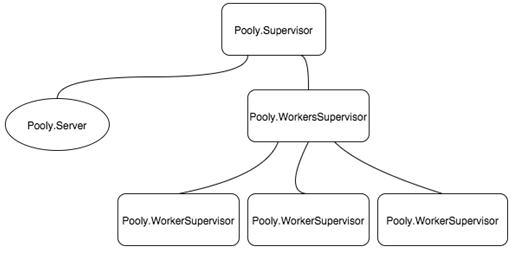
\includegraphics[width=0.8\linewidth]{7_2.png}
    \caption{另一种可能的设计。你能识别出瓶颈吗?}
    \label{fig:7_2}
\end{figure}


你注意到另一个问题了吗?可怜的 \texttt{Pooly.Server}
必须处理 \emph{每个}
池的所有请求。这意味着如果消息快速而猛烈地发送到服务器进程,可能会导致服务器进程成为瓶颈,并可能淹没其邮箱。\texttt{Pooly.Server}
也是单点故障,因为它包含每个池的状态。服务器进程的死亡意味着 \emph{所有}
工作者监督者都必须被关闭。那么考虑一下这个设计:

\begin{figure}[!ht]
    \centering
    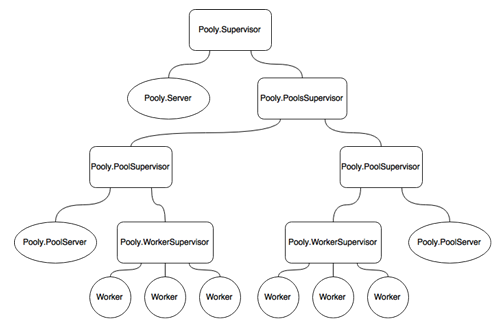
\includegraphics[width=0.8\linewidth]{7_3.png}
    \caption{Pooly 的最终设计}
    \label{fig:7_3}
\end{figure}



\subsubsection{顶层监督器}

\texttt{Pooly.Supervisor} 作为顶层监督器,管理一个
\texttt{Pooly.Server} 和一个
\texttt{PoolsSupervisor}。\texttt{PoolsSupervisor}
又管理多个 \texttt{PoolSupervisor}。每个
\texttt{PoolSupervisor} 管理自己的
\texttt{PoolServer} 和
\texttt{WorkerSupervisor}。

如你所猜测的,Pooly将进行设计大修。为了便于跟踪,我们将从上到下实施更改。


\subsection{添加应用行为到 Pooly}

首先要更改的地方是
\texttt{lib/pooly.ex},Pooly的主入口。由于我们现在支持多个池(pool),我们希望通过其名称引用每个池。这意味着各种函数也将接受
\texttt{pool\_name} 作为参数:


\subparagraph{代码 7.4 lib/pooly.ex -
添加对多个池的支持}

\begin{code}{}
\begin{minted}[linenos]{elixir}
defmodule Pooly do
  use Application

  def start(_type, _args) do
    # 2
    # 1
    pools_config =
      [
        # 1
        [
          name: "Pool1",
          # 1
          mfa: {SampleWorker, :start_link, []},
          size: 2
        ],
        # 1
        [
          name: "Pool2",
          # 1
          mfa: {SampleWorker, :start_link, []},
          size: 3
        ],
        # 1
        [
          name: "Pool3",
          # 1
          mfa: {SampleWorker, :start_link, []},
          size: 4
        ]
      ]

    # 1

    # 2
    start_pools(pools_config)
  end

  # 2
  def start_pools(pools_config) do
    # 2
    Pooly.Supervisor.start_link(pools_config)
  end

  # 3
  def checkout(pool_name) do
    # 3
    Pooly.Server.checkout(pool_name)
  end

  # 3
  def checkin(pool_name, worker_pid) do
    # 3
    Pooly.Server.checkin(pool_name, worker_pid)
  end

  # 3
  def status(pool_name) do
    # 3
    Pooly.Server.status(pool_name)
  end
end

# 1 池配置现在接受多个池的配置。池也有名称。
# 2 从 pool\_config 到 pools\_config 的复数变化。
# 3 其余的 API 接受 pool\_name 作为参数。
\end{minted}
% \label{lst:id}
\end{code}




\subsection{添加顶层监督器}

我们的下一站是顶层监督器,\texttt{lib/pooly/supervisor.ex}。顶层监督器负责启动
\texttt{Pooly.Server} 和
\texttt{Pooly.PoolsSupervisor}。当
\texttt{Pooly.PoolsSupervisor} 启动时,它启动各自的
\texttt{Pooly.PoolSupervisor},而这些又启动它们自己的
\texttt{Pooly.Server} 和
\texttt{Pooly.WorkerSupervisor}。


\begin{figure}[!ht]
    \centering
    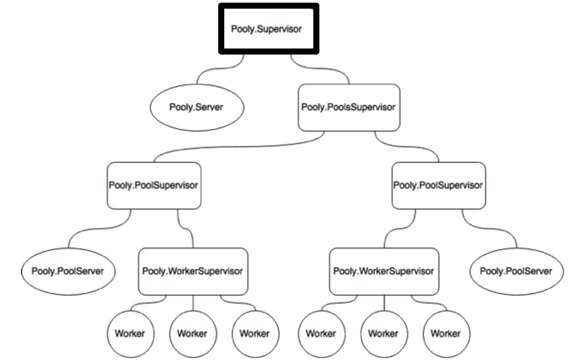
\includegraphics[width=0.8\linewidth]{7_4.png}
    \caption{从顶层监督器开始}
    \label{fig:7_4}
\end{figure}


看图,\texttt{Pooly.Supervisor}
监督两个进程:\texttt{Pooly.PoolsSupervisor}(尚未实现)和
\texttt{Pooly.Server}。因此,我们需要将这两个进程添加到
\texttt{Pooly.Supervisor}
的子进程列表中。我们就这样做:


\subparagraph{代码 7.5 lib/pooly/supervisor.ex --
顶层监督器监督顶层池服务器和池监督器}

\begin{code}{}
\begin{minted}[linenos]{elixir}
defmodule Pooly.Supervisor do
  use Supervisor

  def start_link(pools_config) do                       #1
    Supervisor.start_link(__MODULE__, pools_config,
                          name: __MODULE__)             #2
  end

  def init(pools_config) do                             #1
    children = [
      supervisor(Pooly.PoolsSupervisor, []),            #3
      worker(Pooly.Server, [pools_config])              #3
    ]

    opts = [strategy: :one_for_all]

    supervise(children

, opts)
  end
end

#1 从 pool\_config 到 pools\_config 的复数变化。
#2 Pooly.Supervisor 现在是一个命名进程。
#3 Pooly.Supervisor 现在监督两个子进程。注意 Pooly.Server 不再需要Pooly.Supervisor 的 pid,因为我们可以通过名称引用它。
\end{minted}
% \label{lst:id}
\end{code}

\texttt{Pooly.Supervisor} 的主要变化是添加
\texttt{Pooly.PoolsSupervisor} 作为子进程,并给
\texttt{Pooly.Supervisor} 命名。回想一下,我们在 \#1
中将 \texttt{Pooly.Supervisor} 的名称设置为
\texttt{\_\_MODULE\_\_},这意味着我们可以将进程引用为
\texttt{Pooly.Supervisor} 而不是
pid。因此,我们不需要将 \texttt{self}(参见
\texttt{Pooly.Supervisor} 的第二版)传递给
\texttt{Pooly.Server}。


\subsection{添加池的监督器}

在 \texttt{lib/pooly/} 下创建
\texttt{pools\_supervisor.ex}。以下是实现:


\subparagraph{代码 7.6 lib/pooly/pools\_supervisor.ex --
池监督器的完整实现}

\begin{code}{}
\begin{minted}[linenos]{elixir}
defmodule Pooly.PoolsSupervisor do
  use Supervisor

  def start_link do
    # 1
    Supervisor.start_link(__MODULE__, [], name: __MODULE__)
  end

  def init(_) do
    opts = [
      # 2
      strategy: :one_for_one
    ]

    supervise([], opts)
  end
end
\end{minted}
% \label{lst:id}
\end{code}

就像 \texttt{Pooly.Supervisor},我们给
\texttt{Pooly.PoolsSupervisor}
命名。注意这个监督器没有子规格。事实上,当它启动时,没有任何池附加到它。这是因为,就像版本
2
一样,我们想在创建任何池之前验证池配置。因此,我们提供的唯一信息是重启策略,如
\#2 所示。为什么是
\texttt{:one\_for\_one}?任何池的崩溃都不应该影响其他池。

\subsection{使 Pooly.Server 更简单}

在第一版和第二版中,我们说 \texttt{Pooly.Server}
是整个操作的大脑。但现在不再是这样了。\texttt{Pooly.Server}
的一些工作将由专门的 \texttt{Pooly.PoolServer} 接管。

\begin{figure}[!ht]
\centering
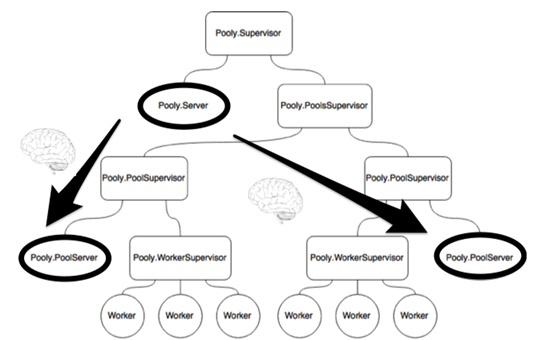
\includegraphics[width=0.8\linewidth]{7_6.png}
\caption{从之前版本的顶级池服务器中移动的逻辑将被移至各个池服务器}
\end{figure}

图 7.6 从之前版本的顶级池服务器中移动的逻辑将被移至各个池服务器

大多数 API 与之前版本相同,增加了
\texttt{pool\_name}。打开
\texttt{lib/pooly/server.ex}
并\emph{替换}之前的实现为以下内容:

\begin{code}{lib/pooly/server.ex - 顶级池服务器的完整实现}

\begin{minted}[linenos]{elixir}
defmodule Pooly.Server do
  use GenServer
  import Supervisor.Spec

  ####### 
  # API #
  #######

  def start_link(pools_config) do
    GenServer.start_link(__MODULE__, pools_config, name: __MODULE__)
  end

  def checkout(pool_name) do
    # 2
    GenServer.call(:"#{pool_name}Server", :checkout)
  end

  def checkin(pool_name, worker_pid) do
    # 2
    GenServer.cast(:"#{pool_name}Server", {:checkin, worker_pid})
  end

  def status(pool_name) do
    # 2
    GenServer.call(:"#{pool_name}Server", :status)
  end

  #############
  # Callbacks #
  #############

  # 3
  def init(pools_config) do
    # 3
    pools_config
    |> Enum.each(fn pool_config ->
      # 3
      send(self, {:start_pool, pool_config})
    end)

    # 3

    {:ok, pools_config}
  end

  # 4
  def handle_info({:start_pool, pool_config}, state) do
    # 4
    {:ok, _pool_sup} = Supervisor.start_child(Pooly.PoolsSupervisor, supervisor_spec(pool_config))
    {:no_reply, state}
  end

  #####################
  # Private Functions #
  #####################

  defp supervisor_spec(pool_config) do
    # 5
    opts = [id: :"#{pool_config[:name]}Supervisor"]
    supervisor(Pooly.PoolSupervisor, [pool_config], opts)
  end
end
\end{minted}
% \label{lst:id}
\end{code}

在这个版本中,\texttt{Pooly.Server}
的工作是\emph{委托}所有请求给相应的池,并启动池并将池附加到
\texttt{Pooly.PoolsSupervisor}。

在 \#2 中,我们假设每个单独的池服务器被命名为
\texttt{:"\#\{pool\_name\}Server"}。注意名字是\emph{原子}!遗憾的是,因为我未能正确阅读文档,我在这上面浪费了几个小时(和头发)。

在 \#3 中,\texttt{pools\_config} 被迭代,发送
\mintinline{elixir}|{:start_pool, pool\_config}| 消息给自己。在
\#4 中处理消息,告诉 \texttt{Pooly.PoolsSupervisor}
根据给定的 \texttt{pool\_config} 启动一个子进程。

这里有一个\emph{微小}的注意点。注意在 \#5 中我们确保每个
\texttt{Pooly.PoolSupervisor} 以\emph{独特}的监督器规范
id 启动。如果忘记这样做,你会得到一个如下的神秘错误信息:

\begin{code}{}
\begin{minted}[linenos]{elixir}
12:08:16.336 [error] GenServer Pooly.Server terminating
Last message: {:start_pool, [name: "Pool2", mfa: {SampleWorker, :start_link, []}, size: 2]}
State: [[name: "Pool1", mfa: {SampleWorker, :start_link, []}, size: 2], [name: "Pool2", mfa: {SampleWorker, :start_link, []}, size: 2]]
** (exit) an exception was raised:
** (MatchError) no match of right hand side value: {:error, {:already_started, #PID<0.142.0>}}
(pooly) lib/pooly/server.ex:38: Pooly.Server.handle_info/2
(stdlib) gen_server.erl:593: :gen_server.try_dispatch/4
(stdlib) gen_server.erl:659: :gen_server.handle_msg/5
(stdlib

) proc_lib.erl:237: :proc_lib.init_p_do_apply/3
\end{minted}
% \label{lst:id}
\end{code}

这里的线索是
\mintinline{elixir}|{:error, \{:already_started, \#PID<0.142.0>\}}|。我花了几个小时试图解决这个问题,直到偶然发现这个解决方案。当一个
\texttt{Pooly.PoolSupervisor} 以给定的
\texttt{pool\_config} 启动时会发生什么?

\subsection{添加池监督器}

\begin{figure}[!ht]
    \centering
    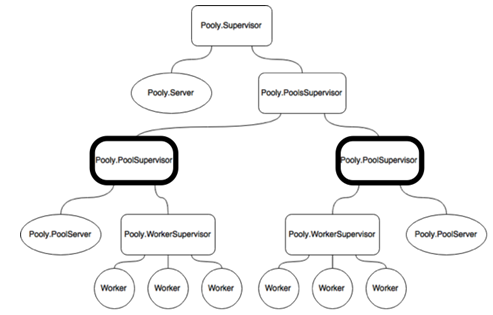
\includegraphics[width=0.8\linewidth]{7_7.png}
    \caption{实现各个池监督器}
    \label{fig:7_7}
\end{figure}

\texttt{Pooly.PoolSupervisor} 取代了之前版本的
\texttt{Pooly.Supervisor}。因此,只有一些小的更改。首先,每个
\texttt{Pooly.PoolSupervisor}
现在都初始化了一个名字。其次,我们需要告诉
\texttt{Pooly.PoolSupervisor} 使用
\texttt{Pooly.PoolServer}。以下是更改内容:

\begin{code}{lib/pooly/pool\_supervisor.ex - 单个池监督器的完整实现}

\begin{minted}[linenos]{elixir}
defmodule Pooly.PoolSupervisor do
  use Supervisor

  def start_link(pool_config) do
    # 1
    Supervisor.start_link(__MODULE__, pool_config, name: :"#{pool_config[:name]}Supervisor")
  end

  def init(pool_config) do
    opts = [
      strategy: :one_for_all
    ]

    children = [
      # 2
      worker(Pooly.PoolServer, [self, pool_config])
    ]

    supervise(children, opts)
  end
end
\end{minted}
% \label{lst:id}
\end{code}

我们在 \#1
中给单个池监督器命名,尽管这并非严格必要。这有助于我们在观察器中轻松找到池监督器。

其次,\#2 中的子进程规范从 \texttt{Pooly.Server} 更改为
\texttt{Pooly.PoolServer}。我们传递相同的参数。尽管我们正在命名
\texttt{Pooly.PoolSupervisor},我们将\emph{不会}在
\texttt{Pooly.PoolServer}
中使用该名称,这样我们可以重用来自版本2的
\texttt{Pooly.Server} 的大部分实现。


\subsection{添加池(Pool)的核心逻辑}

如上一节所述,大部分逻辑保持不变,只是在一些地方进行了修改以支持多个池。为了节约纸张和屏幕空间,与\texttt{Pooly.Server}版本2完全相同的函数被用``\texttt{\# …}''标记了出来。换句话说,如果你在跟随学习,可以将\texttt{Pooly.Server}版本2的实现复制粘贴到\texttt{Pooly.PoolyServer}。

以下是\texttt{Pooly.PoolServer}的实现:



\begin{code}{代码 7.9 lib/pooly/pool\_server.ex -单个池服务器的完整实现}

\begin{minted}[linenos]{elixir}
defmodule Pooly.PoolServer do
  use GenServer
  import Supervisor.Spec

  defmodule State do
    defstruct pool_sup: nil,
              worker_sup: nil,
              monitors: nil,
              size: nil,
              workers: nil,
              name: nil,
              mfa: nil
  end

  def start_link(pool_sup, pool_config) do
    GenServer.start_link(__MODULE__, [pool_sup, pool_config], name: name(pool_config[:name]))
  end

  def checkout(pool_name) do
    GenServer.call(name(pool_name), :checkout)
  end

  def checkin(pool_name, worker_pid) do
    GenServer.cast(name(pool_name), {:checkin, worker_pid})
  end

  def status(pool_name) do
    GenServer.call(name(pool_name), :status)
  end

  # 回调函数
  # ...

  def init([pool_sup, pool_config]) when is_pid(pool_sup) do
    Process.flag(:trap_exit, true)
    monitors = :ets.new(:monitors, [:private])
    init(pool_config, %State{pool_sup: pool_sup, monitors: monitors})
  end

  def init([{:name, name} | rest], state) do
    # …
  end

  # 其他初始化函数
  # ...

  def handle_call(:checkout, {from_pid, _ref}, %{workers: workers, monitors: monitors} = state) do
    # …
  end

  def handle_call(:status, _from, %{workers: workers, monitors: monitors} = state) do
    # …
  end

  def handle_cast({:checkin, worker}, %{workers: workers, monitors: monitors} = state) do
    # …
  end

  def handle_info(
        :start_worker_supervisor,
        state = %{pool_sup: pool_sup, name: name, mfa: mfa, size: size}
      ) do
    {:ok, worker_sup} = Supervisor.start_child(pool_sup, supervisor_spec(name, mfa))
    workers = prepopulate(size, worker_sup)
    {:no_reply, %{state | worker_sup: worker_sup, workers: workers}}
  end

  def handle_info({:DOWN, ref, _, _, _}, state = %{monitors: monitors, workers: workers}) do
    # …
  end

  # 其他处理函数
  # ...

  def terminate(_reason, _state) do
    :ok
  end

  # 私有函数
  # ...

  defp name(pool_name) do
    :"#{pool_name}Server"
  end

  defp prepopulate(size, sup) do
    # …
  end

  # 其他预填充函数
  # ...

  defp supervisor_spec(name, mfa) do
    opts = [id: name <> "WorkerSupervisor", restart: :temporary]
    supervisor(Pooly.WorkerSupervisor, [self, mfa], opts)
  end
end
\end{minted}
% \label{lst:id}
\end{code}

这里有几个显著的变化。服务器的\texttt{start\_link/2}函数将\emph{池监督器}作为第一个参数。在\#3中,池监督器的pid被保存在服务器进程的状态中。此外,注意服务器的状态已扩展以存储池监督器和工作监督器的pid:

\begin{code}{}
\begin{minted}[linenos]{elixir}
defmodule State do
  defstruct pool_sup: nil,
            worker_sup: nil,
            monitors: nil,
            size: nil,
            workers: nil,
            name: nil,
            mfa: nil
end
\end{minted}
% \label{lst:id}
\end{code}

一旦服务器处理完池配置,它将最终向自己发送\texttt{:start\_worker\_supervisor}消息,如\#4所示。这条消息由\texttt{handle\_info/2}回调处理。在

\#5中,池监督器被告知作为子项启动工作监督器,使用\#8中定义的子进程规范。除了\texttt{mfa},我们还传递了服务器进程的pid。一旦返回工作监督器的pid,它就会在\#6中被用来预填充\texttt{Worker}。\#2利用\texttt{name/1}来引用适当的池服务器以调用相应的函数。

\subsection{为池添加工作监管器}

最后一部分是工作监管器。它负责管理单个工作程序。它管理任何崩溃的工作程序。有一个微妙的细节。在初始化期间,工作监管器创建了与其对应池服务器的\emph{链接}。为什么要这样做?如果池服务器或工作监管器中的任何一个停止工作,另一个继续存在就没有意义了。

\begin{figure}[!ht]
    \centering
    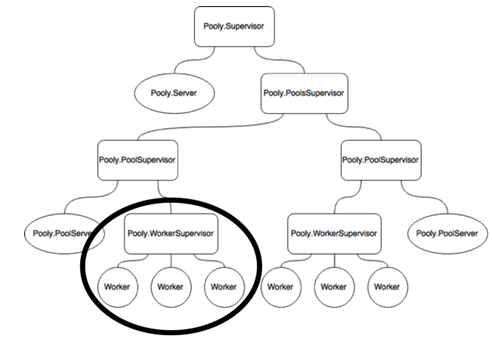
\includegraphics[width=0.8\linewidth]{7_8.png}
    \caption{实现单个池的工作监管器}
    \label{fig:7_8}
\end{figure}


让我们看看完整实现的更多细节:

代码代码 7.10 lib/pooly/worker\_supervisor.ex --
池的工作监管器的完整实现

\begin{code}{}
\begin{minted}[linenos]{elixir}
defmodule Pooly.WorkerSupervisor do
  use Supervisor

  # 1
  def start_link(pool_server, {_, _, _} = mfa) do
    # 1
    Supervisor.start_link(__MODULE__, [pool_server, mfa])
  end

  def init([pool_server, {m, f, a}]) do
    # 2
    Process.link(pool_server)
    worker_opts = [restart: :temporary, shutdown: 5000, function: f]

    children = [worker(m, a, worker_opts)]
    opts = [strategy: :simple_one_for_one, max_restarts: 5, max_seconds: 5]

    supervise(children, opts)
  end
end
\end{minted}
% \label{lst:id}
\end{code}

唯一的变化是增加了额外的\texttt{pool\_server}参数,并将\texttt{pool\_server}与工作监管器进程链接。为什么?如前所述,这两个进程之间存在依赖关系,当工作监管器停止工作时,需要通知池服务器。同样,如果工作监管器崩溃,它也应该同时带下池服务器。

为了让池服务器处理这个消息,你需要在\texttt{lib/pooly/pool\_server.ex}中添加另一个\texttt{handle\_info/2}回调:

代码代码 7.11 lib/pooly/pool\_server.ex --
让池服务器检测到工作监管器停止工作

\begin{code}{}
\begin{minted}[linenos]{elixir}
defmodule Pooly.PoolServer do
  #############
  # Callbacks #
  #############

  def handle_info({:EXIT, worker_sup, reason}, state = %{worker_sup: worker_sup}) do
    {:stop, reason, state}
  end
end
\end{minted}
% \label{lst:id}
\end{code}

在这里,每当工作监管器退出时,它也会终止池服务器,并且原因是与终止工作监管器的原因相同。

\subsection{将其实际运行}

让我们确保我们正确地连接了一切。首先,打开\texttt{lib/pooly.ex}来配置池。确保\texttt{start/2}函数看起来像这样:

代码\begin{code}{lib/pooly.ex -- 配置 Pooly 启动三个不同大小的池}

\begin{minted}[linenos]{elixir}
defmodule Pooly do
use Application

def start(_type, _args) do
pools_config =
[
[name: "Pool1", mfa: {SampleWorker, :start_link, []}, size: 2],
[name: "Pool2", mfa: {SampleWorker, :start_link, []}, size: 3],
[name: "Pool3", mfa: {SampleWorker, :start_link, []}, size: 4]
]

start_pools(pools_config)
end

# …end
\end{minted}
% \label{lst:id}
\end{code}

在这里,我们告诉 Pooly
创建三个池,每个池具有给定的大小和工作类型。为了简单(实际上是懒惰),我们在所有三个池中都使用了\texttt{SampleWorker}。在一个新的终端会话中,启动\texttt{iex}并启动
Observer:

\begin{code}{}
\begin{minted}[linenos]{elixir}
% iex -S mix
iex> :observer.start
\end{minted}
% \label{lst:id}
\end{code}

见证你所创建的壮丽监管树:

\begin{figure}[!ht]
    \centering
    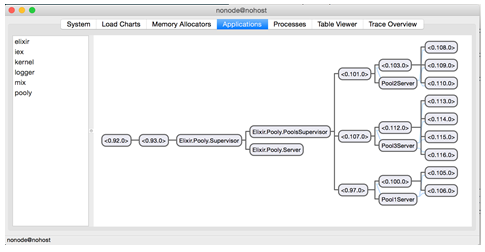
\includegraphics[width=0.8\linewidth]{7_9.png}
    \caption{从 Observer 看到的 Pooly 监管树}
    \label{fig:7_9}
\end{figure}


现在,从监管树的叶子(最低/最右边)开始,

尝试右击进程并杀死它。你会再次注意到一个新进程会接管。

接下来,往上走。比如,当杀死\texttt{Pool3Server}时会发生什么?你会注意到对应的\texttt{WorkerSupervisor}和它下面的工作程序都会被杀死并重新生成。重要的是要注意,\texttt{Pool3Server}是一个全新的进程。

现在再往上走。当你杀死一个\texttt{PoolSupervisor}时会发生什么?正如预期的那样,它下面的所有东西都会被杀死,另一个\texttt{PoolSupervisor}会重新生成,它下面的所有东西也会重新生成。注意不会发生的事情。应用程序的其余部分不会受到影响。这不是很棒吗?当崩溃发生时,正如它们不可避免地会发生的那样,拥有一个精心层次化的监管层次结构可以让错误以非常孤立的方式处理,从而不影响应用程序的其余部分。

\section{版本 4:实现溢出和排队功能}

在 Pooly
的最终版本中,我们将扩展它以支持可变数量的工作进程,方法是指定一个\emph{最大溢出量}。

我们还希望引入\emph{排队}工作进程的概念。也就是说,当达到最大溢出限制时,Pooly
能够为愿意\emph{阻塞并等待}下一个可用工作进程的消费者排队工作进程。

\subsection{实现最大溢出}

像往常一样,为了指定最大溢出,我们在池配置中添加了一个新字段。在
\texttt{lib/pooly.ex} 中,修改
\texttt{start/2} 中的
\texttt{pools\_config},使其看起来如下:

\begin{code}{lib/pooly.ex - 实现最大溢出}

\begin{minted}[linenos]{elixir}
defmodule Pooly do

def start(_type, _args) do
pools_config =
[
[name: "Pool1",
mfa: {SampleWorker, :start_link, []},
size: 2,
max_overflow: 3                       #1
],
[name: "Pool2",
mfa: {SampleWorker, :start_link, []},
size: 3,
max_overflow: 0                       #1
],
[name: "Pool3",
mfa: {SampleWorker, :start_link, []},
size: 4,
max_overflow: 0                       #1
]
]

start_pools(pools_config)
end
end
#1 在池配置中指定最大溢出。
\end{minted}
% \label{lst:id}
\end{code}


现在我们有了池配置的新选项,我们必须前往
\texttt{lib/pooly/pool\_server.ex} 以支持
\texttt{max\_overflow}。这包括:

· 在 \texttt{State} 中添加一个名为
\texttt{max\_overflow} 的条目

· 在 \texttt{State} 中添加一个名为
\texttt{overflow} 的条目,用于跟踪当前溢出计数

· 在 \texttt{init/2} 中添加一个函数子句来处理
\texttt{max\_overflow}

以下是添加内容:

\begin{code}{lib/pooly/pool\_server.ex - 在池服务器中添加最大溢出选项}

\begin{minted}[linenos]{elixir}
defmodule Pooly.PoolServer do
  defmodule State do
    defstruct pool_sup: nil,
              worker_sup: nil,
              monitors: nil,
              size: nil,
              workers: nil,
              name: nil,
              mfa: nil,
              overflow: nil,
              max_overflow: nil
  end

  #############
  # Callbacks #
  #############

  def init([{:name, name} | rest], state) do
    # …
  end

  # … more init/1 definitions

  def init([{:max_overflow, max_overflow} | rest], state) do
    init(rest, %{state | max_overflow: max_overflow})
  end

  def init([], state) do
    # …
  end

  def init([_ | rest], state) do
    # …
  end
end
\end{minted}
% \label{lst:id}
\end{code}

接下来,我们必须考虑实际溢出的情况。当忙碌工作进程的总数超过
\texttt{size} \emph{并且} 在
\texttt{max\_overflow}
限制内时,就会发生溢出。何时会发生溢出?当工作进程被\emph{取出}时。因此,唯一需要查看的地方是
\texttt{handle\_call(\{:checkout, block\}, from, state)}。

处理这种情况相当简单。\#1
检查我们是否在溢出限制内。如果是,将创建一个新的工作进程,并将必要的簿记信息添加到
\texttt{monitors} ETS 表中。然后将工作进程 pid
作为回复发送给消费者进程,并增加 \texttt{overflow}
计数:

\begin{code}{lib/pooly/pool\_server.ex - 在池服务器中处理取出时的溢出}

\begin{minted}[linenos]{elixir}
defmodule Pooly.PoolServer do
  #############
  # Callbacks #
  #############

  def handle_call({:checkout, block}, {from_pid, _ref} = from, state) do
    %{
      worker_sup: worker_sup,
      workers: workers,
      monitors: monitors,
      overflow: overflow,
      max_overflow: max_overflow
    } = state

    case workers do
      [worker | rest] ->
        # …
        {:reply, worker, %{state | workers: rest}}

      # 1
      [] when max_overflow > 0 and overflow < max_overflow ->
        {worker, ref} = new_worker(worker_sup, from_pid)
        true = :ets.insert(monitors, {worker, ref})
        {:reply, worker, %{state | overflow: overflow + 1}}

      [] ->
        {:reply, :full, state}
    end
  end
end
\end{minted}
% \label{lst:id}
\end{code}

\subsection{处理工作进程签入}

现在我们可以处理溢出了,那么我们该如何处理工作进程的签入呢?我们该如何处理\emph{签入}?之前在版本
2 中,我们所做的一切只是将工作进程 pid 添加回\texttt{PoolServer} 状态的\texttt{workers} 字段:

\begin{code}{}
  \begin{minted}[linenos]{elixir}
{:no_reply, %{state | workers: [pid | workers]}}
\end{minted}
% \label{lst:id}
\end{code}

然而,在处理\emph{溢出}工作进程的签入时,我们不想将其添加回
\texttt{workers}字段。只需\emph{解雇}工作进程就足够了。我们将实现一个辅助函数来处理签入:

\begin{code}{lib/pooly/pool\_server.ex - 在池服务器中处理工作进程溢出}
\begin{minted}[linenos]{elixir}
defmodule Pooly.PoolServer do
  #####################
  # Private Functions #
  #####################

  def handle_checkin(pid, state) do
    %{worker_sup: worker_sup, workers: workers, monitors: monitors, overflow: overflow} = state

    if overflow > 0 do
      :ok = dismiss_worker(worker_sup, pid)
      %{state | waiting: empty, overflow: overflow - 1}
    else
      %{state | waiting: empty, workers: [pid | workers], overflow: 0}
    end
  end

  defp dismiss_worker(sup, pid) do
    true = Process.unlink(pid)
    Supervisor.terminate_child(sup, pid)
  end
end
\end{minted}
\label{lst:server-ex_pooly}
\end{code}

\texttt{handle\_checkin/2}所做的是检查当工作进程签回时池是否确实已溢出。如果是,它会委托给\texttt{dismiss\_worker/2} 来终止工作进程,并减少\texttt{overflow}。否则,应该将工作进程添加回\texttt{workers},就像以前一样。

解雇工作进程的函数应该不难理解。我们需要做的就是将工作进程从池服务器中断开链接,并告诉工作进程监督器终止该子进程。现在,我们可以更新
\texttt{handle\_cast(\{:checkin, worker\}, state)}:

代码 7.17 lib/pooly/pool\_server.ex - 使用 handle\_checkin/2
更新签入回调

\begin{code}{}
\begin{minted}[linenos]{elixir}
defmodule Pooly.PoolServer do
  #############
  # Callbacks #
  #############

  def handle_cast({:checkin, worker}, %{monitors: monitors} = state) do
    case :ets.lookup(monitors, worker) do
      [{pid, ref}] ->
        # …
        # 1
        new_state = handle_checkin(pid, state)
        {:no_reply, new_state}

      [] ->
        {:no_reply, state}
    end
  end
end

# 1 更新此行以使用 handle\_checkin/2
\end{minted}
% \label{lst:id}
\end{code}


\subsection{处理Worker退出}

当溢出的工作者退出时会发生什么?让我们来看一下回调函数
\texttt{handle\_info(\{:EXIT, pid, \_reason\}, state)}。类似于处理工作者签到时的情况,我们将处理工作者退出的任务委托给一个辅助函数:

\begin{code}{lib/pooly/pool\_server.ex - 一个计算工作者退出状态的辅助函数}

\begin{minted}[linenos]{elixir}
defmodule Pooly.PoolServer do

#####################
# 私有函数 #
#####################

defp handle_worker_exit(pid, state) do
%{worker_sup:   worker_sup,
workers:      workers,
monitors:     monitors,
overflow:     overflow} = state

if overflow > 0 do
%{state | overflow: overflow-1}
else
%{state | workers: [new_worker(worker_sup)|workers]}
end
end
end
\end{minted}
% \label{lst:id}
\end{code}

逻辑与 \texttt{handle\_checkin/2}
相反。我们检查池是否溢出,如果是,则减少计数器。由于池溢出,我们不需要将工作者重新添加到池中。另一方面,如果池没有溢出,那么我们需要将一个工作者重新添加到工作者列表中。

代码 7.19 lib/pooly/pool\_server.ex - 更新 handle\_info
回调以处理工作者退出

\begin{code}{}
\begin{minted}[linenos]{elixir}
defmodule Pooly.PoolServer do
  #############
  # 回调 #
  #############

  def handle_info(
        {:EXIT, pid, _reason},
        state = %{monitors: monitors, workers: workers, worker_sup: worker_sup}
      ) do
    case :ets.lookup(monitors, pid) do
      [{pid, ref}] ->
        # …
        # 1
        new_state = handle_worker_exit(pid, state)
        {:no_reply, new_state}

      _ ->
        {:no_reply, state}
    end
  end
end

# 1 更新这行以使用 handle\_worker\_exit/2
\end{minted}
% \label{lst:id}
\end{code}


\subsection{更新状态以包含溢出信息}

让我们给 \texttt{Pooly}
增加报告它是否溢出的能力。池子将有三种状态:\texttt{:overflow}、\texttt{:full}
和 \texttt{:ready}。这是更新的
\texttt{handle\_call(:status, from, state)} 实现:

\begin{code}{lib/pooly/pool\_server.ex - 在状态中添加溢出信息}

\begin{minted}[linenos]{elixir}
defmodule Pooly.PoolServer do
  #############
  # 回调 #
  #############

  def handle_call(:status, _from, %{workers: workers, monitors: monitors} = state) do
    {:reply, {state_name(state), length(workers), :ets.info(monitors, :size)}, state}
  end

  #####################
  # 私有函数 #
  #####################

  defp state_name(%State{overflow: overflow, max_overflow: max_overflow, workers: workers})
       when overflow < 1 do
    case length(workers) == 0 do
      true ->
        if max_overflow < 1 do
          :full
        else
          :overflow
        end

      false ->
        :ready
    end
  end

  defp state_name(%State{overflow: max_overflow, max_overflow: max_overflow}) do
    :full
  end

  defp state_name(_state) do
    :overflow
  end
end
\end{minted}
% \label{lst:id}
\end{code}

\subsection{队列工作进程}

对于 \texttt{Pooly}
的最后一部分,我们将处理消费者愿意等待工作进程可用的情况。换句话说,消费者进程愿意阻塞,直到工作进程池释放出一个工作进程。

为了实现这一点,我们需要对工作进程进行排队,并将新释放的工作进程与等待的消费者进程匹配。

阻塞消费者

消费者必须告知 \texttt{Pooly}
是否愿意阻塞。我们可以通过简单扩展
\texttt{lib/pooly.ex} 中的
\texttt{checkout} API 来实现这一点:

\begin{code}{}
\begin{minted}[linenos]{elixir}
defmodule Pooly do
  @timeout 5000

  ####### 
  # API #
  #######

  def checkout(pool_name, block \\ true, timeout \\ @timeout) do
    Pooly.Server.checkout(pool_name, block, timeout)
  end
end
\end{minted}
% \label{lst:id}
\end{code}

在这个新版本的 \texttt{checkout}
中,我们添加了两个额外的参数:\texttt{block} 和
\texttt{timeout}。现在转到
\texttt{lib/pooly/server.ex},相应地更新
\texttt{checkout} 函数:

\begin{code}{}
\begin{minted}[linenos]{elixir}
defmodule Pooly.Server do
  #######
  # API #
  #######

  def checkout(pool_name, block, timeout) do
    Pooly.PoolServer.checkout(pool_name, block, timeout)
  end
end
\end{minted}
% \label{lst:id}
\end{code}

现在,进入实际实现的核心,\texttt{lib/pooly/pool\_server.ex}:

代码 7.21 lib/pooly/pool\_server.ex ------ 设置 Pool Server
以使用队列等待消费者

\begin{code}{}
\begin{minted}[linenos]{elixir}
defmodule Pooly.PoolServer do

defmodule State do
    defstruct pool_sup: nil, …, waiting: nil, …, max_overflow: nil #1
end

#############
# Callbacks #
#############

def init([pool_sup, pool_config]) when is_pid(pool_sup) do
    Process.flag(:trap_exit, true)
    monitors = :ets.new(:monitors, [:private])
    waiting  = :queue.new                              #1
    state    = %State{pool_sup: pool_sup, monitors: monitors, waiting: waiting, overflow: 0}                          #1

    init(pool_config, state)
end

#######
# API #
#######

def checkout(pool_name, block, timeout) do
    GenServer.call(name(pool_name), {:checkout, block}, timeout) #2
end
end

#1 更新 state 以存储等待消费者的队列。
#2 为 checkout 添加 block 和 timeout 回调。
\end{minted}
% \label{lst:id}
\end{code}



首先,使用 \texttt{waiting} 字段更新
state。这将存储消费者的\emph{队列}。虽然 Elixir
没有自带队列数据结构,但这并不是问题!Erlang
提供了队列实现。这里有一个更大的教训。每当你发现 Elixir
中缺少某些功能时,不要急于寻找第三方库,试着看看 Erlang
是否有你需要的功能。这凸显了 Erlang 和 Elixir 之间的出色互操作性。

\subsection{小间歇:Erlang 中的队列}

Erlang
提供的队列实现非常有趣。我将用例子说明。我们只看看使用队列的基础知识,即创建队列,向队列中添加和移除项目。在一个新的
\texttt{iex} 会话中,创建一个队列:

\begin{code}{}
\begin{minted}[linenos]{elixir}
iex(1) > q = :queue.new()
{[], []}
\end{minted}
% \label{lst:id}
\end{code}

注意返回值是一个包含两个元素的元组。更准确地说,是列表。为什么是两个元素?为了回答这个问题,向队列中添加几个项目:

\begin{code}{}
\begin{minted}[linenos]{elixir}
iex(2) > q = :queue.in("uno", q)
{["uno"], []}

iex(3) > q = :queue.in("dos", q)
{["dos"], ["uno"]}

iex(4) > q = :queue.in("tres", q)
{["tres", "dos"], ["uno"]}
\end{minted}
% \label{lst:id}
\end{code}

元组的第一个元素(即队列的头部)是元组的*第二

\emph{个元素,而队列的其余部分则由元组的}第一个*元素表示。现在,尝试从队列中移除一个元素:

\begin{code}{}
\begin{minted}[linenos]{elixir}
iex(5) > :queue.out(q)
{{:value, "uno"}, {["tres"], ["dos"]}}
\end{minted}
% \label{lst:id}
\end{code}

这是一个有趣的元组。让我们稍微分解一下。

\mintinline{elixir}|{\{:value, "uno"\}, …}| 这个带有
\texttt{:value}
标签的元组包含队列第一个元素的值。现在是另一部分:

\mintinline{elixir}|{…, \{["tres"], ["dos"]\}}|
这个元组是移除第一个元素后的新队列。新队列的表示与我们之前看到的相同,其中第一个元素是元组的第二个元素,而队列的其余部分在第一个元素中。

是的,我知道这有点混乱,但请坚持。因为记住,在 Elixir/Erlang
世界中,数据结构是不可变的。此外,这对于模式匹配来说是一个完美的情况:

\begin{code}{}
\begin{minted}[linenos]{elixir}
iex(6) > {{:value, head}, q} = :queue.out(q)
{{:value, "uno"}, {["tres"], ["dos"]}}

iex(7) > {{:value, head}, q} = :queue.out(q)
{{:value, "dos"}, {[], ["tres"]}}

iex(8) > {{:value, head}, q} = :queue.out(q)
{{:value, "tres"}, {[], []}}
\end{minted}
% \label{lst:id}
\end{code}

如果我们尝试从一个空队列中取出某物会发生什么?

\begin{code}{}
\begin{minted}[linenos]{elixir}
iex(9)> {{:value, head}, q} = :queue.out(q)
** (MatchError) no match of right hand side value: {:empty, {[], []}}
\end{minted}
% \label{lst:id}
\end{code}

哎呀!对于一个空队列,返回值是一个包含 \texttt{:empty}
作为第一个元素的元组。这就结束了关于使用队列的简短间歇,你需要理解接下来的例子。

\subsection{回到排队工作进程}

接下来,我们在回调函数的调用中添加了 \texttt{block} 和
\texttt{timeout}。但是,\#2中的
\texttt{make\_ref}
是做什么的呢?为了回答这个问题,我们需要查看回调的更新实现:

\begin{code}{lib/pooly/pool\_server.ex - 处理等待的消费者}

\begin{minted}[linenos]{elixir}
defmodule Pooly.PoolServer do
  # 回调
  def handle_call({:checkout, block}, {from_pid, _ref} = from, state) do
    %{worker_sup: worker_sup,
      workers: workers,
      monitors: monitors,
      waiting: waiting,
      overflow: overflow,
      max_overflow: max_overflow} = state # 1

    case workers do
      [worker|rest] ->
        # …

      [] when max_overflow > 0 and overflow < max_overflow ->
        # …

      [] when block == true ->                                 #2
        ref = Process.monitor(from_pid)
        waiting = :queue.in({from, ref}, waiting)               #2
        {:noreply, %{state | waiting: waiting}, :infinity}

      [] ->
        {:reply, :full, state};
    end
  end
end

#1 更新状态以包括等待
#2 将等待的消费者添加到队列中
\end{minted}
% \label{lst:id}
\end{code}



我们增加了两个东西:

\begin{itemize}

\item  \texttt{waiting} 添加到状态中
\item  处理消费者愿意阻塞的情况
\end{itemize}

让我们处理溢出的情况,并且有一个消费者请求工作者时愿意等待的情况。
这种情况在\#3 中有覆盖。

\subsubsection{处理愿意阻塞的消费者}

当消费者愿意阻塞时,我们首先监视它。这是因为如果它由于某种原因崩溃,我们必须知道,并将其从队列中移除。

接下来,我们在 \texttt{waiting} 队列中添加一个形式为\mintinline{elixir}|{from, ref}|的元组。
\texttt{from} 是回调中的同一个\texttt{from}。
注意 \texttt{from}实际上是一个\emph{元组},包含消费者 pid和一个标签的元组,标签本身是一个引用。

最后,注意回复实际上是 \texttt{:noreply},超时时间为\texttt{:infinity}。
返回\texttt{:noreply} 意味着必须从\emph{别处}调用\texttt{GenServer.reply(from\_pid, message)}。
由于我们不知道必须等待多长时间,我们传入
\texttt{:infinity}。

\emph{哪里} 我们需要调用
\texttt{GenServer.reply/2}?换句话说,我们需要何时回复消费者进程?在工作者签入时!是时候更新
\texttt{handle\_checkin/2} 了。这次,我们将使用
\texttt{waiting} 队列和模式匹配:

\begin{code}{lib/pooly/pool\_server.ex - 处理愿意阻塞的消费者签入}

\begin{minted}[linenos]{elixir}
defmodule Pooly.PoolServer do
  # 私有函数
  def handle_checkin(pid, state) do
    %{
      worker_sup: worker_sup,
      workers: workers,
      monitors: monitors,
      waiting: waiting,
      overflow: overflow
    } = state

    case :queue.out(waiting) do
      {{:value, {from, ref}}, left} ->
        true = :ets.insert(monitors, {pid, ref})
        # 1
        GenServer.reply(from, pid)
        %{state | waiting: left}

      {:empty, empty} when overflow > 0 ->
        :ok = dismiss_worker(worker_sup, pid)
        %{state | waiting: empty, overflow: overflow - 1}

      {:empty, empty} ->
        %{state | waiting: empty, workers: [pid | workers], overflow: 0}
    end
  end
end

# 1 当有可用的工作者时回复消费者进程
\end{minted}
% \label{lst:id}
\end{code}

根据队列的输出,我们有三种情况需要处理。第一种情况是队列不为空。这意味着我们至少有一个消费者进程在等待工作者。我们向
\texttt{monitors} ETS 表中插入

一个三元素元组。现在,我们终于可以通过执行
\texttt{GenServer.reply/2}
告诉消费者进程我们有一个可用的工作者了。

第二种情况是当前没有等待的消费者,但我们处于溢出状态。这意味着我们只需要将\texttt{overflow} 计数减少 1。

最后一种情况是当前没有等待的消费者,我们\emph{不}处于溢出状态。
对于这种情况,我们可以将工作者重新添加到\texttt{workers} 字段中。

\subsubsection{从工作者退出中获取工作者}

等待的消费者还有另一种方式可以获得工作者,那就是如果其他工作者进程退出。修改很简单。前往
\texttt{handle\_worker\_exit/2} 并修改
\texttt{handle\_worker\_exit/2}:

\begin{code}{lib/pooly/pool\_server.ex - 处理工作者退出}

\begin{minted}[linenos]{elixir}
defmodule Pooly.PoolServer do
  # 私有函数
  defp handle_worker_exit(pid, state) do
    %{
      worker_sup: worker_sup,
      workers: workers,
      monitors: monitors,
      waiting: waiting,
      overflow: overflow
    } = state

    case :queue.out(waiting) do
      {{:value, {from, ref}}, left} ->
        new_worker = new_worker(worker_sup)
        true = :ets.insert(monitors, {new_worker, ref})
        GenServer.reply(from, new_worker)
        %{state | waiting: left}

      {:empty, empty} when overflow > 0 ->
        %{state | overflow: overflow - 1, waiting: empty}

      {:empty, empty} ->
        workers = [new_worker(worker_sup) | workers]
        %{state | workers: workers, waiting: empty}
    end
  end
end
\end{minted}
% \label{lst:id}
\end{code}

与 \texttt{handle\_checkin/2} 类似,我们使用来自
\texttt{:queue.out/1}
的结果进行模式匹配。第一种情况是我们有一个等待的消费者进程。由于工作者崩溃或退出,我们简单地创建一个新的,并将其交给消费者进程。其余情况相当直观。

\subsection{尝试运行}

现在来看看我们辛苦劳动的成果。这样配置池:

\begin{code}{}
\begin{minted}[linenos]{elixir}
defmodule Pooly do
  def start(_type, _args) do
    pools_config =
      [
        [name: "Pool1", mfa: {SampleWorker, :start_link, []}, size: 2, max_overflow: 1],
        [name: "Pool2", mfa: {SampleWorker, :start_link, []}, size: 3, max_overflow: 0],
        [name: "Pool3", mfa: {SampleWorker, :start_link, []}, size: 4, max_overflow: 0]
      ]

    start_pools(pools_config)
  end
end
\end{minted}
% \label{lst:id}
\end{code}

这里,只有 Pool 1 配置了溢出处理。打开一个新的\texttt{iex} 会话:

\begin{code}{}
\begin{minted}[linenos]{elixir}
% iex –S mix
iex(1)> w1 = Pooly.checkout("Pool1")
#PID<0.97.0>

iex(2)> w2 = Pooly.checkout("Pool1")
#PID<0.96.0>

iex(3)> w3 = Pooly.checkout("Pool1")
#PID<0.111.0>
\end{minted}
% \label{lst:id}
\end{code}

最大溢出设置为1,池子可以处理一个额外的工作。
当您尝试签出另一个Worker时会发生什么?
客户端将无限期阻塞或超时,这取决于您尝试签出工作的方式。例如,这样做将无限期阻塞:

\begin{code}{}
\begin{minted}[linenos]{elixir}
iex(4) > Pooly.checkout("Pool1", true, :infinity)
\end{minted}
% \label{lst:id}
\end{code}

另一方面,这样做将在五秒后超时:

\begin{code}{}
\begin{minted}[linenos]{elixir}
iex(4) > Pooly.checkout("Pool1", true, 5000)
\end{minted}
% \label{lst:id}
\end{code}

如果您按照示例操作,您会发现会话被阻塞。在我们继续之前,打开
\texttt{lib/pooly/sample\_worker.ex}。添加
\texttt{work\_for/2} 函数及其相应的回调:

代码 7.25 lib/pooly/sample\_worker.ex - 使 SampleWorker
能够模拟处理一定时间的请求

\begin{code}{}
\begin{minted}[linenos]{elixir}
defmodule SampleWorker do
  use GenServer

  # ...

  def work_for(pid, duration) do
    GenServer.cast(pid, {:work_for, duration})
  end

  def handle_cast({:work_for, duration}, state) do
    :timer.sleep(duration)
    {:stop, :normal, state}
  end
end
\end{minted}
% \label{lst:id}
\end{code}

这个函数告诉工作进程休息一段时间然后正常退出。这是为了模拟短期工作进程。按照上述步骤重新启动会话。换句话说,签出三个工作进程:

\begin{code}{}
\begin{minted}[linenos]{elixir}
iex(1) > w1 = Pooly.checkout("Pool1")
# PID<0.97.0>

iex(2) > w2 = Pooly.checkout("Pool1")
# PID<0.96.0>

iex(3) > w3 = Pooly.checkout("Pool1")
# PID<0.111.0>
\end{minted}
% \label{lst:id}
\end{code}

这次,我们让第一个工作进程工作十秒。

\begin{code}{}
\begin{minted}[linenos]{elixir}
iex(4) > SampleWorker.work_for(w1, 10_000)
:ok
\end{minted}
% \label{lst:id}
\end{code}

现在尝试签出一个工作进程。由于我们已经超过了最大溢出量,池将导致客户端阻塞。

\begin{code}{}
\begin{minted}[linenos]{elixir}
iex(5) > Pooly.checkout("Pool1", true, :infinity)
\end{minted}
% \label{lst:id}
\end{code}

十秒后,控制台输出了一个 pid:

\texttt{\#PID<0.114.0>}

成功!尽管我们处于溢出状态,但一旦第一个工作进程完成了它的工作,另一个槽位变得可用,并交给了等待的客户端。

 \section{习题}

\begin{enumerate}
\def\labelenumi{\arabic{enumi}.}
\item  \emph{重启策略}。尝试不同的重启策略。例如,选择一个监督器并将其重启策略改为其他方式。启动
  \texttt{:observer.start},观察会发生什么。监督器是否按照你的预期重启了子进程/子进程们?
\item  \emph{事务}。这个实现有一个局限性。它假设所有消费者都像池中的良好公民一样,在使用完工作者后将其检入。一般来说,池不应该做这样的假设,因为这样很容易导致工作者的饥饿。为了解决这个问题,Poolboy有\emph{事务}。这里是框架代码:

\begin{code}{}
\begin{minted}[linenos]{elixir}
defmodule Pooly.Server do

def transaction(pool_name, fun, timeout) do
worker = <填写此处>
try do
<填写此处>
after
<填写此处>
end
end
end
\end{minted}
% \label{lst:id}
\end{code}
\item  目前可以多次检入同一个工作者。解决这个问题!
\end{enumerate}

 \section{总结}

不管你信不信,我们已经完成了
\texttt{Pooly}!如果你坚持到了这里,你应该好好享受一顿美餐。不仅如此,你还重新实现了
Poolboy 的 96.777\%,但使用的是
Elixir。这可能是本章中最复杂、最大型的例子。但我相信,在完成这个例子后,你对监督器不仅有了更深的理解,还了解了它们如何与其他进程互动,以及如何以分层的方式构建监督器,以提供容错能力。

如果你在第 6 章和第 7章中遇到困难,不要担心,这没有什么问题。我也在理解这些方面遇到了困难。\texttt{Pooly}
有很多复杂的部分。然而,如果你再次回顾代码,你会发现所有内容如何如此完美地结合在一起。在这一章中,我们:

\begin{itemize}

\item
  了解了如何使用 OTP Supervisor 行为
\item
  构建了多个监督层次
\item
  使用 OTP Supervisor API 动态创建监督器和工作者
\item
  通过混合使用 Supervisors 和
  GenServers,我们参观了构建非平凡应用的宏大之旅。
\end{itemize}

在下一章中,我们将探讨同样令人兴奋的主题,分布式!


/printnotes


\chapter{分布式和负载均衡}\label{chapt:load-balance}

本章内容包括:

\begin{itemize}

\item  分布式Elixir的基础
\item  实现分布式负载测试器
\item  构建命令行应用程序
\item  任务:一个用于短暂计算的抽象
\item  实现分布式且容错的应用程序
\end{itemize}

这一章和下一章可能是最有趣的章节(我每一章都这么说)。在这一章中,我们将探索Erlang
VM的分布式能力。我们将学习创建节点集群和远程生成进程的分布式原语。在下一章中,我们将探讨分布式系统中的故障转移和接管。

为了演示所有这些概念,我们将构建\emph{两个}应用程序。第一个是一个命令行工具,用于对网站进行负载测试。是的,这完全可以被用于邪恶的目的,但我将把它留给你自己的发挥。

另一个应用程序将展示当一个节点故障时,集群是如何通过让另一个节点自动上线来接替故障节点的。更进一步,它还将展示当一个优先级更高的之前故障的节点重新加入集群时,一个节点是如何放弃控制权的。

\section{为什么要分布式?}

至少有两个好理由让你想要创建一个分布式系统。当你正在构建的应用程序超出了单个机器的物理能力时,你可以选择升级那个单机或者添加另一台机器。单个机器能升级的程度是有限的。同样,单个机器能处理的也有物理限制。例如打开的文件句柄数量以及网络连接数。有时候,机器需要因计划性维护或升级而被关闭。有了分布式系统,你可以设计负载在多台机器上分散。换句话说,你正在实现\emph{负载均衡}。

容错是考虑构建分布式系统的另一个原因。这是当我们有一个或多个节点在监控运行应用程序的节点。如果那个节点故障了,下一个排队的节点将自动接管那个节点。这样的设置意味着你消除了单点故障(除非你的所有节点都托管在单一机器上!)。

不要误解;鉴于问题的性质,分布式系统仍然会很难。你仍然需要处理分布式系统中出现的权衡和问题,例如网络分裂。然而,Elixir和Erlang
VM提供的工具可以让你在构建分布式系统时更加容易。

\section{分布式的负载均衡}

在本节中,我们将学习如何构建一个分布式负载测试器。我们正在构建的负载测试器基本上是对一个端点发起大量的GET请求,并测量响应时间。由于单个物理机器能打开的网络连接数量有限,这是分布式系统的一个完美用例。在这种情况下,所需的网络请求数量均匀分布在集群中的每个节点上。

\subsection{Blitzy概述-负载测试器}

在我们开始学习分布式和实现Blitzy之前,让我们简单了解一下它能做什么。Blitzy是一个命令行程序。这是一个在毫无防备的情况下释放Blitzy的示例:
\begin{code}{}  \begin{minted}[linenos]{elixir}
    % ./blitzy -n 100 http://www.bieberfever.com
    [info]  Pummeling http://www.bieberfever.com with 100 requests
  \end{minted}
\end{code}

在这里,我们创建了100个工作进程,它们将对`www.bieberfever.com`发起HTTPGET请求,并测量响应时间以及计算成功请求的数量。
在幕后,Blitzy创建了一个集群,并在集群中的节点上分配了工作进程。在上面的示例中,100个工作进程被分配到四个节点上。
因此,每个节点上运行着25个工作进程:

\begin{figure}[!ht]
    \centering
    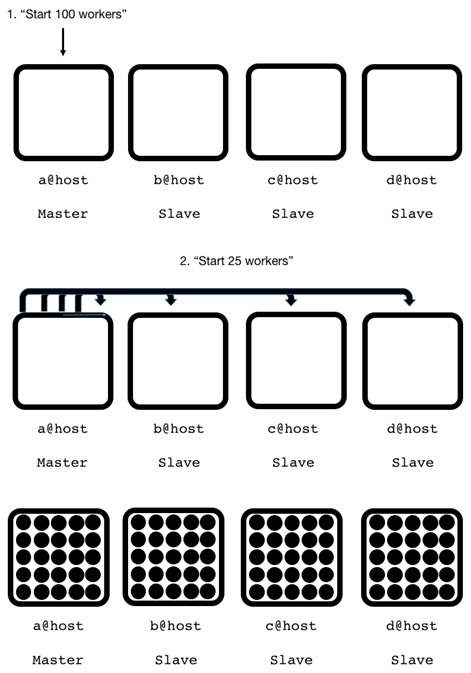
\includegraphics[width=0.8\linewidth]{8_1.png}
    \caption{请求数量被分配到集群中可用的节点上}
    \label{fig:8_1}
\end{figure}


一旦每个节点上的所有工作进程都完成了,结果将被发送到主节点。

\begin{figure}[!ht]
    \centering
    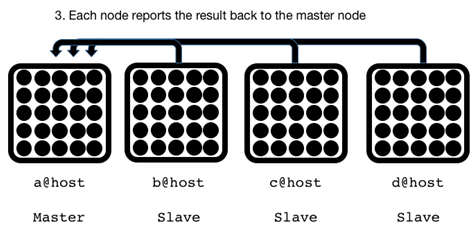
\includegraphics[width=0.8\linewidth]{8_2.png}
    \caption{一旦一个节点收到所有其工作进程的结果,该节点将向主节点报告}
    \label{fig:8_2}
\end{figure}

主节点将汇总并报告结果:

\begin{code}{}  \begin{minted}[linenos]{elixir}
Total workers    : 1000
Successful reqs  : 1000
Failed res       : 0 
Average (msecs)  : 3103.478963 
Longest (msecs)  : 5883.235
Shortest (msecs) : 25.061
\end{minted}
\end{code}

当我计划编写一个分布式应用程序时,我总是先从非分布式版本开始,以保持事情稍微简单一些。一旦你完成了非分布式部分的工作,你可以开始添加分布式层。直接跳入构建一个从一开始就考虑分布式的应用程序通常会出错。

这就是我们在本章中开发Blitzy时采取的方法。实际上,我们将从基础开始:

\begin{enumerate}
\def\labelenumi{\arabic{enumi}.}

\item  构建非并发版本
\item  构建并发版本
\item  构建可以在两个虚拟机实例上运行的分布式版本
\item  构建可以在连接到网络的两台不同机器上运行的分布式版本
\end{enumerate}

\subsection{开始混乱吧!}

给项目起个好名字:

\texttt{\% mix new blitzy}让我们引入一些依赖项,如果我们有预知未来的能力,我们会知道要在\texttt{mix.exs} 中包括这些依赖:

\begin{code}{为 Blitzy 设置依赖项(mix.exs)}

\begin{minted}[linenos]{elixir}
defmodule Blitzy.Mixfile do
  use Mix.Project

  def project do
    [app: :blitzy, version: "0.0.1", elixir: "~> 1.1-rc1", deps: deps]
  end

  def application do
    [
      mod: {Blitzy, []},
      # 3
      applications: [:logger, :httpoison, :timex]
    ]
  end

  defp deps do
    [
      # 1
      {:httpoison, "~> 0.9.0"},
      # 2
      {:timex, "~> 3.0"},
      {:tzdata, "~> 0.1.8", override: true}
    ]
  end
end

# 1 HTTPoison 是一个 HTTP 客户端
# 2 Timex 是一个日期/时间库
# 3 添加必要的应用程序
\end{minted}
% \label{lst:id}
\end{code}



如果你想知道\texttt{\{:tzdata, "~> 0.1.8", override: true\}}是什么意思:之所以需要这样设置是因为新版本的\texttt{tzdata} 不适用于 escripts。Escripts将在本章后面解释。
最后,不要忘记在\texttt{application/0} 中添加正确的条目。


\begin{note}{始终阅读 README!}
  除非我阅读了库的相应 README 中给出的安装说明,否则我不会知道在\texttt{application/0}中包括正确的条目。
  如果不这样做,通常会导致令人困惑的错误。
\end{note}


\subsection{实现工作进程}

我们从工作进程开始。工作进程获取网页并计算请求所用的时间。创建
\texttt{lib/blitzy/worker.ex}。

\begin{code}{实现工作进程(lib/blitzy/worker.ex)}

\begin{minted}[linenos]{elixir}
defmodule Blitzy.Worker do
  use Timex
  require Logger

  def start(url) do
    {timestamp, response} = Duration.measure(fn -> HTTPoison.get(url) end)
    handle_response({Duration.to_milliseconds(timestamp), response})
  end

  defp handle_response({msecs, {:ok, %HTTPoison.Response{status_code: code}}})
       when code >= 200 and code <= 304 do
    Logger.info("worker [#{node}-#{inspect(self)}] completed in #{msecs} msecs")
    {:ok, msecs}
  end

  defp handle_response({_msecs, {:error, reason}}) do
    Logger.info("worker [#{node}-#{inspect(self)}] error due to #{inspect(reason)}")
    {:error, reason}
  end

  defp handle_response({_msecs, _}) do
    Logger.info("worker [#{node}-#{inspect(self)}] errored out")
    {:error, :unknown}
  end
end
\end{minted}
% \label{lst:id}
\end{code}

start 函数接受一个 \texttt{url} 和一个可选的
\texttt{func}。\texttt{func}
是一个用于发出 HTTP
请求的函数。通过这种方式指定一个可选函数,我们可以自由地用另一个 HTTP
客户端替换实现,比如 \emph{HTTPotion}。

例如,我们可以选择使用 HTTPotion 的
\texttt{HTTPotion.get/1} 来代替,就像这样:

\texttt{Blitzy.Worker.start("http://www.bieberfever.com", \&HTTPotion.get/1)}

然后在 \texttt{Time.measure/1} 的主体内调用 HTTP
请求函数。请注意稍微不同的语法:\texttt{func.(url)}
而不是
\texttt{func(url)}。这里的点很重要,因为我们需要告诉
Elixir \texttt{func}
指向另一个函数,而不是那个函数本身。

\texttt{Time.measure/1} 是
\texttt{Timex}
中的一个方便的函数,用于测量函数完成所需的时间。一旦该函数完成,\texttt{Time.measure/1}
就会返回一个包含所用时间和该函数返回值的元组。请注意,所有测量都以毫秒为单位。

从 \texttt{Time.measure/1} 返回的元组然后传递给
\texttt{handle\_response/1}。在这里,

我们期望我们传入 \texttt{start/2}
的任何函数都给我们返回一个包含以下格式之一的元组:

\begin{enumerate}
	\item \mintinline{elixir}|{:ok, \%\{status_code: code\}}|
  \item \mintinline{elixir}|{:error, reason}|
\end{enumerate}

除了获得成功响应外,我们还检查状态代码是否在 200 到 304
的状态代码之间。如果我们遇到错误响应,我们返回一个标记为
\texttt{:error}
的元组以及错误原因。最后,我们处理最后一个情况,即处理所有其他情况。

\subsection{运行工作进程}

让我们尝试运行工作进程:

\begin{code}{}
\begin{minted}[linenos]{elixir}
iex(1) > Blitzy.Worker.start("http://www.bieberfever.com")
{:ok, 2458.665}
\end{minted}
% \label{lst:id}
\end{code}

太棒了!访问 Justin Bieber的粉丝网站大约需要2.4秒。
注意,这也是你等待返回结果所需的时间。那么我们如何同时执行比如说,\emph{一千个}并发请求呢?
使用\texttt{spawn}/\texttt{spawn\_link}!

虽然这可以工作,但我们也需要一种方法来聚合工作进程的返回结果,例如计算所有成功请求的平均所用时间。
我们可以将调用进程作为参数传递给\texttt{Blitzy.Worker.start}函数,并在结果可用时向调用进程发送消息。
反过来,调用进程必须等待来自一千个工作进程的消息。

以下是我们可能如何实现这一点的快速草图。我们引入一个
\texttt{Blitzy.Caller} 模块:

\begin{code}{从工作进程聚合结果的草图}

\begin{minted}[linenos]{elixir}
defmodule Blitzy.Caller do
  def start(n_workers, url) do
    me = self

    1..n_workers
    |> Enum.map(fn _ -> spawn(fn -> Blitzy.Worker.start(url, me) end) end)
    |> Enum.map(fn _ ->
      receive do
        x -> x
      end
    end)
  end
end
\end{minted}
% \label{lst:id}
\end{code}

调用模块接收两个参数。第一个是要创建的工作进程数量,然后是要进行负载测试的
URL。上面的代码可能不太直观,所以让我们一点一点地解释它。

我们首先在 \texttt{me}中保存对调用进程的引用。
为什么?那是因为如果我们在\texttt{spawn} 中使用 \texttt{self}而不是 \texttt{me},
那么 \texttt{self}将指的是新生成的进程,而\emph{不是}调用进程!不信请看:

\begin{code}{}\begin{minted}[linenos]{elixir}
iex(1) > self
# PID<0.159.0>

iex(2) > spawn(fn -> IO.inspect(self) end)
# PID<0.162.0>
\end{minted}
% \label{lst:id}
\end{code}

接下来,我们生成 \texttt{n\_workers}数量的工作进程。

\begin{code}{}\begin{minted}[linenos]{elixir}
1..n_workers
|> Enum.map(fn _ -> spawn(fn -> Blitzy.Worker.start(url, me) end) end)
\end{minted}
% \label{lst:id}
\end{code}

上述结果是一个工作进程 PID 的列表。我们希望 PID将结果发送给调用进程(在下一节中将更多介绍),因此我们等待相同数量的消息:

\begin{code}{}
\begin{minted}[linenos]{elixir}
worker_pids
|> Enum.map(fn _ ->
  receive do
    x -> x
  end
end)
\end{minted}
% \label{lst:id}
\end{code}

我们只需要对 \texttt{Blitzy.Worker.start/1}做一点小修改:

\begin{code}{修改工作进程,以便它可以将其结果发送给调用进程 (lib/worker.ex)}

\begin{minted}[linenos]{elixir}
defmodule Blitzy.Worker do
  # 1
  def start(url, caller, func \\ &HTTPoison.get/1) do
    {timestamp, response} = Duration.measure(fn -> func.(url) end)

    caller
    |> send({self,
     handle_response(
       # 2
       {Duration.to_milliseconds(timestamp), response}
     )})
  end
end

# 1: 添加一个调用者参数
# 2: 无论何时计算出结果,都将结果发送给调用进程
\end{minted}
% \label{lst:id}
\end{code}

上述修改使得 \texttt{Blitzy.Worker}
进程能够将其结果发送给调用进程。

如果这听起来有些混乱,让你有点头痛,那你并不孤单。虽然说实话这并不\emph{那么}难,同时启动一堆任务并等待每个生成的工作进程的结果不应该太难,尤其是因为这是一个常见的用例。幸运的是,这时候\emph{任务}就派上用场了。

\section{任务简介}

任务是 Elixir中执行单一计算的抽象。
这种计算通常简单且自包含,不需要与其他进程进行通信/协调。
为了更好地理解任务如何简化上述场景。

我们可以通过调用 \texttt{Task.async/1}创建一个异步任务:

\begin{code}{}\begin{minted}[linenos]{elixir}
iex > task = Task.async(fn -> Blitzy.Worker.start("http://www.bieberfever.com") end)
\end{minted}
% \label{lst:id}
\end{code}

我们得到的是一个 \texttt{Task} 结构体:

\begin{code}{}\begin{minted}[linenos]{elixir}
%Task{pid: #PID<0.154.0>, ref: #Reference<0.0.3.67>}
\end{minted}
% \label{lst:id}
\end{code}

此时,任务正在后台异步执行。为了从任务中获取值,我们需要调用
\texttt{Task.await/1}:

\begin{code}{创建十个任务,每个任务运行一个 Blitzy 工作进程}

\begin{minted}[linenos]{elixir}
iex > Task.await(task)
{:ok, 3362.655}
\end{minted}
% \label{lst:id}
\end{code}

如果任务仍在计算中会发生什么呢?调用者进程将被阻塞,直到任务完成。让我们试一试:

\begin{code}{}
\begin{minted}[linenos]{elixir}
iex > worker_fun = fn -> Blitzy.Worker.start("http://www.bieberfever.com") end
# Function<20.54118792/0 in :erl_eval.expr/5>
iex > tasks = 1..10 |> Enum.map(fn _ -> Task.async(worker_fun) end)
\end{minted}
% \label{lst:id}
\end{code}

返回结果是十个 \texttt{Task} 结构体的列表

\begin{code}{}
\begin{minted}[linenos]{elixir}
[%Task{pid: #PID<0.184.0>, ref: #Reference<0.0.3.1071>},
 %Task{pid: #PID<0.185.0>, ref: #Reference<0.0.3.1072>},
 %Task{pid: #PID<0.186.0>, ref: #Reference<0.0.3.1073>},
 %Task{pid: #PID<0.187.0>, ref: #Reference<0.0.3.1074>},
 %Task{pid: #PID<0.188.0>, ref: #Reference<0.0.3.1075>},
 %Task{pid: #PID<0.189.0>, ref: #Reference<0.0.3.1076>},
 %Task{pid: #PID<0.190.0>, ref: #Reference<0.0.3.1077>},
 %Task{pid: #PID<0.191.0>, ref: #Reference<0.0.3.1078>},
 %Task{pid: #PID<0.192.0>, ref: #Reference<0.0.3.1079>},
 %Task{pid: #PID<0.193.0>, ref: #Reference<0.0.3.1080>}]
\end{minted}
% \label{lst:id}
\end{code}

现在有十个异步工作进程访问该网站。为了获取结果:

\begin{code}{}\begin{minted}[linenos]{elixir}
iex > result = tasks |> Enum.map(&Task.await(&1))
\end{minted}
% \label{lst:id}
\end{code}

根据您的网络连接情况,Shell进程可能会被阻塞一段时间,之后您会得到类似以下的结果:

\begin{code}{}
\begin{minted}[linenos]{elixir}
[
  ok: 95.023,
  ok: 159.591,
  ok: 190.345,
  ok: 126.191,
  ok: 125.554,
  ok: 109.059,
  ok: 139.883,
  ok: 125.009,
  ok: 101.94,
  ok: 124.955
]
\end{minted}
% \label{lst:id}
\end{code}

这不是很棒吗?我们不仅可以创建异步进程来创建我们的工作进程,而且我们还有一种简单的方法来收集它们的结果。

请系好安全带,因为接下来会更精彩!不需要经历传递调用者的 pid和设置接收块的麻烦。
有了任务,这一切都会被很好地处理。

在 \texttt{lib/blitzy.ex} 中,创建一个\texttt{run/2} 函数来创建和等待工作任务:


\begin{code}{一个方便的函数,用于在任务中运行 Blitzy工作进程(lib/blitzy.ex)}

\begin{minted}[linenos]{elixir}
defmodule Blitzy do
  def run(n_workers, url) when n_workers > 0 do
    worker_fun = fn -> Blitzy.Worker.start(url) end

    1..n_workers
    |> Enum.map(fn _ -> Task.async(worker_fun) end)
    |> Enum.map(&Task.await(&1))
  end
end
\end{minted}
% \label{lst:id}
\end{code}

您现在可以简单地调用 \texttt{Blitzy.run/2}
并以列表形式获取结果:

\begin{code}{}
\begin{minted}[linenos]{elixir}
iex > Blitzy.run(10, "http://www.bieberfever.com")

[
  ok: 71.408,
  ok: 69.315,
  ok: 72.661,
  ok: 67.062,
  ok: 74.63,
  ok: 65.557,
  ok: 201.591,
  ok: 78.879,
  ok: 115.75,
  ok: 66.681
]
\end{minted}
% \label{lst:id}
\end{code}

但有一个小问题。观察当我们将工人数量增加到\emph{一千}时会发生什么:

\begin{code}{}
\begin{minted}[linenos]{elixir}
iex > Blitzy.run(1000, "http://www.bieberfever.com")
\end{minted}
% \label{lst:id}
\end{code}

这会导致:

\begin{code}{当任务超时时出现的错误消息}

\begin{minted}[linenos]{elixir}
(exit) exited in: Task.await(%Task{pid: #PID<0.231.0>, ref: #Reference<0.0.3.1201>}, 5000)
** (EXIT) time out
(elixir) lib/task.ex:274: Task.await/2
(elixir) lib/enum.ex:1043: anonymous fn/3 in Enum.map/2
(elixir) lib/enum.ex:1385: Enum."-reduce/3-lists^foldl/2-0-"/3
(elixir) lib/enum.ex:1043: Enum.map/2
\end{minted}
% \label{lst:id}
\end{code}

问题在于 \texttt{Task.await/2}
默认在\emph{五}秒后超时。我们可以通过给
\texttt{Task.await/2} 提供
\texttt{:infinity} 作为超时值来轻松解决这个问题:

\begin{code}{让任务永远等待 (lib/blitzy.ex)}

\begin{minted}[linenos]{elixir}
defmodule Blitzy do
  def run(n_workers, url) when n_workers > 0 do
    worker_fun = fn -> Blitzy.Worker.start(url) end

    1..n_workers
    |> Enum.map(fn _ -> Task.async(worker_fun) end)
    # 1
    |> Enum.map(&Task.await(&1, :infinity))
  end
end

# 1: 让 Task.await/2 永远等待。
\end{minted}
% \label{lst:id}
\end{code}


在这种情况下指定无限不是问题,因为如果服务器响应时间过长,HTTP
客户端将超时,因此我们愿意将此决定委托给 HTTP 客户端,而不是任务。

最后,我们需要计算平均耗时。在 \texttt{lib/blitzy.ex}中,\texttt{parse\_results/1}负责计算一些简单的统计数据,并将结果格式化为人类友好的格式:

\begin{code}{计算工作器的简单统计信息 (lib/blitzy.ex)}

\begin{minted}[linenos]{elixir}
defmodule Blitzy do
  # ...

  defp parse_results(results) do
    {successes, _failures} =
      Results
      # 1
      |> Enum.partition(fn x ->
        case x do
          {:ok, _} -> true
          _ -> false
        end
      end)

    total_workers = Enum.count(results)
    total_success = Enum.count(successes)
    total_failure = total_workers - total_success

    data = successes |> Enum.map(fn {:ok, time} -> time end)
    average_time = average(data)
    longest_time = Enum.max(data)
    shortest_time = Enum.min(data)

    IO.puts("""
    总工作器数    : #{total_workers}
    成功请求数  : #{total_success}
    失败响应数  : #{total_failure}
    平均时长 (毫秒) : #{average_time}
    最长时长 (毫秒) : #{longest_time}
    最短时长 (毫秒) : #{shortest_time}
    """)
  end

  defp average(list) do
    sum = Enum.sum(list)

    if sum > 0 do
      sum / Enum.count(list)
    else
      0
    end
  end
end

# 1 Enum.partition/2
\end{minted}
\label{lst:compute_simple_statistics}
\end{code}

这部分最有趣的是使用 \texttt{Enum.partition/2}函数。
这个函数接收一个集合和一个谓词函数,并且结果是两个集合。第一个集合包含所有应用谓词函数后返回真值的元素。第二个集合包含被拒绝的元素。在我们的案例中,由于成功的请求看起来像\mintinline{elixir}|{:ok, _}|,而不成功的请求看起来像\mintinline{elixir}|{:error, _}|,我们可以在\mintinline{elixir}|{:ok, _}| 上进行模式匹配。

\section{接下来到分布式!}

我们稍后会再回到 Blitzy。让我们学习如何在 Elixir 中构建一个集群!Erlang
虚拟机的一个杀手级特性是分布式。也就是说,有多个 Erlang
运行时互相通信的能力。当然,你可能也可以在其他语言和平台上做到这一点,但大多数会让你对计算机和人类整体失去信心。

\subsection{位置透明性}

Elixir/Erlang集群中的进程是位置透明的。
这意味着在单个节点上的进程之间发送消息和在不同节点的进程之间发送消息一样容易,只要你知道接收进程的进程ID。

\begin{figure}[!ht]
    \centering
    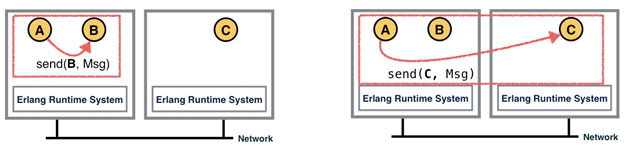
\includegraphics[width=0.8\linewidth]{8_3.png}
    \caption{位置透明性意味着向同一节点上的进程发送消息和向远程节点上的进程发送消息基本没有区别}
    \label{fig:8_3}
\end{figure}



这使得跨节点的进程通信变得非常容易,因为从开发者的角度来看,基本上没有区别。


\subsection{一个 Elixir 节点}

一个节点是运行着 Erlang
虚拟机并被赋予特定名称的系统。名称被表示为一个原子,例如
\texttt{:justin@bieber.com},很像一个电子邮件地址。名称有两种形式,\emph{短}
和 \emph{长}。使用短名称假设所有节点都位于同一 IP
域中。通常,这更容易设置,并且将是我们在本章中坚持使用的。

 \subsection{ 创建集群}

创建集群的第一步是启动一个分布式模式的 Erlang
系统,为此,您必须给它一个名称。在一个新的终端窗口中,启动
\texttt{iex},但这次给它一个短名称
(\texttt{--sname NAME}):

\begin{code}{}
\begin{minted}[linenos]{elixir}
$ iex --sname barry
iex(barry@imac)>
\end{minted}
% \label{lst:id}
\end{code}

注意你的 \texttt{iex}
提示现在有了短名称和本地机器的主机名。要获取本地机器的节点名称,调用
\texttt{Kernel.node/0} 就可以了:

\begin{code}{}
\begin{minted}[linenos]{elixir}
iex(barry@imac)> node
:barry@imac
\end{minted}
% \label{lst:id}
\end{code}

或者,\texttt{Node.self/0} 给你相同的结果,但我更喜欢
\texttt{node}
因为它更短。现在,在两个其他独立的终端窗口中,重复这个过程,但给它们每一个不同的名称:

启动第二个节点:

\begin{code}{}
\begin{minted}[linenos]{elixir}
$ iex --sname robin
iex(robin@imac)>
\end{minted}
% \label{lst:id}
\end{code}

接着是第三个:

\begin{code}{}
\begin{minted}[linenos]{elixir}
$ iex --sname maurice
iex(maurice@imac)>
\end{minted}
% \label{lst:id}
\end{code}

此时,节点仍处于隔离状态 - 它们不知道彼此的存在。

节点必须有唯一的名称!

如果您启动了一个已经被注册的名称的节点,虚拟机将会出现问题。由此可知,您不能混合使用长名称和短名称。

~

\subsection{连接节点}

转到 \texttt{barry} 节点,并使用\texttt{Node.connect/1} 连接到\texttt{robin}:

\begin{code}{}
\begin{minted}[linenos]{elixir}
iex(barry@imac)> Node.connect(:robin@imac)
true
\end{minted}
% \label{lst:id}
\end{code}

\texttt{Node.connect/1} 如果连接成功则返回true。要列出所有 \texttt{barry} 连接的节点,使用\texttt{Node.list/0}:

\begin{code}{}
\begin{minted}[linenos]{elixir}
iex(barry@imac)> Node.list
[:robin@imac]
\end{minted}
% \label{lst:id}
\end{code}

注意 \texttt{Node.list/1}不会列出当前节点,只列出它连接的节点。
现在,转到\texttt{robin} 节点,再次运行\texttt{Node.list/0}:

\begin{code}{}
\begin{minted}[linenos]{elixir}
iex(robin@imac)> Node.list
[:barry@imac]
\end{minted}
% \label{lst:id}
\end{code}

这里没有惊喜。连接 \texttt{barry} 到\texttt{robin} 意味着建立了双向连接。
现在从\texttt{robin},让我们连接到\texttt{maurice}:

\begin{code}{}
\begin{minted}[linenos]{elixir}
iex(robin@imac)> Node.connect(:maurice@imac)
true
\end{minted}
% \label{lst:id}
\end{code}

现在,让我们检查 \texttt{robin} 连接的节点:

\begin{code}{}
\begin{minted}[linenos]{elixir}
iex(robin@imac)> Node.list
[:barry@imac, :maurice@imac]
\end{minted}
% \label{lst:id}
\end{code}

让我们回到 \texttt{barry}。我们没有在\texttt{barry} 上显式运行\texttt{Node.connect(:maurice@imac)}。所以我们应该看到什么呢?

\begin{code}{}
\begin{minted}[linenos]{elixir}
iex(barry@imac)> Node.list
[:robin@imac, :maurice@imac]
\end{minted}
% \label{lst:id}
\end{code}

\subsection{节点连接是传递性的}

太棒了!节点连接是 \emph{传递性的}。这意味着尽管我们没有必要显式地将\texttt{barry} 连接到\texttt{maurice},
但这是因为\texttt{barry} 连接到\texttt{robin},而 \texttt{robin}连接到 \texttt{maurice},
因此 \texttt{barry}连接到了\texttt{maurice}。

\begin{figure}[!ht]
    \centering
    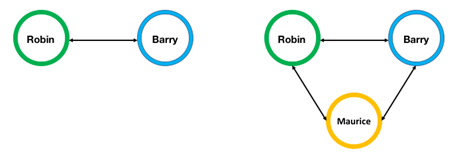
\includegraphics[width=0.8\linewidth]{8_4.png}
    \caption{将一个节点连接到另一个节点会自动将新节点链接到集群中的所有其他节点}
    \label{fig:8_4}
\end{figure}


断开节点会将其从集群的\emph{所有}成员中断开。如果调用了\texttt{Node.disconnect/1}或由于网络中断导致节点死亡,节点可能会断开连接。

\section{远程执行函数}
现在我们知道了如何将节点连接到集群中,让我们做一些有用的事情。首先,关闭所有之前打开的\texttt{iex}会话,因为我们将重新从头开始创建我们的集群。

不过在此之前,转到 \texttt{lib/worker.ex} 并对\texttt{start/3} 函数进行一行添加:

\begin{code}{向 \texttt{lib/worker.ex}中添加一行以打印当前节点}
\begin{minted}[linenos]{elixir}
defmodule Blitzy.Worker do
  def start(url, func \\ &HTTPoison.get/1) do 
      IO.puts "Running on #node-#{node}"             #1 
      {timestamp, response} = Duration.measure(fn -> func.(url) end) 
      handle_response({Duration. Duration.to_milliseconds (timestamp), response}) 
    end
    # ... same as beforeend

#1 打印当前节点
\end{minted}
% \label{lst:id}
\end{code}

这次,转到 \texttt{blitzy}的目录,在\emph{三个}不同的终端中操作。在第一个终端:

\texttt{\% iex --sname barry -S mix}

在第二个终端:

\texttt{\% iex --sname robin -S mix}

最后,在第三个终端:

\texttt{\% iex --sname maurice -S mix}

接下来,我们将所有节点连接在一起。例如,从\texttt{maurice} 节点:

\begin{code}{}
\begin{minted}[linenos]{elixir}
iex(maurice@imac)> Node.connect(:barry@imac)
true

iex(maurice@imac)> Node.connect(:robin@imac)
true

iex(maurice@imac)> Node.list
[:barry@imac, :robin@imac]
\end{minted}
% \label{lst:id}
\end{code}

现在有趣的部分来了。我们现在将在所有三个节点上运行\texttt{Blitzy.Worker.start}。
稍微思考一下,因为这太棒了。
请注意,接下来的命令将在\texttt{maurice}节点上执行。
虽然你可以在任何节点上执行,但某些输出会有所不同。

首先,我们将集群中的每个成员(包括当前节点)的所有引用存储到\texttt{cluster} 中:

\begin{code}{}
\begin{minted}[linenos]{elixir}
iex(maurice@imac)>  cluster = [node | Node.list]
[:maurice@imac, :barry@imac, :robin@imac]
\end{minted}
% \label{lst:id}
\end{code}

然后,我们可以使用 \texttt{:rpc.multicall}函数在所有三个节点上运行\texttt{Blitzy.Worker.start/1}:

\begin{code}{}
\begin{minted}[linenos]{elixir}
  iex(maurice@imac)> :rpc.multicall(cluster, Blitzy.Worker, :start, ["http://www.bieberfever.com"]) 
  "Running on #node-maurice@imac" 
  "Running on #node-robin@imac"
  "Running on #node-barry@imac"
\end{minted}
% \label{lst:id}
\end{code}

返回结果看起来是这样的:

\mintinline{elixir}|{[ok: 2166.561, ok: 3175.567, ok: 2959.726], []}|

事实上,你甚至不需要指定 \texttt{cluster}:

\begin{code}{}
\begin{minted}[linenos]{elixir}
  iex(maurice@imac)> :rpc.multicall(Blitzy.Worker, :start, ["http://www.bieberfever.com"]) 
  "Running on #node-maurice@imac" 
  "Running on #node-barry@imac" 
  "Running on #node-robin@imac"
  {[ok: 1858.212, ok: 737.108, ok: 1038.707], []}
  此材料可能受版权保护。
\end{minted}
% \label{lst:id}
\end{code}

注意,返回值是一个包含两个元素的元组。所有成功的调用都被捕获在第一个元素中,而第二个参数给出了不良(无法到达)节点的列表。

那么,我们如何在多个节点上执行多个\texttt{Worker},同时能够聚合结果并在之后展示它们呢?
我们在实现\texttt{Blitzy.run/2} 时使用\texttt{Task.async/1} 和\texttt{Task.await/2} 解决了这个问题。

\begin{code}{}
\begin{minted}[linenos]{elixir}
iex(maurice@imac)> :rpc.multicall(Blitzy, :run, [5, "http://www.bieberfever.com"], 
:infinity)
\end{minted}
% \label{lst:id}
\end{code}

返回结果是三个列表,每个列表有五个元素。

\begin{code}{}
\begin{minted}[linenos]{elixir}
{[
   [ok: 92.76, ok: 71.179, ok: 138.284, ok: 78.159, ok: 139.742],
   [ok: 120.909, ok: 75.775, ok: 146.515, ok: 86.986, ok: 129.492],
   [ok: 147.873, ok: 171.228, ok: 114.596, ok: 120.745, ok: 130.114]
 ], []}
\end{minted}
% \label{lst:id}
\end{code}

Erlang 的RPC文档中还有许多有趣的函数,例如\texttt{:rpc.pmap/3} 和\texttt{parallel\_eval/1},我鼓励你稍后试验它们。
现在,我们将注意力重新转回到Blitzy。

\section{使 Blitzy 分布式}

我们将创建一个简单的配置文件,主节点将使用它来连接到集群的节点。
打开\texttt{config/config.exs} 并填写以下内容:

\begin{code}{整个集群的配置文件(config/config.exs)}

\begin{minted}[linenos]{elixir}
use Mix.Config

config :blitzy, master_node: :"a@127.0.0.1"

config :blitzy, slave_nodes: [:"b@127.0.0.1", :"c@127.0.0.1", :"d@127.0.0.1"]
\end{minted}
% \label{lst:id}
\end{code}

\subsection{创建命令行界面}

Blitzy是一个命令行程序。因此,让我们为它构建一个命令行界面。创建一个名为\texttt{cli.ex} 的新文件并将其放在\texttt{lib} 中。
我们希望这样调用\texttt{Blitzy}:

\texttt{./blitzy -n [requests] [url]}

\texttt{[requests]}是一个指定要创建\texttt{Worker}数量的整数,而 \texttt{[url]}是一个指定端点的字符串。
如果用户未能提供正确的格式,则还应显示帮助消息。在Elixir 中,很容易将这些连接起来。

首先,转到 \texttt{mix.exs} 并修改\texttt{project/0}。创建一个名为\texttt{escript} 的条目,并填写如下:

\begin{code}{将 escript添加到项目函数中以确定命令行程序的主入口点(mix.exs)}
\begin{minted}[linenos]{elixir}
defmodule Blitzy.Mixfile do
  def project do
    [
      app: :blitzy,
      version: "0.0.1",
      elixir: "~> 1.1",
      # 1
      escript: [main_module: Blitzy.CLI],
      deps: deps
    ]
  end
end
\end{minted}
\label{lst:escript}
\end{code}

这指向 \texttt{mix} 当我们调用\texttt{mix escript.build} 生成\texttt{Blitzy} 命令行程序时的正确模块。
由\texttt{main\_module} 指向的模块应该有一个\texttt{main/1} 函数。
让我们提供它和一些其他函数:

\subsection{使用 OptionParser 解析输入参数}

\begin{code}{使用 OptionParser 处理输入参数 (lib/cli.ex)}

\begin{minted}[linenos]{elixir}
use Mix.Config
defmodule Blitzy.CLI do
  require Logger

  def main(args) do
    args
    |> parse_args
    |> process_options
  end

  defp parse_args(args) do
    OptionParser.parse(args, aliases: [n: :requests],
    strict: [requests: :integer])
  end

  defp process_options(options, nodes) do
    case options do
      {[requests: n], [url], []} ->
        # 执行操作

      _ ->
        do_help
    end
  end
end
\end{minted}
% \label{lst:id}
\end{code}

大多数 Elixir的命令行程序都有相同的一般结构,即接收参数,解析它们,并处理它们。多亏了管道操作符,我们可以这样表示:

\begin{code}{}
\begin{minted}[linenos]{elixir}
args
|> parse_args
|> process_options
\end{minted}
% \label{lst:id}
\end{code}

\texttt{args} 是一个参数的标记化列表。例如,给定

\begin{code}{}
\begin{minted}[linenos]{elixir}
% ./blitzy -n 100 http://www.bieberfever.com
\end{minted}
% \label{lst:id}
\end{code}

那么 \texttt{args} 是:

\begin{code}{}
\begin{minted}[linenos]{elixir}
["-n", "100", "http://www.bieberfever.com"]
\end{minted}
% \label{lst:id}
\end{code}

这个列表然后被传递给 \texttt{parse\_args/1},这是\texttt{OptionParser.parse/2}的一个简单封装。
\texttt{OptionParser.parse/2}完成了大部分繁重的工作。

它接受一个参数列表并返回解析后的值、剩余的参数和无效选项。让我们看看如何解读这个:

\begin{code}{}
\begin{minted}[linenos]{elixir}
OptionParser.parse(args,
  aliases: [n: :requests],
  strict: [requests: :integer]
)
\end{minted}
% \label{lst:id}
\end{code}

首先,我们将 \texttt{--requests} 别名为\texttt{n}。
这是指定开关的简写方式。\texttt{OptionParser}期望所有开关都以 \texttt{--<switch>} 开始,单字符开关\texttt{-<switch>}应该适当地别名。
例如,\texttt{OptionParser}将这样的命令视为无效:

\begin{code}{}
\begin{minted}[linenos]{elixir}
iex > OptionParser.parse(["-n", "100"])
{[], [], [{"-n", "100"}]}
\end{minted}
% \label{lst:id}
\end{code}

你可以告诉它是无效的,因为是第三个列表被填充了。
另一方面,如果你为开关添加了双破折号(即长格式),那么\texttt{OptionParser} 就会接受它:

\begin{code}{}
\begin{minted}[linenos]{elixir}
iex(d@127.0.0.1)12> OptionParser.parse(["--n", "100"])
{[n: "100"], [], []}
\end{minted}
% \label{lst:id}
\end{code}

我们还可以对开关值的类型进行断言。\texttt{-n}的值必须是整数。
因此,我们在上面的代码中的\texttt{strict}选项中指定了这一点。
请再次注意,我们使用的是开关的长名称。

一旦我们完成了参数的解析,我们可以将结果交给\texttt{process\_options/1}。
在这个函数中,我们利用了\texttt{OptionParser.parse/2}返回的是一个有三个元素的元组,每个元素都是一个列表。

\begin{code}{通过模式匹配,我们可以轻松声明程序期望的参数格式 (lib/cli.ex)}

\begin{minted}[linenos]{elixir}
defp process_options(options) do
  case options do
    {[requests: n], [url], []} -> #1
      # 稍后实现。
    _ ->
      do_help
  end
end

#1 模式匹配我们期望的确切格式
\end{minted}
% \label{lst:id}
\end{code}

我们还模式匹配了程序所期望的\emph{确切}格式。仔细审视一下模式:

\begin{code}{}
\begin{minted}[linenos]{elixir}
{[requests: n], [url], []}
\end{minted}
% \label{lst:id}
\end{code}

你能指出我们对参数所声明的一些属性吗?这是我的:

\begin{enumerate}
\def\labelenumi{\arabic{enumi}.}
\item  \texttt{--requests} 或 \texttt{-n}  包含一个也是整数的单一值。
\item  还有一个 URL。
\item  没有无效的参数。这是通过第三个元素中的空列表指定的。
\end{enumerate}

如果由于某种原因参数无效,那么我们希望调用 \texttt{do\_help}函数来呈现一个友好的信息:


\begin{code}{当用户错误使用参数时添加一个简单的帮助函数 (lib/cli.ex)}

\begin{minted}[linenos]{elixir}
defp do_help do
  IO.puts("""
  使用方法:
  blitzy -n [请求次数] [url]

  选项:
  -n, [--requests]      # 请求次数

  示例:
  ./blitzy -n 100 http://www.bieberfever.com
  """)

  System.halt(0)
end
\end{minted}
% \label{lst:id}
\end{code}

目前,当参数有效时不会发生任何事情。现在让我们填补缺失的部分。

\subsection{连接到节点}

我们之前在 \texttt{config/config.exs}中创建了一个配置,指定了主节点和从节点。
我们如何从我们的应用程序中访问这个配置呢?非常简单:

\begin{code}{}
\begin{minted}[linenos]{elixir}
iex(1) > Application.get_env(:blitzy, :master_node)
:"a@127.0.0.1"

iex(2) > Application.get_env(:blitzy, :slave_nodes)
[:"b@127.0.0.1", :"c@127.0.0.1", :"d@127.0.0.1"]
\end{minted}
% \label{lst:id}
\end{code}

注意,节点 \texttt{b}、\texttt{c} 和\texttt{d}需要在分布式模式下启动并使用匹配的名称,
然后才能执行命令\texttt{(./blitzy -n 100 http://www.bieberfever.com)}。
我们需要修改\texttt{lib/cli.ex} 中的\texttt{main/1} 函数:

\begin{code}{修改 main 以从配置文件中读取 (lib/cli.ex)}

\begin{minted}[linenos]{elixir}
defmodule Blitzy.CLI do
  def main(args) do
    # 1
    Application.get_env(:blitzy, :master_node)
    # 1
    |> Node.start()

    # 2
    Application.get_env(:blitzy, :slave_nodes)
    # 2
    |> Enum.each(&Node.connect(&1))

    args
    |> parse_args
    # 3
    |> process_options([node | Node.list()])
  end
end

# 1 在分布式模式下启动主节点
# 2 连接到从节点
\end{minted}
% \label{lst:id}
\end{code}


我们从 \texttt{config/config.exs}中读取配置。
首先,我们在分布式模式下启动主节点,并将其命名为\texttt{a@127.0.0.1}。
接下来,我们连接到从节点。然后,我们将整个集群的列表传递给\texttt{process\_options/2},现在它接受两个参数(之前只接受一个)。
接下来,让我们修改它:

\begin{code}{这个函数现在接受集群中的节点列表,并将其传递给 do\_requests}

\begin{minted}[linenos]{elixir}
defmodule Blitzy.CLI do
  # ...

  defp process_options(options, nodes) do
    case options do
      {[requests: n], [url], []} ->
        # 1
        do_requests(n, url, nodes)

      _ ->
        do_help
    end
  end
end

# 1 节点列表被传递给 do\_requests/3
\end{minted}
% \label{lst:id}
\end{code}

节点列表被传递到 \texttt{do\_requests/3}
函数,这是主要的工作函数:

\begin{code}{}
\begin{minted}[linenos]{elixir}
defmodule Blitzy.CLI do
  # ...

  defp do_requests(n_requests, url, nodes) do
    Logger.info("Pummelling #{url} with #{n_requests} requests")

    # 1
    total_nodes = Enum.count(nodes)
    # 1
    req_per_node = div(n_requests, total_nodes)

    nodes
    |> Enum.flat_map(fn node ->
      1..req_per_node
      |> Enum.map(fn _ ->
        Task.Supervisor.async({Blitzy.TasksSupervisor, node}, Blitzy.Worker, :start, [url])
      end)
    end)
    |> Enum.map(&Task.await(&1, :infinity))
    |> parse_results
  end
end

# 1 计算每个节点要生成的工作器数量
\end{minted}
% \label{lst:id}
\end{code}

以上代码相对简洁,但不用担心!我们很快就会再次讨论它。现在,让我们暂时绕道去看看任务\emph{监督器}。

\subsection{使用 Tasks.Supervisor 监督任务}

我们不希望一个 \texttt{Task}
的崩溃导致整个应用程序崩溃。这在我们可能生成\emph{成千上万}个(甚至更多!)\texttt{Task}
时尤其重要。到现在为止,你应该知道答案是将
\texttt{Task} 置于监督之下。

幸运的是,Elixir 配备了一个专门的 \texttt{Task}
监督器,恰当地称为
\texttt{Task.Supervisor}。这个监督器是一个
\texttt{:simple\_one\_for\_one} 监督器,

其中所有被监督的 \texttt{Task}
都是临时的(在崩溃时不会重启)。为了使用
\texttt{Task.Supervisor},我们需要创建
\texttt{lib/supervisor.ex}:

\begin{figure}[!ht]
    \centering
    \includegraphics[width=0.8\linewidth]{8_5.png}
    \caption{Blitzy 的监督树}
    \label{fig:8_5}
\end{figure}

 

\begin{code}{设置顶级监督树 (lib/supervisor.ex)}

\begin{minted}[linenos]{elixir}
defmodule Blitzy.Supervisor do
  use Supervisor

  def start_link(:ok) do
    Supervisor.start_link(__MODULE__, :ok)
  end

  def init(:ok) do
    children = [
      supervisor(Task.Supervisor, [[name: Blitzy.TasksSupervisor]])
    ]

    supervise(children, strategy: :one_for_one)
  end
end
\end{minted}
% \label{lst:id}
\end{code}

我们创建了一个顶级监督器(\texttt{Blitzy.Supervisor}),它监督一个我们命名为
\texttt{Blitzy.TasksSupervisor} 的
\texttt{Task.Supervisor}。现在,我们需要在应用程序启动时启动
\texttt{Blitzy.Supervisor}。这是
\texttt{lib/blitzy.ex}:

\begin{code}{}
\begin{minted}[linenos]{elixir}
defmodule Blitzy do
  use Application

  def start(_type, _args) do
    Blitzy.Supervisor.start_link(:ok)
  end
end
\end{minted}
% \label{lst:id}
\end{code}

\texttt{start/2} 函数只是启动顶级监督器,然后启动其余的监督树。

\subsection{使用任务监督器}

让我们仔细看看这段代码,因为它展示了我们如何利用\texttt{任务监督器(Task.Supervisor)}在所有节点上分配工作负载,
以及如何使用\texttt{任务等待(Task.await/2)} 来检索结果:

\begin{code}{}
\begin{minted}[linenos]{elixir}
nodes
|> Enum.flat_map(fn node ->
  1..req_per_node
  |> Enum.map(fn _ ->
    Task.Supervisor.async({Blitzy.TasksSupervisor, node}, Blitzy.Worker, :start, [url])
  end)
end)
|> Enum.map(&Task.await(&1, :infinity))
|> parse_results
\end{minted}
% \label{lst:id}
\end{code}

这可能是最复杂的一行:

\begin{code}{}
\begin{minted}[linenos]{elixir}
Task.Supervisor.async({Blitzy.TasksSupervisor, node}, Blitzy.Worker, :start, [url])
\end{minted}
% \label{lst:id}
\end{code}

这与启动一个 \texttt{任务(Task)} 类似:

\begin{code}{}
\begin{minted}[linenos]{elixir}
Task.async(Blitzy.Worker, :start, ["http://www.bieberfever.com"])
\end{minted}
% \label{lst:id}
\end{code}

然而,有几个关键的不同。首先,从\texttt{任务监督器(Task.Supervisor)}启动任务意味着它受到监督!
其次,仔细看看第一个参数。我们传入了一个包含模块名\emph{和}节点的元组。
换句话说,我们在远程告诉每个节点的\texttt{Blitzy.TasksSupervisor} 生成工作器。这太棒了!
\texttt{任务监督器异步(Task.Supervisor.async/3)}返回的与 \texttt{任务异步(Task.async/3)} 相同,一个\texttt{任务(Task)} 结构:

\begin{code}{}
\begin{minted}[linenos]{elixir}
%Task{pid: #PID<0.154.0>, ref: #Reference<0.0.3.67>}
\end{minted}
% \label{lst:id}
\end{code}

因此,我们可以调用 \texttt{任务等待(Task.await/2)}
来等待每个工作器返回的结果。现在我们已经解决了难点,我们可以更好地理解这段代码的目的。给定一个节点,我们生成
\texttt{req\_per\_node} 数量的工作器:

\begin{code}{}
\begin{minted}[linenos]{elixir}
1..req_per_node
|> Enum.map(fn _ ->
  Task.Supervisor.async({Blitzy.TasksSupervisor, node}, Blitzy.Worker, :start, [url])
end)
\end{minted}
% \label{lst:id}
\end{code}

为了在所有节点上执行此操作,我们必须以某种方式\emph{映射}通过所有节点。
我们\emph{可以}使用\texttt{Enum.map/2}:

\begin{code}{}
\begin{minted}[linenos]{elixir}
nodes
|> Enum.map(fn node ->
  1..req_per_node
  |> Enum.map(fn _ ->
    Task.Supervisor.async({Blitzy.TasksSupervisor, node}, Blitzy.Worker, :start, [url])
  end)
end)
\end{minted}
% \label{lst:id}
\end{code}

然而,这个结果将是一个嵌套列表的 \texttt{任务(Task)}结构,因为内部 \texttt{Enum.map/2}的结果是任务结构的列表。
相反,我们想要的是\texttt{Enum.flat\_map/2},它看起来像这样,它接受任意嵌套的列表,扁平化列表然后对扁平列表中的每个元素应用函数。
下图说明了这一点:

\begin{figure}[!ht]
    \centering
    \includegraphics[width=0.8\linewidth]{8_7.png}
    \caption{使用 flatmap 扁平化任务结构列表,然后将每个任务结构映射到Blitzy 任务监督器}
    \label{fig:8_7}
\end{figure}

图\ref{fig:8_7}这里,我们使用 flatmap来扁平化任务结构的列表,然后将每个任务结构映射到 Blitzy 任务监督器

这是代码:

\begin{code}{}
\begin{minted}[linenos]{elixir}
nodes
|> Enum.flat_map(fn node ->
  1..req_per_node
  |> Enum.map(fn _ ->
    Task.Supervisor.async({Blitzy.TasksSupervisor, node}, Blitzy.Worker, :start, [url])
  end)
end)
\end{minted}
% \label{lst:id}
\end{code}

由于现在我们有了一个\emph{扁平化}的任务结构列表,我们可以交给\texttt{任务等待(Task.await/2)}:

\begin{code}{}
\begin{minted}[linenos]{elixir}
nodes
|> Enum.flat_map(fn node ->
  nil
  # 一个任务结构的列表
end)

# 由于 flat map,一个任务结构的列表
|> Enum.map(&Task.await(&1, :infinity))
|> parse_results
\end{minted}
% \label{lst:id}
\end{code}

\texttt{任务等待(Task.await/2)}

本质上完成了从所有节点收集结果到主节点的工作。完成后,我们像之前一样将列表交给\texttt{解析结果(parse\_results/1)}。

\subsection{创建二进制文件与 \texttt{mix escript.build}}

差不多了!最后一步是生成二进制文件。在项目目录中,运行以下\texttt{mix} 命令:

\begin{code}{构建可执行文件}

\begin{minted}[linenos]{elixir}
% mix escript.build
编译 lib/supervisor.ex
编译 lib/cli.ex
生成 blitzy 应用
用 MIX_ENV=dev 生成 escript blitzy
\end{minted}
% \label{lst:id}
\end{code}

最后一行告诉你 \texttt{blitzy}
二进制文件已经创建。如果你列出目录中的所有文件,你会找到
\texttt{blitzy}:

\begin{code}{运行 mix escript.build 后生成 blitzy 二进制文件}
\begin{minted}[linenos]{elixir}
% ls
README.md     blitzy        deps          lib           mix.lock      test
_build        config        erl_crash.dump mix.exs       priv
\end{minted}
% \label{lst:id}
\end{code}

\subsection{运行 Blitzy!}

终于到了!在我们启动二进制文件之前,我们需要先启动\emph{三个}其他节点。记住,这些是从节点。在三个不同的终端里,启动从节点:

\begin{code}{运行 mix escript.build 后生成 blitzy 二进制文件}
  \begin{minted}[linenos]{elixir}
% iex --name b@127.0.0.1 -S mix
% iex --name c@127.0.0.1 -S mix
% iex --name d@127.0.0.1 -S mix
\end{minted}
% \label{lst:id}
\end{code}

现在,我们可以运行 \texttt{blitzy}
了!在另一个终端中,运行 \texttt{blitzy} 命令:

\texttt{\% ./blitzy -n 10000 http://www.bieberfever.com}你会看到所有四个终端都显示出类似的信息:

\texttt{10:34:17.702 [info]  worker [b@127.0.0.1-\#PID<0.2584.0>] completed in 58585.746 msecs}。
下面是在我的机器上的一个例子:

\begin{figure}[!ht]
    \centering
    \includegraphics[width=0.8\linewidth]{8_7a.png}
    \caption{在我的机器上运行 Blitzy}
    \label{fig:8_7a}
\end{figure}


最后,当一切完成后,结果将会在你启动 \texttt{./blitzy}
命令的终端上报告:

\texttt{总工作者数    : 10000}
\texttt{成功请求    : 9795}
\texttt{失败响应     : 205}
\texttt{平均时间 (毫秒) : 31670.991222460456}
\texttt{最长时间 (毫秒) : 58585.746``最短时间 (毫秒) : 3141.722}

\section{总结}

在这章里,我们得到了关于分布式 Elixir能提供什么的广泛概览。
下面是快速回顾:

\begin{itemize}
\item  Elixir 和 Erlang VM 提供的用于构建分布式系统的内置函数
\item  实现一个展示负载均衡的分布式应用
\item  学习如何使用任务进行短暂计算
\item  实现一个命令行应用程序
\end{itemize}

在下一章中,我们将继续探索分布式的冒险。我们将探讨分布式和容错是如何相辅相成的。

\chapter{分布式和容错性}\label{chapt:distribution}

本章内容包括:

\begin{itemize}

\item
  实现分布式和容错性应用程序
\item
  Cookies和安全
\item
  在局域网(LAN)中连接节点
\end{itemize}

在上一章中,我们了解了Elixir中分布式的基础知识。特别是,我们现在知道如何建立一个集群。我们还研究了\emph{任务(Tasks)},这是一种抽象,它可以让我们轻松编写短暂的计算。

接下来我们要探索的概念是分布式环境下的容错性。为此,我们将构建一个应用程序,演示当一个节点宕机时,如何由另一个节点自动接管其工作。更进一步,该应用程序还将演示当一个优先级更高的之前宕机的节点重新加入集群时,如何让当前的节点让出控制权。换句话说,我们将构建一个展示分布式Elixir的\emph{故障转移(failover)}和\emph{接管(takeover)}能力的应用程序。

\section{分布式容错性}

故障转移发生在运行应用程序的节点宕机时,该应用程序会在另一个节点上自动重启,给定一定的超时期限。接管发生在一个节点的优先级(在列表中定义)高于当前运行节点时,导致优先级较低的节点停止,并在优先级更高的节点上重启应用程序。在编程中,至少当你看到故障转移和接管实际发生时,它们非常酷。

Chucky Chuck Norris 事实应用程序概述

我们要构建的应用程序将会故意保持简单,因为主要目标是学习如何将您的OTP应用程序连接起来,使其具有容错性,使用故障转移和接管。我们将构建\emph{Chucky},一个分布式且具有容错性的Chuck
Norris``事实''应用程序。这是Chucky的一个示例运行:

\texttt{iex(1)> Chucky.fact}
\texttt{"Chuck Norris的键盘没有Ctrl键,因为没有什么能控制Chuck Norris。"}

\texttt{iex(2)> Chucky.fact}
\texttt{"Chuck Norris声明的所有数组都是无限大小的,因为Chuck Norris不受限制。"}
\section{构建Chucky}

Chucky是一个简单的OTP应用程序。应用程序的核心在于一个GenServer。我们将首先构建它,然后实现Application行为。最后,我们将亲自看到如何将所有内容连接起来,以利用故障转移和接管。

\subsection{实现服务器}

您知道该怎么做:

\texttt{\% mix new chucky} 接下来,创建
\texttt{lib/server.ex}:

代码 9.1 实现主Chucky服务器(lib/server.ex)

\texttt{defmodule Chucky.Server do}
\texttt{use GenServer}

\texttt{\#\#\#\#\#\#\#}
\texttt{\# API \#}
\texttt{\#\#\#\#\#\#\#}

\texttt{def start\_link do}
\texttt{GenServer.start\_link(\_\_MODULE\_\_, [], [name: \{:global, \_\_MODULE\_\_\}]) \#1}
\texttt{end}

\texttt{def fact do}
\texttt{GenServer.call(\{:global, \_\_MODULE\_\_\}, :fact)                        \#2}
\texttt{end}

\texttt{\#\#\#\#\#\#\#\#\#\#\#\#\#}
\texttt{\# Callbacks \#}
\texttt{\#\#\#\#\#\#\#\#\#\#\#\#\#}

\texttt{def init([]) do}
\texttt{:random.seed(:os.timestamp)}
\texttt{facts = "facts.txt"}
\texttt{|> File.read!}
\texttt{|> String.split("\\n")}

\mintinline{elixir}|{:ok, facts}| \texttt{end}

\texttt{def handle\_call(:fact, \_from, facts) do}
\texttt{random\_fact = facts}
\texttt{|> Enum.shuffle}
\texttt{|> List.first}

\mintinline{elixir}|{:reply, random_fact, facts}|
\texttt{end} \texttt{end} \#1
在集群内全局注册GenServer

\#2 对全局注册的GenServer进行调用(和casts)需要额外的 :global

这里的大部分代码应该不难理解,尽管在 `

Chucky.Server.start\_link/0\texttt{和}Chucky.Server.fact/1\texttt{中使用的}:global\texttt{是新的。在}Chucky.Server.start\_link/0\texttt{,我们使用}\{:global,
\textbf{MODULE}\}\texttt{注册了模块的名称。这样做的效果是将}Chucky.Server\texttt{注册到}global\_name\_server`
进程上。每次节点启动时,都会启动此进程。这意味着没有单个``特殊''的节点来跟踪名称表。相反,每个节点都将有名称表的副本。

由于我们已经全局注册了此模块,调用(和casts)也必须以
\texttt{:global}为前缀。因此,我们不是写

\texttt{def fact do}
\texttt{GenServer.call(\_\_MODULE\_\_, :fact)``end}
我们这样做:

\texttt{def fact do}
\texttt{GenServer.call(\{:global, \_\_MODULE\_\_\}, :fact)``end}
\texttt{init/1} 回调读取一个名为
\texttt{facts.txt}的文件,基于换行符将其分割,并将
\texttt{Chucky.Server} 的状态初始化为``事实''的列表。将
\texttt{facts.txt}
存储在项目根目录中。您可以从项目的GitHub仓库获取文件副本。

\texttt{handle\_call/3}
回调简单地从其状态(``事实''的列表)中随机选择一个条目,并返回它。

\subsection{实现应用程序行为}

接下来,我们将实现作为应用程序入口点的应用程序行为。此外,我们可以从
\texttt{Chucky.start/2}中创建一个显式的监督器。这是通过导入
\texttt{Supervisor.Spec} 来完成的,它暴露了
\texttt{worker/2}
函数(创建子进程规范),我们可以将其传递给
\texttt{Supervisor.start\_link} 函数,以结束
\texttt{start/2}。创建
\texttt{lib/chucky.ex}:

\begin{code}{实现应用程序行为(lib/chucky.ex)}
\begin{minted}[linenos]{elixir}
defmodule Chucky do
  use Application
  require Logger

  def start(type, _args) do
    import Supervisor.Spec

    children = [
      worker(Chucky.Server, [])
    ]

    case type do
      :normal ->
        Logger.info("Application is started on #{node}")

      {:takeover, old_node} ->
        Logger.info("#{node} is taking over #{old_node}")

      {:failover, old_node} ->
        Logger.info("#{old_node} is failing over to #{node}")
    end

    opts = [strategy: :one_for_one, name: {:global, Chucky.Supervisor}]
    Supervisor.start_link(children, opts)
  end

  def fact do
    Chucky.Server.fact()
  end
end
\end{minted}
% \label{lst:id}
\end{code}

这是一个简单的监督器,监督 \texttt{Chucky.Server}。就像
\texttt{Chucky.Server}一样,
\texttt{Chucky.Supervisor} 也是全局注册的,因此使用
\texttt{:global}注册。

\subsection{应用类型参数}

请注意,我们在此使用了 \texttt{start/2} 的
\texttt{type}
参数,这是我们通常会忽略的。对于非分布式应用程序,\texttt{type}
的值通常是 \texttt{:normal}。但当我们开始处理
takeover(接管)和 failover(故障转移)时,情况就变得有趣了。

如果您查阅 Erlang 文档中 \texttt{type}
参数所期望的数据类型,您将看到这样的内容:

\begin{figure}[!ht]
    \centering
    \includegraphics[width=0.8\linewidth]{9_0.png}
    \caption{Erlang 文档中\texttt{type}参数的数据类型说明}
    \label{fig:9_0}
\end{figure}

这正是我们在上述代码中匹配的三种情况。当应用程序以分布式模式启动时,对于
\mintinline{elixir}|{:takeover, node}| 和
\mintinline{elixir}|{:failover, node}| 的模式匹配将成功。

不详细介绍(下一节将详述),当一个节点因为要接管另一个节点(因为它具有更高优先级)而启动时,\mintinline{elixir}|{:takeover, node}|
中的 \texttt{node} 就是被接管的节点。

类似地,当一个节点因为另一个节点死亡而启动时,\mintinline{elixir}|{:failover, node}|
中的 \texttt{node}
就是死亡的那个节点。到目前为止,我们还没有编写任何特定于故障转移或接管的代码。我们接下来将处理这个。

\section{Chucky 中故障转移和接管概述}

在进入具体细节之前,让我们谈谈集群的
\emph{行为}。在这个例子中,我们将配置一个由三个节点组成的集群。为了方便参考,以及大多是因为作者缺乏想象力,我们将节点命名为
\texttt{a@<host>}、\texttt{b@<host>}
和 \texttt{c@<host>},其中
\texttt{<host>} 是您的主机名。本节剩余部分,我将仅用
\texttt{a}、\texttt{b} 和
\texttt{c} 来指代所有节点。

节点 \texttt{a} 将是主节点,而
\texttt{b} 和 \texttt{c}
将是从节点。在接下来的图表中,带有绿色环的节点是主节点。其余的是从节点。

节点启动的 \emph{顺序} 很重要。在这种情况下,\texttt{a}
首先启动,其次是 \texttt{b} 和
\texttt{c}。当所有节点都启动后,集群就完全初始化了。换句话说,只有
\texttt{a}、\texttt{b} 和
\texttt{c} 初始化后,集群才会变得可用。

所有三个节点都已编译
Chucky(这是一个重要的细节)。然而,当集群启动时,只有 \emph{一个}
应用程序启动,它在主节点上启动(惊喜!)。这意味着,虽然请求可以从集群中的任何节点发出,但只有主节点会回应该请求:


\begin{figure}[!ht]
    \centering
    \includegraphics[width=0.8\linewidth]{9_1.png}
    \caption{所有请求都由 a\@host 处理,无论哪个节点接收到请求}
    \label{fig:9_1}
\end{figure}


现在让情况变得有趣。当 \texttt{a}
失败时,其余节点将在一段时间后检测到 \texttt{a}
已失败。然后它将在其中一个从节点上启动应用程序。在这种情况下,是
\texttt{b}:

\begin{figure}[!ht]
    \centering
    \includegraphics[width=0.8\linewidth]{9_2.png}
    \caption{假设 a\@host 失败。在 5 秒内,一个故障转移节点将接管(见下图)}
    \label{fig:9_2}
\end{figure}

\begin{figure}[!ht]
    \centering
    \includegraphics[width=0.8\linewidth]{9_3.png}
    \caption{b\@host 在检测到 a@host 失败后自动接管}
    \label{fig:9_3}
\end{figure}


图 9.3 b@host 在检测到 a@host 失败后自动接管

如果 \texttt{b} 失败了呢?那么
\texttt{c}
就是下一个启动应用程序的节点。到目前为止,我们介绍的都是故障转移情况。

现在,考虑一些更有趣的事情。当 \texttt{a}
重启时会发生什么?由于 \texttt{a}
是主节点,它在其余节点中具有 \emph{最高优先级}。因此,它将发起
\emph{接管}:

\begin{figure}[!ht]
    \centering
    \includegraphics[width=0.8\linewidth]{9_4.png}
    \caption{一旦 a\@host 回来,它将发起接管}
    \label{fig:9_4}
\end{figure}


无论哪个从节点正在运行应用程序,它都将退出,并将控制权让给主节点。这有多棒?现在,我们可以看到如何在
Chucky 中实现故障转移和接管策略。


\subsection{故障转移和接管配置}

在本节中,我们将看到为您的分布式应用程序配置故障转移和接管所需的步骤。

\subsubsection{步骤1:确定机器的主机名}

第一步是找出您要使用的机器的主机名。例如,在我的Mac OSX上:

\texttt{\% hostname –s}
\texttt{manticore} 步骤2:为每个节点创建配置文件

\subsubsection{步骤2:为每个节点创建配置文件}

为了简单起见,在\texttt{config} 目录中创建这三个文件:

\begin{enumerate}
	\item \texttt{a.config}
  \item \texttt{b.config}
  \item \texttt{c.config}
\end{enumerate}

注意它们被命名为\texttt{<节点名称>.config}。虽然您可以自由命名任何文件名,但我建议您坚持使用此约定,因为每个文件将包含节点特定的配置细节。

\subsubsection{步骤3:填写每个节点的配置文件}

每个节点的配置文件结构看起来有点复杂,但我们稍后会更仔细地检查一下。现在,在
\texttt{config/a.config}中输入这个:


\begin{code}{a@host的配置 (config/a.config)}
\begin{minted}[linenos]{elixir}
[{kernel, 
    [{distributed, [{chucky, 5000, [a@manticore, {b@manticore, c@manticore}]}]}, 
     {sync_nodes_mandatory, [b@manticore, c@manticore]}, 
     {sync_nodes_timeout, 30000}
    ]}].
\end{minted}
\label{lst:a_host_config}
\end{code}


这代表配置单个节点的故障转移/接管所需的配置。让我们分解一下。我们从最复杂的部分开始,\texttt{distributed} 配置参数:

\texttt{[\{distributed, [\{chucky, 5000, [a@manticore, \{b@manticore, c@manticore\}]\}]\}]}
\texttt{chucky} 当然是应用程序名称。
\texttt{5000}
代表节点被认为宕机之前的超时毫秒数,应用程序在下一个最高优先级的节点中重启。

\texttt{[a@manticore, \{b@manticore, c@manticore\}]}
列出了优先级顺序的节点。在这个例子中, \texttt{a}
是首位,其次是 \texttt{b} 或
\texttt{c}。在元组中定义的节点之间没有优先级。例如,考虑以下条目:

\texttt{[a@manticore, \{b@manticore, c@manticore\}, d@manticore]}
在这种情况下,最高优先级是 \texttt{a},然后是\texttt{b/c},接着是 \texttt{d}。
\begin{enumerate}
\item  \texttt{sync\_nodes\_mandatory}:\emph{必须}在\texttt{sync\_nodes\_timeout}指定的时间内启动的节点列表
\item  \texttt{sync\_nodes\_optional}:\emph{可以}在\texttt{sync\_nodes\_timeout}指定的时间内启动的节点列表。(注意,我们没有在这个应用程序中使用此选项)
\item \texttt{sync\_nodes\_timeout}:等待其他节点启动的时间(以毫秒为单位)
\end{enumerate}

\texttt{sync\_nodes\_mandatory} 和
\texttt{sync\_nodes\_optional}
的区别是什么?顾名思义,正在启动的节点将在
\texttt{sync\_nodes\_timeout} 设置的超时限制内等待所有
\texttt{sync\_nodes\_mandatory}
中的节点启动。如果有一个未能启动,则节点会终止自身。对于
\texttt{sync\_nodes\_optional}
则不是那么严格。节点只是等待直到超时过去,并且如果任何节点没有启动,\emph{不会}自我终止。

配置从节点

对于剩下的节点,配置\emph{几乎}相同,除了
\texttt{sync\_nodes\_mandatory}
条目。事实上,保持其余配置不变是\emph{非常}重要的。例如,有不一致的
\texttt{sync\_nodes\_timeout}
值会导致群集的不确定行为。

这是 \texttt{b}的配置:

\begin{code}{b@host的配置 (config/b.config)}
  \begin{minted}[linenos]{elixir}
\begin{code}{}      \begin{minted}[linenos]{elixir}
      [{kernel, [{distributed, [{chucky, 5000, [a@manticore, {b@manticore, c@manticore}]}]},
        {sync_nodes_mandatory, [a@manticore, c@manticore]},
        {sync_nodes_timeout, 30000}]}].
\end{minted}
  \label{lst:b_host_config}
  \end{code}

这是 \texttt{c}的配置:

\begin{code}{c@host的配置 (config/c.config)}
  \begin{minted}[linenos]{elixir}
[{kernel,
        [{distributed,
          [{chucky, 5000,
            [a@manticore, {b@manticore, c@manticore}]}]},
         {sync_nodes_mandatory, [a@manticore, b@manticore]},
         {sync_nodes_timeout, 30000}]}].
\end{minted}
  \label{lst:c_host_config}
  \end{code}


\subsubsection{步骤4:在所有节点上编译Chucky}

应用程序应该在其所在的机器上编译。 \texttt{Chucky}的编译非常简单:

\texttt{\% mix compile}
再次提醒,在\emph{每台机器}上都要这样做。

\subsubsection{步骤5:启动分布式应用程序}

打开三个不同的终端。在每个终端上,运行这些命令:

对于\texttt{a}:

\texttt{\% iex --sname a -pa \_build/dev/lib/chucky/ebin --app chucky --erl "-config config/a.config"}
接下来,对于\texttt{b}:

\texttt{\% iex --sname b -pa \_build/dev/lib/chucky/ebin --app chucky --erl "-config config/b.config"}
最后,对于\texttt{c}:

\texttt{\% iex --sname c -pa \_build/dev/lib/chucky/ebin --app chucky --erl "-config config/c.config"}
上述咒语虽然有点神秘,但仍可解释: ~ -
\texttt{--sname <name>}:启动一个分布式节点,并为其分配\emph{短名称}。~
-
\texttt{-pa <path>}:将给定路径\emph{前置}到Erlang代码路径。这个路径指向从Chucky运行
-
\texttt{mix compile}后生成的BEAM文件。(\emph{附加}版本是\texttt{-pz}。)~~
-
\texttt{--app <application>}:启动应用程序及其依赖项。
-
\texttt{--erl <switches>}:传递给Erlang的开关。在我们的示例中,
- \texttt{-config config/c.config}用于配置OTP应用程序。

\section{故障转移和接管实战}

经过这么多努力,让我们看看实际效果吧!你会注意到,当你启动
\texttt{a}(甚至
\texttt{b})时,直到启动 \texttt{c}
才会发生事情。在每个终端中运行 \texttt{Chucky.fact}:

\begin{code}{Chucky 可以从集群中的任何节点访问}

\begin{minted}[linenos]{elixir}
23:10:54.465 [info]  Application is started on a@manticore
iex(a@manticore)1> Chucky.fact
"Chuck Norris doesn't read, he just stares the book down until it tells him what he wants."

iex(b@manticore)1> Chucky.fact
"Chuck Norris can use his fist as his SSH key. His foot is his GPG key."

iex(c@manticore)1> Chucky.fact
"Chuck Norris never wet his bed as a child. The bed wet itself out of fear."
\end{minted}
% \label{lst:id}
\end{code}

虽然 \emph{看起来}应用程序在每个单独的节点上运行,我们可以轻松地说服自己这不是这种情况。
注意在第一个终端,消息\texttt{Application is started on a@manticore} 在\texttt{a} 上打印出来,但在其他节点上没有。

还有另一种方法可以告诉我们当前节点上运行了哪些应用程序。
使用\texttt{Application.started\_applications/1},我们可以清楚地看到\texttt{Chucky} 在 \texttt{a} 上运行:

\begin{code}{Application.started\_applications/0 显示 a@host 上的 Chucky}

\begin{minted}[linenos]{elixir}
iex(a@manticore)1> Application.started_applications
[{:chucky, 'chucky', '0.0.1'}, {:logger, 'logger', '1.1.1'},
 {:iex, 'iex', '1.1.1'}, {:elixir, 'elixir', '1.1.1'},
 {:compiler, 'ERTS CXC 138 10', '6.0.1'}, {:stdlib, 'ERTS CXC 138 10', '2.6'}, {:kernel, 'ERTS CXC 138 10', '4.1'}]
\end{minted}
% \label{lst:id}
\end{code}

然而,\texttt{Chucky} \emph{没有} 在
\texttt{b} 和 \texttt{c}
上运行。这里只显示了 \texttt{b}
的输出,因为两个节点的输出是相同的:

\begin{code}{Chucky 没有在 b@host 和 c@host(未显示)上运行}

\begin{minted}[linenos]{elixir}
iex(b@manticore)1> Application.started_applications
[{:logger, 'logger', '1.1.1'}, {:iex, 'iex', '1.1.1'},
 {:elixir, 'elixir', '1.1.1'}, {:compiler, 'ERTS CXC 138 10', '6.0.1'}, {:stdlib, 'ERTS CXC 138 10', '2.6'}, {:kernel, 'ERTS CXC 138 10', '4.1'}]
\end{minted}
% \label{lst:id}
\end{code}

现在,让我们通过退出 \texttt{iex}(按两次 Ctrl +
C)来终止 \texttt{a}。大约5秒钟后,你会注意到
\texttt{Chucky} 现在已经自动在
\texttt{b} 上启动了:

\begin{code}{当 a@host 停止后,b@host 接管}

\begin{minted}[linenos]{elixir}
iex(b@manticore)1>
23:16:42.161 [info]  Application is started on b@manticore
\end{minted}
% \label{lst:id}
\end{code}

这是多么棒的事情!集群中的剩余节点判定 \texttt{a}
不可达并假定其已死亡。因此,\texttt{b} 承担了运行
\texttt{Chucky} 的责任。如果你现在在
\texttt{b} 上运行
\texttt{Application.started\_applications/1},你会看到类似的内容:

代码 9.10 重新运行 Application.started\_applications/0 现在显示 b@host
上的 Chucky

\begin{code}{}
\begin{minted}[linenos]{elixir}
iex(b@manticore)2> Application.started_applications
[{:chucky, 'chucky', '0.0.1'}, {:logger, 'logger', '1.1.1'},
 {:iex, 'iex', '1.1.1'}, {:

elixir, 'elixir', '1.1.1'},
 {:compiler, 'ERTS CXC 138 10', '6.0.1'}, {:stdlib, 'ERTS CXC 138 10', '2.6'}, {:kernel, 'ERTS CXC 138 10', '4.1'}]
\end{minted}
% \label{lst:id}
\end{code}

在 \texttt{c} 上,你可以确信
\texttt{Chucky} 仍在运行:

\begin{code}{通常情况下,仍然可以从 c@host 访问 Chucky}

\begin{minted}[linenos]{elixir}
iex(c@manticore)1> Chucky.fact
"The Bermuda Triangle used to be the Bermuda Square, until Chuck Norris Roundhouse kicked one of the corners off."
\end{minted}
% \label{lst:id}
\end{code}

现在,让我们看看接管实战。当 \texttt{a}重新加入集群时会发生什么?由于 \texttt{a}是集群中优先级最高的节点,\texttt{b} 将让位给\texttt{a}。
换句话说,\texttt{a}将接管 \texttt{b}。再次启动\texttt{a}:

\begin{code}{}
\begin{minted}[linenos]{elixir}
% iex --sname a -pa _build/dev/lib/chucky/ebin --app chucky --erl "-config config/a.config"
\end{minted}
% \label{lst:id}
\end{code}

在 \texttt{a} 中,你会看到类似的内容:

\begin{code}{}
\begin{minted}[linenos]{elixir}
23:23:36.695 [info]  a@manticore is taking over b@manticore
iex(a@manticore)1>
\end{minted}
% \label{lst:id}
\end{code}

在 \texttt{b} 中,你会注意到应用程序已停止:

\begin{code}{当 a@host 重新启动并重新加入集群时,b@host 让位}

\begin{minted}[linenos]{elixir}
iex(b@manticore)3>
23:23:36.707 [info]  Application chucky exited: :stopped
\end{minted}
% \label{lst:id}
\end{code}

当然,\texttt{b} 仍然可以提供一些 Chuck Norris 的事实:

\begin{code}{}
\begin{minted}[linenos]{elixir}
iex(b@manticore)4> Chucky.fact
"It takes Chuck Norris 20 minutes to watch 60 Minutes."
\end{minted}
% \label{lst:id}
\end{code}

就这样!我们已经看到了一整个故障转移和接管周期。在下一节中,我们将看看如何连接同一本地区域网络中的节点。

\section{连接局域网中的节点,Cookie 和安全性}

安全性在 Erlang
设计师思考分布式时并不是一个重要考虑因素。原因是节点将在他们自己的内部/可信网络中使用。因此,事情被保持得相当简单。

为了让两个节点通信,他们需要做的就是共享一个 \emph{cookie}。这个 cookie
是一个通常存储在你的主目录中的纯文本文件:

\begin{code}{}
\begin{minted}[linenos]{bash}
% cat ~/.erlang.cookie
XLVCOLWHHRIXHRRJXVCN
\end{minted}
% \label{lst:id}
\end{code}

当你在同一台机器上启动节点时,你不必担心
cookie,因为所有节点在你的主目录中共享同一个
cookie。然而,一旦你开始连接到其他机器,你将不得不确保这些 cookie
都是相同的。不过,还有另一种选择。你也可以显式地调用
\texttt{Node.set\_cookie/2}。在本节中,我们将看到如何连接到不在同一台机器上,但在同一局域网络中的节点。

\subsection{查询两台机器的IP地址}

首先,我们需要找出两台机器的IP地址。在Linux/Unix系统上,通常使用\texttt{ifconfig}命令。同时,请确保它们都连接到同一个局域网(LAN)。这可能意味着将机器插入同一个路由器/交换机,或者让机器连接到同一个无线接入点。下面是我在其中一台机器上的样例输出:

\begin{code}{我的机器上的ifconfig输出}

\begin{minted}[linenos]{bash}
% ifconfig
lo0: flags=8049<UP,LOOPBACK,RUNNING,MULTICAST> mtu 16384
options=3<RXCSUM,TXCSUM>
inet6 ::1 prefixlen 128
inet 127.0.0.1 netmask 0xff000000
inet6 fe80::1%lo0 prefixlen 64 scopeid 0x1
nd6 options=1<PERFORMNUD>
gif0: flags=8010<POINTOPOINT,MULTICAST> mtu 1280
stf0: flags=0<> mtu 1280
en0: flags=8863<UP,BROADCAST,SMART,RUNNING,SIMPLEX,MULTICAST> mtu 1500
ether 10:93:e9:05:19:da
inet6 fe80::1293:e9ff:fe05:19da%en0 prefixlen 64 scopeid 0x4
inet 192.168.0.100 netmask 0xffffff00 broadcast 192.168.0.255
nd6 options=1<PERFORMNUD>
media: autoselect status: active
\end{minted}
% \label{lst:id}
\end{code}

你应该关注的数字是\texttt{192.168.0.100}。当我在另一台机器上执行相同步骤时,IP地址是\texttt{192.168.0.103}。请注意,我们在这里使用的是IPv4地址。如果你使用IPv6地址,你将需要在接下来的示例中使用IPv6地址。

\subsection{将两个节点连接起来}

让我们试试看。在第一台机器上,启动\texttt{iex},但这次使用长名称(\texttt{--name})标志。同时,在名称后附加\texttt{@<ip-address>}。

\begin{code}{}
\begin{minted}[linenos]{elixir}
% iex --name one@192.168.0.100
Erlang/OTP 18 [erts-7.1] [source] [64-bit] [smp:4:4] [async-threads:10] [hipe] [kernel-poll:false] [dtrace]

Interactive Elixir (0.13.1-dev) - press Ctrl+C to exit (type h() ENTER for help)iex(one@192.168.0.100)1>
\end{minted}
% \label{lst:id}
\end{code}

在第二个节点上执行相同的步骤:

\begin{code}{}
\begin{minted}[linenos]{elixir}
% iex --name two@192.168.0.103
Erlang/OTP 18 [erts-7.1] [source] [64-bit] [smp:4:4] [async-threads:10] [hipe] [kernel-poll:false] [dtrace]

Interactive Elixir (1.1.1) - press Ctrl+C to exit (type h() ENTER for help)iex(two@192.168.0.103)1>
\end{minted}
% \label{lst:id}
\end{code}

现在,让我们尝试将\texttt{one@192.168.0.100}和\texttt{two@192.168.0.103}连接起来:

\begin{code}{}
\begin{minted}[linenos]{elixir}
iex(one@192.168.0.100)1> Node.connect :'two@192.168.0.103'
false
\end{minted}
% \label{lst:id}
\end{code}

等等,为什么呢?在\texttt{two@192.168.0.103}上,你会看到一个类似的错误报告:

\begin{code}{}
\begin{minted}[linenos]{elixir}
=ERROR REPORT==== 25-May-2014::22:32:25 ===
** Connection attempt from disallowed node 'one@192.168.0.100' **
\end{minted}
% \label{lst:id}
\end{code}

发生了什么?原来,我们缺少了一个关键成分------\emph{cookie}。

\subsection{记住Cookie!}

当你在同一台机器上连接节点\emph{并且}没有使用\texttt{--cookie}标志设置任何cookie时,Erlang
VM只是使用存储在你的主目录中生成的cookie:

\begin{code}{}
\begin{minted}[linenos]{bash}
% cat ~/.erlang.cookie
XBYWEVWS

NBAROAXWPTZX%
\end{minted}
% \label{lst:id}
\end{code}

这意味着,如果你在\emph{同一}本地机器上\emph{不使用}
cookie标志连接节点,通常不会遇到任何问题。

然而,在不同的机器上,这就是一个问题。这是因为各个机器上的cookies很可能不同。考虑到这一点,让我们重新开始整个过程。这次,我们为每个节点提供相同的cookie值。或者,你也可以将相同的\texttt{.\~/.erlang-cookie}复制到所有节点上。在本节中,我们使用前一种技术。在第一台机器上:

\begin{code}{}
\begin{minted}[linenos]{elixir}
% iex --name one@192.168.0.100 --cookie monster
Erlang/OTP 18 [erts-7.1] [source] [64-bit] [smp:4:4] [async-threads:10] [hipe] [kernel-poll:false] [dtrace]

Interactive Elixir (1.1.1) - press Ctrl+C to exit (type h() ENTER for help)iex(one@192.168.0.100)1>
\end{minted}
% \label{lst:id}
\end{code}

在第二台机器上,我们确保使用\emph{相同}的cookie值:

\begin{code}{}
\begin{minted}[linenos]{elixir}
% iex --name two@192.168.0.103 --cookie monster
Erlang/OTP 18 [erts-7.1] [source] [64-bit] [smp:4:4] [async-threads:10] [hipe] [kernel-poll:false] [dtrace]

Interactive Elixir (1.1.1) - press Ctrl+C to exit (type h() ENTER for help)iex(two@192.168.0.103)1>
\end{minted}
% \label{lst:id}
\end{code}

让我们再次尝试将\texttt{one@192.168.0.100}连接到\texttt{two@192.168.0.103}:

\begin{code}{}
\begin{minted}[linenos]{elixir}
iex(one@192.168.0.100)1> Node.connect :'two@192.168.0.103'
true
\end{minted}
% \label{lst:id}
\end{code}

太好了!我们已经成功地在局域网上建立了一个Elixir集群。作为一个健康检查,我们也可以做一个\texttt{Node.list/0}。回想一下,这个函数只列出它的邻居,因此不包括当前节点:

\begin{code}{}
\begin{minted}[linenos]{elixir}
iex(one@192.168.0.100)2> Node.list
[:"two@192.168.0.103"]
\end{minted}
% \label{lst:id}
\end{code}

\section{总结}

在一个预期能够承受崩溃的应用程序中实现正确的故障转移(Failover)和接管(Takeover)是绝对必要的。与许多语言和平台不同,故障转移和接管在
OTP 中是内置的。在这一章中,我们继续探索分布式系统。特别地,我们覆盖了:

\begin{itemize}

\item  实现一个展示故障转移和接管的分布式应用程序
\item  配置故障转移和接管
\item  将节点连接到局域网(LAN)
\item  使用 Cookie
\item  一些关于 Chuck Norris 的笑话
\end{itemize}

在接下来的章节和之后的章节中,我们将探讨在 Elixir中的测试。
我们不仅仅覆盖单元测试,还将探索基于属性的测试,并学习如何测试并发程序。


%Part 3
\part{类型规范和测试}\label{part3}

"让它崩溃"的原则并不意味着你可以编写未经测试的代码。在本书的最后一部分,我们将研究使我们的
Elixir 代码更可靠的技术和工具。

我们将研究
Dialyzer,并学习如何用类型规范来捕获我们代码中的错误。然后我们将进入基于属性的测试,学习如何断言我们函数的属性,并学习编写为我们生成测试的代码。

虽然在 Elixir
中编写并发代码肯定更容易,但错误肯定会出现。在最后一章中,我们将研究
Concuerror,这是一个用来寻找并发错误的工具。

\chapter{Dialyzer和类型规范}\label{chapt:dialyzer}

本章内容包括:

\begin{itemize}

\item  什么是Dialyzer以及它是如何工作的
\item  使用Dialyzer发现代码中的不一致
\item  编写类型规范和定义自己的类型
\end{itemize}

根据你的倾向,类型的提及可能会让你欣喜若狂或者退避三舍。作为一种动态类型语言,Elixir免除了你在代码库中大量使用类型的需求,这一点类似于Haskell。有人可能会认为这导致了更快的开发周期。然而,Elixir程序员不应该过于自满。静态类型语言可以在\emph{编译}时捕捉到一整类错误,而动态语言只能在\emph{运行时}捕捉到这些错误。

幸运的是,语言中内置的容错功能试图拯救我们自己。没有这些功能的语言(Ruby,我在看你)将会直接崩溃。然而,我们有责任尽可能地使我们的软件可靠。在本章中,我们将学习如何利用类型来实现这一点。

我们将了解Dialyzer,这是一个与Erlang发行版捆绑在一起的工具。这个强大的工具用于消除某些类别的软件错误。最棒的部分是,你不需要对你的代码做任何特别的处理。

你将了解一些关于Dialyzer背后有趣的理论。这将帮助你解读它的(有时是隐晦的)错误信息。你还将理解为什么Dialyzer不是解决所有类型问题的灵丹妙药。

在本章的最后部分,我们将学习如何通过在代码中添加类型,使Dialyzer更好地寻找错误。在本章结束时,你将学会如何将Dialyzer作为开发工作流的一部分。

Dialyzer的命名者因为这个与电信相关的缩写而值得加薪。Dialyzer代表了Erlang的不一致性分析器。Dialyzer是一个帮助你发现代码中不一致之处的工具。具体是什么类型的不一致呢?以下是一个列表:

\begin{itemize}

\item  类型错误
\item  引发异常的代码
\item  无法满足的条件
\item  冗余代码
\item  竞态条件
\end{itemize}

我们将很快亲自看到Dialyzer是如何发现这些不一致的。在此之前,了解Dialyzer的内部工作原理是有帮助的。

\section{10.1 Dialyzer是如何工作的}

静态语言可以在编译时捕捉潜在的错误。动态语言的本质意味着它们只能在运行时检测到这些错误。Dialyzer试图将静态类型检查器的一些优点带给像Elixir/Erlang这样的动态语言。

Dialyzer的主要目标之一是不干扰现有程序。这意味着不应该期望任何Erlang(和Elixir)程序员重写代码来适应Dialyzer。

这导致了一个非常好的结果:你不需要提供给Dialyzer任何额外的信息,它就能完成它的工作。这并不是说你\emph{不能}这样做。事实上,正如你稍后将看到的,你可以提供额外的类型信息,让Dialyzer在寻找不一致时做得更好。

\section{10.2 成功类型}

Dialyzer使用\emph{成功类型}的概念来收集和推断类型信息。了解Dialyzer

如何工作是值得的。要理解成功类型是什么,我们需要了解一点关于Elixir类型系统的知识。

像Elixir这样的动态语言需要一个比静态类型系统更宽松的类型系统,因为函数可能会接受多种类型的参数。

例如,让我们看看布尔``和''函数。在像Haskell这样的静态语言中,\texttt{and}函数可以这样实现:

\begin{code}{Haskell中的布尔与运算}
  \begin{minted}[linenos]{Haskell}
    and :: Bool -> Bool -> Bool
    and x y | x == True && y == True = True
                | otherwise = False
  \end{minted}
  \label{lst:boolean-in-haskell}
\end{code}

第一行 \texttt{and :: Bool -> Bool -> Bool}是函数的类型参数。
它表明 \texttt{and}是一个接受两个布尔值作为参数并返回一个布尔值的函数。
如果类型检查器看到任何非布尔值作为输入到\texttt{and},你的程序将无法通过编译。Elixir版本会是什么样子呢?

\begin{code}{在Elixir中实现的布尔与运算}
\begin{minted}[linenos]{elixir} 
defmodule MyBoolean do

  def and(true, true) do
    true
  end
  
  def and(false, _) do
    false
  end
  
  def and(_, false) do
    false
  end
  
end
\end{minted}
\label{lst:boolean-in-elixir}
\end{code}

多亏了模式匹配,我们可以将\texttt{and/2} 表示为三个函数子句。
什么是对\texttt{and/2}的有效参数?第一和第二个参数接受\texttt{true}, \texttt{false}和\texttt{\_}, 而返回值都是布尔值。

正如你已经知道的,``\_''意味着``任何东西''。
因此,以下是对\texttt{and/2}的完全合理的调用:

\begin{code}{在Elixir中实现的布尔与运算}
  \begin{minted}[linenos]{elixir} 
    MyBoolean.and(true, true) MyBoolean.and(false, "great success!")
    MyBoolean.and([1, 2, 3], false)
  \end{minted}
\end{code}

Haskell类型检查器不会允许像前面展示的Elixir程序,因为它不允许将``任何东西''作为一种类型。它无法处理这种不确定性。

另一方面,Dialyzer采用了一种不同的类型推断算法,称为成功类型。成功类型非常乐观。它总是假设你的所有函数都被正确使用。
因此,你的代码在被证明有罪之前是无辜的。

成功类型从\emph{过度估计}你的函数的有效输入和输出开始。
所以它从假设你的函数可以接受任何东西并返回任何东西开始。
然而,随着它更好地理解你的代码,它会生成\emph{约束}。
这些约束反过来将限制输入值以及对应的输出。

例如,如果它看到 \texttt{x + y},那么\texttt{x} 和 \texttt{y}肯定是数字。
像 \texttt{is\_atom(z)}这样的守卫也提供了额外的约束。
一旦生成了约束,就是解决它们的时候了,就像解谜一样。
谜题的解答就是函数的成功类型。
相反,如果没有找到解决方案,约束是\emph{不可满足的},你手头就有一个类型违规。

然而,重要的是要意识到,因为Dialyzer总是假设你的代码是正确的,所以它\emph{不}保证你的代码是类型安全的。现在,在你起身离开房间之前,由此产生了一个非常好的属性。如果Dialyzer发现了什么问题,那么它\emph{肯定}是对的。所以Dialyzer的第一课是这样的:

\begin{note}{Dialyzer永远不会出错!}
Dialyzer 在它说你的代码有问题时,始终是正确的。
\end{note}


这就是为什么当Dialyzer表示你的代码有问题时,它是100\%正确的。
更严格的类型检查器从假设你的代码是错误的开始,你的代码必须成功通过类型检查才能允许编译。这也意味着你的代码(或多或少)被保证是类型安全的。

所以再次强调:Dialyzer\emph{不会}(或永远不会)发现所有类型违规。
然而,如果它发现了问题,那么你的代码\emph{肯定}存在问题。
现在我们对成功类型(success typings)的工作方式有了一些背景知识,让我们转向了解Elixir中的类型。

\section{揭示Elixir中的类型,第一部分}

我们一直在使用Elixir,但并没有太多强调确切的类型。在本节和下一节中,我们将稍微更加关注这一点。

从Elixir1.2开始,有一个非常方便的工具在\texttt{iex}中可以打印给定数据类型的信息,称为\texttt{i/1}。
例如,\texttt{"ohai"}和\texttt{'ohai'}之间有什么区别(注意分别使用双引号和单引号)?让我们来找出答案:

\begin{code}{使用i/1揭示Elixir字符串的类型}
\begin{minted}[linenos]{elixir}
iex(1)> i("ohai")
  Term
    "ohai"
  Data type
    BitString
  Byte size
    4
  Description
    This is a string: a UTF-8 encoded binary. It's printed surrounded by
    "double quotes" because all UTF-8 encoded code points in it are printable.
  Raw representation
    <<111, 104, 97, 105>>
  Reference modules
    String, :binary
  Implemented protocols
    Collectable, IEx.Info, Inspect, List.Chars, String.Chars
\end{minted}
% \label{lst:id}
\end{code}

现在让我们对比一下\texttt{'ohai'}:

\begin{code}{使用i/1揭示字符列表的类型}

\begin{minted}[linenos]{elixir}
iex(2)> i('ohei')
  Term
    ~c"ohei"
  Data type
    List
  Description
    This is a list of integers that is printed using the `~c` sigil syntax,
    defined by the `Kernel.sigil_c/2` macro, because all the integers in it
    represent printable ASCII characters. Conventionally, a list of Unicode
    code points is known as a charlist and a list of ASCII characters is a
    subset of it.
  Raw representation
    [111, 104, 101, 105]
  Reference modules
    List
  Implemented protocols
    Collectable, Enumerable, IEx.Info, Inspect, List.Chars, String.Chars
\end{minted}
% \label{lst:id}
\end{code}

下次如果你遇到类型错误并感到困惑,立即使用\texttt{i/1}工具。

\section{开始使用Dialyzer}

Dialyzer可以使用Erlang源代码或调试编译的BEAM字节码。显然,这让我们只能选择后者。这意味着在我们运行Dialyzer之前,必须记得先执行\texttt{mix compile}。

\begin{note}{记得先编译!} 
  
  自从开始使用Dialyzer以来,我已经忘记了多少次这个步骤。幸运的是,一旦我发现了Dialyxir(稍后你会看到),我就不再需要手动编译我的代码了。
  
\end{note}

Dialyzer随Erlang发行版安装,并且存在作为命令行程序:

\begin{code}{}\begin{minted}[linenos]{elixir}
  % dialyzer
      Checking whether the PLT /Users/benjamintan/.dialyzer_plt is up-to-date... 
      dialyzer: Could not find the PLT: /Users/benjamintan/.dialyzer_plt Use the options: 
      --build_plt   to build a new PLT; or 
      --add_to_plt  to add to an existing PLT
      
      For example, use a command like the following: 
         dialyzer --build_plt --apps erts kernel stdlib mnesia Note that building a PLT such as the above may take 20 mins or so 

      If you later need information about other applications, say crypto, you can extend the PLT by the command: 
        dialyzer --add_to_plt --apps crypto
      For applications that are not in Erlang/OTP use an absolute file name.
\end{minted}
% \label{lst:id}
\end{code}

太好了,我们已经确信Dialyzer确实已安装。但是这个\emph{PLT}是什么,Dialyzer正在尝试搜索什么呢?

\subsection{PLT:持久查找表}

PLT代表持久查找表(Persistent Lookup Table)。Dialyzer使用PLT来存储其分析结果。您还可以使用之前构建的PLT作为Dialyzer的起点。这变得很重要,因为任何非平凡的Elixir应用程序可能都会涉及OTP。如果我们对这样的应用程序运行Dialyzer,分析无疑会花费很长时间。

由于OTP库不会改变,我们总是可以构建一个``基础PLT'',只在我们的应用程序上运行Dialyzer,相比之下将会花费更短的时间。这的另一面是,一旦您升级了Erlang和/或Elixir,您必须记得重建PLT。

 \subsection{ Dialyxir(Dialyxir)}

传统上,运行 Dialyzer需要输入相当多的命令。幸好,由于程序员的懒惰,现在有一些库包含了\texttt{mix}任务,使我们的生活更加轻松。
我们将使用的一个库是\emph{Dialyxir}。
Dialyxir 包含了 \texttt{mix}任务,使得在 Elixir 项目中使用 Dialyzer 成为一种乐趣。

Dialyxir可以作为依赖安装(我们稍后会看到),也可以全局安装。我们首先全局安装Dialyxir,以便构建 PLT 表。
这不是绝对必要的,但当你不想将 Dialyxir安装为项目依赖时,这是很有用的:

\begin{code}{}\begin{minted}[linenos]{elixir}
git clone https://github.com/jeremyjh/dialyxir
cd dialyxir
mix archive.build
mix archive.install
\end{minted}
% \label{lst:id}
\end{code}

让我们开始使用 Dialyxir 吧!

\subsection{构建 PLT 表(建立 PLT表)}

如前所述,我们首先需要构建 PLT。令人高兴的是,Dialyxir 有一个 mix任务用于构建 PLT:

\begin{code}{}
\begin{minted}[linenos]{elixir}
% mix dialyzer.plt
\end{minted}
% \label{lst:id}
\end{code}

准备好咖啡,因为这需要一段时间:

\begin{code}{}
\begin{minted}[linenos]{elixir}
Starting PLT Core Build ... this will take awhile
dialyzer --output_plt /Users/benjamintan/.dialyxir_core_18_1.2.0-rc.1.plt --build_plt --apps erts kernel stdlib crypto public_key -r /usr/local/Cellar/elixir/HEAD/bin/../lib/elixir/../eex/ebin /usr/local/Cellar/elixir/HEAD/bin/../lib/elixir/../elixir/ebin /usr/local/Cellar/elixir/HEAD/bin/../lib/elixir/../ex_unit/ebin /usr/local/Cellar/elixir/HEAD/bin/../lib/elixir/../iex/ebin /usr/local/Cellar/elixir/HEAD/bin/../lib/elixir/../mix/ebin
...
cover:compile_beam_directory/1
cover:modules/0
cover:start/0
fprof:analyse/1
fprof:apply/3
fprof:profile/1
httpc:request/5
httpc:set_options/2
inets:start/2
inets:stop/2
leex:file/2
yecc:file/2
Unknown types:
compile:option/0
done in 2m33.16s
done (passed successfully)
\end{minted}
% \label{lst:id}
\end{code}

只要 PLT 构建成功,你就不必担心``未知类型''和其他警告。


\section{10.5 Dialyzer 可以检测的软件差异(Dialyzer能检测的软件问题)}

在本节中,我们将创建一个项目来进行实验。示例项目是一个简单的货币转换器,只能将新加坡元转换为美元。创建项目:

\begin{code}{}\begin{minted}[linenos]{elixir}
% mix new dialyzer_playground
\end{minted}
% \label{lst:id}
\end{code}

打开 \texttt{mix.exs} 并添加 Dialyxir:


\begin{code}{代码 10.4 添加 dialyxir 依赖(mix.exs)}

\begin{minted}[linenos]{elixir}
defmodule DialyzerPlayground.Mixfile do
  # ...

  defp deps do
    [{:dialyxir, "~> 0.3", only: [:dev]}]
  end
end
\end{minted}
% \label{lst:id}
\end{code}

像往常一样,记得运行\texttt{mix deps.get}。现在乐趣开始了!


\subsection{捕捉类型错误(捕获类型错误)}

我们从一个简单的示例开始,演示 Dialyzer 如何捕捉简单的类型错误。创建
\texttt{lib/bug\_1.ex}:

\begin{code}{代码 10.5 Cashy.Bug1有一个类型错误。你能发现吗?(lib/bug\_1.ex)}

\begin{minted}[linenos]{elixir}
defmodule Cashy.Bug1 do

  def convert(:sgd, :usd, amount) do
    {:ok, amount * 0.70}
  end

  def run do
    convert(:sg

d, :usd, :one_million_dollars)
  end
end
\end{minted}
% \label{lst:id}
\end{code}

\texttt{convert/3} 函数接受三个参数。前两个参数\emph{必须} 是原子 \texttt{:sgd} 和\texttt{:usd}。
\texttt{amount}被假定为一个数字,并用来计算从新加坡元到美元的汇率。相当直接的东西。

现在想象一下 \texttt{run/1}函数可能存在于另一个模块中。
不难想象有人错误地使用这个函数,比如将原子作为\texttt{convert/3} 的最后一个参数,而不是数字。

只有当 \texttt{run/1}被执行时,代码的问题才会显现。
否则,这个问题甚至可能不会浮现。值得注意的是,静态类型语言永远不会允许这样的代码。
对我们来说幸运的是,我们有Dialyzer!让我们运行 Dialyzer 看看会发生什么:

\begin{code}{}
\begin{minted}[linenos]{elixir}
% mix dialyzer
\end{minted}
% \label{lst:id}
\end{code}

这是输出:

\begin{code}{}
\begin{minted}[linenos]{elixir}
% mix dialyzer
Compiled lib/bug_1.ex
Generated dialyzer_playground app
...
Proceeding with analysis...
bug_1.ex:7: Function run/0 has no local return
bug_1.ex:8: The call 'Elixir.Cashy.Bug1':convert('sgd','usd','one_million_dollars') will never return since it differs in the 3rd argument from the success typing arguments: ('sgd','usd',number())
done in 0m1.00s
done (warnings were emitted)
\end{minted}
% \label{lst:id}
\end{code}

Dialyzer 发现了一个问题!Dialyzer
说的``无本地返回''意味着该函数肯定会失败。这通常意味着 Dialyzer
发现了一个类型错误,因此确定该函数永远不会返回。

正如它正确指出的,\texttt{convert/3}
因为我们给它的参数会导致 \texttt{ArithmeticError}
而永远不会返回。


\subsection{错误使用内置函数}

让我们检查另一种情况。创建文件 \texttt{lib/bug\_2.ex}:

\begin{code}{Cashy.Bug2 中错误使用了内置函数。(lib/bug\_2.ex)}

\begin{minted}[linenos]{elixir}
defmodule Cashy.Bug2 do
  def convert(:sgd, :usd, amount) do
    {:ok, amount * 0.70}
  end

  def convert(_, _, _) do
    {:error, :invalid_amount}
  end

  def run(amount) do
    case convert(:sgd, :usd, amount) do
      {:ok, amount} ->
        IO.puts("converted amount is #{amount}")

      {:error, reason} ->
        IO.puts("whoops, #{String.to_atom(reason)}")
    end
  end
end
\end{minted}
% \label{lst:id}
\end{code}

第一个函数子句与 \texttt{Cashy.Bug1}中的完全相同。
此外,还有一个捕获所有情况的子句,返回\mintinline{elixir}|{:error, :invalid_amount}|。
再次想象\texttt{run/1}被某处客户端代码调用。你能发现问题所在吗?让我们看看 Dialyzer 的说法:

\begin{code}{}
\begin{minted}[linenos]{elixir}
% mix dialyzer
...
bug_2.ex:18: 调用 erlang:binary_to_atom(reason@1::'invalid_amount','utf8') 违反了约定 (Binary,Encoding) -> atom() 当 is_subtype(Binary,binary()), is_subtype(Encoding,'latin1' | 'unicode' | 'utf8')
执行完毕耗时 0m1.02s(发出了警告)
\end{minted}
% \label{lst:id}
\end{code}

有趣!这里似乎有一个问题:

\texttt{erlang:binary\_to\_atom(reason@1::'invalid\_amount','utf8')}

似乎违反了某种形式的合约。在第18行,正如 Dialyzer 所指出的,我们调用了
\texttt{String.to\_atom/1}。看来这是问题的原因。\texttt{erlang:binary\_to\_atom/2}
正在寻找的合约是:

\texttt{(Binary,Encoding) -> atom()}

我们提供的输入是
\texttt{'invalid\_amount' 和 'utf8'},转换成
\texttt{(Atom, Encoding)}。仔细检查后,我们应该调用
\texttt{Atom.to\_string/1} 而不是
\texttt{String.to\_atom/1}。哎呀。

 \subsection{ 冗余代码}

冗余代码阻碍了可维护性。在某些情况下,Dialyzer可以分析代码路径并发现冗余代码。
\texttt{lib/bug\_3.ex}提供了这方面的一个例子:

\begin{code}{Cashy.Bug3 中有一个冗余的代码路径。(lib/bug\_3.ex)}

\begin{minted}[linenos]{elixir}
defmodule Cashy.Bug3 do
  def convert(:sgd, :usd, amount) when amount > 0 do
    {:ok, amount * 0.70}
  end

  def run(amount) do
    case convert(:sgd, :usd, amount) do
      amount when amount <= 0 ->
        IO.puts("whoops, should be more than zero")

      _ ->
        IO.puts("converted amount is #{amount}")
    end
  end
end
\end{minted}
% \label{lst:id}
\end{code}

这次,我们在 \texttt{convert/3}中添加了一个保护子句,确保只有在 \texttt{amount}大于零时才进行货币转换。
现在看看\texttt{run/1}。它有两个子句。其中一个处理\texttt{amount} 小于或等于零的情况。
第二个子句处理\texttt{amount} 更大的情况。Dialyzer 对此有何看法?

\begin{code}{}
\begin{minted}[linenos]{elixir}
% mix dialyzer
...
bug_3.ex:9: Guard test amount@2::{'ok',float()} =< 0 永远不会成功
执行完毕耗时 0m0.97s(发出了警告)
\end{minted}
% \label{lst:id}
\end{code}

Dialyzer 已经帮助我们识别了一些冗余代码!由于我们在\texttt{convert/3} 中有了保护子句,
我们可以确定\texttt{amount <= 0}的情况永远不会发生。
再次强调,这是一个简单的例子。
然而,不难想象程序员可能不了解这种行为,因此尝试覆盖所有情况,实际上这是冗余的。


\subsection{保护子句中的类型错误}

在使用保护子句的情况下可能会发生类型错误。保护子句限制了它们包裹的参数的类型。在下一个示例中,该参数是
\texttt{amount}。让我们看看\texttt{lib/bug\_4.ex}。你可能很容易发现问题所在:

\begin{code}{当 run/1 执行时会发生错误。你能猜出为什么吗?(lib/bug\_4.ex)}

\begin{minted}[linenos]{elixir}
defmodule Cashy.Bug4 do
  def convert(:sgd, :usd, amount) when is_float(amount) do
    {:ok, amount * 0.70}
  end

  def run do
    convert(:sgd, :usd, 10)
  end
end
\end{minted}
% \label{lst:id}
\end{code}

让 Dialyzer 发挥作用:

\begin{code}{}
\begin{minted}[linenos]{elixir}
% mix dialyzer
...
bug_4.ex:7: 函数 run/0 没有本地返回
bug_4.ex:8: 调用 'Elixir.Cashy.Bug4':convert('sgd','usd',10) 永远不会返回,因为它在第三个参数上与成功类型参数不符:('sgd','usd',float())
执行完毕耗时 0m0.97s(发出了警告)
\end{minted}
% \label{lst:id}
\end{code}

如果我们足够仔细,我们会意识到 \texttt{10} 不是\texttt{float()}类型,因此不符合保护子句。
关于保护子句的一个有趣之处在于,它们永远不会抛出异常,这正是它们的全部意义,因为你正在特别允许只有某些类型的输入。然而,这有时可能导致类似上面那种令人困惑的错误,当时看起来\texttt{10} 应该被允许通过保护子句。

\subsection{用一些间接方法让Dialyzer绊倒}

在本节的最后一个例子中,我们看一下\texttt{Cashy.Bug1}的一个略微修改的版本。创建\texttt{lib/bug\_5.ex}:

\begin{code}{Dialyzer将无法捕获此错误。 (lib/bug\_5.ex)}

\begin{minted}[linenos]{elixir}
defmodule Cashy.Bug5 do
  def convert(:sgd, :usd, amount) do
    amount * 0.70
  end

  def amount({:value, value}) do
    value
  end

  def run do
    convert(:sgd, :usd, amount({:value, :one_million_dollars}))
  end
end
\end{minted}
% \label{lst:id}
\end{code}

现在,看起来很明显,Dialyzer很可能会报告与\texttt{Cashy.Bug1}相同的错误。注意,我们在这里只是通过使\texttt{amount/1}成为一个函数调用,返回我们想要转换的金额的实际值,从而增加了一层间接性。让我们测试一下我们的假设:

\begin{code}{}
\begin{minted}[linenos]{elixir}
% mix dialyzer
...
Proceeding with analysis... done in 0m1.05s done (passed successfully)
\end{minted}
% \label{lst:id}
\end{code}

等等,什么?不幸的是,在这种情况下,由于这种间接性,Dialyzer无法检测到这种差异。这是一个完美的过渡到下一个关于类型规范的主题。我们将在那之后回到\texttt{Cashy.Bug5}。

\section{10.6 类型规范}

我们已经提到,Dialyzer可以在没有你的帮助下愉快地运行。我们已经向你展示了一些Dialyzer可以从\texttt{Cashy.Bug1}到\texttt{Cashy.Bug4}检测到的软件差异的例子。

然而,正如\texttt{Cashy.Bug5}所示,一切并非都是彩虹和独角兽。虽然Dialyzer可能会报告\texttt{passed successfully},但这并不意味着你的代码没有错误。有些情况下,Dialyzer无法完全自己检测到。

通过一些努力,我们可以帮助Dialyzer揭示难以检测的错误。我们通过添加\emph{类型规范},或者简称\emph{Typespecs}来做到这一点。

将类型规范添加到你的代码的另一个优点是,它可以作为一种文档形式。特别是对于动态语言,有时候并不明显什么是有效的输入,以及返回值的类型。在本节中,你将学习如何编写你自己的类型规范,不仅为了编写更好的文档,而且为了编写更可靠的代码。

\subsection{编写类型规范}

最好的方式是通过一些例子来向你展示如何使用类型规范。定义类型规范的格式是:

\texttt{@spec function\_name(type1, type2) :: return\_type}
这个格式应该是不言自明的。我们稍后会讲解什么是有效的类型值(\texttt{type1},\texttt{type2}和\texttt{return\_type})。下面是一些已经预定义的类型和类型联合(当你通过例子学习时,这些会更有意义)。这些并不是详尽无遗的,而只是可用类型的一个很好的样本。

\begin{longtable}[]{@{}
  >{\raggedright\arraybackslash}p{(\columnwidth - 2\tabcolsep) * \real{0.5000}}
  >{\raggedright\arraybackslash}p{(\columnwidth - 2\tabcolsep) * \real{0.5000}}@{}}
\toprule()
\begin{minipage}[b]{\linewidth}\raggedright
类型
\end{minipage} & \begin{minipage}[b]{\linewidth}\raggedright
描述
\end{minipage} \\
\midrule()
\endhead
\texttt{term} &
这被定义为\texttt{any}。\texttt{term}代表任何有效的Elixir项,这也包括带有\texttt{\_}作为参数的函数。 \\
\texttt{boolean} & 这被定义为两种布尔类型的联合 -
\texttt{false | true}。\texttt{char}:这被定义为有效字符的范围:\texttt{0..0x10ffff}。注意\texttt{..}是范围操作符。 \\
\texttt{number} & 这被定义为整数和浮点数的联合 -
\texttt{integer | float}。 \\
\texttt{binary} & 用这个表示Elixir字符串。 \\
\texttt{char\_list} &
用这个表示Erlang字符串。这被定义为\texttt{[char]}。 \\
\texttt{list} &
这被定义为\texttt{[any]}。你总是可以约束列表的类型。例如,\texttt{[number]}。 \\
\texttt{fun} &
\texttt{(... -> any)}表示\emph{任何}匿名函数。你可能想要根据函数的元数和返回类型来约束这个。例如,\texttt{(() -> integer)}是一个返回整数的元数为零的匿名函数,而\texttt{(integer, atom -> [boolean])}是一个元数为二的函数,它分别接受一个整数和一个原子,并返回一个布尔值列表。 \\
\texttt{pid} & 进程id \\
\texttt{tuple} &
任何类型的元组。其他有效的选项是\mintinline{elixir}|{}|和\mintinline{elixir}|{:ok, binary}|。 \\
\texttt{map} &
任何类型的映射。其他有效的选项是\texttt{\%\{\}}和\texttt{\%\{atom => binary\}}。 \\
\bottomrule()
\end{longtable}

表 10.1 一些可用于类型规范的类型

接下来的几个例子会让你有更好的感觉。

\begin{example}{加法}
\end{example}

让我们从一个简单的加法函数开始,这个函数接受两个数字并返回另一个数字。这是一种可能的类型规范:

\begin{code}{add/2的一种可能的类型规范}

\begin{minted}[linenos]{elixir}
@spec add(integer, integer) :: integer
def add(x, y) do
  x + y
end
\end{minted}
% \label{lst:id}
\end{code}

就目前而言,\texttt{add/2}可能过于严格。我们可能还想包括浮点数\emph{或}整数。写的方式如下:

\begin{code}{包括浮点数和整数作为输入参数和返回值}

\begin{minted}[linenos]{elixir}
@spec add(integer | float, integer | float) :: integer | float
def add(x, y) do
  x + y
end
\end{minted}
% \label{lst:id}
\end{code}

幸运的是,我们可以使用内置的简写类型\texttt{number},它被定义为\texttt{integer | float}。\texttt{|}表示\texttt{number}是一个联合类型。顾名思义,联合类型是由两种或多种类型组成的类型。联合类型可以应用于输入类型和返回值的类型。

\begin{code}{使用number简写表示integer \textbar{} float}

\begin{minted}[linenos]{elixir}
@spec add(number, number) :: number
def add(x, y) do
  x + y
end
\end{minted}
% \label{lst:id}
\end{code}

我们将在学习如何定义自己的类型时,很快看到更多的联合类型的例子。

\begin{example}{List.fold/3}
\end{example}

让我们尝试解决一些更具挑战性的问题:\texttt{List.fold/3}。这个函数通过一个函数从左边减少给定的列表。它还需要一个累加器的初始值。这是函数的工作方式:

\begin{code}{}
\begin{minted}[linenos]{elixir}
iex > List.foldl([1, 2, 3], 10, fn x, acc -> x + acc end)
\end{minted}
% \label{lst:id}
\end{code}

如预期,函数将返回\texttt{16}。第一个参数是列表,然后是累加器的初始值。最后一个参数是执行每一步减少的函数。这是函数参数(取自\texttt{List}源代码):

\begin{code}{List.foldl的函数参数}

\begin{minted}[linenos]{elixir}
def foldl(list, acc, function)
    when is_list(list) and is_function(function) do
  # the implementation is not important here
end
\end{minted}
% \label{lst:id}
\end{code}

\texttt{List.foldl/3}已经将\texttt{list}的类型限制为列表,这是由于\texttt{is\_list/1}守卫子句。然而,列表的元素可以是任何有效的Elixir项。同样,\texttt{function}需要是一个实际的函数。\texttt{function}必须是二元的,其中第一个参数的类型与\texttt{elem}相同,第二个参数的类型与\texttt{acc}相同。最后,这个函数的返回结果应该与\texttt{acc}的类型相同。指定\texttt{List.foldl/3}的类型规范的一种可能的方式可能是:

\begin{code}{编写List.foldl/3类型规范的一种可能(但不是很有帮助)的方式}

\begin{minted}[linenos]{elixir}
@spec foldl([any], any, (any, any -> any)) :: any
def foldl(list, acc, function)
    when is_list(list) and is_function(function) do
  # the implementation is not important here
end
\end{minted}
% \label{lst:id}
\end{code}

虽然从Dialyzer的角度来看,这个类型规范在技术上没有什么问题,但它并没有显示输入参数和返回值之间的类型关系。我们可以使用没有限制的类型变量作为函数的参数,如下所示:

\texttt{@spec function(arg) :: arg when arg: var}
注意\texttt{var},它表示任何变量。因此,我们可以向类型规范提供更好的变量名,如下所示:

\begin{code}{在类型规范中提供更好的变量名}

\begin{minted}[linenos]{elixir}
@spec foldl([elem], acc, (elem, acc -> acc)) :: acc
      when elem: var, acc: var
def foldl(list, acc, function)
    when is_list(list) and is_function(function) do
  # the implementation is not important here
end
\end{minted}
% \label{lst:id}
\end{code}

\begin{example}{映射函数}
\end{example}

我们也可以使用守卫来限制作为函数参数的类型变量,如下所示:

\texttt{@spec function(arg) :: arg when arg: atom}
在这个例子中,我们有自己的\texttt{Enum.map/2}实现。创建\texttt{lib/my\_enum.ex}。注意单个参数和返回结果的类型规范。

\begin{code}{映射函数的类型规范 (lib/my\_enum.ex0}

\begin{minted}[linenos]{elixir}
defmodule MyEnum do
  @spec map(f, list_1) :: list_2
        when f: (a -> b),
             list_1: [a],
             list_2: [b],
             a: term,
             b: term
  def map(f, [h | t]), do: [f.(h) | map(f, t)]

  def map(f, []) when is_function(f, 1), do: []
end
\end{minted}
% \label{lst:id}
\end{code}

从类型规范中,我们声明:

\begin{itemize}
\item  \texttt{f}(\texttt{map/2}的第一个参数)是一个单元函数,它接受一个项并返回另一个项。
\item  \texttt{list\_1}(\texttt{map/2}的第二个参数)和\texttt{list\_2}(\texttt{map/2}的返回结果)是项的列表。
\end{itemize}

我们也费了一番功夫来命名\texttt{f}的输入和输出类型。虽然这并不是严格必要的,但明确地放置\texttt{a}和\texttt{b}表示\texttt{f}在类型\texttt{a}上操作并返回类型\texttt{b},并且\texttt{map/2}接受类型\texttt{a}的列表作为输入并输出类型\texttt{b}的列表。如你所见,类型规范可以传达很多信息。

\section{编写你自己的类型}

你可以使用\texttt{@type}定义你自己的类型。例如,让我们为RGB颜色代码创建一个自定义类型。创建\texttt{lib/hexy.ex}:

\begin{code}{使用@type定义自定义类型 (lib/hexy.ex)}

\begin{minted}[linenos]{elixir}
defmodule Hexy do
  # 1
  @type rgb() :: {0..255, 0..255, 0..255}
  # 2
  @type hex() :: binary

  # 3
  @spec rgb_to_hex(rgb) :: hex
  def rgb_to_hex({r, g, b}) do
    [r, g, b]
    |> Enum.map(fn x -> Integer.to_string(x, 16) |> String.rjust(2, ?0) end)
    |> Enum.join()
  end
end

# 1 RGB颜色代码的类型别名
# 2 Hex颜色代码的类型别名
# 3 在规范中使用自定义类型定义
\end{minted}
% \label{lst:id}
\end{code}


我们本可以只指定\texttt{@spec rgb\_to\_hex(tuple) :: binary},但这并不能传达很多信息,也不能对输入参数进行很多约束,除了说预期一个元组。在这种情况下,甚至一个空的元组都是可以接受的。

相反,我们指定了一个有三个元素的元组,并进一步指定每个元素都是范围在0到255的整数。最后,我们给类型一个描述性的名字,比如\texttt{rgb}。对于\texttt{hex},我们没有简单地称之为\texttt{binary}(在Elixir中是一个字符串),而是将其别名为\texttt{hex},以便更具描述性。

\subsection{多重返回类型和无主体函数子句}

函数由多个返回类型组成是很常见的。在这种情况下,我们可以使用\emph{无主体函数子句}来将类型注解组合在一起。考虑以下情况:

\begin{code}{使用无主体函数子句并将类型规范附加到该子句上 (lib/hexy.ex)}

\begin{minted}[linenos]{elixir}
defmodule Hexy do
  @type rgb() :: {0..255, 0..255, 0..255}
  @type hex() :: binary

  @spec rgb_to_hex(rgb) :: hex | {:error, :invalid}
  # 1
  def rgb_to_hex(rgb)

  def rgb_to_hex({r, g, b}) do
    [r, g, b]
    |> Enum.map(fn x -> Integer.to_string(x, 16) |> String.rjust(2, ?0) end)
    |> Enum.join()
  end

  def rgb_to_hex(_) do
    {:error, :invalid}
  end
end

# 1 无主体函数子句
\end{minted}
% \label{lst:id}
\end{code}


这次,\texttt{rgb\_to\_hex/1}有两个子句。第二个子句是后备情况。这个后备情况总是会返回\mintinline{elixir}|{:error, :invalid}|。这意味着我们必须更新我们的类型规范。

我们可以创建一个\emph{无主体}函数子句,而不是像我们在前一个例子中那样在第一个函数子句上面写它。需要注意的一点是我们如何定义子句。这样会起作用:

\texttt{def rgb\_to\_hex(rgb)}
而这样\emph{不会}起作用:

\texttt{def rgb\_to\_hex(\{r, g, b\})}
如果你试图编译文件,你会得到一个错误消息:

\texttt{** (CompileError) lib/hexy.ex:7: can use only variables and \\\\ as arguments of bodiless clause}
有一个无主体函数子句可以将所有可能的类型规范集中在一个地方,这样就可以避免在每个函数子句上都撒上类型规范。


\subsection{揭示Elixir中的类型,第二部分}

除了\texttt{i/1},还有另一个方便的\texttt{iex}助手:\texttt{t/1}。\texttt{t/1}打印给定模块或给定函数/元数对的类型。如果你想了解模块中使用的类型(可能是自定义的)的更多信息,这很方便。例如,让我们研究一下在\texttt{Enum}中找到的类型:

\begin{code}{}
\begin{minted}[linenos]{elixir}
iex > t(Enum)
@type t() :: Enumerable.t()
@type element() :: any()
@type index() :: non_neg_integer()
@type default() :: any()
\end{minted}
% \label{lst:id}
\end{code}

在这里,我们可以看到\texttt{Enum}有四个定义的类型。\texttt{Enumerable.t}看起来很有趣。\texttt{Enumerable}模块也有一堆定义的类型:

\begin{code}{}
\begin{minted}[linenos]{elixir}
iex > t(Enumerable)
@type acc() :: {:cont, term()} | {:halt, term()} | {:suspend, term()}
@type reducer() :: (term(), term() -> acc())
@type result() :: {:done, term()} | {:halted, term()} | {:suspended, term(), continuation()}
@type continuation() :: (acc() -> result())
@type t() :: term()
\end{minted}
% \label{lst:id}
\end{code}

\subsection{回到Bug \#5}

在本章结束之前,让我们如约回到\texttt{Cashy.Bug5}。没有任何类型规范,Dialyzer无法找到明显的错误。然而,现在让我们添加类型规范:

\begin{code}{添加类型规范到Cashy.Bug5 (lib/bug\_5.ex)}

\begin{minted}[linenos]{elixir}
defmodule Cashy.Bug5 do
  @type currency() :: :sgd | :usd

  @spec convert(currency, currency, number) :: number
  def convert(:sgd, :usd, amount) do
    amount * 0.70
  end

  @spec amount({:value, number}) :: number
  def amount({:value, value}) do
    value
  end

  def run do
    convert(:sgd, :usd, amount({:value, :one_million_dollars}))
  end
end
\end{minted}
% \label{lst:id}
\end{code}

这次当我们运行Dialyzer时,它显示了一个我们\emph{没有}预期的错误,以及一个我们之前预期但没有得到的错误:

\begin{code}{}
\begin{minted}[linenos]{elixir}
bug_5.ex:22: The specification for 'Elixir.Cashy.Bug5':convert/3 states that the function might also return integer() but the inferred return is float()

bug_5.ex:32: Function run/0 has no local return
bug_5.ex:33: The call 'Elixir.Cashy.Bug5':amount({'value','one_million_dollars'}) breaks the contract ({'value',number()}) -> number()
done in 0m1.05s
done (warnings were emitted)
\end{minted}
% \label{lst:id}
\end{code}

让我们先处理第二个,更直接的错误。由于我们传入的是一个原子(\texttt{:one\_million\_dollars})而不是一个数字,Dialyzer正确地抱怨。

那么第二个错误呢?它说我们的类型规范表明函数可能会返回一个\texttt{integer},但Dialyzer推断出的是函数只返回\texttt{float}。现在当我们检查函数的主体时,我们看到:

\texttt{amount * 0.70}
当然!与浮点数相乘总是会返回一个浮点数!这就是为什么Dialyzer会抱怨。这很好,因为Dialyzer能够在某些情况下检查我们的类型规范是否存在明显的错误。

\section{练习}

\begin{enumerate}
\def\labelenumi{\arabic{enumi}.}
\item
  尝试使用\texttt{Cashy.Bug1}到\texttt{Cashy.Bug5},并尝试添加错误的类型规范。看看错误消息是否对你有意义。一个更难的练习是设计一个有明显错误的代码,但Dialyzer无法捕获这个错误。这是我们在\texttt{Cashy.Bug5}中做过的事情。
\item
  想象你正在编写一个纸牌游戏。一张牌由花色和值组成。为牌、花色和牌的值提出类型。让你开始:
\end{enumerate}

\begin{code}{}
\begin{minted}[linenos]{elixir}
@type card :: {suit(), value()} 
@type suit :: <FILL THIS IN> 
@type value :: <FILL THIS IN>
\end{minted}
% \label{lst:id}
\end{code}

\begin{enumerate}
\def\labelenumi{\arabic{enumi}.}
\setcounter{enumi}{2}

\item
  尝试为一些内置函数指定类型。一个好的开始是\texttt{List}和\texttt{Enum}模块。一个好的灵感来源是Erlang/OTP(是的,Erlang!)的代码库。语法稍有不同,但不应该对你构成主要的障碍。
\end{enumerate}

\section{总结}

Dialyzer已经在生产中得到了很好的效果。例如,它发现了OTP中以前未被发现的软件差异。虽然它不是银弹,但Dialyzer提供了一些静态类型检查器的优点,比如Haskell。

在你的函数中包含类型不仅可以作为文档,还可以让Dialyzer在发现差异时更准确。作为一个额外的好处,Dialyzer也可以指出你在类型规范中是否犯了错误。在本章中,我们学习了:

\begin{itemize}

\item
  成功类型,Dialyzer使用的类型推断机制
\item
  如何使用Dialyzer并解释它有时难以理解的错误消息
\item
  通过提供类型规范和守卫,如\texttt{is\_function(f, 1)}和\texttt{is\_list(l)},如何提高Dialyzer的准确性
\end{itemize}

在下一章中,我们将看一下为Erlang生态系统专门编写的测试工具。这些工具不是普通的单元测试工具。
这些强大的工具可以根据你定义的一般属性生成测试用例,并找出并发错误。

\chapter{基于属性和并发性的测试}\label{chapt:testing}

本章包括:

\begin{itemize}

\item
  使用QuickCheck进行基于属性的测试
\item
  使用Concuerror检测并发错误
\end{itemize}

在这最后一章(万岁!),我们继续调查一些可用的测试工具。你刚刚看到了ExUnit和Dialyzer。然而,Erlang生态系统还有更多的东西可以提供,正如接下来的部分将展示的那样。

首先,有QuickCheck,这是一个基于属性的测试工具。基于属性的测试将单元测试颠倒过来。与传统的单元测试编写\emph{特定}的测试用例不同,基于属性的测试强迫你以\emph{一般}规范的形式表达你的测试用例。一旦你有了这些规范,这个工具就可以生成你心中期望的尽可能多的测试用例。

接下来,我们将看一下Concuerror。Concuerror是一个系统地检测你的程序中并发错误的工具。Concuerror可以指出难以检测和经常令人惊讶的竞态条件、死锁和潜在的进程崩溃。

本章包含大量的例子供你尝试,提供了充足的机会让你感受这些工具。当你的程序开始变得复杂时,这些工具可以为你的程序提供令人难以置信的洞察力。让我们开始提升我们的测试技能吧!

\section{基于属性的测试和QuickCheck简介}

面对现实 -
单元测试可能是一项艰巨的工作。你经常需要考虑几种情况,并确保覆盖所有的边缘情况。你需要考虑像垃圾数据、极端值和懒惰的程序员只想以最愚蠢的方式通过测试的情况。如果我告诉你,你可以通过编写\emph{规范}来\emph{生成}测试用例,而不是手动编写单个测试用例,你会怎么想?这就是基于属性的测试的全部内容。

下面是一个快速的例子:假设我们正在测试一个排序函数。在单元测试领域,我们会想出不同的列表示例,如:

\begin{enumerate}
  \item \texttt{[3, 2, 1, 5, 4]}
  \item \texttt{[3, 2, 4, 4, 1, 5, 4] \# 有重复的}
  \item \texttt{[1, 2, 3, 4, 5]       \# 已经排序了}
\end{enumerate}


你能想到我们可能遗漏的其他情况吗?在我脑海中,我们遗漏了像空列表和包含负整数的列表这样的情况。说到整数,其他数据类型如原子或元组呢?如你所见,这开始变得繁琐,且遗漏某些边缘情况的概率大大增加。

使用基于属性的测试,我们可以指定排序函数的属性。例如,对列表排序一次与对列表排序两次是一样的。我们可以像这样指定一个属性(暂时不用担心语法):

\begin{code}{代码 11.1 列表排序的一个示例属性}
\begin{minted}[linenos]{elixir}
@tag numtests: 1000
property "sorting twice will yield the same result" do
  forall l <- list(int) do
    ensure(l |> Enum.sort() == l |> Enum.sort() |> Enum.sort())
  end
end
\end{minted}
\label{lst:list_sorting_example_property}
\end{code}

这个属性生成了\emph{一千}种不同的整数列表,并确保这个属性对每个列表都成立。如果属性失败,工具会自动\emph{缩小}测试用例,找到使同一属性失败的最小列表。

我们将要使用的工具是QuickCheck。准确地说,我们将使用Quviq开发的Erlang QuickCheck。虽然Erlang QuickCheck的完整版本需要商业许可,但我们将使用的是一个缩小版的Erlang QuickCheck \emph{Mini}。

\subsubsection{Quviq QuickCheck的付费版和免费版有什么区别?}

两个版本都支持基于属性的测试,这是这个工具的全部要点!付费版本有其他的优点,比如使用状态机进行测试,并行执行测试用例以检测竞态条件(我们将有Conqueror来处理这个问题),当然还有商业支持。

你应该知道,除了Erlang QuickCheck,还有一些类似的基于属性的测试工具可用:

\begin{itemize}

\item  Triform QuickCheck 或 \emph{Triq}\pagenote{http://krestenkrab.github.io/triq}
\item  PropEr\pagenote{https://github.com/manopapad/proper}:  一个受QuickCheck启发的Erlang的基于属性的测试工具
\end{itemize}

Quivq的版本可以说是这三个中最成熟的。虽然免费版本在功能上有些限制,但对我们的目的来说已经足够了。一旦你掌握了基础知识,你可以轻松地转向其他版本的QuickCheck,因为概念是相同的,语法也相似。让我们开始在我们的系统上安装QuickCheck。

\subsection{安装 QuickCheck}

安装 QuickCheck 比通常的 Elixir 依赖稍微复杂一些,但并不困难。首先,前往
Quviq\pagenote{http://www.quviq.com/downloads/} 并下载QuickCheck (Mini)的\emph{免费}版本。除非你有有效的许可证,否则你应该下载免费版本,否则你会被提示输入许可证。一旦你下载了文件,就可以按照以下步骤操作:

\begin{itemize}
	\item 解压文件并 \texttt{cd} 进入结果文件夹
	\item 运行 \texttt{iex}
	\item 运行 \texttt{:eqc\_install.install()}
\end{itemize}

如果一切顺利,你会看到:

\begin{code}{}
\begin{minted}[linenos]{elixir}
iex(1)> :eqc\_install.install
Installation program for "Quviq QuickCheck Mini" version 2.01.0.
Installing in directory /usr/local/Cellar/erlang/18.1/lib/erlang/lib.
Installing ["eqc-2.01.0"].
Quviq QuickCheck Mini is installed successfully.
Bookmark the documentation at /usr/local/Cellar/erlang/18.1/lib/erlang/lib/eqc-2.01.0/doc/index.html.``:ok
\end{minted}
% \label{lst:id}
\end{code}

遵循有用的提示将文档添加到书签会是明智的选择。

\subsection{在 Elixir 中使用 QuickCheck}

现在你已经安装了QuickCheck,我们回到了熟悉的领域。让我们创建一个新的项目来玩玩QuickCheck:

\begin{minted}[linenos]{elixir}
mix(new(quickcheck_playground))
\end{minted}

打开\texttt{mix.ex},并添加以下内容:

\begin{code}{设置一个项目以使用 QuickCheck}
\begin{minted}[linenos]{elixir}
defmodule QuickcheckPlayground.Mixfile do
  use Mix.Project

  def project do
    [
      app: :quickcheck_playground,
      version: "0.0.1",
      elixir: "~> 1.2-rc",
      build_embedded: Mix.env() == :prod,
      start_permanent: Mix.env() == :prod,
      # 1
      test_pattern: "*_{test,eqc}.exs",
      deps: deps
    ]
  end

  def application do
    [applications: [:logger]]
  end

  defp deps do
    # 2
    [{:eqc_ex, "~> 1.2.4"}]
  end
end

# 1: 为测试指定测试模式。注意 QuickCheck 测试的后缀 ``\_eqc''。
# 2: 添加 Erlang QuickCheck 的 Elixir 包装器。
\end{minted}
\label{lst:set_up_a_project_to_use_quickcheck}
\end{code}


执行 \texttt{mix deps.get}来获取依赖项。接下来让我们试一个例子!

\subsubsection{列表反转 - QuickCheck 的 ``Hello World''}

我们将通过编写一个简单的列表反转属性来确保我们已经正确地设置了一切,即,反转一个列表两次会得到相同的列表。

\begin{code}{}
\begin{minted}[linenos]{elixir}
defmodule ListsEQC do
  use ExUnit.Case
  use EQC.ExUnit

  property "reversing a list twice yields the original list" do
    forall l <- list(int) do
      ensure(l |> Enum.reverse() |> Enum.reverse() == l)
    end
  end
end
\end{minted}
% \label{lst:id}
\end{code}

现在不用在意所有这些意味着什么。要运行这个测试,执行
\begin{code}{}
  \begin{minted}[linenos]{elixir}
% mix test test/lists_eqc.exs
    .................................................................................................... 
    OK, passed 100 tests .   
    Finished in 0.06 seconds (0.05s on load, 0.01s on tests)
    1 test, 0 failures  
    Randomized with seed 704750
\end{minted}
  % \label{lst:id}
  \end{code}

太棒了!QuickCheck刚刚运行了\emph{一百}个测试。这是 QuickCheck生成的默认测试数量。
我们可以通过用\texttt{@tag numtests: <N>} 进行注解来修改数量,其中\texttt{<N>}是一个正整数。让我们故意在属性中引入一个错误:


\begin{code}{一个错误的列表反转属性}
\begin{minted}[linenos]{elixir}
defmodule ListsEQC do
  use ExUnit.Case
  use EQC.ExUnit

  property "reversing a list twice yields the original list" do
    forall l <- list(int) do
      # NOTE: THIS IS WRONG!
      ensure(l |> Enum.reverse() == l)
    end
  end
end
\end{minted}
\label{lst:a_wrong_list_reversal_property}
\end{code}

\texttt{ensure/2}检查属性是否满足,并在属性失败时打印出一个错误消息。
让我们再次运行\texttt{mix test test/lists\_eqc.exs} 看看会发生什么:

\begin{code}{QuickCheck 检测到属性中的不一致,并报告一个失败的示例}
  \begin{minted}[linenos]{elixir}
% mix test test/lists_eqc.exs
    ...................Failed! After 20 tests. 
    [0,-2]
    not ensured: [-2, 0] == [0, -2]
    Shrinking xxxx..x(2 times)
    [0,1]
    not ensured: [1, 0] == [0, 1] 
    1) test Property reversing a list twice gives back the original list (ListsEQC) 
    test/lists_eqc.exs:5 
    forall(l <- list(int)) do
    ensure(l |> Enum.reverse() == l)      
    end      
    Failed for [0, 1]        
    stacktrace: 
           test/lists_eqc.exs:5 
      Finished in 0.1 seconds (0.05s on load, 0.06s on tests)
    1 test, 1 failure
\end{minted}
\label{lst:quickcheck_detects_inconsistency_and_reports_a_failing_example}
\end{code}

经过 20 次尝试,QuickCheck报告属性失败,并提供了一个\emph{反例}来支持其声明。
现在我们有信心我们已经正确地设置了QuickCheck,我们可以进入好东西。但首先,你如何设计你自己的属性呢?


\subsection{设计属性的模式}

设计属性是基于属性的测试中最棘手的部分。但不用害怕!这里有一些指针在设计你自己的属性时会很有帮助。当你通过例子学习时,试着找出哪些启发式方法适合。

\subsubsection{反函数}

这是最容易利用的一种。一些函数也有一个反函数。

\begin{figure}[!ht]
    \centering
    \includegraphics[width=0.8\linewidth]{11_1.png}
    \caption{反函数}
    \label{fig:11_1}
\end{figure}


图\ref{fig:11_1}说明了反函数的含义。主要的思想是反函数撤销了原函数的操作。因此,执行原函数后再执行反函数基本上什么都没做。我们可以利用这个属性来测试二进制的编码和解码,例如使用\texttt{Base.encode64/1} 和\texttt{Base.decode64!} 作为例子:

\begin{code}{编码和解码是彼此的反函数}
\begin{minted}[linenos]{elixir}
property "encoding is the reverse of decoding" do
  forall bin <- binary do
    ensure(bin |> Base.encode64() |> Base.decode64!() == bin)
  end
end
\end{minted}
\label{lst:encoding_is_the_reverse_of_decoding}
\end{code}

你可以尝试执行上述属性,毫无意外,所有的测试都应该通过。这里有一些函数有反函数的更多例子:
\begin{enumerate}
\item  编码和解码
\item  序列化和反序列化
\item  分割和连接
\item  设置和获取
\end{enumerate}

\subsubsection{利用不变性}

另一种技术是利用不变性。不变性是一个在应用特定转换时保持不变的属性。两个不变性的例子:
\begin{enumerate}
\item  排序函数总是按顺序排序元素
\item  单调递增函数总是前一个元素小于或等于下一个元素
\end{enumerate}

假设我们想要测试一个排序函数。首先,我们创建一个辅助函数,检查一个列表是否按递增顺序排序:

\begin{code}{}
\begin{minted}[linenos]{elixir}
def is_sorted([]), do: true

def is_sorted(list) do
  list
  |> Enum.zip(tl(list))
  |> Enum.all?(fn {x, y} -> x <= y end)
end
\end{minted}
% \label{lst:id}
\end{code}

然后我们可以在属性中使用函数来检查排序函数是否正常工作:

\begin{code}{检查排序不变性的属性}
\begin{minted}[linenos]{elixir}
property "sorting works" do
  forall l <- list(int) do
    ensure(l |> Enum.sort() |> is_sorted == true)
  end
end
\end{minted}
\label{lst:checking_the_sorting_invariant}
\end{code}

当你执行上述属性时,一切都应该通过。

\subsubsection{与现有的实现进行比较}

假设你已经开发了一个可以在常数时间内进行排序的排序算法。
测试你的实现的一个简单方法是与一个已知工作良好的\emph{现有}实现进行比较。
例如,我们可以用\emph{Erlang} 的一个来测试我们的自定义实现:

\begin{code}{对现有实现进行测试是保持功能一致性的好方法}
\begin{minted}[linenos]{elixir}
property "List.super_sort/1" do
  forall l <- list(int) do
    ensure(List.super_sort(l) == :lists.sort(l))
  end
end
\end{minted}
\label{lst:testing_against_an_existing_implementation}
\end{code}


\subsubsection{使用更简单的实现}

这是前一种技术的轻微变化。
假设你想要测试一个Map的实现。一种方法是使用一个之前的Map实现。
然而,这可能太麻烦了,而且你的实现的每一个操作可能并不映射到你想要测试的实现。

还有另一种方法!与其使用一个map,为什么不使用像列表这样更简单的东西呢?
是的,它可能不是世界上最高效的数据结构,但它简单,且易于创建map操作的实现。

\begin{figure}[!ht]
    \centering
    \includegraphics[width=0.8\linewidth]{11_2.png}
    \caption{使用一个更简单的实现来测试一个已经测试过的实现}
    \label{fig:11_2}
\end{figure}


例如,让我们测试一下 \texttt{Map.put/3}操作。
当使用一个已存在的键添加一个值时,旧的值将被替换。
我们如何测试这个呢?让一个例子告诉你:

\begin{code}{使用一个更简单的实现来测试一个更复杂的实现}
\begin{minted}[linenos]{elixir}
property "storing keys and values" do
  forall {k, v, m} <- {key, val, map} do
    map_to_list = m |> Map.put(k, v) |> Map.to_list()
    map_to_list == map_store(k, v, map_to_list)
  end
end

defp map_store(k, v, list) do
  case find_index_with_key(k, list) do
    {:match, index} ->
      List.replace_at(list, index, {k, v})

    _ ->
      [{k, v} | list]
  end
end

defp find_index_with_key(k, list) do
  case Enum.find_index(list, fn {x, _} -> x == k end) do
    nil -> :nomatch
    index -> {:match, index}
  end
end
\end{minted}
\label{lst:using_a_simpler_implementation_to_test_a_more_complex_one}
\end{code}

\texttt{map\_store/3} 辅助函数基本上模拟了\texttt{Map.put/3}会如何添加一个键/值对的行为。
列表包含的元素是两元素元组。元组代表一个键/值对。
当\texttt{map\_store/3}找到匹配键的元组时,它将用相同的键但新的值替换整个元组。
否则,新的键/值被插入到列表中。

在这里,我们正在利用一个事实,即一个map可以被表示为一个列表,而且\texttt{Map.put/3}的行为可以很容易地使用一个列表来实现。
事实上,大多数操作都可以用上面介绍的类似技术来表示(并因此进行测试)。

\subsubsection{执行不同顺序的操作}

对于某些操作,顺序并不重要。这些例子有:
\begin{enumerate}
\item  追加一个列表并反转它,与在列表前面添加一个元素并反转列表是一样的
\item  以不同的顺序向集合中添加元素,不应影响集合中的结果元素
\item 添加一个元素并排序,得到的结果与在元素前面添加一个元素并排序是一样的
\end{enumerate}

\begin{code}{排序的最终结果总是相同的,无论元素在哪里被添加}
\begin{minted}[linenos]{elixir}
property "appending an element and sorting it is the same as prepending an element and sorting it" do
  forall {i, l} <- {int, list} do
    [i | l] |> Enum.sort() == (l ++ [i]) |> Enum.sort()
  end
end
\end{minted}
\label{lst:the_final_result_of_sorting_is_always_the_same_no_matter_where_elements_are_added}
\end{code}

当你执行上述属性时,所有的测试都应该通过。

\subsubsection{幂等操作}

幂等操作是一种花哨的说法,意思是当一个操作执行一次或多次时,它将产生相同的结果。例如:
\begin{enumerate}
\item  使用相同的谓词调用 \texttt{Enum.filter/2}两次,与做一次是一样的
\item  调用 \texttt{Enum.sort/1} 两次,与做一次是一样的
\item  HTTP GET请求
\end{enumerate}

另一个例子是 \texttt{Enum.uniq/2}, 其中调用函数两次不应有任何额外的效果:

\begin{code}{调用一个幂等函数一次或多次总是得到相同的结果}
\begin{minted}[linenos]{elixir}
property "calling Enum.uniq/1 twice has no effect" do
  forall l <- list(int) do
    ensure(l |> Enum.uniq() == l |> Enum.uniq() |> Enum.uniq())
  end
end
\end{minted}
\label{lst:calling_an_idempotent_function_once_or_multiple_times_always_yields_the_same_result}
\end{code}

运行这个属性将通过所有的测试。当然,这六个并不是唯一的,但它们是一个很好的起点。下一个拼图的部分是生成器。让我们直接开始吧。

\subsection{生成器}

生成器用于为我们的QuickCheck属性生成随机测试数据。
这些数据可以是数字(整数,浮点数,实数等),字符串,甚至是不同种类的数据结构,如列表,元组和映射。

在本节中,我们将探索默认情况下可用的生成器。然后,我们将学习如何创建自己的自定义生成器。

\subsubsection{内置生成器}

QuickCheck预装了一堆生成器/生成器组合器。表11.1列出了你可能会遇到的一些更常见的:

\begin{longtable}[]{@{}
  >{\raggedright\arraybackslash}p{(\columnwidth - 2\tabcolsep) * \real{0.5000}}
  >{\raggedright\arraybackslash}p{(\columnwidth - 2\tabcolsep) * \real{0.5000}}@{}}
\toprule()
\begin{minipage}[b]{\linewidth}\raggedright
生成器/组合器
\end{minipage} & \begin{minipage}[b]{\linewidth}\raggedright
描述
\end{minipage} \\
\midrule()
\endhead
\texttt{binary/0} & 生成随机大小的二进制。 \\
\texttt{binary/1} &
生成给定大小(以字节为单位)的二进制。 \\
\texttt{bool/0} & 生成一个随机布尔值。 \\
\texttt{char/0} & 生成一个随机字符。 \\
\texttt{choose/2} & 生成范围在M到N的数字。 \\
\texttt{elements/1} & 生成列表参数的一个元素。 \\
\texttt{frequency/1} &
在其参数中的生成器之间进行加权选择,使得选择每个生成器的概率与其配对的权重成正比。 \\
\texttt{list/1} & 生成由其参数生成的元素的列表。 \\
\texttt{map/2} &
生成一个映射,其中键由K生成,值由V生成。 \\
\texttt{nat/0} &
生成一个小的自然数(受生成大小的限制)。 \\
\texttt{non\_empty/1} & 确保生成的值不为空。 \\
\texttt{oneof/1} &
使用列表生成器的随机选择的元素生成一个值。 \\
\texttt{orderedlist/1} &
生成由G生成的元素的有序列表。 \\
\texttt{real/0} & 生成一个实数。 \\
\texttt{sublist/1} & 生成给定列表的随机子列表。 \\
\texttt{utf8/0} & 生成一个随机utf8二进制。 \\
\texttt{vector/2} &
生成一个给定长度的列表,其中的元素由G生成。 \\
\bottomrule()
\caption{QuickCheck附带的生成器和生成器组合器的列表}
\label{table:11-1}
\end{longtable}


你已经在前面的例子中看到了生成器的应用。以下是使用生成器的一些其他示例。

\begin{example}{指定列表的尾部}

我们如何为获取列表的尾部编写规范呢?作为一个复习,这就是\texttt{tl/1} 的作用:

\begin{code}{tl/1 获取列表的尾部}
\begin{minted}[linenos]{elixir}
iex> h tl          
                           def tl(list) 
    Returns the tail of a list. Raises ArgumentError if the list is empty. 
      Examples 
    ┃ iex> tl([1, 2, 3, :go])
    ┃ [2, 3, :go]”
\end{minted}
\label{lst:tl_1_gets_the_tail_of_a_list}
\end{code}

非空列表的表示形式是 \texttt{[head|tail]},其中\texttt{head}是列表的第一个元素,\texttt{tail}是一个不包含头部的较小列表。
有了这个定义,我们就可以定义属性了:


\begin{code}{获取列表尾部的属性}
\begin{minted}[linenos]{elixir}
property "tail of list" do
  forall l <- list(int) do
    [_head | tail] = l
    ensure(tl(l) == tail)
  end
end
\end{minted}
\label{lst:property_to_get_the_tail_of_a_list}
\end{code}

让我们试试看会发生什么。

\begin{code}{}
\begin{minted}[linenos]{elixir}
1) test Property tail of list (ListsEQC)
test/lists_eqc.exs:11
forall(l <- list(int)) do
[_ | tail] = l
ensure(tl(l) == tail)
end
Failed for []
\end{minted}
% \label{lst:id}
\end{code}

哎呀!原来,QuickCheck找到了一个反例------空列表!
这正好,因为如果你回头看看\texttt{tl/1}的定义,它会在列表为空时引发\texttt{ArgumentError}。
换句话说,我们应该纠正我们的属性。

我们可以尝试使用 \texttt{implies/1}为我们的属性添加一个前提条件。
这里的前提条件将始终确保生成的列表为空。
让我们设置前提条件,我们只想要\emph{非空}的列表:


\begin{code}{使用 implies/2 设置生成列表的前提条件}
\begin{minted}[linenos]{elixir}
property "tail of list" do
  forall l <- list(int) do
    implies l != [] do
      [_head | tail] = l
      ensure(tl(l) == tail)
    end
  end
end
\end{minted}
\label{lst:using_implies_2_to_set_a_precondition_for_the_generated_list}
\end{code}

这次当我们运行测试时,所有的测试都通过了,但我们看到了一些稍微不同的东西:

\begin{code}{}\begin{minted}[linenos]{elixir}
xxxxxxxxxx.xxxxx.xx...x...x...x.(x10)...(x1)xxxxx
OK, passed 100 tests
\end{minted}
\end{code}

交叉符号(\texttt{x})表示一些测试已经被丢弃,因为这些测试没有通过后置条件。
理想情况下,你不希望测试用例被丢弃。
我们可以用不同的方式表达,确保我们生成的列表总是非空的。
在QuickCheck中,我们可以很容易地添加一个生成器组合器,因此摆脱\texttt{implies/1}:

\begin{code}{使用 non\_empty/1 明确生成非空列表}
\begin{minted}[linenos]{elixir}
property "tail of list" do
  forall l <- non_empty(list(int)) do
    [_head | tail] = l
    ensure(tl(l) == tail)
  end
end
\end{minted}
\label{lst:using_non_empty_1_to_explicitly_generate_non_empty_lists}
\end{code}

这次,\emph{没有}测试用例被丢弃:

\begin{minted}[linenos]{elixir}
.................................................................................................... 
OK, passed 100 tests
\end{minted}
\end{example}

\begin{example}{指定列表连接}


到目前为止,我们只使用了一个生成器。有时候,这是不够的。假设我们想要测试\texttt{Enum.concat/2}。
一个直接的方法是测试\texttt{Enum.concat/2} 对比内置的\texttt{++}操作符,它们做的事情是一样的。
这需要两个列表:

\begin{code}{使用多个生成器}
\begin{minted}[linenos]{elixir}
property "list concatenation" do
  forall {l1, l2} <- {list(int), list(int)} do
    ensure(Enum.concat(l1, l2) == l1 ++ l2)
  end
end
\end{minted}
\label{lst:using_multiple_generators}
\end{code}

\end{example}

在下一节中,我们将看到如何定义我们自己的自定义生成器。你会发现QuickCheck的表达能力可以产生我们需要的任何类型的数据。

\subsubsection{创建自定义生成器}

我们一直在使用的所有生成器都是内置的。然而,我们同样可以轻松地创建自己的生成器。
为什么要费这个劲呢?有时候,你希望QuickCheck生成的随机数据具有某些特性。

\begin{example}{指定字符串分割}

假设我们想要测试\texttt{String.split/2}。这个函数接受一个字符串和一个分隔符,并根据分隔符分割字符串。例如:

\begin{code}{}
\begin{minted}[linenos]{elixir}
iex(1) > String.split("everything|is|awesome|!", "|")
["everything", "is", "awesome", "!"]
\end{minted}
% \label{lst:id}
\end{code}

退后一步,思考一下我们可能如何为\texttt{String.split/2}编写一个属性。
一种方法是测试字符串的\emph{逆向}。给定一个函数\texttt{f(x)} 和它的\emph{逆向},
\texttt{f-1(x)},那么我们可以说:

\begin{equation}\label{eq:11_F1}
	f(f^{-1}(x)) = x
\end{equation}

这意味着,当你对一个值应用一个函数,然后对结果值应用逆函数,你会得到原始值。

在这种情况下,使用分隔符分割字符串的逆操作是\emph{连接}分割的结果和相同的分隔符。为此,我们编写了一个快速的辅助函数join,它接受分割操作的标记化结果和分隔符:

\begin{code}{}
\begin{minted}[linenos]{elixir}
def join(parts, delimiter) do
  parts |> Enum.intersperse([delimiter]) |> Enum.join()
end
\end{minted}
% \label{lst:id}
\end{code}

这是一个例子:

\begin{code}{}
\begin{minted}[linenos]{elixir}
iex> join(["everything", "is", "awesome", !], [?|])
"everything|is|awesome|!"
\end{minted}
% \label{lst:id}
\end{code}

有了这个,我们就可以为\texttt{String.split/2}编写一个属性:

\begin{code}{16 使用相同的分隔符分割和连接字符串是逆操作}

\begin{minted}[linenos]{elixir}
defmodule StringEQC do
  use ExUnit.Case
  use EQC.ExUnit

  property "splitting a string with a delimiter and joining it again yields the same string" do
    forall s <- list(char) do
      s = to_string(s)
      ensure(String.split(s, ",") |> join(",") == s)
    end
  end

  defp join(parts, delimiter) do
    parts |> Enum.intersperse([delimiter]) |> Enum.join()
  end
end
\end{minted}
% \label{lst:id}
\end{code}

\texttt{to\\\_string} 在字符列表上

注意使用
\texttt{to\\\_string/1}。这个函数用于将参数转换为字符串,根据
\texttt{String.Chars}
\emph{协议}。本书没有涉及协议,但关键是我们必须将字符列表转换为
\texttt{String.split/2} 可以理解的格式。

然而,有一个小问题。QuickCheck实际上生成包含逗号的字符串的概率是多少呢?让我们用
\texttt{collect/2} 来找出答案:

\begin{code}{17 使用 collect/2,我们可以看到生成数据的分布}

\begin{minted}[linenos]{elixir}
property "splitting a string with a delimiter and joining it again yields the same string" do
forall s <- list(char) do
s = to_string(s)
collect string: s, in:                           #1
ensure String.split(s, ",") |> join(",") == s  #1
end
end

#1: \texttt{collect} 宏报告生成数据的统计信息
\end{minted}
% \label{lst:id}
\end{code}


这是 \texttt{collect/2} 输出的一部分:
\begin{code}{}  \begin{minted}[linenos]{elixir}
1% <<"¡N?½W.E">>
  1% <<121,6,53,194,189,5>>
  1% <<"x2A¤">>
  1% <<"q$">>
  1% <<"g">>
  1% <<102,7,112>>
  1% <<"f">>
  1% <<98,75,6,194,154>>``1% <<"\\¯\e">>
\end{minted}
\end{code}
  

即使你检查整个生成的数据集,你也很难找到包含逗号的东西。
到底有多难呢?QuickCheck有\texttt{classify/3} 可以解决这个问题:

\begin{code}{classify/3 对生成的数据运行一个布尔函数}

\begin{minted}[linenos]{elixir}
property "splitting a string with a delimiter and joining it again yields the same string" do
  forall s <- list(char) do
    s = to_string(s)

    :eqc.classify(
      String.contains?(s, ","),
      :string_with_commas,
      ensure(String.split(s, ",") |> join(",") == s)
    )
  end
end
\end{minted}
% \label{lst:id}
\end{code}

\texttt{classify/3}
对生成的字符串输入和属性运行一个布尔函数,并显示结果。在这种情况下,它报告:

\begin{code}{}\begin{minted}[linenos]{elixir}
....................................................................................................
OK, passed 100 tests
1% string_with_commas
\end{minted}
% \label{lst:id}
\end{code}

虽然所有的测试都通过了,但只有微不足道的\emph{一百分之一}的数据有逗号。由于我们只有一百个测试,所以只有\emph{一个}生成的字符串有一个或多个逗号。

我们真正想要的是生成\emph{更多}包含\emph{更多}逗号的字符串。
幸运的是,QuickCheck给了我们这样做的工具。最终的结果是能够表达这样的属性,其中\texttt{string\_with\_commas}是我们接下来要实现的自定义生成器。

\begin{code}{}
\begin{minted}[linenos]{elixir}
property "splitting a string with a delimiter and joining it again yields the same string" do
  forall s <- string_with_commas do
    s = to_string(s)
    ensure(String.split(s, ",") |> join(",") == s)
  end
end
\end{minted}
% \label{lst:id}
\end{code}

\end{example}


\begin{example}{生成包含逗号的字符串}

让我们为我们的列表提出一些要求。

\begin{enumerate}
	\item 它的长度必须在1到10个字符之间
  \item 字符串应该包含小写字母
  \item 字符串应该包含逗号
  \item 逗号应该比字母出现得少
\end{enumerate}

让我们解决列表中的第一件事。
当使用 \texttt{list/1}生成器时,我们无法控制列表的长度。
为此,我们必须使用\texttt{vector/2} 生成器,它接受一个长度和一个生成器。

在 \texttt{lib}中创建一个新文件\texttt{eqc\_gen.ex}。
让我们从我们的第一个自定义生成器开始:

\begin{code}{vector/2 生成指定长度的列表}
\begin{minted}[linenos]{elixir}
defmodule EQCGen do
  use EQC.ExUnit

  def string_with_fixed_length(len) do
    vector(len, char)
  end
end
\end{minted}
% \label{lst:id}
\end{code}

然后用 \texttt{iex -S mix}打开一个\texttt{iex} 会话。
我们可以用\texttt{:eqc\_gen.sample/1}获取QuickCheck可能生成的样本:

\mintinline{elixir}|iex > :eqc_gen.sample(EQCGen.string\_with\_fixed\_length(5))|

这是一些可能的输出:
\texttt{[170,246,255,153,8]}
\texttt{"ñísJ£"} \texttt{"×¾sûÛ"}
\texttt{"ÈÚwä\\t"}
\texttt{[85,183,155,222,83]}
\texttt{[158,49,169,40,2]}
\texttt{"¥Ùêr¿"}
\texttt{[58,51,129,71,177]}
\texttt{"æ¿q5º"``"C°\{Sð"}

\begin{note}{字符串表示}
请记住,字符串在内部是字符列表,字符可以用整数表示。
\end{note}

生成固定长度的字符串并不好玩。有了\texttt{choose/2},我们可以引入一些变化。


\begin{code}{choose/2 返回一个随机数,我们可以在 vector/2中使用它来生成不同长度的列表}
\begin{minted}[linenos]{elixir}
def string_with_variable_length do
  let len <- choose(1, 10) do
    vector(len, char)
  end
end
\end{minted}
\label{lst:using_choose_2_to_return_a_random_number_we_can_use_in_vector_2_to_generate_lists_of_different_lengths}
\end{code}

这里使用 \texttt{let/2} 很重要。
\texttt{let/2}将生成的值绑定用于另一个生成器。换句话说,这\emph{不会}起作用:


\begin{code}{使用 choose/2 的错误方式。记住 choose/2 也是一个生成器}
\begin{minted}[linenos]{elixir}
# 注意:这不起作用!
def string_with_variable_length do
  vector(choose(1, 10), char)
end
\end{minted}
\label{lst:the_wrong_way_to_use_choose_2_remember_choose_2_is_also_a_generator}
\end{code}

这是因为vector/1的第一个参数应该是一个整数,而不是一个生成器。

\begin{note}{提示:你不必重新启动 iex 会话}
相反,你可以重新编译并重新加载指定模块的源文件。因此,在我们添加了新的生成器后,我们可以直接从会话中重新加载
\begin{code}{}  \begin{minted}[linenos]{elixir}
iex(1)> r(EQCGen)
    lib/eqc_gen.ex:1: warning: redefining module EQCGen
     {:reloaded, EQCGen, [EQCGen]}
\end{minted}
  \end{code}
\end{note}

尝试运行 \texttt{:eqc\_gen.sample/1} 针对\texttt{string\_with\_variable\_length}:

\begin{code}{}\begin{minted}[linenos]{elixir}
iex(1)> :eqc_gen.sample(EQCGen.string_with_variable_length)
  "ß"
  [188,220,86,82,6,14,230,136]
  [150]
  [65,136,250,131,106]
  [4]
  [205,6,254,43,64,115]
  ",ÄØ"
  [184,203,190,93,158,29,250]
  "vp\vwSçú"
  [186,128,49][247,158,120,140,113,186]
\end{minted}
\end{code}

它有效!没有空列表,更长的列表中有十个元素。现在,来解决第二个要求:生成的字符串应该只包含小写字符。关键在于限制字符串中生成的值。目前,我们允许\emph{任何}字符(包括UTF--8)成为字符串的一部分:\texttt{vector(len, char)}

为了达到我们的目标,我们可以使用 \texttt{oneof/1}生成器,它从生成器列表中随机选择一个元素。
在这种情况下,我们只需要提供一个包含小写字母的单一列表。注意我们使用Erlang的\texttt{:lists.seq/2} 函数来生成小写字母的序列:

\mintinline{elixir}|vector(len, oneof(:lists.seq(?a, ?z)))|

重新加载模块并再次运行 \texttt{eqc\_gen.sample/1}:

\mintinline{elixir}|iex > :eqc_gen.sample(EQCGen.string\_with\_variable\_length)|

我们得到了QuickCheck可能生成的一些样本:
\begin{code}{}  \begin{minted}[linenos]{elixir}
"kcra"
"iqtg"
"yqwmqusd"
"hoyacocy"
"jk"
"a"
"iekkoi"
"nugzrdgon"
"tcopskokv"
"wgddqmaq"
"lexsbkosce"
\end{minted}
  \end{code}
  


很好!我们如何在生成的字符串中包含逗号呢?一种方法是简单地将逗号字符作为生成的字符串的一部分:

\mintinline{elixir}|vector(len, oneof(:lists.seq(?a, ?z) ++ [?,]))|

这种方法的问题在于我们无法控制逗号出现的次数。我们可以使用\texttt{frequency/1}来修复这个问题。
在解释之前,先展示一下如何使用\texttt{frequency/1}:

\begin{code}{使用 frequency/1 控制生成值的频率}
  \begin{minted}[linenos]{elixir}
vector(len, frequency([{3, oneof(:lists.seq(?a, ?z))}, {1, ?,}]))
\end{minted}
  \end{code}
  

当我们这样表达时,小写字母将被生成75\%的时间,而逗号将被生成25\%的时间。这是最终的结果:


\begin{code}{使用 frequency/1 增加生成的结果字符串中逗号的概率}
\begin{minted}[linenos]{elixir}
def string_with_commas do
let len <- choose(1, 10) do
vector(len, frequency([{3, oneof(:lists.seq(?a, ?z))},
{1, ?,}]))
end
end
end
\end{minted}
\label{lst:increasing_the_probability_of_commas_in_the_resulting_string_using_frequency_1}
\end{code}

重新加载模块并运行 \texttt{eqc\_gen.sample/1}:

\mintinline{elixir}|iex > :eqc_gen.sample(EQCGen.string\_with\_commas)|
这是生成数据的一个样本:

\begin{code}{}  \begin{minted}[linenos]{elixir}
"acrn" ",,"
  "uandbz,afl" "o,,z"
  ",,wwkr" ",lm"
  ",h,s,aej,"
  ",mpih,vjsq" "swz"
  "n,,yc,""jlvmh,g"
\end{minted}
 \end{code}
  
好多了!现在,让我们使用我们新铸造的生成器:


\begin{code}{使用我们新的生成器,生成包含(更多)逗号的字符串}
\begin{minted}[linenos]{elixir}
property "splitting a string with a delimiter and joining it again yields the same string" do
  # 1
  forall s <- EGCGen.string_with_commas() do
    s = to_string(s)

    :eqc.classify(
      String.contains?(s, ","),
      :string_with_commas,
      ensure(String.split(s, ",") |> join(",") == s)
    )
  end
end

# 1 使用我们新的生成器
\end{minted}
\label{lst:using_our_new_generator_to_generate_strings_with_more_commas}
\end{code}


这次,结果好多了:
\begin{code}{}  \begin{minted}[linenos]{elixir}
....................................................................................................
  OK, passed 100 tests
  65% string_with_commas
\end{minted}
  \end{code}
  

当然,如果你对测试数据的分布仍然不满意,你总是有权力自己调整值。
检查测试数据的分布总是一种好习惯,特别是当你的数据依赖于某些特性,比如至少有一个逗号。
\end{example}

以下是一些你可以尝试实现的生成器示例:
\begin{enumerate}
\item  DNA序列。DNA序列只包含A、T、G和C。例如:\texttt{ACGTGGTCTTAA}。
\item  十六进制序列。十六进制包括0到9,以及字母\texttt{A} 到 \texttt{F}。例如:\texttt{0FF1CE} 和 \texttt{CAFEBEEF}。
\item  排序且唯一的数字序列。例如:\texttt{-4, 10, 12, 35, 100}。
\end{enumerate}

\subsubsection{递归生成器}

让我们尝试一些\emph{稍微}更具挑战性的事情。假设我们需要生成\emph{递归}的测试数据。一个例子是JSON,其中JSON键的值可能是另一个JSON结构。另一个例子是树数据结构(我们将在下一节中看到)。

这就是我们需要\emph{递归}生成器的时候。顾名思义,这些生成器会调用自己。在这个例子中,假设我们要为\texttt{List.flatten/1}编写一个属性,并且我们需要生成嵌套列表。

然而,当使用递归解决问题时,你必须注意不要有无限递归。防止这种情况的方法是让递归调用的输入在每次调用时都变得\emph{更小},并且以某种方式达到一个终止条件。

在QuickCheck中处理递归生成器的标准方法是使用\texttt{sized/2}。\texttt{sized/2}让你可以访问当前正在生成的测试数据的大小参数。我们可以使用这个参数来控制递归调用的输入大小。

\begin{example}{生成任意嵌套的列表(使用List.flatten/2测试)}
\end{example}

举个例子。首先,我们将为我们的测试创建一个入口,以使用嵌套列表生成器:

\begin{code}{sized/2 给我们提供了生成数据的大小参数的访问}
\begin{minted}[linenos]{elixir}
defmodule EQCGen do
  use EQC.ExUnit

  def nested_list(gen) do
    sized size do
      nested_list(size, gen)
    end
  end

  # nested_list/2 还未实现
end
\end{minted}
\label{lst:sized_2_gives_us_access_to_the_size_parameter_of_the_generated_data}
\end{code}

\texttt{nested\_list/1}接受一个生成器作为参数,并将其传递给\texttt{sized/2}中的\texttt{nested\_list/2}。\texttt{nested\_list/2}接受两个参数。\texttt{size}是由\texttt{gen}生成的当前测试数据的大小,而第二个参数是生成器。

我们现在需要实现\texttt{nested\_list/2}。对于列表,有两种情况。列表要么是空的,要么不是。如果传入的大小为零,则应返回一个空列表:


\begin{code}{实现 nested\_list/2 的空列表情况}
\begin{minted}[linenos]{elixir}
defmodule EQCGen do
  use EQC.ExUnit

  # nested/1 在这里

  defp nested_list(0, _gen) do
    []
  end
end
\end{minted}
\label{lst:implementing_the_empty_list_case_of_nested_2}
\end{code}

第二种情况是发生动作的地方:


\begin{code}{实现 nested\_list/2 的非空列表情况。这里是递归发生的地方。}
\begin{minted}[linenos]{elixir}
defmodule EQCGen do
  use EQC.ExUnit

  # nested/1 在这里

  # nested/2 空情况在这里

  defp nested_list(n, gen) do
    oneof([[gen | nested_list(n - 1, gen)], [nested_list(n - 1, gen)]])
  end
end
\end{minted}
\label{lst:implementing_the_non_empty_list_case_of_nested_2_here_is_where_the_recursion_happens}
\end{code}

让我们用
\begin{code}{}  \begin{minted}[linenos]{elixir}
iex(1) > :eqc_gen.sample(EQCGen.nested_list(:eqc_gen.int()))
\end{minted}
\end{code}
试试看。这是结果:

\begin{code}{}  \begin{minted}[linenos]{elixir}
[[-10, [-7, [9, [4, [[]]]]]]]
[10, 0, 2, -3, [[-6, [[-2, -1]]]]]
[[8, [[11, [-7, -3, -9, 10, -8, -10]]]]]
[5, 8, [-10, -11, [7, [-4, -10, 0, [5]]]]]
[[-8, -4, 2, 12, -6, 9, 1, [[[12, -4, []]]]]]
[8, [4, 12, [13, -12, [12, 4, [15, 14, [4]]]]]]
[[[[6, [-11, [[-6, [[[[[[-16]]]]]]]]]]]]]
[-7, 13, [15, -13, [-3, [5, 0, [16, -17, [[[[]]]]]]]]]
[18, [[[[[-8, -8, [3, [-12, [18, [13, [[]]]]]]]]]]]]
[[-2, [[[-6, -17, 3, [[-18, [[12, [[[13, 1]]]]]]]]]]]]
[[[[-15, [-17, [[[-16, [[[20, [[[17, 10, []]]]]]]]]]]]]]]
:ok
\end{minted}
  \end{code}
  
万岁!我们成功地生成了一堆嵌套的整数列表。但你有没有注意到生成过程花费了\emph{很长}的时间?问题出在这一行:

\begin{code}{}  \begin{minted}[linenos]{elixir}
oneof([[gen | nested_list(n - 1, gen)], [nested_list(n - 1, gen)]])
\end{minted}
\end{code}
  
发生的事情是,尽管我们说选择\emph{要么}\texttt{[gen|nested\_list(n-1, gen)]},要么\texttt{[nested\_list(n-1, gen)]}。
实际上发生的是,即使我们只需要其中一个,\emph{两个}表达式都被评估了。
我们需要的是使用\emph{惰性求值}。懒惰只评估我们需要的\texttt{oneof/1}的部分。

幸运的是,我们只需要在 \texttt{oneof/1} 周围包裹一个\texttt{lazy/1}:

\begin{code}{}
\begin{minted}[linenos]{elixir}
lazy do
  oneof([[gen | nested_list(n - 1, gen)], [nested_list(n - 1, gen)]])
end
\end{minted}
% \label{lst:id}
\end{code}

这是最终版本:

\begin{code}{}
\begin{minted}[linenos]{elixir}
defmodule EQCGen do
  use EQC.ExUnit

  def nested_list(gen) do
    sized size do
      nested_list(size, gen)
    end
  end

  defp nested_list(0, _gen) do
    []
  end

  defp nested_list(n, gen) do
    lazy do
      oneof([[gen | nested_list(n - 1, gen)], [nested_list(n - 1, gen)]])
    end
  end
end
\end{minted}
% \label{lst:id}
\end{code}

这次,嵌套列表的生成速度飞快。为了让概念深入人心,我们将通过另一个例子。

\begin{example}{生成平衡树}

在这个例子中,我们将学习如何构建一个生成\emph{平衡树}的生成器。作为复习,平衡树的特点是:

\begin{enumerate}
	\item 左右子树的高度相差最多为一
  \item 左右子树都是平衡的
\end{enumerate}

和以前一样,我们首先创建入口点:

\begin{code}{}
\begin{minted}[linenos]{elixir}
defmodule EQCGen do
  use EQC.ExUnit

  def balanced_tree(gen) do
    sized size do
      balanced_tree(size, gen)
    end
  end

  # balanced_tree/2 not implemented yet
end
\end{minted}
% \label{lst:id}
\end{code}

树的终端节点是\emph{叶节点}。这是树构造的基本情况:

\begin{code}{}
\begin{minted}[linenos]{elixir}
defmodule EQCGen do
  use EQC.ExUnit

  # balanced_tree/1 goes here

  def balanced_tree(0, gen) do
    {:leaf, gen}
  end
end
\end{minted}
% \label{lst:id}
\end{code}

注意我们用 \texttt{:leaf}
原子标记叶节点。接下来,我们需要实现节点\emph{不是}叶子的情况:

\begin{code}{}
\begin{minted}[linenos]{elixir}
defmodule EQCGen do
  use EQC.ExUnit

  # balanced_tree/1 goes here

  # balanced_tree/2 leaf node case here

  def balanced_tree(n, gen) do
    lazy do
      {
        :node,
        gen,
        # 1
        balanced_tree(div(n, 2), gen),
        # 1
        balanced_tree(div(n, 2), gen)
      }
    end
  end
end

# 1: 每次递归调用都会将子树的大小减半
\end{minted}
% \label{lst:id}
\end{code}


对于非叶节点,我们用 \texttt{:node}
标记元组,然后是生成器的值。最后,我们递归调用
\texttt{balanced\_tree/2}
两次:一次是左子树,一次是右子树。每次递归调用都会将生成的子树的大小\emph{减半}。这确保我们最终会达到基本情况并终止。

最后,我们用 \texttt{lazy/1}
包裹递归调用,以确保只在需要时调用递归调用。这是最终版本:

\begin{code}{}
\begin{minted}[linenos]{elixir}
defmodule EQCGen do
  use EQC.ExUnit

  def balanced_tree(gen) do
    sized size do
      balanced_tree(size, gen)
    end
  end

  def balanced_tree(0, gen) do
    {:leaf, gen}
  end

  def balanced_tree(n, gen) do
    lazy do
      {:node, gen, balanced_tree(div(n, 2), gen), balanced_tree(div(n, 2), gen)}
    end
  end
end
\end{minted}
% \label{lst:id}
\end{code}

我们可以生成一些带有整数生成器的平衡树:

\begin{code}{}
\begin{minted}[linenos]{elixir}
iex > :eqc_gen.sample(EQCGen.balanced_tree(:eqc_gen.int()))
\end{minted}
% \label{lst:id}
\end{code}

这会给我们一个像这样的输出:

\begin{code}{}
\begin{minted}[linenos]{elixir}
{node, 0,
 {node, 8, {node, 8, {node, 8, {leaf, 6}, {leaf, -3}}, {node, 1, {leaf, 5}, {leaf, -7}}},
  {node, 1, {node, -4, {leaf, 8}, {leaf, 3}}, {node, 1, {leaf, -8}, {leaf, 7}}}},
 {node, -4, {node, 6, {node, -1, {leaf, 6}, {leaf, 10}}, {node, 5, {leaf, -6}, {leaf, -3}}},
  {node, -4, {node, 6, {leaf, 3}, {leaf, -1}}, {node, 2, {leaf, 8}, {leaf, 8}}}}}
\end{minted}
% \label{lst:id}
\end{code}

尝试生成这些递归结构:

\begin{itemize}

\item  不平衡的树
\item  JSON
\end{itemize}

\end{example}

\subsection{QuickCheck总结}

QuickCheck的核心思想是编写你的代码的属性,并将测试用例的生成和属性的验证交给工具。
一旦你提出了属性,工具就会处理剩下的部分,并可以轻松地生成数百到数千个测试用例。

另一方面,这并非都是彩虹和独角兽------你需要自己思考属性。
虽然思考属性确实需要你花费大量的思考,但收益是巨大的。
通常,通过属性的思考过程会让你对代码有更深入的理解。

我们已经介绍了足够的基础知识,使你能够编写自己的QuickCheck属性和生成器。
还有其他我们没有探索的(高级)领域,比如测试数据的缩小和状态机的验证。
我会在本章的最后温和地指向一些资源。
现在,我们来看看一个名字颇具野心的工具Concuerror的并发测试。

\section{Concuerror并发测试}

虽然Elixir中的actor并发模型消除了一整类的并发错误,但它绝不是银弹。引入并发错误仍然非常可能(而且非常容易)。
在接下来的例子中,我挑战你只通过肉眼查看代码就找出并发错误。

通过传统的单元测试暴露并发错误也是非常困难的,如果不是完全不足的努力。
Concuerror是一个系统地清除并发错误的工具。
虽然它不能找到每一种并发错误,但它能揭示的错误是非常令人印象深刻的。

我们将学习如何使用Concuerror并利用其能力来揭示难以发现的并发错误。
我保证你会对结果感到惊讶。首先,我们需要安装Concuerror。

\subsection{安装Concuerror}

安装Concuerror很简单。以下是所需的步骤:

\begin{code}{}
\begin{minted}[linenos]{bash}
$ git clone https://github.com/parapluu/Concuerror.git
$ cd Concuerror
$ make
MKDIR ebin
GEN  src/concuerror_version.hrl
DEPS src/concuerror_callback.erl
ERLC src/concuerror_callback.erl
…
GEN  concuerror
\end{minted}
% \label{lst:id}
\end{code}

输出的最后一行是Concuerror程序(一个Erlang脚本),为了方便,你可能希望将其包含到你的\texttt{PATH}中。

将\texttt{concuerror}添加到你的\texttt{PATH}

在Unix系统中,这意味着添加一行像这样的内容:

\begin{code}{}
\begin{minted}[linenos]{bash}
export PATH=$PATH:"/path/to/Concuerror"
\end{minted}
% \label{lst:id}
\end{code}

\subsection{设置项目}

创建一个新项目:

\begin{code}{}
\begin{minted}[linenos]{bash}
mix new concuerror_playground
\end{minted}
% \label{lst:id}
\end{code}

接下来,打开 \texttt{mix.exs} 并确保你添加了粗体的行:

\begin{code}{}
\begin{minted}[linenos]{elixir}
defmodule ConcuerrorPlayground.Mixfile do
  use Mix.Project

  def project do
    [
      app: :concuerror_playground,
      version: "0.0.1",
      elixir: "~> 1.2-rc",
      build_embedded: Mix.env() == :prod,
      start_permanent: Mix.env() == :prod,
      # 1
      elixir_paths: elixirc_paths(Mix.env()),
      # 1
      test_pattern: "*_test.ex*",
      # 1
      warn_test_pattern: nil,
      deps: deps
    ]
  end

  def application do
    [applications: [:logger]]
  end

  defp deps do
    []
  end

  # 1
  defp elixirc_paths(:test), do: ["lib", "test/concurrency"]
  # 1
  defp elixirc_paths(_), do: ["lib"]
end

# 1 这些行是为了让Concuerror测试得以编译。
\end{minted}
% \label{lst:id}
\end{code}



默认情况下,Elixir测试以 \texttt{.exs}结尾。这意味着它们没有被编译。
Concuerror不理解\texttt{.exs} 文件(甚至 \texttt{.ex}文件),因此,我们需要告诉Elixir将这些文件编译成\texttt{.beam}。
为了实现这一点,我们首先修改测试模式以接受\texttt{.ex} 和 \texttt{.exs}文件。
我们还关闭了 \texttt{warn\_test\_pattern}选项,
该选项在 \texttt{test} 目录中有\texttt{.ex} 文件时会发出警告。

最后,我们添加两个 \texttt{elixirc\_path/1} 函数并添加\texttt{elixir\_paths}选项。
这明确地告诉编译器我们希望将 \texttt{lib} 和\texttt{test/concurrency} 中的文件都编译。

在我们继续看示例之前,还有最后一点。Concuerror能够以有用的图表显示其输出。我们稍后会看到几个例子。

输出是一个Graphviz \texttt{.dot}文件。
Graphviz是一个开源的图形可视化软件。它可以通过大多数包管理器或者通过\url{http://www.graphviz.org/}获取。确保Graphviz已经正确安装:

\begin{code}{}
\begin{minted}[linenos]{bash}
% dot -V dot - graphviz version 2.38.0 (20140413.2041)
\end{minted}
% \label{lst:id}
\end{code}

\subsection{Concuerror能检测的错误类型}

Concuerror是如何施展其魔力的呢?该工具对你的代码(通常以测试的形式)进行插桩,并知道哪些点可以进行进程交错。有了这个知识,它就可以系统地搜索并报告它能找到的任何错误。它可以检测到的一些与并发相关的错误包括:

\begin{itemize}

\item  死锁
\item  竞态条件
\item  意外的进程崩溃
\end{itemize}

在接下来的例子中,我们将看到Concuerror能够挑选出的错误类型。

\subsection{死锁}

当两个操作都在等待对方完成,因此都无法进行时,就会发生死锁。当Concuerror发现一个程序状态,其中一个或多个进程被阻塞在
\texttt{receive}
上,并且没有其他进程可用于调度时,它会认为该状态已经死锁。我们将看到两个这样的死锁例子。

\begin{example}{Ping Pong(通信死锁)}

我们从一个简单的例子开始。在 \texttt{lib} 中创建\texttt{ping\_pong.ex}:

\begin{code}{}
\begin{minted}[linenos]{elixir}
defmodule PingPong do
  def ping do
    receive do
      :pong -> :ok
    end
  end

  def pong(ping_pid) do
    send(ping_pid, :pong)

    receive do
      :ping -> :ok
    end
  end
end
\end{minted}
% \label{lst:id}
\end{code}

在 \texttt{test/concurrency}
中创建一个对应的测试文件,命名为
\texttt{ping\_pong\_test.ex}。让我们看看测试:

\begin{code}{}
\begin{minted}[linenos]{elixir}
Code.require_file("../test_helper.exs", __DIR__)

defmodule PingPong.ConcurrencyTest do
  import PingPong

  def test do
    ping_pid = spawn(fn -> ping end)
    spawn(fn -> pong(ping_pid) end)
  end
end
\end{minted}
% \label{lst:id}
\end{code}

测试本身非常简单。我们生成两个进程,一个运行
\texttt{ping/0} 函数,一个运行
\texttt{pong/1} 函数。\texttt{pong}
函数接收 \texttt{ping} 进程的pid。

与ExUnit测试相比,有一些细微的差别。
再次注意,与我们通常的以\texttt{.exs}结尾的测试文件不同,我们通过Concuerror的并发测试需要被编译,因此必须以\texttt{.ex} 结尾。
此外,测试函数本身被命名为\texttt{test/0}。

你稍后会看到,Concuerror期望测试函数\emph{没有元数}(没有参数)。
此外,如果你没有明确提供测试函数名,它会自动寻找\texttt{test/0}。
运行测试稍微复杂一些。首先,我们需要编译测试:

\begin{code}{}
\begin{minted}[linenos]{bash}
% mix test
\end{minted}
% \label{lst:id}
\end{code}

接下来,我们需要运行Concuerror。
我们需要明确告诉Concuerror在哪里找到Elixir、ExUnit以及我们项目的编译后的二进制文件。
我们通过指定路径(\texttt{--pa})并指向相应的\texttt{ebin} 目录来做到这一点:

\begin{code}{}
\begin{minted}[linenos]{bash}
concuerror --pa /usr/local/Cellar/elixir/HEAD/lib/elixir/ebin/ \
--pa /usr/local/Cellar/elixir/HEAD/lib/ex_unit/ebin \
--pa _build/test/lib/concuerror_playground/ebin     \
-m Elixir.PingPong.ConcurrencyTest \
--graph ping_pong.dot \--show_races true
\end{minted}
% \label{lst:id}
\end{code}

然后我们需要告诉Concuerror确切的模块,使用 \texttt{-m}标志。
我们需要说\texttt{Elixir.PingPong.ConcurrencyTest} 而不仅仅是\texttt{PingPong.ConcurrencyTest}。
\texttt{--graph}告诉Concuerror生成Graphviz的输出可视化,\texttt{--show\_races true}告诉Concuerror突出显示竞态条件。

此外,这里还有一个 \texttt{-t} 选项。
这个\texttt{-t}选项和一个值一起告诉Concuerror要执行的测试函数。
如前所述,它默认查找\texttt{test/0}。
如果你想指定自己的测试函数,那么你需要提供\texttt{-t}和相应的测试函数名。
看!Concuerror找到了一个错误:

\begin{code}{}
\begin{minted}[linenos]{bash}
# ... output omitted
Error: Stop testing on first error. (Check '-h keep_going').

Done! (Exit status: warning)Summary: 1 errors, 1/1 interleaving explored
\end{minted}
% \label{lst:id}
\end{code}

这是 \texttt{concuerror\_report.txt} 的输出:

\begin{code}{}
\begin{minted}[linenos]{bash}
Erroneous interleaving 1:
* Blocked at a 'receive' (when all other processes have exited):
P.2 in ping_pong.ex line 11
--------------------------------------------------------------------------------

Interleaving info:
1: P: P.1 = erlang:spawn(erlang, apply, [#Fun<'Elixir.PingPong.ConcurrencyTest'.'-test/0-fun-0-'.0>,[]])
in erlang.erl line 2497
2: P: P.2 = erlang:spawn(erlang, apply, [#Fun<'Elixir.PingPong.ConcurrencyTest'.'-test/0-fun-1-'.0>,[]])
in erlang.erl line 2497
3: P: exits normally
4: P.2: pong = erlang:send(P.1, pong)
in ping_pong.ex line 10
5: Message (pong) from P.2 reaches P.1
6: P.1: receives message (pong)
in ping_pong.ex line 4
7: P.1: exits normally

Done! (Exit status: warning)Summary: 1 errors, 1/1 interleaving explored
\end{minted}
% \label{lst:id}
\end{code}

你可能会想知道
\texttt{P}、\texttt{P.1} 和
\texttt{P.2} 是什么。\texttt{P}
是父进程。\texttt{P.1}
是父进程生成的第一个进程,\texttt{P.2}
是父进程生成的第二个进程。现在,让我们告诉Concuerror生成交错的可视化:

\begin{code}{}\begin{minted}[linenos]{bash}
% dot -Tpng ping_pong.dot > ping_pong.png
\end{minted}
% \label{lst:id}
\end{code}

\texttt{ping\_pong.png} 看起来像这样:

% \begin{figure}[!ht]
    % \centering
    \includegraphics[width=0.8\linewidth]{11_3.png}
    \captionof{figure}{Concuerror显示我们一个被阻塞的进程}
    % \caption{Concuerror显示我们一个被阻塞的进程}
    \label{fig:11_3}
% \end{figure}

\end{example}

报告上的编号行对应图像上的数字。同时查看图像和报告有助于拼凑出导致问题的事件。这就像玩侦探游戏,拼凑犯罪现场的线索!这次,犯罪现场是一个GenServer程序。

\begin{example}{GenServer在另一个同步调用中对自身进行同步调用}

OTP行为可以保护我们免受许多潜在的并发错误,但是很可能会自食其果。下一个例子展示了如何做到这一点。换句话说,不要在家里尝试这个:

\begin{code}{}
\begin{minted}[linenos]{elixir}
defmodule Stacky do
  use GenServer
  require Integer

  @name __MODULE__

  def start_link do
    GenServer.start_link(__MODULE__, :ok, name: @name)
  end

  def add(item) do
    GenServer.call(@name, {:add, item})
  end

  def tag(item) do
    GenServer.call(@name, {:tag, item})
  end

  def stop do
    GenServer.call(@name, :stop)
  end

  def init(:ok) do
    {:ok, []}
  end

  def handle_call({:add, item}, _from, state) do
    new_state = [item | state]
    {:reply, {:ok, new_state}, new_state}
  end

  def handle_call({:tag, item}, _from, state) when Integer.is_even(item) do
    add({:even, item})
  end

  def handle_call({:tag, item}, _from, state) when Integer.is_odd(item) do
    add({:odd, item})
  end

  def handle_call(:stop, _from, state) do
    {:stop, :normal, state}
  end
end
\end{minted}
% \label{lst:id}
\end{code}

数字被添加到Stack GenServer中。如果数字是偶数,那么一个标记的元组
\mintinline{elixir}|{:even, number}|
将被添加到堆栈中。如果是奇数,那么
\mintinline{elixir}|{:odd, number}|
将被推入堆栈。这是\emph{预期的}行为(再次强调,这与当前的实现不符):

\begin{code}{}
\begin{minted}[linenos]{elixir}
iex(1)> Stacky.start_link
{:ok, #PID<0.87.0>}

iex(2)> Stacky.add(1)
{:ok, [1]}

iex(3)> Stacky.add(2)
{:ok, [2, 1]}

iex(4)> Stacky.add(3)
{:ok, [3, 2, 1]}

iex(5)> Stacky.tag(4)
{:ok, [{:even, 4], 3, 2, 1]}

iex(6)> Stacky.tag(5){:ok, [{:odd, 5}, {:even, 4], 3, 2, 1]}
\end{minted}
% \label{lst:id}
\end{code}

不幸的是,当我们尝试 \texttt{Stack.tag/1}
时,我们得到了一个令人讨厌的错误消息:

\begin{code}{}
\begin{minted}[linenos]{bash}
16:44:26.939 [error] GenServer Stacky terminating
** (stop) exited in: GenServer.call(Stacky, {:add, {:even, 4}}, 5000)
** (EXIT) time out
(elixir) lib/gen_server.ex:564: GenServer.call/3
(stdlib) gen_server.erl:629: :gen_server.try_handle_call/4
(stdlib) gen_server.erl:661: :gen_server.handle_msg/5
(stdlib) proc_lib.erl:240: :proc_lib.init_p_do_apply/3
Last message: {:tag, 3}State: [3, 2, 1]
\end{minted}
% \label{lst:id}
\end{code}

花一点时间看看你能否找出问题。在你思考的时候,让Concuerror帮你一点。在
\texttt{test/concurrency} 中创建
\texttt{stacky\_test.ex}。测试很简单:

\begin{code}{}
\begin{minted}[linenos]{elixir}
Code.require_file("../test_helper.exs", __DIR__)

defmodule Stacky.ConcurrencyTest do
  def test do
    {:ok, _pid} = Stacky.start_link()
    Stacky.tag(1)
    Stacky.stop()
  end
end
\end{minted}
% \label{lst:id}
\end{code}

运行\texttt{mix test},然后运行Concuerror看看会发生什么:

\begin{code}{}
\begin{minted}[linenos]{bash}
% concuerror --pa /usr/local/Cellar/elixir/HEAD/lib/elixir/ebin \
--pa /usr/local/Cellar/elixir/HEAD/lib/ex_unit/ebin \
--pa _build/test/lib/concuerror_playground/ebin     \
-m Elixir.Stacky.ConcurrencyTest \--graph stacky.dot
\end{minted}
% \label{lst:id}
\end{code}

这是输出:

\begin{code}{}
\begin{minted}[linenos]{bash}
# output truncated ...
Tip: A process crashed with reason '{timeout, ...}'. This may happen when a call to a gen_server (or similar) does not receive a reply within some standard timeout. Use the '--after_timeout' option to treat after clauses that exceed some threshold as 'impossible'.
Tip: An abnormal exit signal was sent to a process. This is probably the worst thing that can happen race-wise, as any other side-effecting operation races with the arrival of the signal. If the test produces too many interleavings consider refactoring your code.
Info: You can see pairs of racing instructions (in the report and --graph) with '--show_races true'
Error: Stop testing on first error. (Check '-h keep_going').

Done! (Exit status: warning)Summary: 1 errors, 1/2 interleavings explored
\end{minted}
% \label{lst:id}
\end{code}

阅读Concuerror的输出是非常重要的。部分原因是因为Concuerror可能需要你的帮助来进行错误检测。需要注意的是\emph{提示}。让我们从第一个开始:

\begin{code}{}
\begin{minted}[linenos]{bash}
Tip: A process crashed with reason '{timeout, ...}'. This may happen when a call to a gen_server (or similar) does not receive a reply within some standard timeout. Use the '--after_timeout' option to treat after clauses that exceed some threshold as 'impossible'.
\end{minted}
% \label{lst:id}
\end{code}

Concuerror总是假设 \texttt{after}子句是\emph{可能}达到的。
因此,它会搜索那些会触发该子句的交错。然而,由于添加到堆栈是一个相当简单的操作,我们可以明确地告诉Concuerror说
\texttt{after} 子句永远不会被触发,使用
\texttt{--after\_timeout N} 标志,其中任何高于
\texttt{N} 的值都被视为
\texttt{:infinity}。让我们再次运行Concuerror,使用
\texttt{--after\_timeout 1000} 标志:

\begin{code}{}
\begin{minted}[linenos]{bash}
% concuerror --pa /usr/local/Cellar/elixir/HEAD/lib/elixir/ebin \
--pa /usr/local/Cellar/elixir/HEAD/lib/ex_unit/ebin \
--pa _build/test/lib/concuerror_playground/ebin     \
-m Elixir.Stacky.ConcurrencyTest \
--graph stacky.dot \--after_timeout 1000
\end{minted}
% \label{lst:id}
\end{code}

有趣的是,这次没有发出更多的提示。然而,如前所述,Concuerror已经发现了一个错误:

\begin{code}{}
\begin{minted}[linenos]{bash}
% concuerror --pa /usr/local/Cellar/elixir/HEAD/lib/elixir/ebin \
--pa /usr/local/Cellar/elixir/HEAD/lib/ex_unit/ebin \
--pa _build/test/lib/concuerror_playground/ebin     \
-m Elixir.Stacky.ConcurrencyTest \
--graph stacky.dot \--after_timeout 1000

# ... output truncated
Error: Stop testing on first error. (Check '-h keep_going').

Done! (Exit status: warning)
Summary: 1 errors, 1/1 interleavings explored
# ... output truncated
Error: Stop testing on first error. (Check '-h keep_going').

Done! (Exit status: warning)Summary: 1 errors, 1/1 interleavings explored
\end{minted}
% \label{lst:id}
\end{code}

报告揭示了一些关于它找到的错误的细节:

\begin{code}{}
\begin{minted}[linenos]{bash}
Erroneous interleaving 1:
* Blocked at a 'receive' (when all other processes have exited):
P in gen.erl line 168P.1 in gen.erl line 168
\end{minted}
% \label{lst:id}
\end{code}

\texttt{Blocked at a 'receive'}
基本上是Concuerror告诉你发生了死锁。

接下来,它显示了如何发现错误的详细信息:

\begin{code}{}
\begin{minted}[linenos]{bash}
Interleaving info:
1: P: undefined = erlang:whereis('Elixir.Stacky')
in gen.erl line 298
2: P: [] = erlang:process_info(P, registered_name)
in proc_lib.erl line 678
3: P: P.1 = erlang:spawn_opt({proc_lib,init_p,[P,[],gen,init_it,[gen_server,P,P,{local,'Elixir.Stacky'},'Elixir.Stacky',ok,[]]],[link]})
in erlang.erl line 2673
4: P.1: undefined = erlang:put('$ancestors', [P])
in proc_lib.erl line 234
5: P.1: undefined = erlang:put('$initial_call', {'Elixir.Stacky',init,1})
in proc_lib.erl line 235
6: P.1: true = erlang:register('Elixir.Stacky', P.1)
in gen.erl line 301
7: P.1: {ack,P.1,{ok,P.1}} = P ! {ack,P.1,{ok,P.1}}
in proc_lib.erl line 378
8: Message ({ack,P.1,{ok,P.1}}) from P.1 reaches P
9: P: receives message ({ack,P.1,{ok,P.1}})
in proc_lib.erl line 334
10: P: P.1 = erlang:whereis('Elixir.Stacky')
in gen.erl line 256
11: P: #Ref<0.0.1.188> = erlang:monitor(process, P.1)
in gen.erl line 155
12: P: {'$gen_call',{P,#Ref<0.0.1.188>},{tag,1}} = erlang:send(P.1, {'$gen_call',{P,#Ref<0.0.1.188>},{tag,1}}, [noconnect])
in gen.erl line 166
13: Message ({'$gen_call',{P,#Ref<0.0.1.188>},{tag,1}}) from P reaches P.1
14: P.1: receives message ({'$gen_call',{P,#Ref<0.0.1.188>},{tag,1}})
in gen_server.erl line 382
15: P.1: P.1 = erlang:whereis('Elixir.Stacky')
in gen.erl line 256
16: P.1: #Ref<0.0.1.209> = erlang:monitor(process, P.1)
in gen.erl line 155
17: P.1: {'$gen_call',{P.1,#Ref<0.0.1.209>},{add,{odd,1}}} = erlang:send(P.1, {'$gen_call',{P.1,#Ref<0.0.1.209>},{add,{odd,1}}}, [noconnect])in gen.erl line 166
\end{minted}
% \label{lst:id}
\end{code}

最后一行告诉我们导致死锁的行:

\begin{code}{}
\begin{minted}[linenos]{bash}
17: P.1: {'$gen_call',{P.1,#Ref<0.0.1.209>},{add,{odd,1}}} = erlang:send(P.1, {'$gen_call',{P.1,#Ref<0.0.1.209>},{add,{odd,1}}}, [noconnect])
in gen.erl line 166
\end{minted}
% \label{lst:id}
\end{code}

这里的问题是,当两个或更多的同步调用相互等待时,你会得到一个死锁。在这个例子中,同步函数
\texttt{tag/1} 的回调调用了
\texttt{add/1},而 \texttt{add/1}
本身也是同步的。\texttt{tag/1} 会在
\texttt{add/1} 返回时返回,但
\texttt{add/1} 也在等待 \texttt{tag/1}
返回。因此,两个进程都处于死锁状态。

既然我们知道问题出在哪里,那就让我们修复它。需要改变的只是
\texttt{tag/1} 回调函数:

\begin{code}{}
\begin{minted}[linenos]{elixir}
defmodule Stacky do

# ...

def handle_call({:tag, item}, _from, state) when Integer.is_even(item) do
new_state = [{:even, item} |state]
{:reply, {:ok, new_state}, new_state}
end

def handle_call({:tag, item}, _from, state) when Integer.is_odd(item) do
new_state = [{:odd, item} |state]
{:reply, {:ok, new_state}, new_state}
end

# ...end
\end{minted}
% \label{lst:id}
\end{code}

记得编译然后再次运行Concuerror:

\begin{code}{}
\begin{minted}[linenos]{bash}
# ... output omitted
Tip: An abnormal exit signal was sent to a process. This is probably the worst thing that can happen race-wise, as any other side-effecting operation races with the arrival of the signal. If the test produces too many interleavings consider refactoring your code.
Error: Stop testing on first error. (Check '-h keep_going').

Done! (Exit status: warning)Summary: 1 errors, 1/1 interleavings explored
\end{minted}
% \label{lst:id}
\end{code}

哎呀!Concuerror报告了另一个错误。出了什么问题?让我们再次打开报告看看:

\begin{code}{}
\begin{minted}[linenos]{bash}
Erroneous interleaving 1:
* At step 30 process P exited abnormally
Reason:
{normal,{'Elixir.GenServer',call,['Elixir.Stacky',stop,5000]}}
Stacktrace:
[{'Elixir.GenServer',call,3,[{file,"lib/gen_server.ex"},{line,564}]},
{'Elixir.Stacky.ConcurrencyTest',test,0,[{file,"test/concurrency/stacky_test.ex"},{line,8}]}]
\end{minted}
% \label{lst:id}
\end{code}

提示指出了一个异常退出。然而从外表看,我们的GenServer\emph{正常}退出,而
\texttt{Stacky.stop/0}
导致了这个。既然这是Concuerror不应该担心的事情,我们可以安全地告诉它,进程以
\texttt{:normal} 作为原因退出是可以的,使用
\texttt{--treat\_as\_normal normal} 选项:

\begin{code}{}
\begin{minted}[linenos]{bash}
% concuerror --pa /usr/local/Cellar/elixir/HEAD/lib/elixir/ebin \
--pa /usr/local/Cellar/elixir/HEAD/lib/ex_unit/ebin \
--pa _build/test/lib/concuerror_playground/ebin     \
-m Elixir.Stacky.ConcurrencyTest \
--graph stacky.dot \
--show_races true  
--after_timeout 1000 \
--treat_as_normal normal

# ... some output omitted
Warning: Some abnormal exit reasons were treated as normal (--treat_as_normal).
Tip: An abnormal exit signal was sent to a process. This is probably the worst thing that can happen race-wise, as any other side-effecting operation races with the arrival of the signal. If the test produces too many interleavings consider refactoring your code.
Done! (Exit status: completed)Summary: 0 errors, 1/1 interleavings explored
\end{minted}
% \label{lst:id}
\end{code}

万岁!现在一切都好了!
\end{example}


\begin{example}{进程注册的竞态条件}

创建\texttt{lib/spawn\_reg.ex}。
这个例子将演示由进程注册引起的竞态条件。如果你记得,进程注册基本上就是给一个进程分配一个名字。看看下面的实现,看你能否发现竞态条件。

\begin{code}{}
\begin{minted}[linenos]{elixir}
defmodule SpawnReg do
  @name __MODULE__

  def start do
    case Process.whereis(@name) do
      nil ->
        pid = spawn(fn -> loop end)
        Process.register(pid, @name)
        :ok

      _ ->
        :already_started
    end
  end

  def loop do
    receive do
      :stop ->
        :ok

      _ ->
        loop
    end
  end
end
\end{minted}
% \label{lst:id}
\end{code}

这个程序看起来足够无辜。\texttt{start/0}函数创建了一个命名的进程,但在此之前,它会检查是否已经用该名字注册过。
当生成时,进程在接收到\texttt{:stop}消息时终止,并在其他情况下继续愉快地运行。你能找出这个程序的问题吗?

在 \texttt{test/concurrency\_test/spawn\_reg\_test.ex}中创建测试文件。
我们在另一个进程中生成\texttt{SpawnReg} 进程,然后我们告诉\texttt{SpawnReg} 进程停止:

\begin{code}{}
\begin{minted}[linenos]{elixir}
Code.require_file("../test_helper.exs", __DIR__)

defmodule SpawnReg.ConcurrencyTest do
  def test do
    spawn(fn -> SpawnReg.start() end)
    send(SpawnReg, :stop)
  end
end
\end{minted}
% \label{lst:id}
\end{code}

Concuerror发现了一个问题(记得先做一个\texttt{mix test}):

\begin{code}{}
\begin{minted}[linenos]{bash}
% concuerror --pa /usr/local/Cellar/elixir/HEAD/lib/elixir/ebin \
--pa /usr/local/Cellar/elixir/HEAD/lib/ex_unit/ebin \
--pa _build/test/lib/concuerror_playground/ebin     \
-m Elixir.SpawnReg.ConcurrencyTest \
--graph spawn_reg.dot

# ... output omitted
Info: You can see pairs of racing instructions (in the report and --graph) with '--show_races true'
Error: Stop testing on first error. (Check '-h keep_going').

Done! (Exit status: warning)Summary: 1 errors, 1/2 interleavings explored
\end{minted}
% \label{lst:id}
\end{code}

它还告诉我们使用 \texttt{--show\_races true}来揭示竞争指令的对。让我们这样做:

\begin{code}{}
\begin{minted}[linenos]{bash}
% concuerror --pa /usr/local/Cellar/elixir/HEAD/lib/elixir/ebin \
--pa /usr/local/Cellar/elixir/HEAD/lib/ex_unit/ebin \
--pa _build/test/lib/concuerror_playground/ebin     \
-m Elixir.SpawnReg.ConcurrencyTest \
--graph spawn_reg.dot \--show_races true
\end{minted}
% \label{lst:id}
\end{code}

让我们检查一下错误交错的报告:

\begin{code}{}
\begin{minted}[linenos]{bash}
Erroneous interleaving 1:
* At step 3 process P exited abnormally
Reason:
{badarg,[{erlang,send,
['Elixir.SpawnReg',stop],
[9,{file,"test/concurrency/spawn_reg_test.ex"}]}]}
Stacktrace:
[{erlang,send,
['Elixir.SpawnReg',stop],
[9,{file,"test/concurrency/spawn_reg_test.ex"}]}]
* Blocked at a 'receive' (when all other processes have exited):P.1.1 in spawn_reg.ex line 17
\end{minted}
% \label{lst:id}
\end{code}

它告诉我们,在第三步,\texttt{SpawnReg.stop/0}
调用失败,原因是
\texttt{:badarg}。\texttt{P.1.1}
进程也被死锁了。换句话说,它从未收到它正在等待的消息。
\texttt{P.1.1}
是什么进程?这是由父进程生成的第一个进程生成的第一个进程。用更少的话来说:

\begin{code}{}
\begin{minted}[linenos]{elixir}
spawn(fn -> SpawnReg.start() end)
\end{minted}
% \label{lst:id}
\end{code}

Concuerror可能会这样说的另一个原因是我们没有``拆除''我们的进程。一般来说,对于Concuerror测试,一旦我们完成了进程,让它们退出是一种好的做法,比如发送
\texttt{:stop}消息。如果我们检查交错信息,我们可以更好地理解问题:

\begin{code}{}\begin{minted}[linenos]{bash}
Interleaving info:
1: P: P.1 = erlang:spawn(erlang, apply, [#Fun<'Elixir.SpawnReg.ConcurrencyTest'.'-test/0-fun-0-'.0>,[]])
in erlang.erl line 2495
2: P: Exception badarg raised by: erlang:send('Elixir.SpawnReg', stop)
in spawn_reg_test.ex line 9
3: P: exits abnormally ({badarg,[{erlang,send,['Elixir.SpawnReg',stop],[9,{file,[116,101,115,116,47,99,111,110|...]}]}]})
4: P.1: undefined = erlang:whereis('Elixir.SpawnReg')
in process.ex line 359
5: P.1: P.1.1 = erlang:spawn(erlang, apply, [#Fun<'Elixir.SpawnReg'.'-start/0-fun-0-'.0>,[]])
in erlang.erl line 2495
6: P.1: true = erlang:register('Elixir.SpawnReg', P.1.1)
in process.ex line 338
7: P.1: exits normally
--------------------------------------------------------------------------------

Pairs of racing instructions:
*    2: P: Exception badarg raised by: erlang:send('Elixir.SpawnReg', stop)6: P.1: true = erlang:register('Elixir.SpawnReg', P.1.1)
\end{minted}
% \label{lst:id}
\end{code}

Concuerror已经帮助我们发现了一个竞态条件!事实上,它甚至指出了导致这个问题的竞争指令对!你可能会发现图像更有帮助。你还会注意到,图像中包含了一个指向竞争指令对的错误。非常方便!

这是图形版本:

% \begin{figure}[!ht]
%     \centering
%     \includegraphics[width=0.8\linewidth]{11_4.png}
%     \caption{Concuerror显示一个竞态条件}
%     \label{fig:11_4}
% \end{figure}


这里的竞态条件发生是因为进程可能还没有完成设置名字。因此,如果\texttt{:name}还没有注册,\texttt{send/2}可能会失败。
Concuerror已经确定这是一个\emph{可能}的交错。如果你在控制台中尝试这个,你很可能甚至没有遇到错误。
\end{example}


\section{Concuerror的总结}

我们刚刚看到了Concuerror可以挑选出的一些并发错误。许多这样的错误并不明显,有时甚至令人惊讶。
使用传统的单元测试技术,几乎不可能暴露出Concuerror相对容易捕获的并发错误。
此外,单元测试工具无法产生导致错误的进程追踪,无论是进程死锁、崩溃还是竞态条件。
Concuerror是我在开发Elixir程序时会密切关注的一个工具。

\section{资源}

这两个工具都是由研究产生的,因此,你最有可能看到的是关于QuickCheck和Concuerror这样的工具的论文,而不是书籍。你正在见证对后者的一次谦逊的尝试。幸运的是,近年来,这两个工具的创建者们已经在会议上进行了演讲和研讨会,这些都可以在网上免费获取。如果你想深入了解QuickCheck和Concuerror,以下是一些你会发现有用的资源:

\begin{itemize}
\item  Software Testing with QuickCheck (John Hughes的论文)
\item  Testing Erlang Data Types with Quviq QuickCheck (Thomas Arts, Laura M.Castro和John Hughes的论文)
\item  Jesper Louis  Anderson有一系列优秀的文章\pagenote{https://medium.com/@jlouis666},他在这些文章中开发了一个QuickCheck模型,用来测试Erlang  18.0中Map的新实现。
\item  使用Concuerror进行并发程序的测试驱动开发 (Alkis Gotovos, Maria Christakis和Konstantinos Sangonas的论文)
\end{itemize}

在本章中,我们看到了两个强大的工具。一个能够生成你想要的尽可能多的测试用例,另一个能够寻找难以发现的并发错误,并可能揭示我们代码中的洞察。总结一下,我们已经学习了:

\begin{itemize}
\item  如何在Elixir中使用QuickCheck和Concuerror(尽管它们最初是为Erlang程序设计的)
\item  如何通过指定比特定单元测试更一般的属性来使用QuickCheck生成测试用例
\item  学习一些指针来提出我们自己的属性
\item  设计自定义生成器来产生我们需要的确切数据
\item  使用Concuerror来检测各种并发错误,如通信死锁、进程死锁和竞态条件
\item  看到了一些并发错误可能发生的例子
\end{itemize}

我们还没有探索所有的特性,一些高级但非常有用的特性被遗漏了。感谢上帝,否则我永远也写不完这本书!然而,本章应该给你提供了进行自己的探索所需要的基础知识和工具。

/printnotes


\appendix
\chapter{安装Erlang和Elixir}\label{appendix}
%\addcontentsline{toc}{chapter}{附录A 安装Erlang和Elixir}

欢迎来到第0章,或者出版商喜欢称之为附录\emph{A}。我们将讲述如何尽快在您的系统上设置Elixir。我将覆盖Mac OS X、一些Linux发行版和MS Windows。按难易程度排序。


\section{获取Erlang}

在安装Elixir之前,我们必须先安装Erlang。在撰写本文时,Erlang的最低版本是18.0。到目前为止,Elixir在跟进新的Erlang版本方面做得非常好。

就像获取Elixir有多种方式一样,Erlang也是如此。如果您可以通过包管理器获取它,那就这样做。否则,最不易出问题的方式(迄今为止!)是前往Erlang
Solutions网站\pagenote{https://www.erlang-solutions.com/resources/download.html}
并下载副本。他们为几个Linux发行版(Ubuntu、CentOS、Debian、Fedora甚至是Raspberry
Pi的一个版本)、Mac OS X和Windows托管Erlang包。


\section{方法1:包管理器/预构建安装程序。}

如果您的操作系统自带,您应始终选择通过包管理器安装Elixir。这通常会在最短的时间内让您上手。以下部分概述了一些更受欢迎的操作系统的安装步骤。如果您的系统未列出,请不要担心。通常会有指令在网络空间中流传。


\subsection{通过Homebrew和Macports安装Mac OS X}

您可能已经安装了Homebrew或Macports包管理器。如果是这样,那么您距离一个全新而闪亮的Elixir(和Erlang)安装只有一步之遥。对于Homebrew:

\begin{code}{}
\begin{minted}{bash}
    brew update
    brew install elixir
\end{minted}
% \label{lst:id}
\end{code}

注意,我们没有指定任何版本号。通过包管理器安装通常会安装最新的\emph{稳定}版本。我们将在后面的部分讨论如何从源代码构建和安装Elixir。


\subsection{Linux(Ubuntu和Fedora)}

由于有数十亿个Linux发行版,我将只限于更受欢迎的,即Ubuntu和Fedora。如果是这样,为您安装Elixir将是一行命令的事。

\subsubsection{Fedora 17到22(及更高版本)}

如果您使用的是Fedora 17或更新版本(并且早于Fedora 21):

\begin{code}{}
\begin{minted}{bash}
    yum install elixir
\end{minted}
% \label{lst:id}
\end{code}

如果您使用的是Fedora 22或更高版本:

\texttt{dnf install elixir}

\subsubsection{Ubuntu}

Ubuntu风味的发行版需要做更多的工作。您首先需要添加Erlang solutions仓库:

\texttt{wget https://packages.erlang-solutions.com/erlang-solutions\_1.0\_all.deb \&\& sudo dpkg -i erlang-solutions\_1.0\_all.deb}

接下来,所有Ubuntu用户都知道:

\texttt{sudo apt-get update!}
接下来,我们需要获取Erlang(和一系列其他Erlang相关应用程序):

\texttt{sudo apt-get install esl-erlang}
最后,我们可以获取Elixir:

\texttt{sudo apt-get install elixir!} \#\#\# 

\subsubsection{MS Windows}

在Windows上获取Elixir再简单不过了。您需要做的就是安装Elixir网络安装程序\pagenote{https://repo.hex.pm/elixir-websetup.exe},您就可以设置好了。


\section{方法2:从头开始编译(仅限Linux/Unix)}

所以,您觉得自己很幸运吗?有时,您会迫不及待地想尝试那些令人赞叹的功能。有时候,您可能想直接

尝试Elixir,甚至修复一个bug或实现一个新功能。如果是这样,那么这是您要走的路线。

幸运的是,Elixir唯一依赖的是Erlang。如果您已经正确安装了Erlang,那么从源代码编译Elixir通常不会太戏剧性。

在本节中,我假设您正在使用Unix\/Linux系统,并且已安装所有必要的构建工具,例如\texttt{make}。首先,您需要从官方仓库克隆Elixir:

\texttt{git clone https://github.com/elixir-lang/elixir.git}
接下来,切换到新创建的目录:

\texttt{cd elixir} 最后,您可以开始构建源代码:\texttt{make clean test}
看到所有消息经过是相当迷人的 -它永远不会过时。完成后,还有一个额外的步骤:您需要将\texttt{elixir}目录添加到您的\texttt{PATH}中,以便您可以访问\texttt{elixir}和\texttt{iex}等命令。

根据您的shell,您可以将 \texttt{elixir}目录附加到您的 \texttt{PATH}。例如,如果我要使用 \texttt{zsh},那么我会定位到 \texttt{\~/.zshrc}并附加目录:

 \texttt{export PATH= ... \# 其他PATH在这里 export PATH=\$PATH:"\~/elixir}
在这里,我指定了一个 \texttt{PATH}是位于我的家目录下的 \texttt{elixir}目录。


\section{验证您的Elixir安装}

最后要做的是检查Elixir是否已正确安装:

 \texttt{\% elixir -v}
如果一切顺利,您将看到Erlang/OTP版本和Elixir版本:

\begin{code}{}
\begin{minted}{bash}
	Erlang/OTP 18 [erts-7.2] [source] [64-bit] [smp:4:4] [async-threads:10] [hipe] [kernel-poll:false] [dtrace]  Elixir 1.3.2}
\end{minted}
% \label{lst:id}
\end{code}

您还在等什么?继续第1章吧!

\printnotes

\chapter*{致谢}\label{acknowledgement}
\addcontentsline{toc}{chapter}{致谢}

我要感谢José
Valim和所有辛勤工作的开发者们,他们创造了Elixir并建立了它的生态系统。没有他们,我将无法编写任何内容。

也要感谢Joe Armstrong、Robert Virding、Mike
Williams和所有参与创造Erlang和OTP的杰出人士。没有他们,就不会有Elixir。

我最初打算在2013年自行出版这本书。在写作过程中,我需要审稿人来保持我的诚实。我联系了(当时还很年轻的)Elixir社区,也通过书籍邮件列表联系了其他开发者,完全没想到会有这么好的反应。

收到的回应令人难以置信。因此,我要向Chris Bailey、J David
Eisenberg、Jeff Smith、Johnny Winn、Julien Blanchard、Kristian
Rasmussen、Low Kian Seong、Marcello Seri、Markus Mais、Matthew
Margolis、Michael Simpson、Norberto Ortigoza、Paulo Alves
Pereira、Solomon White、Takayuki Matsubara和Tallak
Tveide表示衷心的``感谢'',感谢他们花费时间和精力。

感谢Michael Stephens和Marjan
Bace给我机会为Manning撰写。Michael可能不知道我收到第一封电子邮件时有多兴奋。这本书之所以如此优秀,多亏了Karen
Miller,我的不懈编辑。她从第一天起就陪伴在这个项目中。与Manning团队的合作一直是非常愉快的体验。

向我每天都有幸与之合作的Pivotal Labs的出色团队表示感谢 - 你们一直是我的灵感源泉。

对于我生命中最大的两个快乐,我的长期受苦的妻子和被忽视的女儿,感谢你们的包容。

向我的父母,感谢你们的一切。


\end{document}